% !TEX root = main.tex
\chapter{Method}

\section{Programming a BWIM system}
This master project began by learning how a BWIM-system works, and to then create a working model performing BWIM. To make this as simple as possible building a simple beam model of a bridge in Matlab \cite{MATLAB:2015}, and simulate moving loads crossing it.
Matlab was chosen as the developement languague for the following reasons:
\begin{easylist}[itemize]
	& Matlabs excellent plotting properties
	& Simplicity
	& Good tools for analysing and debugging the code
	& it's large library of toolboxes and functions.
\end{easylist}

This master project bagan with developing a understanding of how a BWIM system works, the math behind it and looking into how others have devloped such systems. When a sufficient understanding of this was reached work started on building a Matlab program capable of performing BWIM. The model of developement was based on a simple beam model as the bridge with moving loads crossing the longitudinal direction of the beam simulating a passing train like shown in figure \ref{figure:beam_model}.
This simple beam model was used to develope and validate the BWIM algorithm.
\begin{figure}[htpb]
	\centering
	\begin{tikzpicture}
		\draw[thick] (0,0) to (5,0);
		\node[ledd fast={0}{0}{0}] (ledd) {};
		\node[ledd skyve={5}{0}{0}] (skyveledd) {};
		%\draw[->] (0,1) to {$\scriptstyle g$} (0,.1);
		\node (a) at (1,1.5) {};
		\node (b) at (1,.1) {};
		\draw[-open triangle 90] (a) to node[pos=-.4] {$axle 2$} (b);
		\node (c) at (3.5,1.5) {};
		\node (d) at (3.5,.1) {};
		\draw[-open triangle 90] (c) to node[pos=-.4] {$axle 1$} (d);
		\node (e) at (3.5,1) {};
		\node (f) at (4.5,1) {};
		\draw[-open triangle 90] (e) to node[pos=1.2] {$v$} (f);
		\node (g) at (1,.5) {};
		\node (h) at (3.5,.5) {};
		\draw[open triangle 90-open triangle 90] (g) to node[above] {$axle spacing$} (h);
		%\draw (2.5,0) circle [radius=0.1] {sensor};
		%\node[draw,circle] (s) at (2.5,0){};
		\filldraw
		(2.5,0) circle (2pt) node[align=left,   below] {strain sensor};
	\end{tikzpicture}
	%\captionof{figure}{Beam model for initial BWIM}
	\caption{Beam model for developement of BWIM}
	\label{figure:beam_model}
\end{figure}

A simple flow diagram describing the intial BWIM program:
\begin{figure}[H]
	\begin{adjustbox}{center}
		% !TEX root = main.tex
\begin{tikzpicture}[node distance = 2cm, auto]

  \node [block] (init) {initialize model};
  \node [cloud, left of=init] (user) {user};
  \node [cloud, right of=init, node distance=5cm] (instruments) {BWIM instruments};
  % \node [cloud, right of=init] (system) {system};

  \node [block, below of=init] (read) {Read signal};
  \node [block, below of=read] (velocity) {Calculate vehicle velocity};
  \node [block, below of=velocity] (axles) {Find axle distances};
  \node [decision, below of=axles] (known) {Is influence line known?};

  \node [block, right of=known, node distance=4cm] (calculateInfl) {Calculate influence line};
  \node [block, above of=calculateInfl, node distance=4cm] (save) {Save to system, for future averaging};


  \node [block, left of=known, node distance=4cm] (build) {Build influence ordinate matrix};
  \node [block, above of=build, node distance = 4cm] (solve) {Solve system for axle weights $A = I \textbackslash \varepsilon$};
  \path [line, dashed] (instruments) -- node {signal}(init);

  \path [line,dashed] (user) -- (init);
  \path [line] (init) -- (read);
  \path [line] (read) -- (velocity);
  \path [line] (velocity) -- (axles);
  \path [line] (axles) -- (known);
  \path [line] (known) -- node {no}(calculateInfl);
  \path [line] (calculateInfl) -- (save);
  \path [line] (known) -- node {yes}(build) ;
  \path [line] (build) -- (solve);



\end{tikzpicture}

	\end{adjustbox}
	\caption{Flow chart describing a BWIM system}
	\label{flowChart}
\end{figure}
This flow chart shows the main parts of a BWIM system, meaning that many help functions solving small tasks might be needed for each box in the chart.
\subsection{Producing a strain signal}
Through the theoretical moment influence lines of the beam, a strain signal can be built through the moment-strain relationship, found in equation \ref{equation:moment_strain}, for a given set of axle weights. A simple beam bridge model, as seen in figure \ref{figure:beam_model}, will not recreate a actual bridge strain signal but will be used to create a working BWIM system. The produced strain signal will differ from an actual strain signal mostly because of dynamics, from the train and bridge, and because actual boundary conditions of a bridge will differ from the boundary conditions of a simple beam model. The strain sensors will also produce noise distorting the signal.
To make as good a signal as possible, some effort were placed into recreating the effect mentioned above. To add noise to the signal, white gaussian noise was included in the signal through Matlabs wgn function "http://se.mathworks.com/help/comm/ref/wgn.html". Such a produced signal can be seen in figure \ref{fig:strainCreated}, which is produced by 8 axles moving across the bridge at 20 m/s.

\begin{figure}[H]
	\begin{adjustbox}{center}
		% This file was created by matlab2tikz.
%
%The latest updates can be retrieved from
%  http://www.mathworks.com/matlabcentral/fileexchange/22022-matlab2tikz-matlab2tikz
%where you can also make suggestions and rate matlab2tikz.
%
\definecolor{mycolor1}{rgb}{0.00000,0.44700,0.74100}%
\definecolor{mycolor2}{rgb}{0.85000,0.32500,0.09800}%
\definecolor{mycolor3}{rgb}{0.92900,0.69400,0.12500}%
%
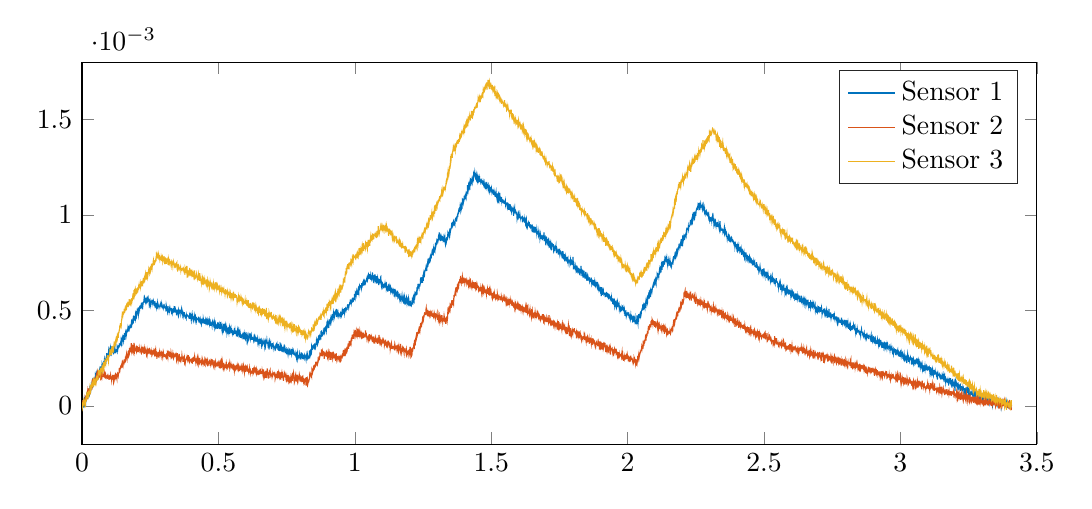
\begin{tikzpicture}

\begin{axis}[%
width=\textwidth,
height=0.4\textwidth,
at={(0\textwidth,0\textwidth)},
scale only axis,
xmin=0,
xmax=3.5,
ymin=-0.0002,
ymax=0.0018,
axis background/.style={fill=white},
title style={font=\bfseries},
% title={Created strains, 20 m/s},
legend style={legend cell align=left,align=left,draw=white!15!black}
]
\addplot [color=mycolor1,solid]
  table[row sep=crcr]{%
0	5.61763492542188e-06\\
0.0009765625	8.2480239238617e-06\\
0.001953125	2.94852619220291e-05\\
0.0029296875	1.28259755671245e-05\\
0.00390625	1.75544294558401e-05\\
0.0048828125	7.61982308695439e-06\\
0.005859375	1.63186304634494e-05\\
0.0068359375	8.87600165440393e-06\\
0.0078125	2.74660028947526e-05\\
0.0087890625	1.80643169848134e-05\\
0.009765625	4.11571848595412e-05\\
0.0107421875	4.00486565591226e-05\\
0.01171875	3.23483858722773e-05\\
0.0126953125	3.2183209952279e-05\\
0.013671875	2.47685785107283e-05\\
0.0146484375	4.97704887393195e-05\\
0.015625	5.25963091692072e-05\\
0.0166015625	4.57701563352997e-05\\
0.017578125	7.05569374619179e-05\\
0.0185546875	5.82093843187586e-05\\
0.01953125	6.1038310719137e-05\\
0.0205078125	5.8000583913858e-05\\
0.021484375	6.82067150725505e-05\\
0.0224609375	5.58430455620477e-05\\
0.0234375	6.50590888529318e-05\\
0.0244140625	5.88207577155528e-05\\
0.025390625	5.92113637487486e-05\\
0.0263671875	5.58983663180581e-05\\
0.02734375	9.2923356499796e-05\\
0.0283203125	5.94582703508318e-05\\
0.029296875	0.000106079963590784\\
0.0302734375	9.29190443360419e-05\\
0.03125	6.68829969614059e-05\\
0.0322265625	8.9876911112748e-05\\
0.033203125	0.00010237955806443\\
0.0341796875	8.93985388000974e-05\\
0.03515625	0.000106990409241695\\
0.0361328125	9.14066642879265e-05\\
0.037109375	0.000105517051374405\\
0.0380859375	0.000122523247706333\\
0.0390625	0.00011377923132816\\
0.0400390625	0.000125177898352353\\
0.041015625	0.000116194051085279\\
0.0419921875	0.000111486594810914\\
0.04296875	0.000126176160169465\\
0.0439453125	0.000124328420237567\\
0.044921875	0.000147843610250712\\
0.0458984375	0.000121097353263401\\
0.046875	0.00013303416803015\\
0.0478515625	0.000120177891489657\\
0.048828125	0.000153816110647393\\
0.0498046875	0.000146901429483939\\
0.05078125	0.000157219020637944\\
0.0517578125	0.000143266590485095\\
0.052734375	0.000153054053366891\\
0.0537109375	0.000164314398864883\\
0.0546875	0.000151118492344592\\
0.0556640625	0.000162494749745378\\
0.056640625	0.000145496645537222\\
0.0576171875	0.000159373076347379\\
0.05859375	0.000163859896106116\\
0.0595703125	0.000160806026519213\\
0.060546875	0.000154787040021132\\
0.0615234375	0.000176183961433721\\
0.0625	0.000178461067782924\\
0.0634765625	0.000185034418650242\\
0.064453125	0.000191246082411131\\
0.0654296875	0.000175566514581635\\
0.06640625	0.000189685590146137\\
0.0673828125	0.000191263823158752\\
0.068359375	0.000204540082950693\\
0.0693359375	0.000204562897573507\\
0.0703125	0.00019022796099192\\
0.0712890625	0.000182666665972532\\
0.072265625	0.000195449790185512\\
0.0732421875	0.000216208496071812\\
0.07421875	0.000208996291362654\\
0.0751953125	0.000209783851607069\\
0.076171875	0.000207604532012209\\
0.0771484375	0.000211072643279371\\
0.078125	0.000224705847142723\\
0.0791015625	0.000230406028968652\\
0.080078125	0.000230639651606244\\
0.0810546875	0.000230126751517769\\
0.08203125	0.000242767700102659\\
0.0830078125	0.000232024444749484\\
0.083984375	0.000236416489590182\\
0.0849609375	0.000229535057024595\\
0.0859375	0.000244087276129774\\
0.0869140625	0.000243357350813527\\
0.087890625	0.000237384268256193\\
0.0888671875	0.00025588643916727\\
0.08984375	0.000255784837661185\\
0.0908203125	0.000276450606331177\\
0.091796875	0.000263753999474906\\
0.0927734375	0.000266515851252011\\
0.09375	0.000262324518355651\\
0.0947265625	0.000255915299343183\\
0.095703125	0.000257727243047264\\
0.0966796875	0.000275725012024704\\
0.09765625	0.000290429841269554\\
0.0986328125	0.000281621160143543\\
0.099609375	0.000290126404707007\\
0.1005859375	0.000278443592898531\\
0.1015625	0.000289231571182172\\
0.1025390625	0.00028620882364362\\
0.103515625	0.000283675972126308\\
0.1044921875	0.000301045367794996\\
0.10546875	0.000290548551846065\\
0.1064453125	0.000260934431958766\\
0.107421875	0.000312201199965517\\
0.1083984375	0.000289615627113654\\
0.109375	0.000296182716061239\\
0.1103515625	0.000287558726572705\\
0.111328125	0.000293416891290423\\
0.1123046875	0.000288989356888844\\
0.11328125	0.000290737215482653\\
0.1142578125	0.000286752440534289\\
0.115234375	0.000279814434166461\\
0.1162109375	0.000286012966814586\\
0.1171875	0.000293292214867238\\
0.1181640625	0.000288152418717252\\
0.119140625	0.000305826606945362\\
0.1201171875	0.000320554001131996\\
0.12109375	0.000281791320380304\\
0.1220703125	0.000280375408167599\\
0.123046875	0.000278318766947845\\
0.1240234375	0.000278842375340567\\
0.125	0.000287226987849083\\
0.1259765625	0.000294302915682257\\
0.126953125	0.00029489809649885\\
0.1279296875	0.000282781507394749\\
0.12890625	0.000313607668029632\\
0.1298828125	0.000310437500719953\\
0.130859375	0.000293490070561613\\
0.1318359375	0.000303480520118192\\
0.1328125	0.000303495142604498\\
0.1337890625	0.000310242014375114\\
0.134765625	0.000306955099910096\\
0.1357421875	0.000308701659798706\\
0.13671875	0.00032016965436265\\
0.1376953125	0.000317830191365449\\
0.138671875	0.000323335014601095\\
0.1396484375	0.000322342171871774\\
0.140625	0.000326909299149157\\
0.1416015625	0.000332999330906215\\
0.142578125	0.000326817815838835\\
0.1435546875	0.000349715672352692\\
0.14453125	0.000344411756987469\\
0.1455078125	0.000313307154528726\\
0.146484375	0.000336734685829313\\
0.1474609375	0.000352301592855857\\
0.1484375	0.000357720289798072\\
0.1494140625	0.00033659885407544\\
0.150390625	0.000371027824695656\\
0.1513671875	0.00035546730712202\\
0.15234375	0.000343339188528898\\
0.1533203125	0.000356616434116109\\
0.154296875	0.000356873796022695\\
0.1552734375	0.000381571839377209\\
0.15625	0.000346457441660023\\
0.1572265625	0.000362797613886762\\
0.158203125	0.000377237648709199\\
0.1591796875	0.000383299034970395\\
0.16015625	0.000362122248197499\\
0.1611328125	0.000394551273293012\\
0.162109375	0.000369283251873805\\
0.1630859375	0.000377050604307935\\
0.1640625	0.000384907294419733\\
0.1650390625	0.000399301902251814\\
0.166015625	0.00039888143117045\\
0.1669921875	0.000395925634517849\\
0.16796875	0.000407148575778156\\
0.1689453125	0.000395440579992023\\
0.169921875	0.000419098770452326\\
0.1708984375	0.000406796690405189\\
0.171875	0.000389962270624031\\
0.1728515625	0.000401837800296045\\
0.173828125	0.000403522609576838\\
0.1748046875	0.000404581426781273\\
0.17578125	0.000424988192324995\\
0.1767578125	0.000408802797873613\\
0.177734375	0.000423379589132802\\
0.1787109375	0.000424666789856893\\
0.1796875	0.000420646613593277\\
0.1806640625	0.000431971335048709\\
0.181640625	0.000426357412382679\\
0.1826171875	0.000454364376301335\\
0.18359375	0.000423284999294679\\
0.1845703125	0.000443536964243192\\
0.185546875	0.000438389407834792\\
0.1865234375	0.00044379212211266\\
0.1875	0.000431083984379951\\
0.1884765625	0.000459304847280307\\
0.189453125	0.000455549916926866\\
0.1904296875	0.000466845595158246\\
0.19140625	0.000464601307906717\\
0.1923828125	0.000452935982770261\\
0.193359375	0.000451173125487647\\
0.1943359375	0.000460783759562636\\
0.1953125	0.000473588119874218\\
0.1962890625	0.000459843995770283\\
0.197265625	0.000470945120898989\\
0.1982421875	0.000454037291207491\\
0.19921875	0.000468551093229787\\
0.2001953125	0.00048563034149191\\
0.201171875	0.000491561126050219\\
0.2021484375	0.000499806292008056\\
0.203125	0.000492596614270554\\
0.2041015625	0.000494510857364399\\
0.205078125	0.000483616075549548\\
0.2060546875	0.000476111315086283\\
0.20703125	0.000508345365333321\\
0.2080078125	0.00050628107015831\\
0.208984375	0.000507856634396387\\
0.2099609375	0.000512444262898857\\
0.2109375	0.000504022801126241\\
0.2119140625	0.000522129802184994\\
0.212890625	0.000523002514901955\\
0.2138671875	0.000513018581329183\\
0.21484375	0.00051224572208681\\
0.2158203125	0.000520399604447598\\
0.216796875	0.000530098236833961\\
0.2177734375	0.000537405763625898\\
0.21875	0.000538302149870282\\
0.2197265625	0.000511979378904934\\
0.220703125	0.000536354842690119\\
0.2216796875	0.000505220759439539\\
0.22265625	0.000522422321836277\\
0.2236328125	0.000532447560229401\\
0.224609375	0.00054385337586083\\
0.2255859375	0.000545335128320518\\
0.2265625	0.000547186412817513\\
0.2275390625	0.000561284729703229\\
0.228515625	0.000554586249568084\\
0.2294921875	0.000563986871426548\\
0.23046875	0.000553908144006615\\
0.2314453125	0.000545024670219173\\
0.232421875	0.000541805201363195\\
0.2333984375	0.000565165284173371\\
0.234375	0.000548507515999258\\
0.2353515625	0.000557005962406137\\
0.236328125	0.000551600799396097\\
0.2373046875	0.000545927668475756\\
0.23828125	0.000555269883597719\\
0.2392578125	0.000541739997926481\\
0.240234375	0.00055886643924596\\
0.2412109375	0.000561947056241361\\
0.2421875	0.000566866015559865\\
0.2431640625	0.00055492074553384\\
0.244140625	0.000557015935936016\\
0.2451171875	0.00055504309777553\\
0.24609375	0.000536577937312149\\
0.2470703125	0.00054500597457877\\
0.248046875	0.000549850108355468\\
0.2490234375	0.000533728347558309\\
0.25	0.000542422692658743\\
0.2509765625	0.000529992749698708\\
0.251953125	0.000541033262118532\\
0.2529296875	0.000545435938192689\\
0.25390625	0.000546016243316443\\
0.2548828125	0.000548988951607388\\
0.255859375	0.000551461086062596\\
0.2568359375	0.000538997919737561\\
0.2578125	0.000550264842544894\\
0.2587890625	0.000550501620712441\\
0.259765625	0.000538082322609025\\
0.2607421875	0.000540258567701582\\
0.26171875	0.000547744439818302\\
0.2626953125	0.000537488964579556\\
0.263671875	0.000530381429862801\\
0.2646484375	0.000532064586789957\\
0.265625	0.000530213228285613\\
0.2666015625	0.000525306233200883\\
0.267578125	0.00054797560234567\\
0.2685546875	0.00051429585166304\\
0.26953125	0.00053372380094928\\
0.2705078125	0.000535441029693905\\
0.271484375	0.000535707096631609\\
0.2724609375	0.000531008758054062\\
0.2734375	0.000517373123452871\\
0.2744140625	0.000526700166871204\\
0.275390625	0.000521363630337096\\
0.2763671875	0.000538016711618773\\
0.27734375	0.000526707751784212\\
0.2783203125	0.000534896523359094\\
0.279296875	0.000529004803591426\\
0.2802734375	0.000523548256355133\\
0.28125	0.000521284156633257\\
0.2822265625	0.000514271323874376\\
0.283203125	0.000519645181887694\\
0.2841796875	0.000521024120156414\\
0.28515625	0.000525533475060375\\
0.2861328125	0.000530277692637596\\
0.287109375	0.000527935454063944\\
0.2880859375	0.000533704207014916\\
0.2890625	0.00052511538008739\\
0.2900390625	0.000534366172987027\\
0.291015625	0.000521812155454589\\
0.2919921875	0.000520230196060647\\
0.29296875	0.00053078291473059\\
0.2939453125	0.000525353594645974\\
0.294921875	0.000523013413797196\\
0.2958984375	0.000516618937801464\\
0.296875	0.000519098052476861\\
0.2978515625	0.000511337832905131\\
0.298828125	0.000517700180498606\\
0.2998046875	0.000521075501303001\\
0.30078125	0.000534574822169804\\
0.3017578125	0.000513706004146764\\
0.302734375	0.000513405124452123\\
0.3037109375	0.00051938231993824\\
0.3046875	0.000518087679097592\\
0.3056640625	0.000516219921574352\\
0.306640625	0.000516698402752294\\
0.3076171875	0.00049462649642608\\
0.30859375	0.000527761505974932\\
0.3095703125	0.000520301005284404\\
0.310546875	0.000509427349418004\\
0.3115234375	0.000506573204757016\\
0.3125	0.000505717322648161\\
0.3134765625	0.000495325498942388\\
0.314453125	0.000509135891856032\\
0.3154296875	0.000523050526191076\\
0.31640625	0.000494980643146956\\
0.3173828125	0.00049266387645202\\
0.318359375	0.000509374216856041\\
0.3193359375	0.000495632665230975\\
0.3203125	0.000505741899265041\\
0.3212890625	0.000500600700916265\\
0.322265625	0.000511929998475565\\
0.3232421875	0.000502799752769303\\
0.32421875	0.000507830087265816\\
0.3251953125	0.000510316604271667\\
0.326171875	0.000509658834605147\\
0.3271484375	0.000509947025301689\\
0.328125	0.000501675861193765\\
0.3291015625	0.000479413739773222\\
0.330078125	0.000506130004143626\\
0.3310546875	0.000493815582265944\\
0.33203125	0.000507925159275399\\
0.3330078125	0.000488842981834743\\
0.333984375	0.000511845743852858\\
0.3349609375	0.000492092245600012\\
0.3359375	0.000494046124055495\\
0.3369140625	0.00050408539688222\\
0.337890625	0.000523056194023464\\
0.3388671875	0.000489649527562211\\
0.33984375	0.000516496897147584\\
0.3408203125	0.000503005627708536\\
0.341796875	0.000488671296798382\\
0.3427734375	0.000504742117398355\\
0.34375	0.000498817621742221\\
0.3447265625	0.000491399465202502\\
0.345703125	0.00049122718769572\\
0.3466796875	0.000474583669235713\\
0.34765625	0.000492989109228404\\
0.3486328125	0.000499403932392706\\
0.349609375	0.000496241066984641\\
0.3505859375	0.000489775860618973\\
0.3515625	0.000503245359502701\\
0.3525390625	0.000488129994185187\\
0.353515625	0.000497751876286066\\
0.3544921875	0.000479515139170365\\
0.35546875	0.000488661813884269\\
0.3564453125	0.000492954561678597\\
0.357421875	0.000496803183355693\\
0.3583984375	0.000489477293316759\\
0.359375	0.000492021231869238\\
0.3603515625	0.000500650159899827\\
0.361328125	0.000500030436129954\\
0.3623046875	0.000481456741338075\\
0.36328125	0.000488933542476705\\
0.3642578125	0.000501560173567735\\
0.365234375	0.000487255973037307\\
0.3662109375	0.000485400559691351\\
0.3671875	0.000498773352277469\\
0.3681640625	0.000493004707433117\\
0.369140625	0.000477013090908906\\
0.3701171875	0.000483121116949864\\
0.37109375	0.000471341804470732\\
0.3720703125	0.000479594968779008\\
0.373046875	0.000490568025300974\\
0.3740234375	0.000468199776057962\\
0.375	0.000490796251849457\\
0.3759765625	0.000476237014444067\\
0.376953125	0.000472604644478519\\
0.3779296875	0.000471734113396888\\
0.37890625	0.000457280307305122\\
0.3798828125	0.000477134576904525\\
0.380859375	0.000466056032894951\\
0.3818359375	0.00046028419740387\\
0.3828125	0.00047652538679702\\
0.3837890625	0.000470199705262176\\
0.384765625	0.000471581383252321\\
0.3857421875	0.000476315560666781\\
0.38671875	0.000476216646280282\\
0.3876953125	0.000470571400713785\\
0.388671875	0.000470718793754446\\
0.3896484375	0.000469092786731985\\
0.390625	0.000470006649421746\\
0.3916015625	0.000462715101836847\\
0.392578125	0.000458494545890219\\
0.3935546875	0.000459815746166688\\
0.39453125	0.000475846656879034\\
0.3955078125	0.000470121848531036\\
0.396484375	0.000478565457389637\\
0.3974609375	0.000480866078131339\\
0.3984375	0.000460928568380924\\
0.3994140625	0.000457498266408905\\
0.400390625	0.000448958027355682\\
0.4013671875	0.000464952697070764\\
0.40234375	0.000473476176447068\\
0.4033203125	0.000481044637684506\\
0.404296875	0.000466322715881952\\
0.4052734375	0.000460413473241612\\
0.40625	0.00046676371324383\\
0.4072265625	0.000455842288411313\\
0.408203125	0.000464465526002111\\
0.4091796875	0.000462250480818378\\
0.41015625	0.000450173755942373\\
0.4111328125	0.000458693482445889\\
0.412109375	0.000466182570516619\\
0.4130859375	0.000475303217482231\\
0.4140625	0.000466058767010202\\
0.4150390625	0.000479480520422956\\
0.416015625	0.000452618521490565\\
0.4169921875	0.000460905014251087\\
0.41796875	0.000456884818967254\\
0.4189453125	0.000459528081824606\\
0.419921875	0.000446789263983258\\
0.4208984375	0.000456017614514211\\
0.421875	0.000453397521578732\\
0.4228515625	0.000452317884806979\\
0.423828125	0.000451907381818866\\
0.4248046875	0.000452466563704414\\
0.42578125	0.000454637105084867\\
0.4267578125	0.000467006957513192\\
0.427734375	0.000449756742373889\\
0.4287109375	0.000452993524878385\\
0.4296875	0.000436076861329295\\
0.4306640625	0.000453906387828696\\
0.431640625	0.000452352582089015\\
0.4326171875	0.000444574423005173\\
0.43359375	0.000454245826768848\\
0.4345703125	0.000447176567034124\\
0.435546875	0.000446827996600679\\
0.4365234375	0.000437749393650483\\
0.4375	0.000457314417592758\\
0.4384765625	0.000438818018496243\\
0.439453125	0.000448618232342699\\
0.4404296875	0.000448228887126334\\
0.44140625	0.000453723414739516\\
0.4423828125	0.000453429222167162\\
0.443359375	0.00043198522665578\\
0.4443359375	0.000457942425215405\\
0.4453125	0.000450270803084067\\
0.4462890625	0.000434540455517315\\
0.447265625	0.000433638507385915\\
0.4482421875	0.000438939919148355\\
0.44921875	0.000437175833201581\\
0.4501953125	0.000451688598794677\\
0.451171875	0.000451719412913509\\
0.4521484375	0.000443145342299541\\
0.453125	0.000450795385119237\\
0.4541015625	0.000441129411790945\\
0.455078125	0.000452796679490684\\
0.4560546875	0.000451216190050077\\
0.45703125	0.00042584181855207\\
0.4580078125	0.000446391656847915\\
0.458984375	0.000441207816558585\\
0.4599609375	0.00043482991773681\\
0.4609375	0.000444935815695002\\
0.4619140625	0.000431525468551841\\
0.462890625	0.000429867267738279\\
0.4638671875	0.000440689785099028\\
0.46484375	0.000433465079742451\\
0.4658203125	0.000434979774346425\\
0.466796875	0.000444995997552333\\
0.4677734375	0.000428067239607013\\
0.46875	0.00043493919508689\\
0.4697265625	0.000439698315161529\\
0.470703125	0.000419868221319543\\
0.4716796875	0.000432049196871149\\
0.47265625	0.000428823400280772\\
0.4736328125	0.000434591819590663\\
0.474609375	0.000432139055390393\\
0.4755859375	0.000429309141075011\\
0.4765625	0.00042030339722781\\
0.4775390625	0.000437250404139689\\
0.478515625	0.000442444869460044\\
0.4794921875	0.000431938868025119\\
0.48046875	0.000434967530477137\\
0.4814453125	0.000426496599258787\\
0.482421875	0.000421569372081524\\
0.4833984375	0.000426819172019153\\
0.484375	0.000408985362657074\\
0.4853515625	0.000440604407271865\\
0.486328125	0.000432816417245158\\
0.4873046875	0.000404682824411484\\
0.48828125	0.000409382060317657\\
0.4892578125	0.000427763212324407\\
0.490234375	0.000419898930333144\\
0.4912109375	0.000420703779623819\\
0.4921875	0.000404486244834013\\
0.4931640625	0.000421261977480975\\
0.494140625	0.000421311841751848\\
0.4951171875	0.000425356879904345\\
0.49609375	0.000403778219010145\\
0.4970703125	0.000428207400120164\\
0.498046875	0.00040688791508793\\
0.4990234375	0.000417608784153207\\
0.5	0.000431636002756376\\
0.5009765625	0.000429297251315387\\
0.501953125	0.000419383651422113\\
0.5029296875	0.000425620183193941\\
0.50390625	0.000402974828560434\\
0.5048828125	0.000422240417050755\\
0.505859375	0.000422635543166878\\
0.5068359375	0.000402706910052217\\
0.5078125	0.000413888035320189\\
0.5087890625	0.000440580892255048\\
0.509765625	0.000421114602311656\\
0.5107421875	0.000423444971695635\\
0.51171875	0.000416566028677878\\
0.5126953125	0.000398416621094347\\
0.513671875	0.00039050523033601\\
0.5146484375	0.000408191792840843\\
0.515625	0.000398335378625781\\
0.5166015625	0.00039354713739969\\
0.517578125	0.000406105598647629\\
0.5185546875	0.000411311491382784\\
0.51953125	0.000429020616312349\\
0.5205078125	0.000401394271027476\\
0.521484375	0.000406394343458301\\
0.5224609375	0.000431070217926668\\
0.5234375	0.000394116571425453\\
0.5244140625	0.000406518701254282\\
0.525390625	0.000400821066735823\\
0.5263671875	0.000416161288877416\\
0.52734375	0.000403602861649568\\
0.5283203125	0.000414699609521787\\
0.529296875	0.000405602430596285\\
0.5302734375	0.000408563198479777\\
0.53125	0.000383760078648062\\
0.5322265625	0.00039264797055989\\
0.533203125	0.000386250075990019\\
0.5341796875	0.000383865971042421\\
0.53515625	0.000407595403543983\\
0.5361328125	0.000408419169709664\\
0.537109375	0.000396109414301271\\
0.5380859375	0.000387075247255458\\
0.5390625	0.000406922625951387\\
0.5400390625	0.000414224580490026\\
0.541015625	0.000402511510881747\\
0.5419921875	0.00038675526131343\\
0.54296875	0.000389983047390402\\
0.5439453125	0.000401007670747942\\
0.544921875	0.000394097248928589\\
0.5458984375	0.000403238731200458\\
0.546875	0.000382654614470847\\
0.5478515625	0.000407334815903647\\
0.548828125	0.000388593747331193\\
0.5498046875	0.000383858949632815\\
0.55078125	0.000378721788379029\\
0.5517578125	0.000398528465741007\\
0.552734375	0.000386108372217\\
0.5537109375	0.000386227646500002\\
0.5546875	0.000384695975210121\\
0.5556640625	0.000377570998720303\\
0.556640625	0.000380383738480359\\
0.5576171875	0.000385775227987387\\
0.55859375	0.000408160747117364\\
0.5595703125	0.000382199597788501\\
0.560546875	0.00039345216186595\\
0.5615234375	0.000375544418318119\\
0.5625	0.00039319522249562\\
0.5634765625	0.00039292346973905\\
0.564453125	0.00039061809924048\\
0.5654296875	0.000386678302143245\\
0.56640625	0.000364209666195832\\
0.5673828125	0.000380545106660245\\
0.568359375	0.000387474366650481\\
0.5693359375	0.000362866967211852\\
0.5703125	0.000376270132141787\\
0.5712890625	0.000391934123011395\\
0.572265625	0.000379795682400936\\
0.5732421875	0.000392520539793766\\
0.57421875	0.000375073556711492\\
0.5751953125	0.000390342980134673\\
0.576171875	0.00037905364705342\\
0.5771484375	0.000383737597980246\\
0.578125	0.000362037094299891\\
0.5791015625	0.000361158530040272\\
0.580078125	0.00038033672604534\\
0.5810546875	0.000371365516572553\\
0.58203125	0.000356200198557219\\
0.5830078125	0.00036942074168972\\
0.583984375	0.000369895295195778\\
0.5849609375	0.000364402496883854\\
0.5859375	0.00035998136453032\\
0.5869140625	0.000374166639612025\\
0.587890625	0.000374804703491516\\
0.5888671875	0.000362922874733521\\
0.58984375	0.000383684616803392\\
0.5908203125	0.000365072481805346\\
0.591796875	0.000349638986579383\\
0.5927734375	0.000369174391356635\\
0.59375	0.000376580940148957\\
0.5947265625	0.00034896889957331\\
0.595703125	0.000386218684387337\\
0.5966796875	0.000364036260917476\\
0.59765625	0.00035821352232835\\
0.5986328125	0.000368778785430881\\
0.599609375	0.000360046158618437\\
0.6005859375	0.000374437894067285\\
0.6015625	0.000377718958374875\\
0.6025390625	0.000368313166040609\\
0.603515625	0.000363383610916162\\
0.6044921875	0.000345904819924782\\
0.60546875	0.000354799572946353\\
0.6064453125	0.000362155034839282\\
0.607421875	0.000341454112088656\\
0.6083984375	0.000350396342306677\\
0.609375	0.000361930130741897\\
0.6103515625	0.00034761542547116\\
0.611328125	0.000351721565804147\\
0.6123046875	0.000361945875867299\\
0.61328125	0.000360326959396593\\
0.6142578125	0.000359117788067473\\
0.615234375	0.000381840392606589\\
0.6162109375	0.000363636818514174\\
0.6171875	0.000349634952498404\\
0.6181640625	0.000356414934702868\\
0.619140625	0.000367033883206381\\
0.6201171875	0.000373015665841605\\
0.62109375	0.000361274046817007\\
0.6220703125	0.000346146861331429\\
0.623046875	0.000360282124447958\\
0.6240234375	0.000358609350323639\\
0.625	0.000357678162021863\\
0.6259765625	0.000351388027920773\\
0.626953125	0.000349245539181571\\
0.6279296875	0.000351893096934493\\
0.62890625	0.000344434553818137\\
0.6298828125	0.000355866184273464\\
0.630859375	0.000348914927492018\\
0.6318359375	0.000362237768877815\\
0.6328125	0.000355876979424897\\
0.6337890625	0.000350183339381086\\
0.634765625	0.000360734408753022\\
0.6357421875	0.000355601860252955\\
0.63671875	0.000349818644099562\\
0.6376953125	0.000336811582581206\\
0.638671875	0.000358742849694415\\
0.6396484375	0.000343653062806389\\
0.640625	0.000340899758012904\\
0.6416015625	0.000344216574233275\\
0.642578125	0.000354097760814035\\
0.6435546875	0.000344099684396059\\
0.64453125	0.000331047437010313\\
0.6455078125	0.000339104240068845\\
0.646484375	0.000333350024830451\\
0.6474609375	0.000338193508026212\\
0.6484375	0.000327897674799272\\
0.6494140625	0.000343468028725512\\
0.650390625	0.000335961782959415\\
0.6513671875	0.000330070530403527\\
0.65234375	0.000332595961984372\\
0.6533203125	0.000350612301631561\\
0.654296875	0.000325456535948313\\
0.6552734375	0.000341767147131836\\
0.65625	0.000338095568803868\\
0.6572265625	0.000323969254586672\\
0.658203125	0.00033580558217777\\
0.6591796875	0.00032565082987613\\
0.66015625	0.000342762456301417\\
0.6611328125	0.000339415837373391\\
0.662109375	0.000332232249101025\\
0.6630859375	0.000323009792068622\\
0.6640625	0.000327202505715636\\
0.6650390625	0.000326919311580997\\
0.666015625	0.000334854024073279\\
0.6669921875	0.000343361798353781\\
0.66796875	0.000337985665746078\\
0.6689453125	0.000325447139299341\\
0.669921875	0.000310567761099892\\
0.6708984375	0.000321538124432356\\
0.671875	0.000331923088614888\\
0.6728515625	0.000317284569299385\\
0.673828125	0.000327343566575997\\
0.6748046875	0.000341620797007572\\
0.67578125	0.000342648657249665\\
0.6767578125	0.000327651566185582\\
0.677734375	0.000343090837700193\\
0.6787109375	0.000330590444676267\\
0.6796875	0.00033148094853435\\
0.6806640625	0.000329456572609195\\
0.681640625	0.0003184599444268\\
0.6826171875	0.000324849942897292\\
0.68359375	0.00032756657552446\\
0.6845703125	0.000333743834560622\\
0.685546875	0.000295674445047085\\
0.6865234375	0.000312347441910965\\
0.6875	0.000334253343025077\\
0.6884765625	0.000326405401570263\\
0.689453125	0.000321563594836716\\
0.6904296875	0.00032411078941353\\
0.69140625	0.000330217123718689\\
0.6923828125	0.000308430859191348\\
0.693359375	0.000321493451011376\\
0.6943359375	0.000298073058038305\\
0.6953125	0.000317702760889506\\
0.6962890625	0.000316842967046661\\
0.697265625	0.000327980541996093\\
0.6982421875	0.000307532721253313\\
0.69921875	0.000319833777268871\\
0.7001953125	0.000323436959988239\\
0.701171875	0.000306311219318755\\
0.7021484375	0.000315993956766362\\
0.703125	0.000312864695896942\\
0.7041015625	0.000310138234758245\\
0.705078125	0.000306393313348714\\
0.7060546875	0.000304252234359144\\
0.70703125	0.000298694998820255\\
0.7080078125	0.000305240930423653\\
0.708984375	0.000300073065752384\\
0.7099609375	0.000308411287263291\\
0.7109375	0.000324022593527858\\
0.7119140625	0.00030490893941295\\
0.712890625	0.00031708742158693\\
0.7138671875	0.000311750140851422\\
0.71484375	0.000319874782408771\\
0.7158203125	0.000305804443463983\\
0.716796875	0.000304374415962222\\
0.7177734375	0.000303355138554218\\
0.71875	0.000292192709309299\\
0.7197265625	0.000324191769419198\\
0.720703125	0.000289096318193854\\
0.7216796875	0.000301625709780181\\
0.72265625	0.000298700269906237\\
0.7236328125	0.000302600804293709\\
0.724609375	0.000287052139026601\\
0.7255859375	0.000308648721481479\\
0.7265625	0.000299930676751496\\
0.7275390625	0.000297572294108769\\
0.728515625	0.00031357891491368\\
0.7294921875	0.000305607578022384\\
0.73046875	0.000315548070616282\\
0.7314453125	0.000311004283695032\\
0.732421875	0.000291887302413479\\
0.7333984375	0.000294299821341172\\
0.734375	0.000308829694858845\\
0.7353515625	0.000291685810966006\\
0.736328125	0.000294604777670426\\
0.7373046875	0.000290366245391481\\
0.73828125	0.000298528663569089\\
0.7392578125	0.000304607344665813\\
0.740234375	0.000287264861180864\\
0.7412109375	0.000287834904080935\\
0.7421875	0.000301890218868315\\
0.7431640625	0.000308954318277895\\
0.744140625	0.00030087578055402\\
0.7451171875	0.000277122472657147\\
0.74609375	0.000289666400156787\\
0.7470703125	0.000292995024958627\\
0.748046875	0.000290077641805656\\
0.7490234375	0.000283559239355674\\
0.75	0.000270789976494633\\
0.7509765625	0.000299916876038818\\
0.751953125	0.000297962596681904\\
0.7529296875	0.000294079095826536\\
0.75390625	0.000282567740791746\\
0.7548828125	0.000272699992351067\\
0.755859375	0.000291179833823647\\
0.7568359375	0.000276231135850422\\
0.7578125	0.000281945806793616\\
0.7587890625	0.000296339533434821\\
0.759765625	0.000292957425006494\\
0.7607421875	0.000279550247876444\\
0.76171875	0.00028600312907402\\
0.7626953125	0.000275212084321747\\
0.763671875	0.000273497582285916\\
0.7646484375	0.000278857996493544\\
0.765625	0.000267468802325613\\
0.7666015625	0.000298721213542679\\
0.767578125	0.000284375800585545\\
0.7685546875	0.000271212949000853\\
0.76953125	0.000278266059974626\\
0.7705078125	0.000287440111634224\\
0.771484375	0.000275597079304527\\
0.7724609375	0.000274535621174834\\
0.7734375	0.000284111479622586\\
0.7744140625	0.000290598297945534\\
0.775390625	0.000284019930145615\\
0.7763671875	0.000276189675353242\\
0.77734375	0.00027963645082723\\
0.7783203125	0.000274062743705683\\
0.779296875	0.000268847109959678\\
0.7802734375	0.000266244723478262\\
0.78125	0.000264476872606548\\
0.7822265625	0.000263357839698534\\
0.783203125	0.00027143627117431\\
0.7841796875	0.000254942872905178\\
0.78515625	0.000269045965180119\\
0.7861328125	0.000254693474901238\\
0.787109375	0.00026664123924812\\
0.7880859375	0.000259621846299284\\
0.7890625	0.000269782180612787\\
0.7900390625	0.000277554777027792\\
0.791015625	0.000250523118469008\\
0.7919921875	0.000259335645950266\\
0.79296875	0.000258831445867913\\
0.7939453125	0.000261213856853307\\
0.794921875	0.000263382038264784\\
0.7958984375	0.00025552935498831\\
0.796875	0.000261756270198463\\
0.7978515625	0.000273751075467081\\
0.798828125	0.000264758247819137\\
0.7998046875	0.000257826650234092\\
0.80078125	0.000265370938670044\\
0.8017578125	0.000267255051108967\\
0.802734375	0.0002435491339164\\
0.8037109375	0.000259066350829212\\
0.8046875	0.000280181349042897\\
0.8056640625	0.000260387198232592\\
0.806640625	0.000261060868208304\\
0.8076171875	0.000274575325968264\\
0.80859375	0.000246262547380234\\
0.8095703125	0.00026634179852631\\
0.810546875	0.000254237417476276\\
0.8115234375	0.000259290138791301\\
0.8125	0.000262335985939596\\
0.8134765625	0.000253731647920401\\
0.814453125	0.000248948121918637\\
0.8154296875	0.000261227752767708\\
0.81640625	0.00025307636508184\\
0.8173828125	0.00025489331678978\\
0.818359375	0.000259270370123565\\
0.8193359375	0.000261818146622731\\
0.8203125	0.000249822294424792\\
0.8212890625	0.000242071397285033\\
0.822265625	0.000255564669271098\\
0.8232421875	0.000263908561245268\\
0.82421875	0.000244102245025038\\
0.8251953125	0.000255346110056692\\
0.826171875	0.00026674507946102\\
0.8271484375	0.000254124172912936\\
0.828125	0.000260408322532834\\
0.8291015625	0.000258250181352839\\
0.830078125	0.000252355804689688\\
0.8310546875	0.000255844829725247\\
0.83203125	0.000253796552910384\\
0.8330078125	0.000266673096527848\\
0.833984375	0.000288633289750327\\
0.8349609375	0.000275192024385702\\
0.8359375	0.000291385899746153\\
0.8369140625	0.000268375430937751\\
0.837890625	0.000274611036735131\\
0.8388671875	0.000299199210015229\\
0.83984375	0.000270516917973149\\
0.8408203125	0.000273319100307713\\
0.841796875	0.000308573309843528\\
0.8427734375	0.000300703081757981\\
0.84375	0.00029545985944405\\
0.8447265625	0.000295994674159749\\
0.845703125	0.000308764140933182\\
0.8466796875	0.000306359412002458\\
0.84765625	0.000309629687844336\\
0.8486328125	0.000318721219508177\\
0.849609375	0.00031946817070236\\
0.8505859375	0.000311256041426396\\
0.8515625	0.000297616904059621\\
0.8525390625	0.000327063811227649\\
0.853515625	0.000305595669182775\\
0.8544921875	0.000292928802361752\\
0.85546875	0.000323913756944168\\
0.8564453125	0.000323851771962158\\
0.857421875	0.000318727755910414\\
0.8583984375	0.000328354297270394\\
0.859375	0.00034296538214376\\
0.8603515625	0.000334811945170887\\
0.861328125	0.000330738366774578\\
0.8623046875	0.000336910784801335\\
0.86328125	0.000321524293828396\\
0.8642578125	0.000325475145677824\\
0.865234375	0.000331923039255989\\
0.8662109375	0.000333422206523986\\
0.8671875	0.000369190224272641\\
0.8681640625	0.000355075074265734\\
0.869140625	0.000361498239750019\\
0.8701171875	0.000350973374930824\\
0.87109375	0.000348798265589933\\
0.8720703125	0.000366337667099407\\
0.873046875	0.000364711750549536\\
0.8740234375	0.000358625914886651\\
0.875	0.000347190680115348\\
0.8759765625	0.000388252559351143\\
0.876953125	0.00038982246152413\\
0.8779296875	0.000361165345666318\\
0.87890625	0.000386597673569057\\
0.8798828125	0.000373422255548231\\
0.880859375	0.000372426378689717\\
0.8818359375	0.000370486878973068\\
0.8828125	0.000378546562642497\\
0.8837890625	0.000387033892686625\\
0.884765625	0.000373272832408447\\
0.8857421875	0.00039101879653367\\
0.88671875	0.000376758148156582\\
0.8876953125	0.000392656079712255\\
0.888671875	0.000387050923792862\\
0.8896484375	0.00041142389328933\\
0.890625	0.000394097591053587\\
0.8916015625	0.000401120488445168\\
0.892578125	0.000409898710220468\\
0.8935546875	0.000405797157607138\\
0.89453125	0.000404351304367674\\
0.8955078125	0.000394715740022121\\
0.896484375	0.00041068418948362\\
0.8974609375	0.000428285287474392\\
0.8984375	0.000423313818628879\\
0.8994140625	0.000409782086890685\\
0.900390625	0.000433183432137593\\
0.9013671875	0.000424493973668563\\
0.90234375	0.000435524920580492\\
0.9033203125	0.000431894671983218\\
0.904296875	0.000409427817507436\\
0.9052734375	0.000424214237772627\\
0.90625	0.000453097026032585\\
0.9072265625	0.000437477266414294\\
0.908203125	0.000435511083085323\\
0.9091796875	0.000446603831875485\\
0.91015625	0.000451872846849148\\
0.9111328125	0.000441109945000605\\
0.912109375	0.000453689932042901\\
0.9130859375	0.000440205889295897\\
0.9140625	0.000448297167586636\\
0.9150390625	0.00045112513457602\\
0.916015625	0.000461517105951107\\
0.9169921875	0.000481047580732936\\
0.91796875	0.000470096699549899\\
0.9189453125	0.000457268588020507\\
0.919921875	0.000451847672286492\\
0.9208984375	0.000463045766578857\\
0.921875	0.000488072704267978\\
0.9228515625	0.000480599007359779\\
0.923828125	0.000466759906831274\\
0.9248046875	0.000493211363877482\\
0.92578125	0.00047367767443075\\
0.9267578125	0.000484019109962876\\
0.927734375	0.000479617395945312\\
0.9287109375	0.000488756321745847\\
0.9296875	0.000482935831487417\\
0.9306640625	0.000481616889236323\\
0.931640625	0.000480863722246982\\
0.9326171875	0.00050788190472085\\
0.93359375	0.000466728588011603\\
0.9345703125	0.000496267773824162\\
0.935546875	0.000480653137219743\\
0.9365234375	0.000490046411308774\\
0.9375	0.000494128120071196\\
0.9384765625	0.000468365085061243\\
0.939453125	0.000489687873171029\\
0.9404296875	0.000478984013473432\\
0.94140625	0.000470474368316037\\
0.9423828125	0.000479710402493376\\
0.943359375	0.000478357987199939\\
0.9443359375	0.000481607366895789\\
0.9453125	0.000481813210455807\\
0.9462890625	0.000473971651969327\\
0.947265625	0.000483758712097133\\
0.9482421875	0.000478601854915656\\
0.94921875	0.000487514328726484\\
0.9501953125	0.000488810731962328\\
0.951171875	0.000471666767202302\\
0.9521484375	0.000475806433861559\\
0.953125	0.000491273686204543\\
0.9541015625	0.000502844949100265\\
0.955078125	0.000497546658356184\\
0.9560546875	0.000486563243683295\\
0.95703125	0.000490689068003759\\
0.9580078125	0.000506667053203497\\
0.958984375	0.000481346840486474\\
0.9599609375	0.00049211313228344\\
0.9609375	0.000488654056894617\\
0.9619140625	0.000512543243278789\\
0.962890625	0.000488068328306462\\
0.9638671875	0.000497360581162902\\
0.96484375	0.0005051771857239\\
0.9658203125	0.000509874506037514\\
0.966796875	0.000504602847275324\\
0.9677734375	0.000500409884948623\\
0.96875	0.00050926067675159\\
0.9697265625	0.000511314998156606\\
0.970703125	0.000504721267388098\\
0.9716796875	0.000505190545581781\\
0.97265625	0.000522611831501952\\
0.9736328125	0.000529518530065786\\
0.974609375	0.000529910149201615\\
0.9755859375	0.000526571437915363\\
0.9765625	0.000522308221159858\\
0.9775390625	0.000513984784539687\\
0.978515625	0.000522480565036874\\
0.9794921875	0.000528360382843708\\
0.98046875	0.000533597567941208\\
0.9814453125	0.000541004028374259\\
0.982421875	0.000542780248961637\\
0.9833984375	0.000550757690917757\\
0.984375	0.000547977477869015\\
0.9853515625	0.000532562398063722\\
0.986328125	0.000556341060487804\\
0.9873046875	0.000539733460752674\\
0.98828125	0.000547745374520694\\
0.9892578125	0.000547079988268014\\
0.990234375	0.000562753854544317\\
0.9912109375	0.000540783971909581\\
0.9921875	0.000566324838390957\\
0.9931640625	0.000554925770777988\\
0.994140625	0.000555678744349839\\
0.9951171875	0.00055289811711456\\
0.99609375	0.000559876985163684\\
0.9970703125	0.000557850667929526\\
0.998046875	0.000563085523940424\\
0.9990234375	0.000585890068031439\\
1	0.000574217998267458\\
1.0009765625	0.000567498818043694\\
1.001953125	0.000591927059125475\\
1.0029296875	0.000588181668277577\\
1.00390625	0.00058792665715214\\
1.0048828125	0.000580654401262624\\
1.005859375	0.000594837851340233\\
1.0068359375	0.000583643919365804\\
1.0078125	0.000584254503332547\\
1.0087890625	0.000588052564716843\\
1.009765625	0.000591572396123591\\
1.0107421875	0.000603398768477551\\
1.01171875	0.00060917601863726\\
1.0126953125	0.000582156875302547\\
1.013671875	0.000599540382584556\\
1.0146484375	0.000591713734029786\\
1.015625	0.000620212543624332\\
1.0166015625	0.000626240150928806\\
1.017578125	0.000605681343714351\\
1.0185546875	0.000622886926630534\\
1.01953125	0.000621745666137942\\
1.0205078125	0.000622121666240871\\
1.021484375	0.000629464105389046\\
1.0224609375	0.000629776020147272\\
1.0234375	0.000626633704886666\\
1.0244140625	0.000618972395711887\\
1.025390625	0.000643458218892438\\
1.0263671875	0.000620322056413973\\
1.02734375	0.000631512016054666\\
1.0283203125	0.000630940733220165\\
1.029296875	0.000646474938586203\\
1.0302734375	0.000650355254656455\\
1.03125	0.000653450306657962\\
1.0322265625	0.00065659983121774\\
1.033203125	0.000630346056269922\\
1.0341796875	0.00065017906151327\\
1.03515625	0.000648661693579087\\
1.0361328125	0.000644260844679733\\
1.037109375	0.000654393197725862\\
1.0380859375	0.00065141719381558\\
1.0390625	0.000644175712656773\\
1.0400390625	0.000650508857217978\\
1.041015625	0.000650908023656232\\
1.0419921875	0.000653567939325914\\
1.04296875	0.000663231130608475\\
1.0439453125	0.00066854260618975\\
1.044921875	0.000658732187897485\\
1.0458984375	0.000655034366396604\\
1.046875	0.00066200553674409\\
1.0478515625	0.00068062715045167\\
1.048828125	0.000685189249960053\\
1.0498046875	0.000664318761598991\\
1.05078125	0.000684053026442149\\
1.0517578125	0.000678012478424702\\
1.052734375	0.000675214899193899\\
1.0537109375	0.000689369834238764\\
1.0546875	0.000673289060749157\\
1.0556640625	0.000672409983289108\\
1.056640625	0.00068135819247074\\
1.0576171875	0.000660976710710583\\
1.05859375	0.000675055446750071\\
1.0595703125	0.000668753826990729\\
1.060546875	0.000663323331352619\\
1.0615234375	0.000671289728605299\\
1.0625	0.000679557755835605\\
1.0634765625	0.000674991961587914\\
1.064453125	0.000699122518664271\\
1.0654296875	0.000674418632684654\\
1.06640625	0.000666244522412494\\
1.0673828125	0.000681218040520577\\
1.068359375	0.000679320885531007\\
1.0693359375	0.000662689458366058\\
1.0703125	0.000669953898052953\\
1.0712890625	0.000658370728421432\\
1.072265625	0.00066539884165407\\
1.0732421875	0.000664905098098768\\
1.07421875	0.000688165943577009\\
1.0751953125	0.000672909377370695\\
1.076171875	0.000653302632714268\\
1.0771484375	0.000649667647971317\\
1.078125	0.000655971353690004\\
1.0791015625	0.000665559811982671\\
1.080078125	0.000679856268451191\\
1.0810546875	0.000653976906456658\\
1.08203125	0.000657392032001791\\
1.0830078125	0.000642247378413148\\
1.083984375	0.00066920270881598\\
1.0849609375	0.000662046150283665\\
1.0859375	0.00066394141770895\\
1.0869140625	0.000661479113874736\\
1.087890625	0.000632278099811669\\
1.0888671875	0.000663372419286418\\
1.08984375	0.000650488217367719\\
1.0908203125	0.000643995927956982\\
1.091796875	0.000644545045356765\\
1.0927734375	0.000659030819028063\\
1.09375	0.000666186085920227\\
1.0947265625	0.000656314984121057\\
1.095703125	0.000663269611037864\\
1.0966796875	0.000638719951724444\\
1.09765625	0.000627883319591055\\
1.0986328125	0.000638225366756552\\
1.099609375	0.000630338412851415\\
1.1005859375	0.000629054009745096\\
1.1015625	0.000635372438722518\\
1.1025390625	0.00062314538688279\\
1.103515625	0.000628076879637012\\
1.1044921875	0.000635029215492007\\
1.10546875	0.000636257415471985\\
1.1064453125	0.000626213773067412\\
1.107421875	0.000630475649318944\\
1.1083984375	0.000631835063185984\\
1.109375	0.00062754437291869\\
1.1103515625	0.000637152380456455\\
1.111328125	0.000620066711037217\\
1.1123046875	0.000632687824633418\\
1.11328125	0.000642170616896236\\
1.1142578125	0.000642846457371358\\
1.115234375	0.00061990543856128\\
1.1162109375	0.000629155053112443\\
1.1171875	0.000613352116531247\\
1.1181640625	0.000626835426652781\\
1.119140625	0.000604428623678669\\
1.1201171875	0.000602895692311396\\
1.12109375	0.000609939874545112\\
1.1220703125	0.000599796360702955\\
1.123046875	0.000622147029562131\\
1.1240234375	0.000616850295027931\\
1.125	0.00062502376586221\\
1.1259765625	0.000617212927403473\\
1.126953125	0.000619642899961255\\
1.1279296875	0.000602269391455574\\
1.12890625	0.000619811629383833\\
1.1298828125	0.000609859795855101\\
1.130859375	0.00060255522572459\\
1.1318359375	0.00061951625719612\\
1.1328125	0.000614591188167345\\
1.1337890625	0.000604255877881616\\
1.134765625	0.000607896523593707\\
1.1357421875	0.000600368416455429\\
1.13671875	0.000594658772249525\\
1.1376953125	0.000604221212035513\\
1.138671875	0.00059841181453882\\
1.1396484375	0.000596225086948612\\
1.140625	0.000602744959836165\\
1.1416015625	0.000593351812413005\\
1.142578125	0.000593850858899817\\
1.1435546875	0.000612786670700668\\
1.14453125	0.000572399134934803\\
1.1455078125	0.000586456889138207\\
1.146484375	0.000580415895790161\\
1.1474609375	0.00061248335207053\\
1.1484375	0.000588547726773884\\
1.1494140625	0.000606488880113145\\
1.150390625	0.00059089639240341\\
1.1513671875	0.000588727181463951\\
1.15234375	0.000575334109999471\\
1.1533203125	0.000575374049325195\\
1.154296875	0.00058439778357168\\
1.1552734375	0.000577872736018474\\
1.15625	0.000603778753517902\\
1.1572265625	0.000570676860749454\\
1.158203125	0.00059501483928126\\
1.1591796875	0.000584348686296897\\
1.16015625	0.00057569122118923\\
1.1611328125	0.000567753858737271\\
1.162109375	0.000569617979734017\\
1.1630859375	0.00056931102864942\\
1.1640625	0.000561593528702379\\
1.1650390625	0.000589340150712424\\
1.166015625	0.000564946884101057\\
1.1669921875	0.000559918292862613\\
1.16796875	0.000571258711227564\\
1.1689453125	0.000570288866120826\\
1.169921875	0.00055525339014634\\
1.1708984375	0.00056334063271608\\
1.171875	0.000569517391644424\\
1.1728515625	0.000578950437350709\\
1.173828125	0.000561571536598594\\
1.1748046875	0.000573300517867297\\
1.17578125	0.000546891849490964\\
1.1767578125	0.000558015875781016\\
1.177734375	0.000562797234876433\\
1.1787109375	0.000535892563254717\\
1.1796875	0.000561320562606969\\
1.1806640625	0.000551837388931834\\
1.181640625	0.000545955868940122\\
1.1826171875	0.000567824005049715\\
1.18359375	0.000558013826427909\\
1.1845703125	0.000546536196248738\\
1.185546875	0.000549385209744413\\
1.1865234375	0.000537652875692794\\
1.1875	0.000540535181303257\\
1.1884765625	0.0005637200514423\\
1.189453125	0.0005691208831934\\
1.1904296875	0.000555652212378975\\
1.19140625	0.000539690366543212\\
1.1923828125	0.00054949347260508\\
1.193359375	0.000539631793144746\\
1.1943359375	0.000537007882308268\\
1.1953125	0.000552938633743518\\
1.1962890625	0.000561988890766813\\
1.197265625	0.000543809196740941\\
1.1982421875	0.000549879979766071\\
1.19921875	0.000532088786545474\\
1.2001953125	0.000535369748715558\\
1.201171875	0.00053366018991306\\
1.2021484375	0.000549310669256759\\
1.203125	0.000530570185527179\\
1.2041015625	0.000534279398875138\\
1.205078125	0.000539087473780048\\
1.2060546875	0.000527742403435689\\
1.20703125	0.000525136665230309\\
1.2080078125	0.000535430360131192\\
1.208984375	0.00053368145133009\\
1.2099609375	0.000538639134467088\\
1.2109375	0.00055603821515736\\
1.2119140625	0.000549399058905178\\
1.212890625	0.00056194554973073\\
1.2138671875	0.00054333108754767\\
1.21484375	0.000559197466096549\\
1.2158203125	0.000550959299113368\\
1.216796875	0.000566478086678194\\
1.2177734375	0.000558088933162326\\
1.21875	0.000576265535069565\\
1.2197265625	0.000584570751262926\\
1.220703125	0.000575215301808308\\
1.2216796875	0.000584355156077434\\
1.22265625	0.000594500773381539\\
1.2236328125	0.000595696065188152\\
1.224609375	0.000592829485504707\\
1.2255859375	0.000579026235542996\\
1.2265625	0.00059431616354169\\
1.2275390625	0.000582111486184835\\
1.228515625	0.000601490940784018\\
1.2294921875	0.000617277970136623\\
1.23046875	0.000616417260923457\\
1.2314453125	0.00063916592667231\\
1.232421875	0.000616189831783278\\
1.2333984375	0.000628412899276563\\
1.234375	0.000625644610769723\\
1.2353515625	0.0006184021913083\\
1.236328125	0.00063130852832597\\
1.2373046875	0.000628513976473279\\
1.23828125	0.000628213682257653\\
1.2392578125	0.000634625354186478\\
1.240234375	0.000641867893737751\\
1.2412109375	0.000673528013201654\\
1.2421875	0.000645022984221631\\
1.2431640625	0.000646613382003608\\
1.244140625	0.000649513454566435\\
1.2451171875	0.000659956324943205\\
1.24609375	0.000674665663095886\\
1.2470703125	0.000654799000860696\\
1.248046875	0.000645081010510368\\
1.2490234375	0.000671990573964752\\
1.25	0.000686030059679773\\
1.2509765625	0.000655390464957248\\
1.251953125	0.000690712802893138\\
1.2529296875	0.000698981364587275\\
1.25390625	0.000691686804465415\\
1.2548828125	0.000673817292923489\\
1.255859375	0.000697083757422414\\
1.2568359375	0.000705996043427125\\
1.2578125	0.000712141858266354\\
1.2587890625	0.000714382166645426\\
1.259765625	0.000718094969270723\\
1.2607421875	0.000725485561264355\\
1.26171875	0.000705717295802218\\
1.2626953125	0.000731515248733538\\
1.263671875	0.000707069623414706\\
1.2646484375	0.000728643974437669\\
1.265625	0.000734848252526774\\
1.2666015625	0.00074600603688513\\
1.267578125	0.000728735298117946\\
1.2685546875	0.000743807274559392\\
1.26953125	0.000758809741050087\\
1.2705078125	0.000752864405249551\\
1.271484375	0.000759952617903362\\
1.2724609375	0.000755549088981098\\
1.2734375	0.000753382463958217\\
1.2744140625	0.000772876541988687\\
1.275390625	0.000772331670375815\\
1.2763671875	0.000780628997276891\\
1.27734375	0.00076867706333439\\
1.2783203125	0.000777231226708672\\
1.279296875	0.000790612030018105\\
1.2802734375	0.000772973825515069\\
1.28125	0.000792753558650356\\
1.2822265625	0.000795299045553471\\
1.283203125	0.000809557865441362\\
1.2841796875	0.000817183310805944\\
1.28515625	0.000814063539570501\\
1.2861328125	0.00079318626891408\\
1.287109375	0.000791545643191199\\
1.2880859375	0.00079796222982827\\
1.2890625	0.000822096397591045\\
1.2900390625	0.000813021986732671\\
1.291015625	0.000811069461398106\\
1.2919921875	0.000823376777063411\\
1.29296875	0.000827684610042256\\
1.2939453125	0.000818580488946981\\
1.294921875	0.000835916583883142\\
1.2958984375	0.000828237684348726\\
1.296875	0.000834251597882663\\
1.2978515625	0.000855104715540471\\
1.298828125	0.000844193130445412\\
1.2998046875	0.00084602952244298\\
1.30078125	0.000871484412677086\\
1.3017578125	0.000870230951379916\\
1.302734375	0.000867772362681832\\
1.3037109375	0.000870011996776677\\
1.3046875	0.000861287239547987\\
1.3056640625	0.000867019139370115\\
1.306640625	0.000885154989047687\\
1.3076171875	0.000881373972241748\\
1.30859375	0.000878830061867456\\
1.3095703125	0.000908418108144485\\
1.310546875	0.000885063348615851\\
1.3115234375	0.000883142892253824\\
1.3125	0.000883742909788727\\
1.3134765625	0.000863694139627753\\
1.314453125	0.000891651730849764\\
1.3154296875	0.000895857885639414\\
1.31640625	0.000889519479458548\\
1.3173828125	0.000870998138334737\\
1.318359375	0.000869438202593795\\
1.3193359375	0.000889465021398974\\
1.3203125	0.000873224759318347\\
1.3212890625	0.000890017456856694\\
1.322265625	0.000865998742460307\\
1.3232421875	0.000881572262336881\\
1.32421875	0.000865435693758151\\
1.3251953125	0.000868591070690555\\
1.326171875	0.000866025273397019\\
1.3271484375	0.000884189244028795\\
1.328125	0.000878537904575058\\
1.3291015625	0.000871336325381048\\
1.330078125	0.000881136755980792\\
1.3310546875	0.000857546619752478\\
1.33203125	0.000848836950030191\\
1.3330078125	0.000869217461226389\\
1.333984375	0.000865340947168124\\
1.3349609375	0.000868500740658538\\
1.3359375	0.000861649251757073\\
1.3369140625	0.000881070462048993\\
1.337890625	0.000882064491696546\\
1.3388671875	0.000866938886175798\\
1.33984375	0.000882805944207297\\
1.3408203125	0.000898421674053469\\
1.341796875	0.000888493297656951\\
1.3427734375	0.000912761603749434\\
1.34375	0.000896309009166338\\
1.3447265625	0.000896210795499483\\
1.345703125	0.000888944222682073\\
1.3466796875	0.000905054244321532\\
1.34765625	0.000913906033447618\\
1.3486328125	0.000929886138732661\\
1.349609375	0.000905999769581659\\
1.3505859375	0.000915086716806827\\
1.3515625	0.000921049364793876\\
1.3525390625	0.000926713877899391\\
1.353515625	0.000930746695236577\\
1.3544921875	0.000944330695636066\\
1.35546875	0.00093972587842831\\
1.3564453125	0.000930103904969813\\
1.357421875	0.000962820027485224\\
1.3583984375	0.000936366463560624\\
1.359375	0.000949205505130155\\
1.3603515625	0.000962967450726312\\
1.361328125	0.000966730276015701\\
1.3623046875	0.00094412700586409\\
1.36328125	0.000955583365278603\\
1.3642578125	0.000952647086538241\\
1.365234375	0.000962078654999117\\
1.3662109375	0.000965007956335683\\
1.3671875	0.000956915998895617\\
1.3681640625	0.00097651922764001\\
1.369140625	0.000980016857835672\\
1.3701171875	0.000976954248929783\\
1.37109375	0.000977527088248338\\
1.3720703125	0.000981689337549621\\
1.373046875	0.00096599211892557\\
1.3740234375	0.000979507206435039\\
1.375	0.000985220558346175\\
1.3759765625	0.000999179703743576\\
1.376953125	0.00100323062607254\\
1.3779296875	0.00100014030761451\\
1.37890625	0.00101351217992109\\
1.3798828125	0.00101353098496163\\
1.380859375	0.00102288026997342\\
1.3818359375	0.00101728324473776\\
1.3828125	0.00102195973520414\\
1.3837890625	0.00103056060041714\\
1.384765625	0.00102799333638862\\
1.3857421875	0.00104172182778353\\
1.38671875	0.00102813868024511\\
1.3876953125	0.00104228733125164\\
1.388671875	0.00103952998050085\\
1.3896484375	0.00104871228354059\\
1.390625	0.00103934260312269\\
1.3916015625	0.00105902078558986\\
1.392578125	0.00103030168535217\\
1.3935546875	0.00105078557712416\\
1.39453125	0.00108268838265127\\
1.3955078125	0.00108093604886783\\
1.396484375	0.00106840705450136\\
1.3974609375	0.00106096309631951\\
1.3984375	0.00106855845029269\\
1.3994140625	0.00107088686523541\\
1.400390625	0.00108667012230969\\
1.4013671875	0.00110084839971592\\
1.40234375	0.00108637756962853\\
1.4033203125	0.00109053915036251\\
1.404296875	0.00109281419399997\\
1.4052734375	0.00111023205996079\\
1.40625	0.00109828016230283\\
1.4072265625	0.00110756773115033\\
1.408203125	0.00109771634209925\\
1.4091796875	0.00111844449265507\\
1.41015625	0.0011019730220161\\
1.4111328125	0.00112232612966842\\
1.412109375	0.00111171882061332\\
1.4130859375	0.00115564408437945\\
1.4140625	0.00113025974597285\\
1.4150390625	0.0011229803610812\\
1.416015625	0.00113242947090553\\
1.4169921875	0.00115052597681032\\
1.41796875	0.00114126362494593\\
1.4189453125	0.00112882295874736\\
1.419921875	0.00115582970217826\\
1.4208984375	0.00114912818086445\\
1.421875	0.00114503594116557\\
1.4228515625	0.00117181839955339\\
1.423828125	0.00116309009665401\\
1.4248046875	0.00115379590832054\\
1.42578125	0.00118432282971859\\
1.4267578125	0.00118223520835653\\
1.427734375	0.00116131952703184\\
1.4287109375	0.00118008227069728\\
1.4296875	0.00118894781664342\\
1.4306640625	0.00117687874638352\\
1.431640625	0.00119187060279502\\
1.4326171875	0.00118993584406023\\
1.43359375	0.00119234813000204\\
1.4345703125	0.00118744667334711\\
1.435546875	0.00121461173398438\\
1.4365234375	0.00120929690257065\\
1.4375	0.00120741933971855\\
1.4384765625	0.00121091651804361\\
1.439453125	0.00122184873955261\\
1.4404296875	0.00120408044118992\\
1.44140625	0.00119820406702242\\
1.4423828125	0.00120786373191208\\
1.443359375	0.00121162686477461\\
1.4443359375	0.00119745992395205\\
1.4453125	0.00118719719106552\\
1.4462890625	0.00118162494225812\\
1.447265625	0.00118617354417594\\
1.4482421875	0.00121157798933328\\
1.44921875	0.00120485552224368\\
1.4501953125	0.00118198491783636\\
1.451171875	0.00119053663838976\\
1.4521484375	0.0011942585628362\\
1.453125	0.00118326896754108\\
1.4541015625	0.00119191879577027\\
1.455078125	0.00118017663829564\\
1.4560546875	0.00117495572000184\\
1.45703125	0.00117520884688124\\
1.4580078125	0.00118966123663648\\
1.458984375	0.00117795240297171\\
1.4599609375	0.0011771643235225\\
1.4609375	0.00117936250864477\\
1.4619140625	0.00116870861803088\\
1.462890625	0.00117180802769868\\
1.4638671875	0.00118248688665001\\
1.46484375	0.00118459560005876\\
1.4658203125	0.00117308834679855\\
1.466796875	0.00117442046821377\\
1.4677734375	0.0011631081708453\\
1.46875	0.00116477370398527\\
1.4697265625	0.00116425213064399\\
1.470703125	0.00117228528893835\\
1.4716796875	0.0011633024171057\\
1.47265625	0.0011759670079495\\
1.4736328125	0.00115302595568427\\
1.474609375	0.00116499617743845\\
1.4755859375	0.00115424429358221\\
1.4765625	0.00115970043304321\\
1.4775390625	0.00115937715452258\\
1.478515625	0.00113544028434234\\
1.4794921875	0.00115355065149072\\
1.48046875	0.00114743120933238\\
1.4814453125	0.00117277141287881\\
1.482421875	0.00116228800591398\\
1.4833984375	0.00114890236845751\\
1.484375	0.00114348882304102\\
1.4853515625	0.00114584655859102\\
1.486328125	0.00114915084464738\\
1.4873046875	0.00115569342707401\\
1.48828125	0.00114331008594042\\
1.4892578125	0.00115133662856583\\
1.490234375	0.00113870176394363\\
1.4912109375	0.00115195686723553\\
1.4921875	0.00113468545848424\\
1.4931640625	0.00112677564332956\\
1.494140625	0.00114800831507799\\
1.4951171875	0.00114466277427098\\
1.49609375	0.00112885698989639\\
1.4970703125	0.00112689770951949\\
1.498046875	0.00114533997318755\\
1.4990234375	0.00112721422722988\\
1.5	0.00113094317659137\\
1.5009765625	0.00113930853729845\\
1.501953125	0.00112678140993089\\
1.5029296875	0.00111563137898876\\
1.50390625	0.00112118332225714\\
1.5048828125	0.0011342235407737\\
1.505859375	0.00111433925257261\\
1.5068359375	0.00113152010891623\\
1.5078125	0.00111725855005249\\
1.5087890625	0.00110788649922227\\
1.509765625	0.0011073755724297\\
1.5107421875	0.00112412850209083\\
1.51171875	0.00111708869727359\\
1.5126953125	0.00111520420230878\\
1.513671875	0.00109640469983043\\
1.5146484375	0.00112190336014985\\
1.515625	0.00110737915294688\\
1.5166015625	0.00111158260693496\\
1.517578125	0.00111957819863432\\
1.5185546875	0.00109324622286906\\
1.51953125	0.00110790179113112\\
1.5205078125	0.00108905442117757\\
1.521484375	0.00108184972341523\\
1.5224609375	0.00111271047709627\\
1.5234375	0.00109930729080957\\
1.5244140625	0.00110158429706656\\
1.525390625	0.00108595273300102\\
1.5263671875	0.00109827572510791\\
1.52734375	0.00108558203153772\\
1.5283203125	0.00109703664283526\\
1.529296875	0.00108229286862567\\
1.5302734375	0.00109341026531139\\
1.53125	0.00111561605274161\\
1.5322265625	0.0010954455549828\\
1.533203125	0.00108116479872765\\
1.5341796875	0.00108223596145938\\
1.53515625	0.00106814608644897\\
1.5361328125	0.00108314278937008\\
1.537109375	0.00109135818148318\\
1.5380859375	0.00109108044035888\\
1.5390625	0.00107188798615278\\
1.5400390625	0.00108065067499599\\
1.541015625	0.0010787700511881\\
1.5419921875	0.00107499840934254\\
1.54296875	0.00106611417219029\\
1.5439453125	0.00106465960781835\\
1.544921875	0.00107067517813472\\
1.5458984375	0.00106517562435643\\
1.546875	0.00106381645958613\\
1.5478515625	0.00107214590274299\\
1.548828125	0.00107270117906201\\
1.5498046875	0.0010637327414261\\
1.55078125	0.00106612564493502\\
1.5517578125	0.00107423298537251\\
1.552734375	0.00105464018712593\\
1.5537109375	0.00106292015142581\\
1.5546875	0.00106295355609258\\
1.5556640625	0.00105423200624357\\
1.556640625	0.00105305539060158\\
1.5576171875	0.00105394340381153\\
1.55859375	0.0010453152730648\\
1.5595703125	0.00106632851234196\\
1.560546875	0.00105038491992751\\
1.5615234375	0.00104142086347683\\
1.5625	0.00104456760439407\\
1.5634765625	0.00106110548550112\\
1.564453125	0.00102741007297221\\
1.5654296875	0.00104920751428731\\
1.56640625	0.00105123675052754\\
1.5673828125	0.00104890603639205\\
1.568359375	0.00102645669036091\\
1.5693359375	0.00105683587298279\\
1.5703125	0.00103459765102801\\
1.5712890625	0.00103927714124206\\
1.572265625	0.00102891779150449\\
1.5732421875	0.00103335455914626\\
1.57421875	0.00101885497905685\\
1.5751953125	0.00102765102995603\\
1.576171875	0.00102199934537114\\
1.5771484375	0.00102603361568796\\
1.578125	0.00103089892434922\\
1.5791015625	0.00102683015484805\\
1.580078125	0.00103447651217386\\
1.5810546875	0.00102476543445379\\
1.58203125	0.000995154789219384\\
1.5830078125	0.00101623132683268\\
1.583984375	0.00103106476961682\\
1.5849609375	0.00102911506875535\\
1.5859375	0.00103719304253562\\
1.5869140625	0.00100866153913732\\
1.587890625	0.00102820929062604\\
1.5888671875	0.00101524881266783\\
1.58984375	0.00101934403887478\\
1.5908203125	0.0010141728938127\\
1.591796875	0.0010140577543903\\
1.5927734375	0.00101073741715084\\
1.59375	0.00100280092178685\\
1.5947265625	0.000982153348691535\\
1.595703125	0.000992271668318077\\
1.5966796875	0.000987934412070988\\
1.59765625	0.000997335843262235\\
1.5986328125	0.000976217933554696\\
1.599609375	0.00100307941699334\\
1.6005859375	0.00100803235170456\\
1.6015625	0.000982136619110501\\
1.6025390625	0.000994579856386316\\
1.603515625	0.000989414674943831\\
1.6044921875	0.000988500393738128\\
1.60546875	0.000999984948923122\\
1.6064453125	0.000988454183396978\\
1.607421875	0.000983713207696445\\
1.6083984375	0.000977158319291723\\
1.609375	0.000987950956564216\\
1.6103515625	0.000988562905669536\\
1.611328125	0.000985427266933455\\
1.6123046875	0.00098662772748334\\
1.61328125	0.000989150114017786\\
1.6142578125	0.000990838326142455\\
1.615234375	0.000973397061141167\\
1.6162109375	0.000978899592438245\\
1.6171875	0.000981321940917976\\
1.6181640625	0.000976015746513399\\
1.619140625	0.000977646252291539\\
1.6201171875	0.000962721169796717\\
1.62109375	0.00097791948968984\\
1.6220703125	0.000965567774933927\\
1.623046875	0.000967346803401546\\
1.6240234375	0.000987353716290046\\
1.625	0.000965780602809312\\
1.6259765625	0.000968379843769205\\
1.626953125	0.000939333179270543\\
1.6279296875	0.00097167408613341\\
1.62890625	0.000977569622234732\\
1.6298828125	0.000948702287226159\\
1.630859375	0.00095675603031145\\
1.6318359375	0.000950302834209029\\
1.6328125	0.00093639060418607\\
1.6337890625	0.000941602157140171\\
1.634765625	0.000953476233062185\\
1.6357421875	0.000952858835214782\\
1.63671875	0.000958290608649867\\
1.6376953125	0.00094668710954964\\
1.638671875	0.000945511310805578\\
1.6396484375	0.000963120609237484\\
1.640625	0.000939010792629501\\
1.6416015625	0.000936953171721569\\
1.642578125	0.00094882425316745\\
1.6435546875	0.000948086901166169\\
1.64453125	0.000940892806046401\\
1.6455078125	0.000940143081040132\\
1.646484375	0.000931879376855985\\
1.6474609375	0.000949666860985945\\
1.6484375	0.000938231766970633\\
1.6494140625	0.000942414178789651\\
1.650390625	0.000944835423569154\\
1.6513671875	0.000939449472637566\\
1.65234375	0.000910352968091184\\
1.6533203125	0.000940597912684355\\
1.654296875	0.00092315811817361\\
1.6552734375	0.000928255423289609\\
1.65625	0.000927710272838536\\
1.6572265625	0.000907618792989342\\
1.658203125	0.000938658759847795\\
1.6591796875	0.00092529455446464\\
1.66015625	0.000927923416205661\\
1.6611328125	0.000918268530632605\\
1.662109375	0.000923613650916009\\
1.6630859375	0.000916794105333981\\
1.6640625	0.000913146419330405\\
1.6650390625	0.000925228220572874\\
1.666015625	0.000912664810792421\\
1.6669921875	0.000901122396062881\\
1.66796875	0.000916465306239312\\
1.6689453125	0.000901794589133883\\
1.669921875	0.000902098728682969\\
1.6708984375	0.000901472661670383\\
1.671875	0.000916866735947019\\
1.6728515625	0.000905853083848529\\
1.673828125	0.000892070877088109\\
1.6748046875	0.000898648212241828\\
1.67578125	0.000906572456124351\\
1.6767578125	0.000897579700287634\\
1.677734375	0.000893234144293105\\
1.6787109375	0.00087540212532677\\
1.6796875	0.000883605662441569\\
1.6806640625	0.000894157675075324\\
1.681640625	0.000874935335897467\\
1.6826171875	0.000886969177908485\\
1.68359375	0.000885349554874029\\
1.6845703125	0.000882359551962637\\
1.685546875	0.000878532717296465\\
1.6865234375	0.000895112471218152\\
1.6875	0.000868484910439039\\
1.6884765625	0.000891398837966133\\
1.689453125	0.000879898488696689\\
1.6904296875	0.000878889802511338\\
1.69140625	0.000886646557887012\\
1.6923828125	0.000883985321700581\\
1.693359375	0.000909023270573823\\
1.6943359375	0.000862542209831059\\
1.6953125	0.000883148217525546\\
1.6962890625	0.000884946701913313\\
1.697265625	0.000879564747093271\\
1.6982421875	0.000873521130582021\\
1.69921875	0.000876418585800166\\
1.7001953125	0.000841100002757852\\
1.701171875	0.000875561776591311\\
1.7021484375	0.000870133274205423\\
1.703125	0.00087449314964629\\
1.7041015625	0.000860506715082238\\
1.705078125	0.000863213266938524\\
1.7060546875	0.000860502224540056\\
1.70703125	0.000845309688386579\\
1.7080078125	0.000875013689493512\\
1.708984375	0.000837002426929022\\
1.7099609375	0.00085666569212947\\
1.7109375	0.000847473256758209\\
1.7119140625	0.000861106124259643\\
1.712890625	0.00085316956443732\\
1.7138671875	0.000829438860831578\\
1.71484375	0.000863658093948583\\
1.7158203125	0.000841079861930962\\
1.716796875	0.000832915605746878\\
1.7177734375	0.000838355672292984\\
1.71875	0.000850855392956256\\
1.7197265625	0.000840017444027174\\
1.720703125	0.000814419557502924\\
1.7216796875	0.000855472377702376\\
1.72265625	0.000836368987806478\\
1.7236328125	0.000848381272254336\\
1.724609375	0.00084804426989294\\
1.7255859375	0.000840548228116664\\
1.7265625	0.000835629778233168\\
1.7275390625	0.000847689896925505\\
1.728515625	0.000817776669726113\\
1.7294921875	0.000824282195040979\\
1.73046875	0.000816726036952253\\
1.7314453125	0.000823607022501\\
1.732421875	0.000812203723914978\\
1.7333984375	0.0008390074421116\\
1.734375	0.000826223913157197\\
1.7353515625	0.000828612806330986\\
1.736328125	0.000827992229237203\\
1.7373046875	0.000837567928317858\\
1.73828125	0.000812856439447631\\
1.7392578125	0.000804283029191412\\
1.740234375	0.000805738258561363\\
1.7412109375	0.000821125633101972\\
1.7421875	0.000816096311706301\\
1.7431640625	0.000815894952050205\\
1.744140625	0.000814064604548214\\
1.7451171875	0.000807583696635432\\
1.74609375	0.000792087801114237\\
1.7470703125	0.000810011399873367\\
1.748046875	0.000822798280656785\\
1.7490234375	0.000793640889990402\\
1.75	0.000814325153524603\\
1.7509765625	0.00081672325056633\\
1.751953125	0.000793272188138201\\
1.7529296875	0.000800145926730484\\
1.75390625	0.000801765646941094\\
1.7548828125	0.000808869589139116\\
1.755859375	0.000807559544254949\\
1.7568359375	0.000796622822771964\\
1.7578125	0.000795429444547695\\
1.7587890625	0.00078737051201696\\
1.759765625	0.000793429910271902\\
1.7607421875	0.000772581496123067\\
1.76171875	0.000794255064675529\\
1.7626953125	0.000810764894421289\\
1.763671875	0.000797716629452392\\
1.7646484375	0.000770277434641368\\
1.765625	0.000796913395166722\\
1.7666015625	0.000766009770340912\\
1.767578125	0.000794064118783826\\
1.7685546875	0.000780670021719347\\
1.76953125	0.000763928710357575\\
1.7705078125	0.000766589876788485\\
1.771484375	0.000778308496807579\\
1.7724609375	0.000784650211004569\\
1.7734375	0.000766043100278702\\
1.7744140625	0.000761238195594146\\
1.775390625	0.000764566846795961\\
1.7763671875	0.000777348983141375\\
1.77734375	0.000777639926702779\\
1.7783203125	0.000768209581942701\\
1.779296875	0.000780667030182267\\
1.7802734375	0.000763693647211412\\
1.78125	0.000769880665423042\\
1.7822265625	0.000752889224926871\\
1.783203125	0.000763896235048223\\
1.7841796875	0.000762159090911038\\
1.78515625	0.000753978951683414\\
1.7861328125	0.000753682568614146\\
1.787109375	0.000762622767854014\\
1.7880859375	0.000763796789555916\\
1.7890625	0.000741767959462282\\
1.7900390625	0.00074681215064744\\
1.791015625	0.000764699793394424\\
1.7919921875	0.000755724074736085\\
1.79296875	0.000768681621739536\\
1.7939453125	0.000743607018704871\\
1.794921875	0.000744095050924963\\
1.7958984375	0.000742549737361443\\
1.796875	0.000741733152466014\\
1.7978515625	0.000753579920678052\\
1.798828125	0.000751145621129118\\
1.7998046875	0.00078042167496932\\
1.80078125	0.000751706288228196\\
1.8017578125	0.000715794774501383\\
1.802734375	0.000729070207354252\\
1.8037109375	0.000737146896525286\\
1.8046875	0.000726094718273577\\
1.8056640625	0.000728632661657559\\
1.806640625	0.000729732477567528\\
1.8076171875	0.000724913766084025\\
1.80859375	0.000709983503822343\\
1.8095703125	0.000727069750265081\\
1.810546875	0.000715727877237394\\
1.8115234375	0.000727301503421059\\
1.8125	0.000697923911299353\\
1.8134765625	0.000723194109531281\\
1.814453125	0.000718746023302767\\
1.8154296875	0.00072285940908868\\
1.81640625	0.000712621440897667\\
1.8173828125	0.000705757157650875\\
1.818359375	0.000713779116093143\\
1.8193359375	0.000716416769576967\\
1.8203125	0.00070394300877542\\
1.8212890625	0.000700657743084378\\
1.822265625	0.000705921837597648\\
1.8232421875	0.000692036648963812\\
1.82421875	0.000689509594091692\\
1.8251953125	0.000687673904529154\\
1.826171875	0.00070846910896653\\
1.8271484375	0.000705724141956432\\
1.828125	0.000703318283467905\\
1.8291015625	0.000733747678455002\\
1.830078125	0.000704695943583351\\
1.8310546875	0.000705279297391118\\
1.83203125	0.000695749120708949\\
1.8330078125	0.000680155028542547\\
1.833984375	0.000708208442705696\\
1.8349609375	0.000705496698173721\\
1.8359375	0.000697097878642924\\
1.8369140625	0.000670936851554621\\
1.837890625	0.000696908577719693\\
1.8388671875	0.000692137042170836\\
1.83984375	0.000708833145477998\\
1.8408203125	0.000686868718637443\\
1.841796875	0.000678049210757938\\
1.8427734375	0.000674314267245925\\
1.84375	0.000679389805071115\\
1.8447265625	0.000676781702420972\\
1.845703125	0.000690668826107153\\
1.8466796875	0.000701251160565498\\
1.84765625	0.000665091093439929\\
1.8486328125	0.000674184922553917\\
1.849609375	0.000672688108823289\\
1.8505859375	0.000655678232114069\\
1.8515625	0.000674033898119897\\
1.8525390625	0.000665966123528478\\
1.853515625	0.000663630115287232\\
1.8544921875	0.000680292385348213\\
1.85546875	0.000673799863650731\\
1.8564453125	0.000658664352230667\\
1.857421875	0.000673343730264221\\
1.8583984375	0.000659703367847249\\
1.859375	0.00065593856273605\\
1.8603515625	0.000660705107062575\\
1.861328125	0.000649441742642197\\
1.8623046875	0.000654273200090755\\
1.86328125	0.000651888390588063\\
1.8642578125	0.000652958138848301\\
1.865234375	0.000653310229883992\\
1.8662109375	0.000672987203578828\\
1.8671875	0.000659697265761915\\
1.8681640625	0.000645803042472588\\
1.869140625	0.000658854797421586\\
1.8701171875	0.000656410835753507\\
1.87109375	0.000656444015075675\\
1.8720703125	0.000646134022720584\\
1.873046875	0.0006309387976864\\
1.8740234375	0.000649306692068408\\
1.875	0.000645477393125892\\
1.8759765625	0.000630592244264778\\
1.876953125	0.000658017610607774\\
1.8779296875	0.000634561698311602\\
1.87890625	0.000645105606771792\\
1.8798828125	0.0006253278304177\\
1.880859375	0.000648292863609869\\
1.8818359375	0.000630254337729369\\
1.8828125	0.000626374705974073\\
1.8837890625	0.000638922455412685\\
1.884765625	0.000626803908697511\\
1.8857421875	0.000644906279908743\\
1.88671875	0.000644961754876266\\
1.8876953125	0.000626553424715471\\
1.888671875	0.000648873174322293\\
1.8896484375	0.000616825796043364\\
1.890625	0.000613162701384267\\
1.8916015625	0.00060750379779992\\
1.892578125	0.00060658731459792\\
1.8935546875	0.000621944904956064\\
1.89453125	0.000612336869935574\\
1.8955078125	0.000622798755574742\\
1.896484375	0.000616979709122792\\
1.8974609375	0.0006063281147948\\
1.8984375	0.000606934188033514\\
1.8994140625	0.000601551929425185\\
1.900390625	0.000610946644405195\\
1.9013671875	0.000605190529486818\\
1.90234375	0.000614583488285746\\
1.9033203125	0.000574757321580448\\
1.904296875	0.000622066635242985\\
1.9052734375	0.000591263768853716\\
1.90625	0.000609519577693894\\
1.9072265625	0.000581394575592749\\
1.908203125	0.000605301875546727\\
1.9091796875	0.000585356237564821\\
1.91015625	0.000619568468161172\\
1.9111328125	0.000595256490165178\\
1.912109375	0.00059462162293164\\
1.9130859375	0.000584408172093588\\
1.9140625	0.000587265737760842\\
1.9150390625	0.000590150591907743\\
1.916015625	0.000588787666195406\\
1.9169921875	0.00058554700043815\\
1.91796875	0.000572677037211831\\
1.9189453125	0.000573040564708401\\
1.919921875	0.000587795827726757\\
1.9208984375	0.000586486978985198\\
1.921875	0.000572504988535499\\
1.9228515625	0.000596965218764656\\
1.923828125	0.000578643160806183\\
1.9248046875	0.000591767937266585\\
1.92578125	0.000568893228166436\\
1.9267578125	0.000590618219581182\\
1.927734375	0.000575902481166978\\
1.9287109375	0.000578599517870048\\
1.9296875	0.000558031311642783\\
1.9306640625	0.00057036543113834\\
1.931640625	0.000587055856107002\\
1.9326171875	0.000567222705893326\\
1.93359375	0.000566532353889938\\
1.9345703125	0.000573858143477388\\
1.935546875	0.000570224876515284\\
1.9365234375	0.000561034237789603\\
1.9375	0.00056363269736314\\
1.9384765625	0.000566768053973854\\
1.939453125	0.000558164083235541\\
1.9404296875	0.000546628468457136\\
1.94140625	0.000566958349684178\\
1.9423828125	0.000556572907331398\\
1.943359375	0.000553720273421827\\
1.9443359375	0.000563131320871337\\
1.9453125	0.000532631227745932\\
1.9462890625	0.000561315183266502\\
1.947265625	0.000549660919829967\\
1.9482421875	0.000551736688438519\\
1.94921875	0.00055496232066125\\
1.9501953125	0.000528209769729139\\
1.951171875	0.000562150575029355\\
1.9521484375	0.000540264162491576\\
1.953125	0.000517622099546997\\
1.9541015625	0.000522657694243048\\
1.955078125	0.000550531486486113\\
1.9560546875	0.000538336650951291\\
1.95703125	0.000534727747500798\\
1.9580078125	0.000537111421161851\\
1.958984375	0.000522969467743089\\
1.9599609375	0.000535111317274301\\
1.9609375	0.000525091001764734\\
1.9619140625	0.000531539394649942\\
1.962890625	0.000543660140327964\\
1.9638671875	0.000532701016650587\\
1.96484375	0.000539159096872819\\
1.9658203125	0.000535631819050533\\
1.966796875	0.00052358350057573\\
1.9677734375	0.000519605228421615\\
1.96875	0.000527152467465076\\
1.9697265625	0.000507095584360826\\
1.970703125	0.000516207350041062\\
1.9716796875	0.00052165366829361\\
1.97265625	0.000520536416259217\\
1.9736328125	0.000507615352268741\\
1.974609375	0.000514710065512795\\
1.9755859375	0.000511238593789045\\
1.9765625	0.000498327949717323\\
1.9775390625	0.000499456529925223\\
1.978515625	0.000503019778589585\\
1.9794921875	0.00051677113278272\\
1.98046875	0.000512069748311019\\
1.9814453125	0.000516794168391071\\
1.982421875	0.000511087743969341\\
1.9833984375	0.000504375000106288\\
1.984375	0.000500062259692319\\
1.9853515625	0.000500535051803962\\
1.986328125	0.000510279018746613\\
1.9873046875	0.000498625223138169\\
1.98828125	0.000504911349729118\\
1.9892578125	0.000493064283378654\\
1.990234375	0.000471225402178049\\
1.9912109375	0.000487704095270933\\
1.9921875	0.000490925412786982\\
1.9931640625	0.000481677127227143\\
1.994140625	0.000486591264264801\\
1.9951171875	0.000470747699446826\\
1.99609375	0.000477788235306671\\
1.9970703125	0.000475248785117785\\
1.998046875	0.000479702181494228\\
1.9990234375	0.000485317006501648\\
2	0.00048511131206244\\
2.0009765625	0.000488644911746955\\
2.001953125	0.000486995095759462\\
2.0029296875	0.000471284784871437\\
2.00390625	0.000489719872203596\\
2.0048828125	0.00047403723673411\\
2.005859375	0.000461951645148147\\
2.0068359375	0.000461136265547672\\
2.0078125	0.000459737679432489\\
2.0087890625	0.000455164628804244\\
2.009765625	0.000479719517910107\\
2.0107421875	0.000462863960117684\\
2.01171875	0.00047434836307261\\
2.0126953125	0.000457819738562927\\
2.013671875	0.000475972626371228\\
2.0146484375	0.000463889817003148\\
2.015625	0.00044970369453088\\
2.0166015625	0.000465858834684643\\
2.017578125	0.000462650020828285\\
2.0185546875	0.000439748522735013\\
2.01953125	0.000440117173705907\\
2.0205078125	0.000454192523334647\\
2.021484375	0.000444515562547329\\
2.0224609375	0.000445063421876052\\
2.0234375	0.00045664084270145\\
2.0244140625	0.000450716342369583\\
2.025390625	0.000456989716983521\\
2.0263671875	0.000448151543128185\\
2.02734375	0.000458512248594861\\
2.0283203125	0.000439134618373065\\
2.029296875	0.000442800515098132\\
2.0302734375	0.000439481311496575\\
2.03125	0.00044017842293021\\
2.0322265625	0.000426665350476415\\
2.033203125	0.00044630656709257\\
2.0341796875	0.000435916136727211\\
2.03515625	0.000435139509618759\\
2.0361328125	0.00047383739110327\\
2.037109375	0.000440794396865511\\
2.0380859375	0.000431149533340609\\
2.0390625	0.000454146477060015\\
2.0400390625	0.000451230736163777\\
2.041015625	0.000481052663125731\\
2.0419921875	0.000471000772456078\\
2.04296875	0.000471630218402134\\
2.0439453125	0.000467774896254609\\
2.044921875	0.000474191196240237\\
2.0458984375	0.0004596329572681\\
2.046875	0.000474102053800115\\
2.0478515625	0.000494638178842042\\
2.048828125	0.000474579093876267\\
2.0498046875	0.00048175879203469\\
2.05078125	0.000497597904720213\\
2.0517578125	0.000498616988787329\\
2.052734375	0.000506225656753892\\
2.0537109375	0.000510645416557907\\
2.0546875	0.000500998839190745\\
2.0556640625	0.000530975769405365\\
2.056640625	0.000508828033706521\\
2.0576171875	0.000522008918565748\\
2.05859375	0.00051475093583017\\
2.0595703125	0.000521646029902692\\
2.060546875	0.000507470573254406\\
2.0615234375	0.000528676272121163\\
2.0625	0.000524949160059448\\
2.0634765625	0.000516089248217277\\
2.064453125	0.000536598889348897\\
2.0654296875	0.000513602616084206\\
2.06640625	0.000543560622676042\\
2.0673828125	0.000552835980361686\\
2.068359375	0.000539438119345062\\
2.0693359375	0.000552856149050031\\
2.0703125	0.00055469961389361\\
2.0712890625	0.000547803586267245\\
2.072265625	0.000558289071056091\\
2.0732421875	0.000548525743490687\\
2.07421875	0.0005702019634617\\
2.0751953125	0.000576097071616924\\
2.076171875	0.000569242247851232\\
2.0771484375	0.000567445619385735\\
2.078125	0.000595813310907035\\
2.0791015625	0.000561860765577434\\
2.080078125	0.000596713119445518\\
2.0810546875	0.000594433371015106\\
2.08203125	0.000600015967289744\\
2.0830078125	0.000605044535399262\\
2.083984375	0.000570036969868085\\
2.0849609375	0.000603057890058984\\
2.0859375	0.000601943394307179\\
2.0869140625	0.000605140662934276\\
2.087890625	0.000600713821138615\\
2.0888671875	0.000594938992675239\\
2.08984375	0.000604699963393304\\
2.0908203125	0.000621291139590816\\
2.091796875	0.000621365482116523\\
2.0927734375	0.000629862584733461\\
2.09375	0.000634990638954716\\
2.0947265625	0.000619264695520784\\
2.095703125	0.000633427687559327\\
2.0966796875	0.000641827672524482\\
2.09765625	0.000631721220766285\\
2.0986328125	0.000657794499971677\\
2.099609375	0.000655170421523608\\
2.1005859375	0.000645802164432805\\
2.1015625	0.000653711845830661\\
2.1025390625	0.000662200876229811\\
2.103515625	0.000652649888314314\\
2.1044921875	0.000643536624485784\\
2.10546875	0.000669894100341024\\
2.1064453125	0.000669507152459094\\
2.107421875	0.000659898321182827\\
2.1083984375	0.000688850344570854\\
2.109375	0.000683649183052104\\
2.1103515625	0.000681101437003838\\
2.111328125	0.000690508353699898\\
2.1123046875	0.000689002129221702\\
2.11328125	0.000685111964851417\\
2.1142578125	0.000677283039581966\\
2.115234375	0.000693334459225352\\
2.1162109375	0.000704295076047331\\
2.1171875	0.00069417551070464\\
2.1181640625	0.000697051393295925\\
2.119140625	0.000723960469092638\\
2.1201171875	0.000720449895892977\\
2.12109375	0.000724054441790373\\
2.1220703125	0.00069855012128732\\
2.123046875	0.000717728348926121\\
2.1240234375	0.000738573251764646\\
2.125	0.000733034024052562\\
2.1259765625	0.00071239860235118\\
2.126953125	0.000744922661334249\\
2.1279296875	0.000740142013835147\\
2.12890625	0.000752976592386098\\
2.1298828125	0.000728188216893937\\
2.130859375	0.00075791307916214\\
2.1318359375	0.00074778798477947\\
2.1328125	0.000759689952073986\\
2.1337890625	0.000738499189728968\\
2.134765625	0.000766964960583834\\
2.1357421875	0.000740997766095502\\
2.13671875	0.000771253221198958\\
2.1376953125	0.000766869711190353\\
2.138671875	0.0007660476064163\\
2.1396484375	0.000772618666691642\\
2.140625	0.000758584981697473\\
2.1416015625	0.000757103331608133\\
2.142578125	0.00076175152972854\\
2.1435546875	0.000772340276657976\\
2.14453125	0.000752319094889522\\
2.1455078125	0.000748469272095559\\
2.146484375	0.00073974421501191\\
2.1474609375	0.000768765394313572\\
2.1484375	0.000758554629627395\\
2.1494140625	0.000754174552300129\\
2.150390625	0.000762980597969992\\
2.1513671875	0.00074944924510088\\
2.15234375	0.000738928299791714\\
2.1533203125	0.00074065588399755\\
2.154296875	0.000749648021088761\\
2.1552734375	0.000761210214112207\\
2.15625	0.000747241405775217\\
2.1572265625	0.000736153774115761\\
2.158203125	0.000740337977098928\\
2.1591796875	0.00074745465438544\\
2.16015625	0.000743135920492771\\
2.1611328125	0.000733389174320844\\
2.162109375	0.000744243920426335\\
2.1630859375	0.000747482435277196\\
2.1640625	0.000746534732953526\\
2.1650390625	0.00075486450642608\\
2.166015625	0.000763516357595447\\
2.1669921875	0.000756061329433316\\
2.16796875	0.000765597073601848\\
2.1689453125	0.000780135096600314\\
2.169921875	0.000779232838744927\\
2.1708984375	0.000781503932144786\\
2.171875	0.000778298829052395\\
2.1728515625	0.000787679525754285\\
2.173828125	0.000778416521536354\\
2.1748046875	0.000787051511476781\\
2.17578125	0.000768339328096182\\
2.1767578125	0.000797126687659275\\
2.177734375	0.000776706114290382\\
2.1787109375	0.000792049681391761\\
2.1796875	0.000815497746032251\\
2.1806640625	0.000821933573442074\\
2.181640625	0.000823668844350554\\
2.1826171875	0.000799947739286634\\
2.18359375	0.000806039429970695\\
2.1845703125	0.000815112164199595\\
2.185546875	0.000819731191963268\\
2.1865234375	0.000821153742994741\\
2.1875	0.000832711679762674\\
2.1884765625	0.000827878738956826\\
2.189453125	0.000840949700505364\\
2.1904296875	0.00083715328161243\\
2.19140625	0.000838931379669867\\
2.1923828125	0.000834320771487349\\
2.193359375	0.000846414300562783\\
2.1943359375	0.000853621360833552\\
2.1953125	0.000861096620035269\\
2.1962890625	0.000856023311698337\\
2.197265625	0.000837546239000675\\
2.1982421875	0.000874450185944582\\
2.19921875	0.000853207403353275\\
2.2001953125	0.000868683111008447\\
2.201171875	0.000836295043990316\\
2.2021484375	0.000892404342549925\\
2.203125	0.000859174653575538\\
2.2041015625	0.000866868768232907\\
2.205078125	0.000873598238675546\\
2.2060546875	0.000883104145865671\\
2.20703125	0.000872521201624814\\
2.2080078125	0.000896083328754517\\
2.208984375	0.000868987087444931\\
2.2099609375	0.000892038815352245\\
2.2109375	0.000896442954229321\\
2.2119140625	0.000895367806017525\\
2.212890625	0.000883326477547775\\
2.2138671875	0.000907856311962949\\
2.21484375	0.000898103901272986\\
2.2158203125	0.000917291335557239\\
2.216796875	0.000911422602867416\\
2.2177734375	0.00092500381078943\\
2.21875	0.000927097425008143\\
2.2197265625	0.000925598695215141\\
2.220703125	0.000928504338110377\\
2.2216796875	0.000926691847523586\\
2.22265625	0.000939188780462257\\
2.2236328125	0.000926285391878447\\
2.224609375	0.000936910222226586\\
2.2255859375	0.000940245310117446\\
2.2265625	0.000940204751699381\\
2.2275390625	0.00094343215776253\\
2.228515625	0.000945056389468035\\
2.2294921875	0.000959076422023549\\
2.23046875	0.000971320134556488\\
2.2314453125	0.000970913700118817\\
2.232421875	0.000949760495887233\\
2.2333984375	0.000967275578292555\\
2.234375	0.000972970267766711\\
2.2353515625	0.000963490360768152\\
2.236328125	0.000973574718660929\\
2.2373046875	0.000985004539175983\\
2.23828125	0.000971620875218064\\
2.2392578125	0.000984055056664728\\
2.240234375	0.00099661797221682\\
2.2412109375	0.000989519991442224\\
2.2421875	0.00100417279337029\\
2.2431640625	0.00100128692893734\\
2.244140625	0.00099298055999813\\
2.2451171875	0.00101754257077009\\
2.24609375	0.00100774663339103\\
2.2470703125	0.000995084114394188\\
2.248046875	0.00100413774798559\\
2.2490234375	0.00100489023476162\\
2.25	0.000994955763845161\\
2.2509765625	0.00102007809903388\\
2.251953125	0.00102649998499268\\
2.2529296875	0.00103226335188967\\
2.25390625	0.00103507714522446\\
2.2548828125	0.00103797878878163\\
2.255859375	0.00102885227483898\\
2.2568359375	0.0010285416570056\\
2.2578125	0.00104595703568697\\
2.2587890625	0.00103920009798019\\
2.259765625	0.0010500502701724\\
2.2607421875	0.00104608457126283\\
2.26171875	0.00105256869181247\\
2.2626953125	0.00106420712892301\\
2.263671875	0.00104591763904625\\
2.2646484375	0.00102512633926927\\
2.265625	0.00104507034195967\\
2.2666015625	0.00104920700295801\\
2.267578125	0.00105703835061694\\
2.2685546875	0.00104110055352193\\
2.26953125	0.00104266990245379\\
2.2705078125	0.00104650459215234\\
2.271484375	0.00104589874496212\\
2.2724609375	0.00104914183504876\\
2.2734375	0.00102781291006214\\
2.2744140625	0.00104061321983686\\
2.275390625	0.00102778362598995\\
2.2763671875	0.00103309916671707\\
2.27734375	0.00104355231574768\\
2.2783203125	0.00102392532977939\\
2.279296875	0.00104277592413172\\
2.2802734375	0.00102549049852238\\
2.28125	0.00101859695910598\\
2.2822265625	0.00102968462871155\\
2.283203125	0.00101127541008717\\
2.2841796875	0.00101521907484164\\
2.28515625	0.00101476581981899\\
2.2861328125	0.00100796306246549\\
2.287109375	0.00102146637519887\\
2.2880859375	0.00102337854201963\\
2.2890625	0.00100549823810687\\
2.2900390625	0.00101837796869377\\
2.291015625	0.000998750176587099\\
2.2919921875	0.00101303328791142\\
2.29296875	0.000997367216809695\\
2.2939453125	0.000995779079505969\\
2.294921875	0.00101328431987097\\
2.2958984375	0.000997249157705886\\
2.296875	0.000988069553530211\\
2.2978515625	0.000998732818133404\\
2.298828125	0.000986753693104207\\
2.2998046875	0.000976747483612415\\
2.30078125	0.000990416535844735\\
2.3017578125	0.000974706673519677\\
2.302734375	0.00098898905483357\\
2.3037109375	0.000965089015938564\\
2.3046875	0.000979818482701394\\
2.3056640625	0.000982441795385642\\
2.306640625	0.000981044299806509\\
2.3076171875	0.000983716735406622\\
2.30859375	0.000969302631687068\\
2.3095703125	0.000981233519879575\\
2.310546875	0.000980024433948414\\
2.3115234375	0.000969661073037689\\
2.3125	0.00101102188531686\\
2.3134765625	0.000985541893336892\\
2.314453125	0.000981395931927615\\
2.3154296875	0.000970747670102047\\
2.31640625	0.000950436849466978\\
2.3173828125	0.000958951155633954\\
2.318359375	0.000959990364756995\\
2.3193359375	0.000966990284647711\\
2.3203125	0.000954849824053458\\
2.3212890625	0.000963597231380288\\
2.322265625	0.000967925545401926\\
2.3232421875	0.000955108449441066\\
2.32421875	0.000944056058080561\\
2.3251953125	0.000956752784312401\\
2.326171875	0.000957465202778195\\
2.3271484375	0.000937972480908445\\
2.328125	0.000962661450169903\\
2.3291015625	0.000948694709084401\\
2.330078125	0.000940598478852168\\
2.3310546875	0.000941438546801106\\
2.33203125	0.000953693110009325\\
2.3330078125	0.000942964457505123\\
2.333984375	0.000940149527786653\\
2.3349609375	0.000933220478487776\\
2.3359375	0.000941380712004023\\
2.3369140625	0.000926480205406131\\
2.337890625	0.000937316369363011\\
2.3388671875	0.000967831090285444\\
2.33984375	0.000931481828809003\\
2.3408203125	0.00092444558491357\\
2.341796875	0.000937180858045472\\
2.3427734375	0.000920330697495081\\
2.34375	0.000919848342509209\\
2.3447265625	0.000922059476005874\\
2.345703125	0.00092169502062734\\
2.3466796875	0.000923649159097603\\
2.34765625	0.000924904967195234\\
2.3486328125	0.000919402973139219\\
2.349609375	0.000907788572204628\\
2.3505859375	0.000911966068334703\\
2.3515625	0.000910917083435507\\
2.3525390625	0.000909228008864545\\
2.353515625	0.000924522435318893\\
2.3544921875	0.000932986182250452\\
2.35546875	0.000901552850087808\\
2.3564453125	0.000906822111748305\\
2.357421875	0.000908884708805241\\
2.3583984375	0.00091640839543554\\
2.359375	0.000903369390482102\\
2.3603515625	0.000898474531271311\\
2.361328125	0.000902854060447991\\
2.3623046875	0.000883551505069271\\
2.36328125	0.000897796833480396\\
2.3642578125	0.000889628098804391\\
2.365234375	0.000875295326530626\\
2.3662109375	0.000884585400170107\\
2.3671875	0.000886246309351993\\
2.3681640625	0.000886650804007582\\
2.369140625	0.000879892241577605\\
2.3701171875	0.000891342965347343\\
2.37109375	0.000884658209445523\\
2.3720703125	0.000868835902668614\\
2.373046875	0.000866414373307823\\
2.3740234375	0.000886800619730922\\
2.375	0.000883272300454191\\
2.3759765625	0.000867391694653209\\
2.376953125	0.000863854751809811\\
2.3779296875	0.000869745984485306\\
2.37890625	0.000869503633480918\\
2.3798828125	0.00086986805139321\\
2.380859375	0.0008826998601698\\
2.3818359375	0.000880454551963337\\
2.3828125	0.000857330875021779\\
2.3837890625	0.000870791109440884\\
2.384765625	0.000870586373095667\\
2.3857421875	0.000868738169640793\\
2.38671875	0.000864780431450979\\
2.3876953125	0.000861485895034504\\
2.388671875	0.000851988710908059\\
2.3896484375	0.000847373396480257\\
2.390625	0.000855139042379665\\
2.3916015625	0.000857153392084578\\
2.392578125	0.000855861631384327\\
2.3935546875	0.000832806910621218\\
2.39453125	0.000841699799550917\\
2.3955078125	0.000849304112950127\\
2.396484375	0.000843067931329584\\
2.3974609375	0.000837949745376794\\
2.3984375	0.000837718168767888\\
2.3994140625	0.000829592645818417\\
2.400390625	0.000847681624844967\\
2.4013671875	0.000832937136718719\\
2.40234375	0.000822964773090873\\
2.4033203125	0.000833910155361329\\
2.404296875	0.000821108002581893\\
2.4052734375	0.000831411676685269\\
2.40625	0.000825747457482998\\
2.4072265625	0.000834991911529357\\
2.408203125	0.000810957197387979\\
2.4091796875	0.000821973633677084\\
2.41015625	0.000824033054144155\\
2.4111328125	0.000812236572903183\\
2.412109375	0.000818479435937359\\
2.4130859375	0.000822468040544192\\
2.4140625	0.000803972394570116\\
2.4150390625	0.000819054964960901\\
2.416015625	0.00082598106418672\\
2.4169921875	0.000811217483732084\\
2.41796875	0.000791272502215359\\
2.4189453125	0.000804039801873726\\
2.419921875	0.000822984526542714\\
2.4208984375	0.000797247169339175\\
2.421875	0.000813454167262314\\
2.4228515625	0.00079808253737489\\
2.423828125	0.000792075553225439\\
2.4248046875	0.000799118092429665\\
2.42578125	0.000793723479294675\\
2.4267578125	0.000803441440354028\\
2.427734375	0.000790697971727151\\
2.4287109375	0.000778179747050797\\
2.4296875	0.000786704916177116\\
2.4306640625	0.000777427030731608\\
2.431640625	0.000803432239762805\\
2.4326171875	0.00079310789780443\\
2.43359375	0.000790311849501442\\
2.4345703125	0.00079379287642606\\
2.435546875	0.000782191866699413\\
2.4365234375	0.000776398066586302\\
2.4375	0.000757572905573857\\
2.4384765625	0.000790671594913497\\
2.439453125	0.000771418345806381\\
2.4404296875	0.000778385090968077\\
2.44140625	0.00077198120633626\\
2.4423828125	0.000775459293567072\\
2.443359375	0.000767167930547353\\
2.4443359375	0.000761055409827087\\
2.4453125	0.000773158072167442\\
2.4462890625	0.000779058879719659\\
2.447265625	0.000750653783635805\\
2.4482421875	0.000778665306177858\\
2.44921875	0.000779045920249835\\
2.4501953125	0.000766086166389045\\
2.451171875	0.000766866538543277\\
2.4521484375	0.00074658948500237\\
2.453125	0.000761396879136279\\
2.4541015625	0.000756426220411741\\
2.455078125	0.000764038014383711\\
2.4560546875	0.000760491163649007\\
2.45703125	0.000747989511572392\\
2.4580078125	0.000752895703221267\\
2.458984375	0.000753130765621276\\
2.4599609375	0.000736071613681549\\
2.4609375	0.00075147926085878\\
2.4619140625	0.000740959242465232\\
2.462890625	0.000741958293521925\\
2.4638671875	0.000749444427974187\\
2.46484375	0.000743919822039866\\
2.4658203125	0.00075060128018837\\
2.466796875	0.000730465927948899\\
2.4677734375	0.000730214562732854\\
2.46875	0.000730860337800638\\
2.4697265625	0.000731297951669938\\
2.470703125	0.000733695673836329\\
2.4716796875	0.000723836246586319\\
2.47265625	0.000752716915113322\\
2.4736328125	0.000732877748538715\\
2.474609375	0.000743567667874841\\
2.4755859375	0.000719785264726015\\
2.4765625	0.000715611902506926\\
2.4775390625	0.000713607768018741\\
2.478515625	0.000728376477391419\\
2.4794921875	0.000726556802027314\\
2.48046875	0.000712239026033264\\
2.4814453125	0.000699773322474743\\
2.482421875	0.000704615922188474\\
2.4833984375	0.000717278133552939\\
2.484375	0.000723319703410908\\
2.4853515625	0.000732177580642136\\
2.486328125	0.00072051655068066\\
2.4873046875	0.000719948977064301\\
2.48828125	0.000709493020584583\\
2.4892578125	0.000703058447719207\\
2.490234375	0.000689512193728902\\
2.4912109375	0.000711641028196314\\
2.4921875	0.000693498993613657\\
2.4931640625	0.000679208587058907\\
2.494140625	0.00071643897328711\\
2.4951171875	0.000702455968708978\\
2.49609375	0.000706132854703681\\
2.4970703125	0.000689458752978574\\
2.498046875	0.000697656391885685\\
2.4990234375	0.000699923413194176\\
2.5	0.000719883035269038\\
2.5009765625	0.000702967465562879\\
2.501953125	0.000688068688691774\\
2.5029296875	0.000691074482814738\\
2.50390625	0.000681688794466322\\
2.5048828125	0.000702607686722562\\
2.505859375	0.000686643598775797\\
2.5068359375	0.000702788168940828\\
2.5078125	0.000685349919361573\\
2.5087890625	0.000686049779011499\\
2.509765625	0.000675092469391828\\
2.5107421875	0.000676722475030779\\
2.51171875	0.000694741481317749\\
2.5126953125	0.000692755539636563\\
2.513671875	0.000680616086662148\\
2.5146484375	0.000691914150203216\\
2.515625	0.000681703602110404\\
2.5166015625	0.000664271691201997\\
2.517578125	0.000667483073137112\\
2.5185546875	0.000667828289381391\\
2.51953125	0.000670815401628343\\
2.5205078125	0.000675329267325848\\
2.521484375	0.00067398420066503\\
2.5224609375	0.000664478628239387\\
2.5234375	0.000672982050426869\\
2.5244140625	0.000658373451018686\\
2.525390625	0.000670692941208339\\
2.5263671875	0.000647649863030504\\
2.52734375	0.000663673677326755\\
2.5283203125	0.000673190349902511\\
2.529296875	0.000664380236118645\\
2.5302734375	0.000675702121627638\\
2.53125	0.000658061824742882\\
2.5322265625	0.000661415451055767\\
2.533203125	0.000653832181253663\\
2.5341796875	0.000654475370493034\\
2.53515625	0.000662922837672029\\
2.5361328125	0.00065873981679384\\
2.537109375	0.000638439530039336\\
2.5380859375	0.0006516576951342\\
2.5390625	0.000656513455143003\\
2.5400390625	0.000645327775070387\\
2.541015625	0.000638954496664443\\
2.5419921875	0.000650131437576845\\
2.54296875	0.00065383911559869\\
2.5439453125	0.000655585107426972\\
2.544921875	0.000669293782284919\\
2.5458984375	0.000654456419891336\\
2.546875	0.000647013115720101\\
2.5478515625	0.000646743373783342\\
2.548828125	0.000648083217262288\\
2.5498046875	0.000644827589833022\\
2.55078125	0.000634855728352891\\
2.5517578125	0.00061899823959124\\
2.552734375	0.000635472544516831\\
2.5537109375	0.000619300128583473\\
2.5546875	0.000631157126144248\\
2.5556640625	0.000626736771868059\\
2.556640625	0.000628953636595245\\
2.5576171875	0.00064549053732172\\
2.55859375	0.000640327593866718\\
2.5595703125	0.00064693140071263\\
2.560546875	0.000621919743257975\\
2.5615234375	0.000606955255303658\\
2.5625	0.000636731894972967\\
2.5634765625	0.000627393002384399\\
2.564453125	0.000623275996233841\\
2.5654296875	0.000607556101829767\\
2.56640625	0.000619938390556201\\
2.5673828125	0.00060923562114634\\
2.568359375	0.000614939185203822\\
2.5693359375	0.000608209556150666\\
2.5703125	0.000609236932175532\\
2.5712890625	0.000629765742830993\\
2.572265625	0.000632094195985426\\
2.5732421875	0.000605729059263932\\
2.57421875	0.000604672496068501\\
2.5751953125	0.000615769836893458\\
2.576171875	0.000615658112175849\\
2.5771484375	0.000590684365374769\\
2.578125	0.000597534068894985\\
2.5791015625	0.000592745573763481\\
2.580078125	0.000607658063097162\\
2.5810546875	0.000614732363399792\\
2.58203125	0.000596966116198354\\
2.5830078125	0.000605650253524453\\
2.583984375	0.000591096286925826\\
2.5849609375	0.000593256850612553\\
2.5859375	0.000609758581175912\\
2.5869140625	0.000598202540927664\\
2.587890625	0.00060100579058097\\
2.5888671875	0.00060347637484035\\
2.58984375	0.000583265480341726\\
2.5908203125	0.000601562830989635\\
2.591796875	0.0005848037397761\\
2.5927734375	0.000601414374187974\\
2.59375	0.000599760916475997\\
2.5947265625	0.000603542607027143\\
2.595703125	0.000593678096423068\\
2.5966796875	0.000596205200368583\\
2.59765625	0.000583425885891853\\
2.5986328125	0.000572230049913736\\
2.599609375	0.000581123513979025\\
2.6005859375	0.000592349882262074\\
2.6015625	0.000580111108971767\\
2.6025390625	0.000585152371763429\\
2.603515625	0.000593890043370805\\
2.6044921875	0.000598113129521582\\
2.60546875	0.000580844404113213\\
2.6064453125	0.000572528309937062\\
2.607421875	0.000572988347125314\\
2.6083984375	0.000598151283535813\\
2.609375	0.000560062547576521\\
2.6103515625	0.000579856186675577\\
2.611328125	0.00057377380017798\\
2.6123046875	0.000575342354378204\\
2.61328125	0.000557694269645971\\
2.6142578125	0.000560041209737584\\
2.615234375	0.000589770638866322\\
2.6162109375	0.000555619723003485\\
2.6171875	0.000587559085473373\\
2.6181640625	0.00056850008141412\\
2.619140625	0.000568434289526377\\
2.6201171875	0.000566417130727645\\
2.62109375	0.00056009572651578\\
2.6220703125	0.000575577414568435\\
2.623046875	0.000564386817176699\\
2.6240234375	0.00057084354380271\\
2.625	0.00057586335662562\\
2.6259765625	0.000568894128500928\\
2.626953125	0.000564407032626422\\
2.6279296875	0.000576956600699992\\
2.62890625	0.000551414784417366\\
2.6298828125	0.00055265085003298\\
2.630859375	0.000559810126095772\\
2.6318359375	0.000542413862872699\\
2.6328125	0.00056603767268844\\
2.6337890625	0.000553516961487673\\
2.634765625	0.000555163179772813\\
2.6357421875	0.000552079105362485\\
2.63671875	0.000576912451844361\\
2.6376953125	0.000550188649257012\\
2.638671875	0.000555341401081089\\
2.6396484375	0.000549742589349913\\
2.640625	0.000555592603823292\\
2.6416015625	0.00055366123235734\\
2.642578125	0.000559811852068437\\
2.6435546875	0.000539762113508258\\
2.64453125	0.000547427716559969\\
2.6455078125	0.000531964463043386\\
2.646484375	0.000552000521440151\\
2.6474609375	0.000557967044446689\\
2.6484375	0.000551906789450859\\
2.6494140625	0.000538682074310096\\
2.650390625	0.000551420820543937\\
2.6513671875	0.000540215126495465\\
2.65234375	0.000543142182576136\\
2.6533203125	0.000548845155400434\\
2.654296875	0.000526919799446498\\
2.6552734375	0.000533539392481612\\
2.65625	0.000537214734822122\\
2.6572265625	0.000543563242814402\\
2.658203125	0.0005378852589323\\
2.6591796875	0.000537792677806288\\
2.66015625	0.00053377619973288\\
2.6611328125	0.000556142371968327\\
2.662109375	0.000540273844925477\\
2.6630859375	0.000526598733084043\\
2.6640625	0.000539716084978321\\
2.6650390625	0.000513410201043327\\
2.666015625	0.000543101498282018\\
2.6669921875	0.000511640733180854\\
2.66796875	0.000538435021606\\
2.6689453125	0.000514908113606924\\
2.669921875	0.000528741229709005\\
2.6708984375	0.00051702558867726\\
2.671875	0.000531665430614888\\
2.6728515625	0.000521894354656464\\
2.673828125	0.00052340559902352\\
2.6748046875	0.000544357004752182\\
2.67578125	0.000516207159429217\\
2.6767578125	0.000534038431783586\\
2.677734375	0.000517113718100676\\
2.6787109375	0.00052000733449224\\
2.6796875	0.000535945526075901\\
2.6806640625	0.000527259212581252\\
2.681640625	0.000526136722980787\\
2.6826171875	0.000532483317347333\\
2.68359375	0.000514291884964941\\
2.6845703125	0.00051773865139023\\
2.685546875	0.000522600268249278\\
2.6865234375	0.000520123990752797\\
2.6875	0.000526270967958522\\
2.6884765625	0.000498736342721873\\
2.689453125	0.000506489076485847\\
2.6904296875	0.000502183839775477\\
2.69140625	0.000498561418082023\\
2.6923828125	0.000519141288066084\\
2.693359375	0.000508065747712634\\
2.6943359375	0.00050116157532036\\
2.6953125	0.000508957853847681\\
2.6962890625	0.000492802567605852\\
2.697265625	0.000497187545050935\\
2.6982421875	0.000511776447835881\\
2.69921875	0.00049058290552677\\
2.7001953125	0.000522154229841084\\
2.701171875	0.000493199635745852\\
2.7021484375	0.000505029533651646\\
2.703125	0.00049756373522921\\
2.7041015625	0.00050234510659879\\
2.705078125	0.000507395805631714\\
2.7060546875	0.000514741858905093\\
2.70703125	0.000513892922506867\\
2.7080078125	0.000496709679794132\\
2.708984375	0.000498408774633651\\
2.7099609375	0.000501879758460774\\
2.7109375	0.00051526286528774\\
2.7119140625	0.000506894812342654\\
2.712890625	0.000480742947164564\\
2.7138671875	0.00048902879989389\\
2.71484375	0.000484342877645918\\
2.7158203125	0.00048542438070783\\
2.716796875	0.000501223752394056\\
2.7177734375	0.000488597215962098\\
2.71875	0.000508523932918685\\
2.7197265625	0.000497014320779042\\
2.720703125	0.000494199616277634\\
2.7216796875	0.000511172328390661\\
2.72265625	0.000485550386187158\\
2.7236328125	0.000492371777182475\\
2.724609375	0.000494038101404924\\
2.7255859375	0.000480715683042579\\
2.7265625	0.000488247029004845\\
2.7275390625	0.000471433123108382\\
2.728515625	0.000495179103303144\\
2.7294921875	0.000503057926790076\\
2.73046875	0.000486387337426257\\
2.7314453125	0.000460655824299957\\
2.732421875	0.000500586382480676\\
2.7333984375	0.000468202848232642\\
2.734375	0.00046754163656371\\
2.7353515625	0.000470852182620408\\
2.736328125	0.000476008704946246\\
2.7373046875	0.000464046168030122\\
2.73828125	0.000507652965379232\\
2.7392578125	0.000467076410592984\\
2.740234375	0.000484472692213401\\
2.7412109375	0.000481706275677665\\
2.7421875	0.000465625020321293\\
2.7431640625	0.000464122084666389\\
2.744140625	0.000489374327106816\\
2.7451171875	0.000479036797166211\\
2.74609375	0.000460006751500934\\
2.7470703125	0.000467450732818938\\
2.748046875	0.000468354501105714\\
2.7490234375	0.000475092223770608\\
2.75	0.000477716481893655\\
2.7509765625	0.000477208042752899\\
2.751953125	0.000476161539280392\\
2.7529296875	0.000468620031710032\\
2.75390625	0.00048170017986408\\
2.7548828125	0.000455693256513254\\
2.755859375	0.000484157013459879\\
2.7568359375	0.000469362117603261\\
2.7578125	0.000476388691427288\\
2.7587890625	0.000458821729010888\\
2.759765625	0.000452528623093612\\
2.7607421875	0.00046488440735677\\
2.76171875	0.000463496262202976\\
2.7626953125	0.00046286273525368\\
2.763671875	0.000459252630338181\\
2.7646484375	0.00046322860782294\\
2.765625	0.000460658121980028\\
2.7666015625	0.000447193836552234\\
2.767578125	0.000440453624265328\\
2.7685546875	0.00045793928813066\\
2.76953125	0.000454309629857403\\
2.7705078125	0.000456773395166558\\
2.771484375	0.000436211341980343\\
2.7724609375	0.000443815212396035\\
2.7734375	0.000451512626765078\\
2.7744140625	0.000462194582045857\\
2.775390625	0.00043599998454773\\
2.7763671875	0.000448520771887188\\
2.77734375	0.000448635220311137\\
2.7783203125	0.000448530151405482\\
2.779296875	0.000436799638181257\\
2.7802734375	0.000435970382889323\\
2.78125	0.000437884955780748\\
2.7822265625	0.000443288740352493\\
2.783203125	0.000446699908243112\\
2.7841796875	0.000461748070152222\\
2.78515625	0.000424313093515767\\
2.7861328125	0.000449441348213223\\
2.787109375	0.00044919422095898\\
2.7880859375	0.000436985559402775\\
2.7890625	0.000427747961557595\\
2.7900390625	0.000432991325982419\\
2.791015625	0.000432326769644445\\
2.7919921875	0.000440703096476108\\
2.79296875	0.000436594478452445\\
2.7939453125	0.000440548144073672\\
2.794921875	0.000431817517311127\\
2.7958984375	0.00043770714063313\\
2.796875	0.000430105635050437\\
2.7978515625	0.000448238527096221\\
2.798828125	0.000422496494559647\\
2.7998046875	0.000436106685721734\\
2.80078125	0.00045056409580862\\
2.8017578125	0.000421428097914507\\
2.802734375	0.00042717911906232\\
2.8037109375	0.000433397020551636\\
2.8046875	0.000425840685663185\\
2.8056640625	0.00043370908182218\\
2.806640625	0.000426362407815098\\
2.8076171875	0.000436303322586111\\
2.80859375	0.000419702299279358\\
2.8095703125	0.000403814198591035\\
2.810546875	0.000428222019338189\\
2.8115234375	0.000415958762836199\\
2.8125	0.000419264054322091\\
2.8134765625	0.000424336007411489\\
2.814453125	0.000397859977835495\\
2.8154296875	0.000412895826823098\\
2.81640625	0.000421595404201742\\
2.8173828125	0.000392146144618673\\
2.818359375	0.000403015823988176\\
2.8193359375	0.000405251602520676\\
2.8203125	0.000407795164673973\\
2.8212890625	0.000418530587294585\\
2.822265625	0.000397829237417538\\
2.8232421875	0.000409082742982008\\
2.82421875	0.000415905442994171\\
2.8251953125	0.000413508058181602\\
2.826171875	0.000408675393189299\\
2.8271484375	0.000412834657365326\\
2.828125	0.000422259978728964\\
2.8291015625	0.000406992469852805\\
2.830078125	0.000421224087875758\\
2.8310546875	0.000422197958792816\\
2.83203125	0.000398618377343311\\
2.8330078125	0.000398738634976577\\
2.833984375	0.000407970072096122\\
2.8349609375	0.000393612281983577\\
2.8359375	0.000383806220115316\\
2.8369140625	0.000402309243623007\\
2.837890625	0.000403178204005622\\
2.8388671875	0.000400027894319066\\
2.83984375	0.000387667753120766\\
2.8408203125	0.000392597746672912\\
2.841796875	0.000406054917266879\\
2.8427734375	0.000396783516233438\\
2.84375	0.000392282964914044\\
2.8447265625	0.000387707030693612\\
2.845703125	0.000389047779345561\\
2.8466796875	0.000392208968196514\\
2.84765625	0.000394184631538469\\
2.8486328125	0.000383354471600024\\
2.849609375	0.000379649619344527\\
2.8505859375	0.000389277722827116\\
2.8515625	0.000389701804153644\\
2.8525390625	0.000387645114504352\\
2.853515625	0.000380377812999413\\
2.8544921875	0.000369167412858139\\
2.85546875	0.000383282025393298\\
2.8564453125	0.000392888750219897\\
2.857421875	0.000401570587747864\\
2.8583984375	0.000387862135365799\\
2.859375	0.000385287867944769\\
2.8603515625	0.00038578722268733\\
2.861328125	0.000381471369218281\\
2.8623046875	0.000371498351518031\\
2.86328125	0.00037275939294627\\
2.8642578125	0.000366608342151931\\
2.865234375	0.000375861661414045\\
2.8662109375	0.000378391147159324\\
2.8671875	0.000384188404947313\\
2.8681640625	0.0003709287562983\\
2.869140625	0.000364660428103898\\
2.8701171875	0.000376746936761098\\
2.87109375	0.000358347003035441\\
2.8720703125	0.000361513001161992\\
2.873046875	0.000355122252064749\\
2.8740234375	0.000370996941868383\\
2.875	0.000372909512447454\\
2.8759765625	0.000358784500007637\\
2.876953125	0.000365766703017806\\
2.8779296875	0.000373813661066851\\
2.87890625	0.000368893114362698\\
2.8798828125	0.000363017483311533\\
2.880859375	0.000365662097435248\\
2.8818359375	0.000362556425535275\\
2.8828125	0.000350666229907116\\
2.8837890625	0.000367795302849214\\
2.884765625	0.000369718318370032\\
2.8857421875	0.000363720457965792\\
2.88671875	0.000363937016299168\\
2.8876953125	0.000363606161961018\\
2.888671875	0.00036231032883826\\
2.8896484375	0.000353573233145274\\
2.890625	0.00036135406007386\\
2.8916015625	0.00036153472606453\\
2.892578125	0.000369582892510105\\
2.8935546875	0.000338138445263419\\
2.89453125	0.000338958799341406\\
2.8955078125	0.000360066039916032\\
2.896484375	0.000364069921645395\\
2.8974609375	0.000355135810401565\\
2.8984375	0.000339231152357579\\
2.8994140625	0.000344714421893679\\
2.900390625	0.000359806645893669\\
2.9013671875	0.000361223915595022\\
2.90234375	0.000355210747507747\\
2.9033203125	0.000332645895225892\\
2.904296875	0.00035112345070122\\
2.9052734375	0.000326398226262112\\
2.90625	0.000347323617090582\\
2.9072265625	0.000343091034760079\\
2.908203125	0.000351111106470215\\
2.9091796875	0.000341478715404157\\
2.91015625	0.000331631673575311\\
2.9111328125	0.000338214103705315\\
2.912109375	0.000339226932515557\\
2.9130859375	0.00032471714194626\\
2.9140625	0.000341996305653849\\
2.9150390625	0.000329328043263129\\
2.916015625	0.000348527485190515\\
2.9169921875	0.000341476271223545\\
2.91796875	0.000330850011113933\\
2.9189453125	0.000323928734567672\\
2.919921875	0.000317488334684592\\
2.9208984375	0.000342484753448983\\
2.921875	0.00034594175251188\\
2.9228515625	0.000334672691153024\\
2.923828125	0.000325338036116944\\
2.9248046875	0.000335231879783971\\
2.92578125	0.000330238806007716\\
2.9267578125	0.000331666619324002\\
2.927734375	0.000345423052862627\\
2.9287109375	0.000325365334286189\\
2.9296875	0.000327801876780843\\
2.9306640625	0.000314115834883821\\
2.931640625	0.000317871046983839\\
2.9326171875	0.000334601822359758\\
2.93359375	0.000318062118609736\\
2.9345703125	0.000304337361324561\\
2.935546875	0.000327647361037414\\
2.9365234375	0.00032701664054187\\
2.9375	0.000325666112058849\\
2.9384765625	0.000327989267446527\\
2.939453125	0.000312262429806387\\
2.9404296875	0.000321759000246234\\
2.94140625	0.000314886947789068\\
2.9423828125	0.0003210225738864\\
2.943359375	0.000307121663786603\\
2.9443359375	0.000317777323894244\\
2.9453125	0.000312268748658834\\
2.9462890625	0.000332993283251443\\
2.947265625	0.000311625411591984\\
2.9482421875	0.000316248433301526\\
2.94921875	0.000315866577482026\\
2.9501953125	0.000305482675680242\\
2.951171875	0.000321573213671161\\
2.9521484375	0.000313041922802693\\
2.953125	0.000318475608237812\\
2.9541015625	0.000300653603219043\\
2.955078125	0.000298571390751288\\
2.9560546875	0.000311316808187402\\
2.95703125	0.000311972106071233\\
2.9580078125	0.00031052245067571\\
2.958984375	0.000313398322523128\\
2.9599609375	0.000303548452658388\\
2.9609375	0.000300968672753866\\
2.9619140625	0.000290798140069797\\
2.962890625	0.000301439892859014\\
2.9638671875	0.000305394481010803\\
2.96484375	0.000311519100322339\\
2.9658203125	0.000290934851027353\\
2.966796875	0.000302264864942549\\
2.9677734375	0.000304109514078491\\
2.96875	0.000306876662047035\\
2.9697265625	0.000293815151025739\\
2.970703125	0.000283563491630883\\
2.9716796875	0.000289417779043564\\
2.97265625	0.000284927472066385\\
2.9736328125	0.000291891405870415\\
2.974609375	0.000274892684782962\\
2.9755859375	0.000283935119526339\\
2.9765625	0.000283851238736727\\
2.9775390625	0.000296682838934257\\
2.978515625	0.000298018664360749\\
2.9794921875	0.000292700423990363\\
2.98046875	0.000280117687356482\\
2.9814453125	0.000280098214625727\\
2.982421875	0.000268022590606529\\
2.9833984375	0.000297621248249687\\
2.984375	0.000265176245877822\\
2.9853515625	0.000291143801065835\\
2.986328125	0.000270647277915277\\
2.9873046875	0.000281844740021299\\
2.98828125	0.000278231454940173\\
2.9892578125	0.000287654765423457\\
2.990234375	0.000292992501995412\\
2.9912109375	0.000275690519189969\\
2.9921875	0.000290773299104148\\
2.9931640625	0.0002623995378977\\
2.994140625	0.000262468305414034\\
2.9951171875	0.000281674531153781\\
2.99609375	0.00027984779100077\\
2.9970703125	0.000275154508354577\\
2.998046875	0.000256419517672063\\
2.9990234375	0.00027982800710482\\
3	0.000283539391473945\\
3.0009765625	0.000272089753575865\\
3.001953125	0.000268086426689333\\
3.0029296875	0.000258612863083456\\
3.00390625	0.000266132852321724\\
3.0048828125	0.00027785558490757\\
3.005859375	0.000267594736503178\\
3.0068359375	0.00026584939996798\\
3.0078125	0.000270827260227898\\
3.0087890625	0.000256750687211993\\
3.009765625	0.000259759419029332\\
3.0107421875	0.000250426334823483\\
3.01171875	0.000246210361690937\\
3.0126953125	0.000257787796174796\\
3.013671875	0.000269329239674851\\
3.0146484375	0.000255653392340308\\
3.015625	0.000267941250595611\\
3.0166015625	0.000249866403081969\\
3.017578125	0.000256425028949278\\
3.0185546875	0.000249318404110584\\
3.01953125	0.000260490312209586\\
3.0205078125	0.000260883518593045\\
3.021484375	0.000249015888746766\\
3.0224609375	0.000245095137514414\\
3.0234375	0.000223985226230393\\
3.0244140625	0.000237375578551614\\
3.025390625	0.000260029462250921\\
3.0263671875	0.00027073987908959\\
3.02734375	0.000253936168724931\\
3.0283203125	0.000249434829891041\\
3.029296875	0.000253641322063605\\
3.0302734375	0.000230939657165757\\
3.03125	0.000257323360604637\\
3.0322265625	0.000247814864185082\\
3.033203125	0.000236821368941128\\
3.0341796875	0.00024448834612515\\
3.03515625	0.000244329959441401\\
3.0361328125	0.000243926102730054\\
3.037109375	0.000251689172253701\\
3.0380859375	0.000242623696892169\\
3.0390625	0.000241790528968467\\
3.0400390625	0.000254301642452747\\
3.041015625	0.000216365652108604\\
3.0419921875	0.000242244694694494\\
3.04296875	0.000223182354753974\\
3.0439453125	0.000239018551494756\\
3.044921875	0.000251638821571795\\
3.0458984375	0.000218258777620865\\
3.046875	0.000235574760946167\\
3.0478515625	0.000225962327094875\\
3.048828125	0.000241249068641648\\
3.0498046875	0.000235322286753599\\
3.05078125	0.00021934114091848\\
3.0517578125	0.000236747372587416\\
3.052734375	0.000237859182312717\\
3.0537109375	0.000219590864990264\\
3.0546875	0.00022245462424973\\
3.0556640625	0.000241554389832326\\
3.056640625	0.000223285627194833\\
3.0576171875	0.000234948668430856\\
3.05859375	0.000240219575090811\\
3.0595703125	0.000233854221541815\\
3.060546875	0.000237752858849538\\
3.0615234375	0.000218458765606897\\
3.0625	0.000231098944876298\\
3.0634765625	0.000236606435182279\\
3.064453125	0.000232232514440079\\
3.0654296875	0.000238017302391475\\
3.06640625	0.000202090243320009\\
3.0673828125	0.000226353286931561\\
3.068359375	0.000219454924669275\\
3.0693359375	0.000219199729556231\\
3.0703125	0.000227668650283372\\
3.0712890625	0.000215377201832536\\
3.072265625	0.000220728697946081\\
3.0732421875	0.000204913421637729\\
3.07421875	0.000214742999404364\\
3.0751953125	0.000217926955650576\\
3.076171875	0.000211834397039766\\
3.0771484375	0.00020614783469858\\
3.078125	0.000219837144392547\\
3.0791015625	0.000224959572116253\\
3.080078125	0.000213019555069386\\
3.0810546875	0.000195728998588277\\
3.08203125	0.000207084560543603\\
3.0830078125	0.000205041130045216\\
3.083984375	0.000179936847834454\\
3.0849609375	0.000201650928750174\\
3.0859375	0.000210061579668659\\
3.0869140625	0.000210038734743433\\
3.087890625	0.000182018600513314\\
3.0888671875	0.00019871268972288\\
3.08984375	0.000208864419958873\\
3.0908203125	0.000193573105773329\\
3.091796875	0.000205977642295739\\
3.0927734375	0.00018800600568418\\
3.09375	0.000207083767313604\\
3.0947265625	0.000210922619266383\\
3.095703125	0.000204200002319644\\
3.0966796875	0.000193513259437922\\
3.09765625	0.000194075032098342\\
3.0986328125	0.00018736334651477\\
3.099609375	0.000188608132187499\\
3.1005859375	0.000198454145392004\\
3.1015625	0.000192277712329778\\
3.1025390625	0.000192193684748688\\
3.103515625	0.000198580652981172\\
3.1044921875	0.000194970822873584\\
3.10546875	0.000190680244559215\\
3.1064453125	0.00019747738303554\\
3.107421875	0.000187506910360605\\
3.1083984375	0.000173186773204888\\
3.109375	0.000184394445952575\\
3.1103515625	0.000203291810558982\\
3.111328125	0.000181481508434405\\
3.1123046875	0.000171239953966917\\
3.11328125	0.000184167362990139\\
3.1142578125	0.000177006592884423\\
3.115234375	0.000189138747188814\\
3.1162109375	0.000191962260519024\\
3.1171875	0.000178286937737233\\
3.1181640625	0.000188292633754579\\
3.119140625	0.000174259642743634\\
3.1201171875	0.000171803194834324\\
3.12109375	0.000161626570697345\\
3.1220703125	0.000170776383013532\\
3.123046875	0.000188694893692199\\
3.1240234375	0.000176590921482911\\
3.125	0.000166494607600699\\
3.1259765625	0.000166197623887509\\
3.126953125	0.000166729491929652\\
3.1279296875	0.00017943274737933\\
3.12890625	0.000170083638243647\\
3.1298828125	0.000171059204038257\\
3.130859375	0.000170070198527758\\
3.1318359375	0.000166527705616419\\
3.1328125	0.000150456183202702\\
3.1337890625	0.000179757364803202\\
3.134765625	0.000149485358064775\\
3.1357421875	0.000138269310878544\\
3.13671875	0.000159330514211832\\
3.1376953125	0.000170284807100662\\
3.138671875	0.000161952760521208\\
3.1396484375	0.000158868719236897\\
3.140625	0.000159186285516903\\
3.1416015625	0.00016386136083272\\
3.142578125	0.000163168227434164\\
3.1435546875	0.000166247262222272\\
3.14453125	0.000150095569840137\\
3.1455078125	0.000147425547899795\\
3.146484375	0.000164379139293119\\
3.1474609375	0.000152237854296177\\
3.1484375	0.000147577020161165\\
3.1494140625	0.000142324813822661\\
3.150390625	0.000142688583471199\\
3.1513671875	0.000148485137338744\\
3.15234375	0.000157201731852775\\
3.1533203125	0.000139778754228993\\
3.154296875	0.000165229945196523\\
3.1552734375	0.000164105038878592\\
3.15625	0.000160903969822251\\
3.1572265625	0.000148722690128862\\
3.158203125	0.000142649330883478\\
3.1591796875	0.000156650539452102\\
3.16015625	0.000145592920796721\\
3.1611328125	0.000147425753042276\\
3.162109375	0.000154498595680783\\
3.1630859375	0.000125306099035576\\
3.1640625	0.000153888263932653\\
3.1650390625	0.000136426515331055\\
3.166015625	0.000123558083217994\\
3.1669921875	0.000137304652874063\\
3.16796875	0.000130014005728756\\
3.1689453125	0.000129710773829988\\
3.169921875	0.000128106894960105\\
3.1708984375	0.000143079860387162\\
3.171875	0.000128705917566311\\
3.1728515625	0.000129669102195186\\
3.173828125	0.000136065649511905\\
3.1748046875	0.000120136773177896\\
3.17578125	0.000141967468032495\\
3.1767578125	0.000105856393774748\\
3.177734375	0.000127662405351687\\
3.1787109375	0.000124759990301166\\
3.1796875	0.000137117896136634\\
3.1806640625	0.000133313135562308\\
3.181640625	0.000134426642385167\\
3.1826171875	0.000122661918424054\\
3.18359375	0.000145494684949063\\
3.1845703125	0.000121422478041488\\
3.185546875	0.000125438936391738\\
3.1865234375	0.000117686753600162\\
3.1875	0.00013662026540678\\
3.1884765625	0.000113548328928815\\
3.189453125	0.000108023015578997\\
3.1904296875	0.000118441947230822\\
3.19140625	0.000141368340735759\\
3.1923828125	0.000117357792221166\\
3.193359375	0.000111743328425684\\
3.1943359375	0.000118599320682332\\
3.1953125	0.00011997968809453\\
3.1962890625	0.000114019911715184\\
3.197265625	0.000121013831045192\\
3.1982421875	0.00010000414334126\\
3.19921875	0.000100325071349539\\
3.2001953125	7.83259500787479e-05\\
3.201171875	0.000113923708928093\\
3.2021484375	0.000126777160399221\\
3.203125	0.000113960902546833\\
3.2041015625	0.000112038920519637\\
3.205078125	0.000118497012036811\\
3.2060546875	0.00010586068450259\\
3.20703125	0.0001024313285332\\
3.2080078125	0.000110445588032784\\
3.208984375	0.000114228811742476\\
3.2099609375	0.000116805422688457\\
3.2109375	9.42942689840198e-05\\
3.2119140625	0.000102270166988654\\
3.212890625	8.50814111701567e-05\\
3.2138671875	0.000101197448300934\\
3.21484375	9.47438089319066e-05\\
3.2158203125	0.000105868249073704\\
3.216796875	0.000105354036659109\\
3.2177734375	0.000109808148188008\\
3.21875	0.000112660574505494\\
3.2197265625	0.000113315569278055\\
3.220703125	7.77877202593152e-05\\
3.2216796875	9.73496656886841e-05\\
3.22265625	8.34124072220212e-05\\
3.2236328125	0.00010280051718124\\
3.224609375	8.86146522921897e-05\\
3.2255859375	8.75081725108379e-05\\
3.2265625	8.74166709870249e-05\\
3.2275390625	8.32239702988382e-05\\
3.228515625	8.79303621627202e-05\\
3.2294921875	0.000101721928893094\\
3.23046875	9.76677988710074e-05\\
3.2314453125	9.03565578527987e-05\\
3.232421875	8.59429717962077e-05\\
3.2333984375	5.6656917566422e-05\\
3.234375	8.07291528715678e-05\\
3.2353515625	8.97541714292218e-05\\
3.236328125	8.9583462285521e-05\\
3.2373046875	8.77149307529702e-05\\
3.23828125	7.3239160836049e-05\\
3.2392578125	8.2202073176414e-05\\
3.240234375	7.51427913405607e-05\\
3.2412109375	9.36486972701899e-05\\
3.2421875	9.47859788307059e-05\\
3.2431640625	8.89538291810594e-05\\
3.244140625	7.79695698417109e-05\\
3.2451171875	8.49597677412624e-05\\
3.24609375	6.89512279283703e-05\\
3.2470703125	9.10338437749623e-05\\
3.248046875	8.39766170741381e-05\\
3.2490234375	7.16238511496814e-05\\
3.25	8.10328253585348e-05\\
3.2509765625	7.32363978058397e-05\\
3.251953125	7.92263855213954e-05\\
3.2529296875	6.54453080514853e-05\\
3.25390625	7.40918277760693e-05\\
3.2548828125	6.40586378495854e-05\\
3.255859375	5.67261508121809e-05\\
3.2568359375	6.24784501875641e-05\\
3.2578125	6.37056880339433e-05\\
3.2587890625	7.53872578008945e-05\\
3.259765625	5.63230307581439e-05\\
3.2607421875	7.25308225499038e-05\\
3.26171875	5.63153167553625e-05\\
3.2626953125	7.52947540257254e-05\\
3.263671875	6.48253906577142e-05\\
3.2646484375	6.17477267990664e-05\\
3.265625	5.03954616352204e-05\\
3.2666015625	5.0238329449618e-05\\
3.267578125	5.86807696271914e-05\\
3.2685546875	7.28299424974655e-05\\
3.26953125	5.99368652354089e-05\\
3.2705078125	4.84699458992833e-05\\
3.271484375	6.67257141020037e-05\\
3.2724609375	5.60044038380402e-05\\
3.2734375	6.49703884523948e-05\\
3.2744140625	4.99608697990345e-05\\
3.275390625	5.66401746733893e-05\\
3.2763671875	3.99164243961349e-05\\
3.27734375	4.49380554377264e-05\\
3.2783203125	5.94074878667074e-05\\
3.279296875	5.70038022624321e-05\\
3.2802734375	6.28804461249138e-05\\
3.28125	5.51986930187934e-05\\
3.2822265625	5.11660366729271e-05\\
3.283203125	5.61734467918816e-05\\
3.2841796875	5.64786033844716e-05\\
3.28515625	5.94070168640496e-05\\
3.2861328125	6.35489523781187e-05\\
3.287109375	5.49049869549559e-05\\
3.2880859375	4.541548197826e-05\\
3.2890625	3.32987088625643e-05\\
3.2900390625	3.95645825820395e-05\\
3.291015625	3.75967560540106e-05\\
3.2919921875	3.97884040118587e-05\\
3.29296875	5.96880438109976e-05\\
3.2939453125	3.54695485017812e-05\\
3.294921875	5.09547014310809e-05\\
3.2958984375	2.9042106944429e-05\\
3.296875	4.04851640455891e-05\\
3.2978515625	4.22843690735943e-05\\
3.298828125	3.7108136738787e-05\\
3.2998046875	5.24834826897522e-05\\
3.30078125	3.86353970294626e-05\\
3.3017578125	5.39670171074855e-05\\
3.302734375	3.45338764493226e-05\\
3.3037109375	2.89380118851621e-05\\
3.3046875	4.64994791014985e-05\\
3.3056640625	5.89894098889351e-05\\
3.306640625	5.30447394290529e-05\\
3.3076171875	5.00305659977823e-05\\
3.30859375	4.53822841260417e-05\\
3.3095703125	5.53479943073081e-05\\
3.310546875	5.1859583427023e-05\\
3.3115234375	3.45894567979694e-05\\
3.3125	3.87921825529972e-05\\
3.3134765625	2.81418436389637e-05\\
3.314453125	3.50596552248156e-05\\
3.3154296875	4.41292336886801e-05\\
3.31640625	3.99004574669535e-05\\
3.3173828125	2.52779886914833e-05\\
3.318359375	4.75777993496397e-05\\
3.3193359375	4.47173885972308e-05\\
3.3203125	4.60383295169101e-05\\
3.3212890625	3.70667266695125e-05\\
3.322265625	4.32317154244808e-05\\
3.3232421875	3.82626071071783e-05\\
3.32421875	3.82575778348332e-05\\
3.3251953125	3.17385802299028e-05\\
3.326171875	2.82947862400964e-05\\
3.3271484375	1.79420098188332e-05\\
3.328125	2.9988894645457e-05\\
3.3291015625	2.4345928573126e-05\\
3.330078125	2.314235086977e-05\\
3.3310546875	2.64695717464343e-05\\
3.33203125	3.38156230805388e-05\\
3.3330078125	1.558884739542e-05\\
3.333984375	3.07216412310724e-05\\
3.3349609375	2.53197502774511e-05\\
3.3359375	1.08356787188901e-05\\
3.3369140625	3.30474762886494e-06\\
3.337890625	3.63150281354778e-05\\
3.3388671875	2.25981152178834e-05\\
3.33984375	3.32267481847789e-05\\
3.3408203125	2.89791752231736e-05\\
3.341796875	2.03228981381606e-05\\
3.3427734375	3.36579689738691e-05\\
3.34375	3.32551652646029e-05\\
3.3447265625	2.62824573242074e-05\\
3.345703125	3.42367898634894e-05\\
3.3466796875	2.77195480283658e-05\\
3.34765625	3.09312143479619e-05\\
3.3486328125	1.15827817688697e-05\\
3.349609375	3.35126632538176e-05\\
3.3505859375	4.95802208335357e-06\\
3.3515625	1.7108269330208e-05\\
3.3525390625	2.7727496690506e-05\\
3.353515625	1.66289534375095e-05\\
3.3544921875	2.55034385844047e-05\\
3.35546875	2.61269682635158e-05\\
3.3564453125	1.37413800246629e-05\\
3.357421875	2.75154294140173e-05\\
3.3583984375	2.19731211608437e-05\\
3.359375	1.93567658735765e-05\\
3.3603515625	2.78307468901196e-05\\
3.361328125	1.63502004079641e-05\\
3.3623046875	7.62469358391571e-06\\
3.36328125	2.34703692635283e-05\\
3.3642578125	2.4378850956339e-05\\
3.365234375	8.710698245053e-06\\
3.3662109375	3.07906055141314e-05\\
3.3671875	4.65852436410976e-06\\
3.3681640625	6.84084018378566e-06\\
3.369140625	2.04476338345311e-05\\
3.3701171875	-6.96851855576521e-06\\
3.37109375	1.03473112777041e-06\\
3.3720703125	1.00791021134736e-05\\
3.373046875	2.53250637233381e-05\\
3.3740234375	2.70403376004395e-05\\
3.375	4.46409323481527e-06\\
3.3759765625	5.65782986080601e-06\\
3.376953125	1.58126071803388e-05\\
3.3779296875	2.12713517317048e-05\\
3.37890625	3.69400071246656e-05\\
3.3798828125	1.42319016153565e-05\\
3.380859375	1.85544291746327e-05\\
3.3818359375	5.82949428814102e-06\\
3.3828125	-1.79830531784286e-07\\
3.3837890625	1.06472788039281e-05\\
3.384765625	1.15837677470658e-05\\
3.3857421875	5.08549971406079e-07\\
3.38671875	1.99053573761184e-05\\
3.3876953125	2.19873460694474e-05\\
3.388671875	1.14316625386919e-05\\
3.3896484375	2.08135706392138e-05\\
3.390625	1.31670840043405e-06\\
3.3916015625	-7.17860690067416e-06\\
3.392578125	-7.02315347824184e-06\\
3.3935546875	9.55094896984061e-06\\
3.39453125	1.64017622085401e-06\\
3.3955078125	9.17495051101591e-06\\
3.396484375	1.51381947554402e-05\\
3.3974609375	9.35993686824043e-06\\
3.3984375	9.61252190650871e-06\\
3.3994140625	-1.37906858062723e-05\\
3.400390625	-2.45625846505656e-06\\
3.4013671875	1.72412959649866e-07\\
3.40234375	1.74794964123803e-05\\
3.4033203125	3.53221077068295e-06\\
3.404296875	-1.44750360605633e-05\\
3.4052734375	1.73136727490247e-05\\
3.40625	5.44418556448434e-06\\
3.4072265625	2.65083728130761e-07\\
};
\addlegendentry{Sensor 1};

\addplot [color=mycolor2,solid]
  table[row sep=crcr]{%
0	-4.8318618887358e-06\\
0.0009765625	1.49796639558692e-05\\
0.001953125	-2.70119094651995e-06\\
0.0029296875	3.05296947426666e-05\\
0.00390625	9.6655127828454e-06\\
0.0048828125	4.64068082513443e-06\\
0.005859375	3.69486846054545e-06\\
0.0068359375	1.69667271502193e-05\\
0.0078125	2.34526129727862e-05\\
0.0087890625	2.20250620367585e-05\\
0.009765625	2.15902642389659e-05\\
0.0107421875	3.7256600480963e-05\\
0.01171875	2.67215056652118e-05\\
0.0126953125	4.00852692857731e-05\\
0.013671875	3.75377532471113e-05\\
0.0146484375	4.9409973857857e-05\\
0.015625	3.03471052651407e-05\\
0.0166015625	5.84068764162137e-05\\
0.017578125	4.1373181015537e-05\\
0.0185546875	4.60364874281337e-05\\
0.01953125	6.75451254410462e-05\\
0.0205078125	7.75422909293079e-05\\
0.021484375	5.89506635914994e-05\\
0.0224609375	6.81493701527275e-05\\
0.0234375	5.69261492547294e-05\\
0.0244140625	5.5669439095766e-05\\
0.025390625	8.63887730241038e-05\\
0.0263671875	8.50076392056668e-05\\
0.02734375	8.00414029573358e-05\\
0.0283203125	7.80824022612834e-05\\
0.029296875	7.37068141667366e-05\\
0.0302734375	8.34294718959553e-05\\
0.03125	0.000106820035973862\\
0.0322265625	9.23438479120635e-05\\
0.033203125	0.000103308758589718\\
0.0341796875	0.00010142822962616\\
0.03515625	8.99984193426885e-05\\
0.0361328125	8.91136346353945e-05\\
0.037109375	0.000119605106802789\\
0.0380859375	0.000114194784801507\\
0.0390625	0.000143311073450079\\
0.0400390625	0.000116212204448064\\
0.041015625	0.000127091855608277\\
0.0419921875	0.000124920881136285\\
0.04296875	0.000119843004363523\\
0.0439453125	0.000121028923209723\\
0.044921875	0.000122003913253471\\
0.0458984375	0.000145060257513895\\
0.046875	0.000132224692939846\\
0.0478515625	0.000130986048423051\\
0.048828125	0.000141800168447127\\
0.0498046875	0.000139650207664897\\
0.05078125	0.000148155810246139\\
0.0517578125	0.00013348289638565\\
0.052734375	0.000143072396910054\\
0.0537109375	0.000158512135609851\\
0.0546875	0.000151700376669054\\
0.0556640625	0.000152852207668946\\
0.056640625	0.000177654012386797\\
0.0576171875	0.000171861565171228\\
0.05859375	0.000156675033087509\\
0.0595703125	0.000146737711105883\\
0.060546875	0.000149226268221343\\
0.0615234375	0.000180659310165375\\
0.0625	0.000157078840193004\\
0.0634765625	0.000160938871582794\\
0.064453125	0.000158418137105054\\
0.0654296875	0.000169300548796542\\
0.06640625	0.000150169316107681\\
0.0673828125	0.000150338398398495\\
0.068359375	0.000139722801773134\\
0.0693359375	0.000142202079469772\\
0.0703125	0.00016004051154155\\
0.0712890625	0.000156337837031706\\
0.072265625	0.000164779886303507\\
0.0732421875	0.000151824525880742\\
0.07421875	0.000161389905985747\\
0.0751953125	0.000164187491597321\\
0.076171875	0.000175831321388411\\
0.0771484375	0.000155570408406422\\
0.078125	0.000154462725626097\\
0.0791015625	0.000157055829806109\\
0.080078125	0.00015678534775243\\
0.0810546875	0.000154204057506282\\
0.08203125	0.000174533028755827\\
0.0830078125	0.000168038718680806\\
0.083984375	0.00015033353449555\\
0.0849609375	0.000163668117045095\\
0.0859375	0.000167701592910026\\
0.0869140625	0.000145798069903759\\
0.087890625	0.00014427595871841\\
0.0888671875	0.00015141689840309\\
0.08984375	0.000157041219323719\\
0.0908203125	0.000155805582997504\\
0.091796875	0.000153442851361512\\
0.0927734375	0.000156313560832689\\
0.09375	0.00014468383595298\\
0.0947265625	0.000145296860910066\\
0.095703125	0.000157427921852341\\
0.0966796875	0.000151844387867196\\
0.09765625	0.000149541683546113\\
0.0986328125	0.000136438335886061\\
0.099609375	0.000155537570116931\\
0.1005859375	0.000157112087415792\\
0.1015625	0.000139250818325514\\
0.1025390625	0.000151037058550665\\
0.103515625	0.000152656917977969\\
0.1044921875	0.000160895345355995\\
0.10546875	0.000145251711430076\\
0.1064453125	0.000146121189469535\\
0.107421875	0.00014424386295645\\
0.1083984375	0.000134460523014272\\
0.109375	0.000152781646118313\\
0.1103515625	0.000155129982783517\\
0.111328125	0.00014383856013652\\
0.1123046875	0.00014220234261087\\
0.11328125	0.000139815420229297\\
0.1142578125	0.000149506438582348\\
0.115234375	0.000162010622272886\\
0.1162109375	0.000122942635781617\\
0.1171875	0.000128423499993654\\
0.1181640625	0.000161350493910523\\
0.119140625	0.000143648506247147\\
0.1201171875	0.000150061964881219\\
0.12109375	0.000162354993546319\\
0.1220703125	0.000165675164140312\\
0.123046875	0.000150614732918951\\
0.1240234375	0.000156756269677313\\
0.125	0.000151938458962903\\
0.1259765625	0.000157525280031105\\
0.126953125	0.000151836216884364\\
0.1279296875	0.000143208812955239\\
0.12890625	0.000166701287751789\\
0.1298828125	0.000170009749402433\\
0.130859375	0.000162468466631928\\
0.1318359375	0.000163548021142065\\
0.1328125	0.000157435191496532\\
0.1337890625	0.000169349658192923\\
0.134765625	0.000171474331233094\\
0.1357421875	0.000176430024145357\\
0.13671875	0.000199425514164015\\
0.1376953125	0.000189215536170356\\
0.138671875	0.000184391675979879\\
0.1396484375	0.000194140110838946\\
0.140625	0.000196829255303013\\
0.1416015625	0.000208283239630375\\
0.142578125	0.00020804725145827\\
0.1435546875	0.000212072591154702\\
0.14453125	0.000206504690409741\\
0.1455078125	0.000211253910232805\\
0.146484375	0.000220964367105626\\
0.1474609375	0.000213976409316322\\
0.1484375	0.000200226316657408\\
0.1494140625	0.000220278360813813\\
0.150390625	0.000211893745702471\\
0.1513671875	0.000223299857342424\\
0.15234375	0.000221969756348378\\
0.1533203125	0.000222613894705503\\
0.154296875	0.000243603448988124\\
0.1552734375	0.000231177261148973\\
0.15625	0.000237752207758566\\
0.1572265625	0.000241220272912356\\
0.158203125	0.000228938443110912\\
0.1591796875	0.000257656094718785\\
0.16015625	0.000247244459354639\\
0.1611328125	0.000259468925311647\\
0.162109375	0.000256913693130641\\
0.1630859375	0.000268230926759831\\
0.1640625	0.000252264637375269\\
0.1650390625	0.000245231339524799\\
0.166015625	0.00026002081130439\\
0.1669921875	0.000261511256935858\\
0.16796875	0.000258497304507831\\
0.1689453125	0.000284791544584291\\
0.169921875	0.000285506634771469\\
0.1708984375	0.000287102059519038\\
0.171875	0.000263438508699712\\
0.1728515625	0.000267001128643853\\
0.173828125	0.000302663005872762\\
0.1748046875	0.00029063994926013\\
0.17578125	0.000297805045642707\\
0.1767578125	0.00029188157686997\\
0.177734375	0.000280903672090399\\
0.1787109375	0.000300231714561757\\
0.1796875	0.000299528070242895\\
0.1806640625	0.000328745022802959\\
0.181640625	0.000290118979182934\\
0.1826171875	0.000297572288160557\\
0.18359375	0.00029148051822721\\
0.1845703125	0.000320718558702618\\
0.185546875	0.000307692520525505\\
0.1865234375	0.000288190158544728\\
0.1875	0.000303319354192137\\
0.1884765625	0.000286955448409516\\
0.189453125	0.000296390308227075\\
0.1904296875	0.000329701230564694\\
0.19140625	0.000302443332201671\\
0.1923828125	0.000288031264636836\\
0.193359375	0.000300897658294347\\
0.1943359375	0.000291549380533992\\
0.1953125	0.000287799544032419\\
0.1962890625	0.000288463531166942\\
0.197265625	0.000298661520517901\\
0.1982421875	0.000304987138944693\\
0.19921875	0.000296253426552046\\
0.2001953125	0.000283786503733831\\
0.201171875	0.000288842364906236\\
0.2021484375	0.000313922143191399\\
0.203125	0.000289375797860354\\
0.2041015625	0.000291125822250987\\
0.205078125	0.000307971842798013\\
0.2060546875	0.000281870369546339\\
0.20703125	0.000301945422991959\\
0.2080078125	0.000290262997817675\\
0.208984375	0.0002871258249735\\
0.2099609375	0.000303755146775785\\
0.2109375	0.000295258138838073\\
0.2119140625	0.000296892015954019\\
0.212890625	0.000296694725518085\\
0.2138671875	0.000295235885158186\\
0.21484375	0.000284256752651093\\
0.2158203125	0.000280963133625205\\
0.216796875	0.000297525224897682\\
0.2177734375	0.00028659036077805\\
0.21875	0.000308523575703152\\
0.2197265625	0.000288543299635675\\
0.220703125	0.000295055639058603\\
0.2216796875	0.000309760399895438\\
0.22265625	0.000290261589942413\\
0.2236328125	0.000294029092266857\\
0.224609375	0.00028828212570719\\
0.2255859375	0.0003052552879217\\
0.2265625	0.000292240090662282\\
0.2275390625	0.000301066447215411\\
0.228515625	0.000285576124425811\\
0.2294921875	0.000272774726417957\\
0.23046875	0.000288336416458785\\
0.2314453125	0.000300406683490731\\
0.232421875	0.000295672405520636\\
0.2333984375	0.000285617080895833\\
0.234375	0.000287569186428546\\
0.2353515625	0.00027802472033704\\
0.236328125	0.000294107968973492\\
0.2373046875	0.000278700345593052\\
0.23828125	0.000289878914246433\\
0.2392578125	0.000274969338317686\\
0.240234375	0.000286921203161816\\
0.2412109375	0.000301572589859767\\
0.2421875	0.000286725305070836\\
0.2431640625	0.000289341195880573\\
0.244140625	0.000282274924009665\\
0.2451171875	0.000272132381737305\\
0.24609375	0.00029735641932787\\
0.2470703125	0.000299124920974664\\
0.248046875	0.000287420454948306\\
0.2490234375	0.000287531415808046\\
0.25	0.000286694364827773\\
0.2509765625	0.00026924595560647\\
0.251953125	0.000284238550229039\\
0.2529296875	0.000289926562882222\\
0.25390625	0.000270068909013644\\
0.2548828125	0.000293113842554983\\
0.255859375	0.000273169362561006\\
0.2568359375	0.000280586270326183\\
0.2578125	0.000272676941359318\\
0.2587890625	0.000277804949450852\\
0.259765625	0.000290459983714924\\
0.2607421875	0.000271524223376812\\
0.26171875	0.000284575457711762\\
0.2626953125	0.000278054004915278\\
0.263671875	0.000281928350433453\\
0.2646484375	0.000275333186524173\\
0.265625	0.000291428185100901\\
0.2666015625	0.000294230409238167\\
0.267578125	0.000279363861185163\\
0.2685546875	0.000259179629576041\\
0.26953125	0.000278843794252752\\
0.2705078125	0.000291710517691545\\
0.271484375	0.000279277225064754\\
0.2724609375	0.000273807859238784\\
0.2734375	0.00027616758584747\\
0.2744140625	0.000246912471179391\\
0.275390625	0.000274453956893664\\
0.2763671875	0.000271750949236993\\
0.27734375	0.000272237838738394\\
0.2783203125	0.000275244777740614\\
0.279296875	0.000261759859880233\\
0.2802734375	0.00025949993972809\\
0.28125	0.000281021896842609\\
0.2822265625	0.000267895413152203\\
0.283203125	0.000269700029457747\\
0.2841796875	0.000281398829947505\\
0.28515625	0.000270864196536606\\
0.2861328125	0.000280799509519608\\
0.287109375	0.000275887127707388\\
0.2880859375	0.000270203836150624\\
0.2890625	0.000271865195060251\\
0.2900390625	0.000262855197707471\\
0.291015625	0.000278692195532438\\
0.2919921875	0.000282393472389265\\
0.29296875	0.000278920148366145\\
0.2939453125	0.000275446270686385\\
0.294921875	0.000264445587567169\\
0.2958984375	0.000254637894325338\\
0.296875	0.000265800356805447\\
0.2978515625	0.000283100669564555\\
0.298828125	0.000276599237794021\\
0.2998046875	0.00026581629911497\\
0.30078125	0.000260191690028171\\
0.3017578125	0.000259137019366379\\
0.302734375	0.00026031980075534\\
0.3037109375	0.000266561451684445\\
0.3046875	0.000264940910520413\\
0.3056640625	0.00026047365935948\\
0.306640625	0.000257275772252818\\
0.3076171875	0.000267366546040579\\
0.30859375	0.000269920107794839\\
0.3095703125	0.000265749129540683\\
0.310546875	0.000248838414622743\\
0.3115234375	0.000250548533238063\\
0.3125	0.000270879852143928\\
0.3134765625	0.000262841168202735\\
0.314453125	0.0002550294421894\\
0.3154296875	0.000289959842850041\\
0.31640625	0.000276692446831015\\
0.3173828125	0.000271735120415902\\
0.318359375	0.000265028519616411\\
0.3193359375	0.000263510746339869\\
0.3203125	0.000285662636299552\\
0.3212890625	0.000255128909058028\\
0.322265625	0.000272483930434055\\
0.3232421875	0.000269137614557649\\
0.32421875	0.000269720808144345\\
0.3251953125	0.000262503581892834\\
0.326171875	0.000281145165932451\\
0.3271484375	0.000273780241550053\\
0.328125	0.000247329497756873\\
0.3291015625	0.000265496022591603\\
0.330078125	0.000267876402770298\\
0.3310546875	0.00026006990215945\\
0.33203125	0.000263435549813812\\
0.3330078125	0.000274329999058731\\
0.333984375	0.000263269457555735\\
0.3349609375	0.000277768761509679\\
0.3359375	0.000251458052512923\\
0.3369140625	0.000255637552636415\\
0.337890625	0.000257348754676836\\
0.3388671875	0.000264454006292797\\
0.33984375	0.000263593454381352\\
0.3408203125	0.000268590683101676\\
0.341796875	0.000264977908136596\\
0.3427734375	0.000261915052935704\\
0.34375	0.000265420194877641\\
0.3447265625	0.000271566529136833\\
0.345703125	0.00026602730365627\\
0.3466796875	0.000241312176845648\\
0.34765625	0.000248613031655753\\
0.3486328125	0.000237844133799888\\
0.349609375	0.000275714246507064\\
0.3505859375	0.00025323269975961\\
0.3515625	0.000255501850975442\\
0.3525390625	0.000238322444811859\\
0.353515625	0.000248083967478645\\
0.3544921875	0.000265029658257216\\
0.35546875	0.000244527146284407\\
0.3564453125	0.000272523899327997\\
0.357421875	0.000239913571769398\\
0.3583984375	0.000242109987995588\\
0.359375	0.000258553506373693\\
0.3603515625	0.000238777624727241\\
0.361328125	0.000229014199373257\\
0.3623046875	0.000258468955006858\\
0.36328125	0.000241220049173554\\
0.3642578125	0.000247909230011506\\
0.365234375	0.000247835765272687\\
0.3662109375	0.000264819533842671\\
0.3671875	0.000253700522075998\\
0.3681640625	0.000252475398009399\\
0.369140625	0.000253478826842058\\
0.3701171875	0.000230858261453251\\
0.37109375	0.000245000164486307\\
0.3720703125	0.00025151662670969\\
0.373046875	0.000246824405738484\\
0.3740234375	0.000243324446353474\\
0.375	0.000251232988523603\\
0.3759765625	0.000224569254770223\\
0.376953125	0.000228586659495819\\
0.3779296875	0.000246974157379982\\
0.37890625	0.000231274309853048\\
0.3798828125	0.00024262155109145\\
0.380859375	0.000243514757580612\\
0.3818359375	0.000244823690150544\\
0.3828125	0.000250803010804284\\
0.3837890625	0.000248449390783795\\
0.384765625	0.000255509522339651\\
0.3857421875	0.000245611469500274\\
0.38671875	0.000257825700296777\\
0.3876953125	0.000254879284566156\\
0.388671875	0.000248603163903244\\
0.3896484375	0.000265555858269842\\
0.390625	0.000244930007009199\\
0.3916015625	0.000250598013545483\\
0.392578125	0.000246551731578646\\
0.3935546875	0.000258317783068879\\
0.39453125	0.000231894715277413\\
0.3955078125	0.00023562228356012\\
0.396484375	0.00024123024272789\\
0.3974609375	0.000242770220618827\\
0.3984375	0.000241971022140806\\
0.3994140625	0.000238646168900601\\
0.400390625	0.00023477667919044\\
0.4013671875	0.000227778536266423\\
0.40234375	0.000226570476727468\\
0.4033203125	0.000250333517345045\\
0.404296875	0.000221340971682246\\
0.4052734375	0.000245080294254026\\
0.40625	0.000242430548163436\\
0.4072265625	0.000246113066118587\\
0.408203125	0.000230499973029438\\
0.4091796875	0.000243368981041924\\
0.41015625	0.000240779943919056\\
0.4111328125	0.000248680614670116\\
0.412109375	0.000234137545797561\\
0.4130859375	0.000258532751489489\\
0.4140625	0.000250367917399815\\
0.4150390625	0.000241274246138817\\
0.416015625	0.00023942841822433\\
0.4169921875	0.000229417541707876\\
0.41796875	0.000244703702085527\\
0.4189453125	0.000243821357155295\\
0.419921875	0.000246620917453825\\
0.4208984375	0.000237663121526795\\
0.421875	0.000246657855065946\\
0.4228515625	0.000231238184073185\\
0.423828125	0.000221440935240166\\
0.4248046875	0.000226610064440377\\
0.42578125	0.000251331449821875\\
0.4267578125	0.000242739362584087\\
0.427734375	0.000223534072048212\\
0.4287109375	0.000233291523093728\\
0.4296875	0.000238875863407356\\
0.4306640625	0.000232552726047168\\
0.431640625	0.000250716409621923\\
0.4326171875	0.000234216837723577\\
0.43359375	0.000231265428382241\\
0.4345703125	0.000228609546962009\\
0.435546875	0.000229543470600406\\
0.4365234375	0.00023251884949651\\
0.4375	0.000212975102052851\\
0.4384765625	0.000241808612646366\\
0.439453125	0.000231217658057441\\
0.4404296875	0.000249075651798751\\
0.44140625	0.000243706128215637\\
0.4423828125	0.00022047717340894\\
0.443359375	0.000237470170910062\\
0.4443359375	0.000220876793022109\\
0.4453125	0.000220947169983755\\
0.4462890625	0.000227469383901989\\
0.447265625	0.000216149631673946\\
0.4482421875	0.000219143106317116\\
0.44921875	0.000231772211078982\\
0.4501953125	0.000217059804238718\\
0.451171875	0.000213896489951197\\
0.4521484375	0.000243682489759363\\
0.453125	0.000239638006188378\\
0.4541015625	0.000240327094833336\\
0.455078125	0.000234002247781519\\
0.4560546875	0.000227756618033506\\
0.45703125	0.000241408381530258\\
0.4580078125	0.000244644919322304\\
0.458984375	0.000222511380695334\\
0.4599609375	0.000247726414832223\\
0.4609375	0.000210503439043239\\
0.4619140625	0.000210953560301943\\
0.462890625	0.000220792072324695\\
0.4638671875	0.000221157637623706\\
0.46484375	0.000231223028626047\\
0.4658203125	0.000233020111585052\\
0.466796875	0.000218496628202369\\
0.4677734375	0.000234849161180656\\
0.46875	0.000232057214895006\\
0.4697265625	0.000210278843991849\\
0.470703125	0.000230411395922166\\
0.4716796875	0.00023506830932619\\
0.47265625	0.000213852809895553\\
0.4736328125	0.000218241645588243\\
0.474609375	0.000233501511443537\\
0.4755859375	0.000245211863146946\\
0.4765625	0.000219523734175592\\
0.4775390625	0.000219490858388511\\
0.478515625	0.000227766148452088\\
0.4794921875	0.000219636820446921\\
0.48046875	0.00021334791153939\\
0.4814453125	0.000209201130342145\\
0.482421875	0.000204838646137225\\
0.4833984375	0.000239918868315818\\
0.484375	0.000225034139013245\\
0.4853515625	0.000223799605874728\\
0.486328125	0.000223762462232826\\
0.4873046875	0.000212171252146703\\
0.48828125	0.000225213435452228\\
0.4892578125	0.000231526169192535\\
0.490234375	0.000203062897276552\\
0.4912109375	0.00022271288709712\\
0.4921875	0.0002204788818658\\
0.4931640625	0.000221576580204323\\
0.494140625	0.000218197067986177\\
0.4951171875	0.000222008490096289\\
0.49609375	0.000206736643283766\\
0.4970703125	0.000222517419272837\\
0.498046875	0.000219207430614191\\
0.4990234375	0.000213432953403446\\
0.5	0.000221626720002864\\
0.5009765625	0.000211171434843225\\
0.501953125	0.000211480980369345\\
0.5029296875	0.000220492396546285\\
0.50390625	0.000211351575305185\\
0.5048828125	0.000199934784676932\\
0.505859375	0.000199139181720701\\
0.5068359375	0.000207049462263485\\
0.5078125	0.000233335956648035\\
0.5087890625	0.000237368921439879\\
0.509765625	0.000213467658197185\\
0.5107421875	0.000198323505420995\\
0.51171875	0.000213665394981265\\
0.5126953125	0.000220254371101851\\
0.513671875	0.000238827470426965\\
0.5146484375	0.000230091129044787\\
0.515625	0.000208565308626357\\
0.5166015625	0.000200334010736058\\
0.517578125	0.000207120966436036\\
0.5185546875	0.000200466100114932\\
0.51953125	0.000224824140431225\\
0.5205078125	0.000207034484973451\\
0.521484375	0.000209225960504911\\
0.5224609375	0.00020200277851638\\
0.5234375	0.000217085158446656\\
0.5244140625	0.000200998963707824\\
0.525390625	0.000217231182412724\\
0.5263671875	0.000199731276003035\\
0.52734375	0.000212233688882835\\
0.5283203125	0.000204345680910449\\
0.529296875	0.000216316280490084\\
0.5302734375	0.000201365213256162\\
0.53125	0.000201172290349128\\
0.5322265625	0.000198111828068251\\
0.533203125	0.000206590942946695\\
0.5341796875	0.000202631138395122\\
0.53515625	0.000201816690996144\\
0.5361328125	0.00021643765700824\\
0.537109375	0.000219776205738579\\
0.5380859375	0.000203070407492909\\
0.5390625	0.000225448465207843\\
0.5400390625	0.000214535887425178\\
0.541015625	0.000223099229724508\\
0.5419921875	0.000195472526209108\\
0.54296875	0.000200236108603085\\
0.5439453125	0.000214378997809464\\
0.544921875	0.000211435569985781\\
0.5458984375	0.000217978519558355\\
0.546875	0.000207651500515112\\
0.5478515625	0.000207609100694902\\
0.548828125	0.000200523827909113\\
0.5498046875	0.000197967152106991\\
0.55078125	0.000209643292764586\\
0.5517578125	0.000204807460822788\\
0.552734375	0.000202311850931611\\
0.5537109375	0.000207427555988485\\
0.5546875	0.000194632805013836\\
0.5556640625	0.000191817231397319\\
0.556640625	0.000208248745944729\\
0.5576171875	0.00020422116593704\\
0.55859375	0.000183523144241549\\
0.5595703125	0.000193393893079566\\
0.560546875	0.000180579071638609\\
0.5615234375	0.000207177407414081\\
0.5625	0.00020473386742472\\
0.5634765625	0.000201338037498446\\
0.564453125	0.000204392572232032\\
0.5654296875	0.000192612629185572\\
0.56640625	0.00019427330180555\\
0.5673828125	0.000199258567674664\\
0.568359375	0.000209218177050549\\
0.5693359375	0.000203737146141359\\
0.5703125	0.00019743717515437\\
0.5712890625	0.00020894206303978\\
0.572265625	0.000197001001380273\\
0.5732421875	0.00019128131334888\\
0.57421875	0.000206017168024104\\
0.5751953125	0.000199834631178931\\
0.576171875	0.000185424797889727\\
0.5771484375	0.000185231227104068\\
0.578125	0.000188584067444974\\
0.5791015625	0.000204679649074439\\
0.580078125	0.000201402809560362\\
0.5810546875	0.000195674743868546\\
0.58203125	0.00019307124644605\\
0.5830078125	0.00019652639129594\\
0.583984375	0.000207842090889382\\
0.5849609375	0.000201607897098418\\
0.5859375	0.000188452624946843\\
0.5869140625	0.000191714935774068\\
0.587890625	0.000198646598788549\\
0.5888671875	0.000189250258193696\\
0.58984375	0.000204027754984572\\
0.5908203125	0.000196031448838016\\
0.591796875	0.000206599971800635\\
0.5927734375	0.000189606724824813\\
0.59375	0.000187697376090873\\
0.5947265625	0.000211460706834098\\
0.595703125	0.000175462538240824\\
0.5966796875	0.000183448019965418\\
0.59765625	0.000199047261425947\\
0.5986328125	0.000203417684538\\
0.599609375	0.000178449856595984\\
0.6005859375	0.000198083860341865\\
0.6015625	0.00019769767960932\\
0.6025390625	0.000202685769612312\\
0.603515625	0.000196856427846654\\
0.6044921875	0.00019243867237249\\
0.60546875	0.000180531152440564\\
0.6064453125	0.000201382251197862\\
0.607421875	0.00019547136244741\\
0.6083984375	0.000178559144843825\\
0.609375	0.000194002046445767\\
0.6103515625	0.000179913481663962\\
0.611328125	0.000173811199266141\\
0.6123046875	0.00018241709773408\\
0.61328125	0.000187024891949969\\
0.6142578125	0.000198095673229625\\
0.615234375	0.000183799319401111\\
0.6162109375	0.000186961524026363\\
0.6171875	0.000188967898499003\\
0.6181640625	0.000173539461394214\\
0.619140625	0.000182005946269039\\
0.6201171875	0.000181371204245328\\
0.62109375	0.000177218743944011\\
0.6220703125	0.000172247885558195\\
0.623046875	0.00017284576500851\\
0.6240234375	0.000180279335667051\\
0.625	0.000176881543744183\\
0.6259765625	0.000197735441234139\\
0.626953125	0.000175719227287831\\
0.6279296875	0.00018287574118529\\
0.62890625	0.000178619550315499\\
0.6298828125	0.000197965590421815\\
0.630859375	0.000196272583820181\\
0.6318359375	0.000175966848879245\\
0.6328125	0.000188524156998746\\
0.6337890625	0.000174606948767465\\
0.634765625	0.000189955995569927\\
0.6357421875	0.000202164285544099\\
0.63671875	0.000176737564227047\\
0.6376953125	0.000172189123683957\\
0.638671875	0.000167668255085155\\
0.6396484375	0.000190902311429567\\
0.640625	0.000184925080531564\\
0.6416015625	0.00018740413227901\\
0.642578125	0.000176374991191301\\
0.6435546875	0.00016942681334773\\
0.64453125	0.00017229764788034\\
0.6455078125	0.000171736479871756\\
0.646484375	0.000168808444465371\\
0.6474609375	0.000177538750894302\\
0.6484375	0.000174318975010027\\
0.6494140625	0.00018789942645826\\
0.650390625	0.000171683586593008\\
0.6513671875	0.000184387722380814\\
0.65234375	0.000166022602265581\\
0.6533203125	0.000195062359561886\\
0.654296875	0.000177262539728722\\
0.6552734375	0.000175058888257249\\
0.65625	0.000171013683966025\\
0.6572265625	0.000169431235449455\\
0.658203125	0.000169681879283374\\
0.6591796875	0.000170742993023614\\
0.66015625	0.000186929853041123\\
0.6611328125	0.000179110383347384\\
0.662109375	0.000173579947712146\\
0.6630859375	0.000163169730772882\\
0.6640625	0.000156003607057868\\
0.6650390625	0.00019087785994316\\
0.666015625	0.000171002798748003\\
0.6669921875	0.000170798392535033\\
0.66796875	0.000160615636159009\\
0.6689453125	0.000177799865227245\\
0.669921875	0.000162351780996693\\
0.6708984375	0.000179997003798214\\
0.671875	0.000147291287517065\\
0.6728515625	0.000174840520483909\\
0.673828125	0.000172205673462597\\
0.6748046875	0.000175118700484949\\
0.67578125	0.00016654825384721\\
0.6767578125	0.000145454050392864\\
0.677734375	0.000159700680787393\\
0.6787109375	0.000196219078900159\\
0.6796875	0.000178592869528739\\
0.6806640625	0.000160553236433006\\
0.681640625	0.000173126950798028\\
0.6826171875	0.000172678946804156\\
0.68359375	0.000143092843422369\\
0.6845703125	0.000164310005635303\\
0.685546875	0.00014695356242434\\
0.6865234375	0.000178604799497176\\
0.6875	0.000176215232874331\\
0.6884765625	0.000181320045443756\\
0.689453125	0.000186643286727316\\
0.6904296875	0.000166742785181895\\
0.69140625	0.000160404664824001\\
0.6923828125	0.000168382003570634\\
0.693359375	0.00016736084462334\\
0.6943359375	0.000163236089976995\\
0.6953125	0.000162831214707729\\
0.6962890625	0.000154173076849527\\
0.697265625	0.000164576158000428\\
0.6982421875	0.000150355952354797\\
0.69921875	0.000166238847596587\\
0.7001953125	0.000169524804749112\\
0.701171875	0.000169778751011528\\
0.7021484375	0.000171808745953622\\
0.703125	0.000167846456192147\\
0.7041015625	0.000171099946204146\\
0.705078125	0.000161905496693253\\
0.7060546875	0.000157941774618534\\
0.70703125	0.000175471997265524\\
0.7080078125	0.000142806602852641\\
0.708984375	0.000149903658491622\\
0.7099609375	0.000152765090959163\\
0.7109375	0.000166338540429786\\
0.7119140625	0.000146513324735924\\
0.712890625	0.000159508852518086\\
0.7138671875	0.000164708161262221\\
0.71484375	0.000156085335766816\\
0.7158203125	0.000165925951471657\\
0.716796875	0.000165275036690929\\
0.7177734375	0.000182515202190026\\
0.71875	0.000144296225173099\\
0.7197265625	0.000152771446513697\\
0.720703125	0.000167663056389834\\
0.7216796875	0.000156100411142355\\
0.72265625	0.000154790652392721\\
0.7236328125	0.000150026687651417\\
0.724609375	0.000168496962479418\\
0.7255859375	0.000164289165055168\\
0.7265625	0.000165039412553151\\
0.7275390625	0.000158039673028787\\
0.728515625	0.000137897506052755\\
0.7294921875	0.000176797801521157\\
0.73046875	0.000147279344275198\\
0.7314453125	0.00016058890242525\\
0.732421875	0.000170674719820805\\
0.7333984375	0.000155980370223488\\
0.734375	0.000153067280886208\\
0.7353515625	0.00016109459298112\\
0.736328125	0.000150271845495934\\
0.7373046875	0.000146214323852888\\
0.73828125	0.000130938802254768\\
0.7392578125	0.000150827890558784\\
0.740234375	0.000154186165176101\\
0.7412109375	0.000167520196512008\\
0.7421875	0.000159077534213862\\
0.7431640625	0.000162283297508958\\
0.744140625	0.000149461230547254\\
0.7451171875	0.00016528951438466\\
0.74609375	0.000160330523737175\\
0.7470703125	0.000147366429798183\\
0.748046875	0.000151520577242323\\
0.7490234375	0.000135765683311316\\
0.75	0.000141417289792494\\
0.7509765625	0.000153369206581489\\
0.751953125	0.000141413704567534\\
0.7529296875	0.000147241588750879\\
0.75390625	0.000161313199174708\\
0.7548828125	0.000141796578175988\\
0.755859375	0.000147355340387691\\
0.7568359375	0.000137465890601214\\
0.7578125	0.000155312893307523\\
0.7587890625	0.000153253469498729\\
0.759765625	0.000132424166850431\\
0.7607421875	0.000138564105937012\\
0.76171875	0.000141376586223278\\
0.7626953125	0.000120183746117462\\
0.763671875	0.000133722217938019\\
0.7646484375	0.000138271364957549\\
0.765625	0.000151393581100569\\
0.7666015625	0.000143338373218128\\
0.767578125	0.000133994040379676\\
0.7685546875	0.000142503177936991\\
0.76953125	0.000152272715798227\\
0.7705078125	0.000143264343185505\\
0.771484375	0.00013113395806562\\
0.7724609375	0.00017413126483955\\
0.7734375	0.000146267056077816\\
0.7744140625	0.000158709160407079\\
0.775390625	0.000170205046584\\
0.7763671875	0.00015546315484769\\
0.77734375	0.000141628304706608\\
0.7783203125	0.000122001495172864\\
0.779296875	0.000126882213890962\\
0.7802734375	0.000137297990755144\\
0.78125	0.00014320651914944\\
0.7822265625	0.000159668533835434\\
0.783203125	0.00016517644542967\\
0.7841796875	0.000149513046651412\\
0.78515625	0.000128142252647502\\
0.7861328125	0.000138448444216561\\
0.787109375	0.000162491615467231\\
0.7880859375	0.000140121332204397\\
0.7890625	0.000138989875462812\\
0.7900390625	0.000129518077341888\\
0.791015625	0.00014253431721143\\
0.7919921875	0.00013341333212543\\
0.79296875	0.000142941317708696\\
0.7939453125	0.000149696339250455\\
0.794921875	0.000155725600275881\\
0.7958984375	0.000137640350576738\\
0.796875	0.000162156033252502\\
0.7978515625	0.000155366549039075\\
0.798828125	0.000128562128979878\\
0.7998046875	0.000153438018843769\\
0.80078125	0.000141378617442457\\
0.8017578125	0.000127060145906483\\
0.802734375	0.000148689693458677\\
0.8037109375	0.000145215827246796\\
0.8046875	0.00014137174005064\\
0.8056640625	0.000136257569930602\\
0.806640625	0.0001241940737976\\
0.8076171875	0.000158760351205933\\
0.80859375	0.000147363114969384\\
0.8095703125	0.000151175272688176\\
0.810546875	0.000138808813533214\\
0.8115234375	0.000129562313860976\\
0.8125	0.000145289145151839\\
0.8134765625	0.000119317498411347\\
0.814453125	0.000137442657622927\\
0.8154296875	0.00012537061170854\\
0.81640625	0.00013264224216683\\
0.8173828125	0.000138739853022495\\
0.818359375	0.000141143480691499\\
0.8193359375	0.000128036831051174\\
0.8203125	0.000128328177965483\\
0.8212890625	0.000105883195562215\\
0.822265625	0.000116033449931816\\
0.8232421875	0.000151212834044072\\
0.82421875	0.000133816995245094\\
0.8251953125	0.00013612051882558\\
0.826171875	0.000120481420893939\\
0.8271484375	0.000131720546396871\\
0.828125	0.000118194058754754\\
0.8291015625	0.000124987613100043\\
0.830078125	0.000128219207949695\\
0.8310546875	0.000127124729233796\\
0.83203125	0.000134866922036726\\
0.8330078125	0.000138940888113769\\
0.833984375	0.000146115262768742\\
0.8349609375	0.000168931855069395\\
0.8359375	0.000179276097439556\\
0.8369140625	0.000153972686943161\\
0.837890625	0.000167428502153278\\
0.8388671875	0.000165459977127718\\
0.83984375	0.000157926465075694\\
0.8408203125	0.000162076129484568\\
0.841796875	0.000156118917920292\\
0.8427734375	0.000186318701982568\\
0.84375	0.000179855782534259\\
0.8447265625	0.000193530964604762\\
0.845703125	0.000177884040463476\\
0.8466796875	0.000183918981587544\\
0.84765625	0.00019592794266568\\
0.8486328125	0.000193026746252486\\
0.849609375	0.000210219881433283\\
0.8505859375	0.000189737417289672\\
0.8515625	0.000215926878381723\\
0.8525390625	0.000200331220558472\\
0.853515625	0.000204816926249643\\
0.8544921875	0.000204367306116088\\
0.85546875	0.0002060837979632\\
0.8564453125	0.000230923382149353\\
0.857421875	0.000208694401057173\\
0.8583984375	0.000232162174467714\\
0.859375	0.000220529329213482\\
0.8603515625	0.000223856257620696\\
0.861328125	0.000228625060247855\\
0.8623046875	0.000229026013576005\\
0.86328125	0.000219098611465383\\
0.8642578125	0.000224993775745888\\
0.865234375	0.000241946168248105\\
0.8662109375	0.000237400361497459\\
0.8671875	0.000244653618748318\\
0.8681640625	0.000252187231511468\\
0.869140625	0.000249520995064319\\
0.8701171875	0.000246300917967563\\
0.87109375	0.000252425086250411\\
0.8720703125	0.000269487203595894\\
0.873046875	0.000265224455163221\\
0.8740234375	0.000269122022026103\\
0.875	0.00027275057563154\\
0.8759765625	0.00027587117481519\\
0.876953125	0.000261234442429719\\
0.8779296875	0.000296445208769882\\
0.87890625	0.000272603738694384\\
0.8798828125	0.000275222698523735\\
0.880859375	0.000259368445420181\\
0.8818359375	0.000284876708543119\\
0.8828125	0.000279356317316781\\
0.8837890625	0.000275164360247617\\
0.884765625	0.000279037571671498\\
0.8857421875	0.000281121211111778\\
0.88671875	0.00027565802408642\\
0.8876953125	0.000246389985599278\\
0.888671875	0.000270214995026362\\
0.8896484375	0.000269240764265078\\
0.890625	0.000274863458323117\\
0.8916015625	0.000267111561982197\\
0.892578125	0.000271174177971249\\
0.8935546875	0.000270303438212191\\
0.89453125	0.000267199713314954\\
0.8955078125	0.000275306989856341\\
0.896484375	0.000269014604239944\\
0.8974609375	0.000276549483884382\\
0.8984375	0.000261436765908641\\
0.8994140625	0.000282889385475713\\
0.900390625	0.000258076180462792\\
0.9013671875	0.000263325629916698\\
0.90234375	0.000250981244552833\\
0.9033203125	0.000258961633060337\\
0.904296875	0.000277690669064061\\
0.9052734375	0.000269380617752655\\
0.90625	0.000254699038986201\\
0.9072265625	0.000268927274592508\\
0.908203125	0.000256274135730043\\
0.9091796875	0.000241982368970581\\
0.91015625	0.000257280680366075\\
0.9111328125	0.000282195719423203\\
0.912109375	0.000264067167250502\\
0.9130859375	0.00024170322102665\\
0.9140625	0.000268248862568667\\
0.9150390625	0.000280349504331112\\
0.916015625	0.000259933387276326\\
0.9169921875	0.000258458520493524\\
0.91796875	0.000265630934022613\\
0.9189453125	0.0002508581353397\\
0.919921875	0.000261882048412153\\
0.9208984375	0.000283949250875605\\
0.921875	0.000249208866273847\\
0.9228515625	0.000258363232244578\\
0.923828125	0.000261405872324118\\
0.9248046875	0.000261307455162028\\
0.92578125	0.000265221777906769\\
0.9267578125	0.000253973358686459\\
0.927734375	0.000248181946265824\\
0.9287109375	0.000254638056445825\\
0.9296875	0.000235509046560912\\
0.9306640625	0.000252298731679422\\
0.931640625	0.000276416470018544\\
0.9326171875	0.000248063668298585\\
0.93359375	0.000257025244486066\\
0.9345703125	0.000258102049544154\\
0.935546875	0.000256614698791268\\
0.9365234375	0.0002529318470423\\
0.9375	0.000245271866118326\\
0.9384765625	0.00025502418249209\\
0.939453125	0.000253523985875221\\
0.9404296875	0.000252329743957033\\
0.94140625	0.000256422810272882\\
0.9423828125	0.000248098143424001\\
0.943359375	0.000237484237227179\\
0.9443359375	0.000241315120886669\\
0.9453125	0.000255758921473642\\
0.9462890625	0.000258740864046545\\
0.947265625	0.00024148884874413\\
0.9482421875	0.000233954346056663\\
0.94921875	0.000236734108251118\\
0.9501953125	0.000257559851273211\\
0.951171875	0.000259098776527607\\
0.9521484375	0.000260239312438086\\
0.953125	0.000264618687766118\\
0.9541015625	0.000256877440446746\\
0.955078125	0.000261261785087894\\
0.9560546875	0.00026946982236531\\
0.95703125	0.000274025855876033\\
0.9580078125	0.000293126445233685\\
0.958984375	0.000259737568009572\\
0.9599609375	0.000273196772030318\\
0.9609375	0.000279020004466954\\
0.9619140625	0.000265198778711803\\
0.962890625	0.000264343246685715\\
0.9638671875	0.000283634242835317\\
0.96484375	0.000277248675077918\\
0.9658203125	0.000286930250288123\\
0.966796875	0.000279672198852279\\
0.9677734375	0.000290895756319982\\
0.96875	0.000295406050523157\\
0.9697265625	0.000274196361702659\\
0.970703125	0.000307079626093178\\
0.9716796875	0.000281225417158038\\
0.97265625	0.000306900379806616\\
0.9736328125	0.000306994630304564\\
0.974609375	0.000311620907067265\\
0.9755859375	0.000327305516013182\\
0.9765625	0.000298471526535856\\
0.9775390625	0.000309671907230115\\
0.978515625	0.000311383869571944\\
0.9794921875	0.000337501452220108\\
0.98046875	0.000337582344957494\\
0.9814453125	0.000333845905308349\\
0.982421875	0.00031318150822004\\
0.9833984375	0.000326869083532526\\
0.984375	0.000339426367756191\\
0.9853515625	0.000340139423612063\\
0.986328125	0.00033237854834727\\
0.9873046875	0.000356909335680896\\
0.98828125	0.000338079674839478\\
0.9892578125	0.000350415607883025\\
0.990234375	0.000369381320883221\\
0.9912109375	0.000369143888045996\\
0.9921875	0.000351891636180999\\
0.9931640625	0.000364100187566773\\
0.994140625	0.000376057206260104\\
0.9951171875	0.000351616308513999\\
0.99609375	0.000373673562704164\\
0.9970703125	0.00038538633959788\\
0.998046875	0.000379094628104194\\
0.9990234375	0.000383916486695914\\
1	0.000373753080126765\\
1.0009765625	0.000363084807876968\\
1.001953125	0.000371273001620803\\
1.0029296875	0.000397024691959378\\
1.00390625	0.000384396469310681\\
1.0048828125	0.000392659414385375\\
1.005859375	0.000373295243829449\\
1.0068359375	0.000365005151972506\\
1.0078125	0.000361660850722069\\
1.0087890625	0.00038496583881434\\
1.009765625	0.00035979957645172\\
1.0107421875	0.000395620944931335\\
1.01171875	0.000392203685003681\\
1.0126953125	0.000383106114366283\\
1.013671875	0.00038997645016825\\
1.0146484375	0.000377915500512663\\
1.015625	0.000360106355610078\\
1.0166015625	0.000376681260612797\\
1.017578125	0.000370641047751138\\
1.0185546875	0.000389550925374524\\
1.01953125	0.000379860944637904\\
1.0205078125	0.000379993397165067\\
1.021484375	0.000371592344515062\\
1.0224609375	0.000365873951322437\\
1.0234375	0.000377098997208765\\
1.0244140625	0.000369391894304105\\
1.025390625	0.000387178916973647\\
1.0263671875	0.00036905865000052\\
1.02734375	0.000364257143391664\\
1.0283203125	0.000369506418529995\\
1.029296875	0.00038198936661036\\
1.0302734375	0.000364978391817105\\
1.03125	0.000369172368019185\\
1.0322265625	0.000354826587717148\\
1.033203125	0.000370306405895679\\
1.0341796875	0.000364733162126152\\
1.03515625	0.000363553813547319\\
1.0361328125	0.000368967831627061\\
1.037109375	0.000367271899058761\\
1.0380859375	0.000366454923102831\\
1.0390625	0.000396032757285891\\
1.0400390625	0.00037590555481595\\
1.041015625	0.000381814565552734\\
1.0419921875	0.000381061495245661\\
1.04296875	0.000361000195267295\\
1.0439453125	0.000358484143028482\\
1.044921875	0.000346141369132295\\
1.0458984375	0.000352559522717336\\
1.046875	0.00035893319118069\\
1.0478515625	0.000360348238077855\\
1.048828125	0.00036400191208138\\
1.0498046875	0.000361765987603968\\
1.05078125	0.000347773259994881\\
1.0517578125	0.000355882657135209\\
1.052734375	0.000376048033790334\\
1.0537109375	0.000355116428991276\\
1.0546875	0.000348388510287954\\
1.0556640625	0.000354546381448579\\
1.056640625	0.000359948964728886\\
1.0576171875	0.000352168358598942\\
1.05859375	0.000351247550481195\\
1.0595703125	0.000351564256529359\\
1.060546875	0.000366444559819404\\
1.0615234375	0.000362423554196243\\
1.0625	0.000345907444243308\\
1.0634765625	0.000345428434508186\\
1.064453125	0.000334902049827661\\
1.0654296875	0.000363234038502029\\
1.06640625	0.000350289272193909\\
1.0673828125	0.000348413089230354\\
1.068359375	0.00035213096049028\\
1.0693359375	0.000336725080385005\\
1.0703125	0.000340013774316297\\
1.0712890625	0.000350613240203237\\
1.072265625	0.000345010584824729\\
1.0732421875	0.000327027377439233\\
1.07421875	0.000339433716253718\\
1.0751953125	0.000349344475532562\\
1.076171875	0.000356936894282592\\
1.0771484375	0.00034653001295726\\
1.078125	0.000346578538830302\\
1.0791015625	0.000339766341330248\\
1.080078125	0.000346189279337469\\
1.0810546875	0.000349012764449017\\
1.08203125	0.000333948212701368\\
1.0830078125	0.000353110626114139\\
1.083984375	0.000325269011535643\\
1.0849609375	0.000341010452294023\\
1.0859375	0.0003386220058314\\
1.0869140625	0.000357009233605588\\
1.087890625	0.000336757584245056\\
1.0888671875	0.000371915727106319\\
1.08984375	0.000336114756623198\\
1.0908203125	0.000331129860850532\\
1.091796875	0.000361283859997393\\
1.0927734375	0.000337117333414892\\
1.09375	0.00033420203579816\\
1.0947265625	0.000337728949420999\\
1.095703125	0.000325646877424266\\
1.0966796875	0.00032051384714226\\
1.09765625	0.000328206463002706\\
1.0986328125	0.000334882975242354\\
1.099609375	0.000345166638341875\\
1.1005859375	0.000345350143682635\\
1.1015625	0.000337473119069478\\
1.1025390625	0.000344177773100261\\
1.103515625	0.000358021274141197\\
1.1044921875	0.000337623355030965\\
1.10546875	0.000340251758895533\\
1.1064453125	0.00032697550032223\\
1.107421875	0.000341583149356865\\
1.1083984375	0.000317603165029422\\
1.109375	0.000325111807453874\\
1.1103515625	0.000319265592034786\\
1.111328125	0.00032177279437927\\
1.1123046875	0.000346977549819003\\
1.11328125	0.000324298162403402\\
1.1142578125	0.000321543869833752\\
1.115234375	0.000335757545693999\\
1.1162109375	0.00032161867906582\\
1.1171875	0.000327518582328989\\
1.1181640625	0.000329336644124419\\
1.119140625	0.000314490178510935\\
1.1201171875	0.000319140575293869\\
1.12109375	0.000341595492022229\\
1.1220703125	0.000323059077918156\\
1.123046875	0.000330318684100535\\
1.1240234375	0.000333521101051161\\
1.125	0.000325941846216679\\
1.1259765625	0.000320858988440809\\
1.126953125	0.000332027666183641\\
1.1279296875	0.000305822976676768\\
1.12890625	0.000330234458353605\\
1.1298828125	0.000296223665364135\\
1.130859375	0.000304208965729745\\
1.1318359375	0.000312139631394833\\
1.1328125	0.00031507836367035\\
1.1337890625	0.000298934195314147\\
1.134765625	0.000322752104863923\\
1.1357421875	0.000313607778795223\\
1.13671875	0.000302774221514068\\
1.1376953125	0.000301290693777046\\
1.138671875	0.000303099890939998\\
1.1396484375	0.000303838356485756\\
1.140625	0.000310494277155661\\
1.1416015625	0.000310706072319811\\
1.142578125	0.000304806618466725\\
1.1435546875	0.000309354924977676\\
1.14453125	0.000303140638817284\\
1.1455078125	0.000310955308926889\\
1.146484375	0.000324304509872335\\
1.1474609375	0.000316832756628941\\
1.1484375	0.000303468768327591\\
1.1494140625	0.000308555831743916\\
1.150390625	0.000304949537245288\\
1.1513671875	0.000301723719097895\\
1.15234375	0.000302351359192832\\
1.1533203125	0.000316237566432074\\
1.154296875	0.000298963337197215\\
1.1552734375	0.000305882594049682\\
1.15625	0.000309666759987295\\
1.1572265625	0.000292472402958425\\
1.158203125	0.000287168009597616\\
1.1591796875	0.000309659714990629\\
1.16015625	0.000305253824959457\\
1.1611328125	0.000295436736652131\\
1.162109375	0.000311733863225084\\
1.1630859375	0.000302992381252714\\
1.1640625	0.000295152357224176\\
1.1650390625	0.000294291031402549\\
1.166015625	0.000293155995092614\\
1.1669921875	0.000286653148589431\\
1.16796875	0.000324781910259224\\
1.1689453125	0.000273704824171915\\
1.169921875	0.000298903589556273\\
1.1708984375	0.000295679681965157\\
1.171875	0.00028215486591558\\
1.1728515625	0.000293108298531144\\
1.173828125	0.000297999133528449\\
1.1748046875	0.000303907786291998\\
1.17578125	0.000294156903771573\\
1.1767578125	0.000298370251936678\\
1.177734375	0.000309668893107492\\
1.1787109375	0.000290354770159382\\
1.1796875	0.000285147454391959\\
1.1806640625	0.000275980485322717\\
1.181640625	0.00029846751381538\\
1.1826171875	0.00028422969823595\\
1.18359375	0.000303214736387052\\
1.1845703125	0.000289057291567161\\
1.185546875	0.000286449671748543\\
1.1865234375	0.000281599942517454\\
1.1875	0.000281562851732617\\
1.1884765625	0.000273505239192839\\
1.189453125	0.000291776718848933\\
1.1904296875	0.000280964238854701\\
1.19140625	0.000291133028913552\\
1.1923828125	0.000267104861802866\\
1.193359375	0.000287114867380836\\
1.1943359375	0.000273895421815119\\
1.1953125	0.000266816580278399\\
1.1962890625	0.000279705620008604\\
1.197265625	0.000287765831634737\\
1.1982421875	0.000291442489024121\\
1.19921875	0.000292949181338264\\
1.2001953125	0.0002761757694883\\
1.201171875	0.000269796772892447\\
1.2021484375	0.000309537069384939\\
1.203125	0.000272888112538125\\
1.2041015625	0.000270804061925558\\
1.205078125	0.000282171985860818\\
1.2060546875	0.000266038707633715\\
1.20703125	0.000273150802521572\\
1.2080078125	0.000268372290819702\\
1.208984375	0.00028562576333517\\
1.2099609375	0.000280182633710366\\
1.2109375	0.000299318351151869\\
1.2119140625	0.000301185601698056\\
1.212890625	0.000295933639124286\\
1.2138671875	0.000303191546651796\\
1.21484375	0.000305188889158276\\
1.2158203125	0.00031652052373207\\
1.216796875	0.000312109428296095\\
1.2177734375	0.000325318484797308\\
1.21875	0.000317937299076292\\
1.2197265625	0.000336258700405325\\
1.220703125	0.000332577349844452\\
1.2216796875	0.000317523410792016\\
1.22265625	0.000343926748463339\\
1.2236328125	0.000355397494523074\\
1.224609375	0.00036249110371453\\
1.2255859375	0.000355964160861392\\
1.2265625	0.000372408989996362\\
1.2275390625	0.00036837946818026\\
1.228515625	0.000386473541174754\\
1.2294921875	0.00037186515461199\\
1.23046875	0.000377896746681285\\
1.2314453125	0.000381341348902552\\
1.232421875	0.000386447468494882\\
1.2333984375	0.000393084439704697\\
1.234375	0.000399318568321292\\
1.2353515625	0.000382592861728342\\
1.236328125	0.000383382135490468\\
1.2373046875	0.000413681766337823\\
1.23828125	0.00041385392876123\\
1.2392578125	0.00039953173177945\\
1.240234375	0.00041141946712037\\
1.2412109375	0.000434369491051494\\
1.2421875	0.000408071594310023\\
1.2431640625	0.000426869299282802\\
1.244140625	0.000413544471983019\\
1.2451171875	0.000433071489800868\\
1.24609375	0.000438306133515594\\
1.2470703125	0.000437270543324023\\
1.248046875	0.000452451464856488\\
1.2490234375	0.00044549904250227\\
1.25	0.000462672393077223\\
1.2509765625	0.000465778170022422\\
1.251953125	0.000456010344284873\\
1.2529296875	0.000465408719330188\\
1.25390625	0.000468920850890401\\
1.2548828125	0.000480533928320099\\
1.255859375	0.000487335062941658\\
1.2568359375	0.000486823994856718\\
1.2578125	0.000483140289015943\\
1.2587890625	0.00047797114844397\\
1.259765625	0.000477994582717762\\
1.2607421875	0.00050481189558614\\
1.26171875	0.000513227519808557\\
1.2626953125	0.000495303720686679\\
1.263671875	0.000491303849847439\\
1.2646484375	0.000500804321965573\\
1.265625	0.000473943997554045\\
1.2666015625	0.0004876159987791\\
1.267578125	0.000469573269386435\\
1.2685546875	0.000493333928386593\\
1.26953125	0.00048873950820441\\
1.2705078125	0.000491156680345934\\
1.271484375	0.000482972261244664\\
1.2724609375	0.000467963870953275\\
1.2734375	0.000496065064781696\\
1.2744140625	0.000478932194377519\\
1.275390625	0.000486706796548064\\
1.2763671875	0.000493861910143865\\
1.27734375	0.000489475554179043\\
1.2783203125	0.00047483560345379\\
1.279296875	0.000479935162417998\\
1.2802734375	0.000479783848300844\\
1.28125	0.000491311585640089\\
1.2822265625	0.000493684650349089\\
1.283203125	0.000469523218557274\\
1.2841796875	0.000469392453028529\\
1.28515625	0.000480310087077584\\
1.2861328125	0.000478393605201874\\
1.287109375	0.000479836990234682\\
1.2880859375	0.000466699262851859\\
1.2890625	0.000463181553950839\\
1.2900390625	0.000475250472426091\\
1.291015625	0.000487868932301685\\
1.2919921875	0.00048121878337479\\
1.29296875	0.00047308363729622\\
1.2939453125	0.000469835260399463\\
1.294921875	0.000461827063843421\\
1.2958984375	0.000481538028109673\\
1.296875	0.00048049727563871\\
1.2978515625	0.000469656179103462\\
1.298828125	0.000474622114956152\\
1.2998046875	0.000472877004360028\\
1.30078125	0.000478861745841588\\
1.3017578125	0.00048544001485243\\
1.302734375	0.000450700074626022\\
1.3037109375	0.000464690581258105\\
1.3046875	0.000466375516407931\\
1.3056640625	0.000453777812561165\\
1.306640625	0.00046308869075795\\
1.3076171875	0.000473575035133182\\
1.30859375	0.000457216451220987\\
1.3095703125	0.000443139128557289\\
1.310546875	0.00045340772447351\\
1.3115234375	0.000465936271042631\\
1.3125	0.000454809536056098\\
1.3134765625	0.000471381741589793\\
1.314453125	0.000455678636613059\\
1.3154296875	0.000463010522442276\\
1.31640625	0.000454111324094961\\
1.3173828125	0.000465847913095561\\
1.318359375	0.000442460254369258\\
1.3193359375	0.000474802339613934\\
1.3203125	0.000455540128245142\\
1.3212890625	0.000455759829000479\\
1.322265625	0.000442244806316488\\
1.3232421875	0.00045594667979854\\
1.32421875	0.000454666989033543\\
1.3251953125	0.000442684377561791\\
1.326171875	0.000460177451400292\\
1.3271484375	0.000473795336693447\\
1.328125	0.000464958905063872\\
1.3291015625	0.000451787835355838\\
1.330078125	0.000457426295369032\\
1.3310546875	0.00045338827780282\\
1.33203125	0.000454868053973921\\
1.3330078125	0.000429340769843122\\
1.333984375	0.000441427154271519\\
1.3349609375	0.000451484928732825\\
1.3359375	0.000464515245997661\\
1.3369140625	0.000465628170677866\\
1.337890625	0.000464755549833725\\
1.3388671875	0.000447921613378438\\
1.33984375	0.000459105358564856\\
1.3408203125	0.000490658086966694\\
1.341796875	0.000482416708603153\\
1.3427734375	0.000485025307105392\\
1.34375	0.000485279441380838\\
1.3447265625	0.000521631924652224\\
1.345703125	0.000489423207773503\\
1.3466796875	0.000498682996329361\\
1.34765625	0.000509308331945261\\
1.3486328125	0.000521017027066967\\
1.349609375	0.000510238471335745\\
1.3505859375	0.000525064275216679\\
1.3515625	0.000529162744756299\\
1.3525390625	0.000525619617097069\\
1.353515625	0.000513621842741348\\
1.3544921875	0.000538683973724058\\
1.35546875	0.00053547679221505\\
1.3564453125	0.000553814449269471\\
1.357421875	0.000533643651400435\\
1.3583984375	0.000545840752268093\\
1.359375	0.000544639035281634\\
1.3603515625	0.000535052519389982\\
1.361328125	0.000546792557740656\\
1.3623046875	0.000541503543784109\\
1.36328125	0.000581914659925193\\
1.3642578125	0.000571186504555792\\
1.365234375	0.000578601119955988\\
1.3662109375	0.00057845594459027\\
1.3671875	0.000591434883051841\\
1.3681640625	0.000599213941146814\\
1.369140625	0.000583769012319559\\
1.3701171875	0.000581982882727473\\
1.37109375	0.000606546805445695\\
1.3720703125	0.0006218055195123\\
1.373046875	0.000600887944392941\\
1.3740234375	0.000599290032327016\\
1.375	0.000614059760665783\\
1.3759765625	0.000605218156719562\\
1.376953125	0.000610804945509968\\
1.3779296875	0.000629332419755872\\
1.37890625	0.000624292626621325\\
1.3798828125	0.000635723086755276\\
1.380859375	0.000629342867297127\\
1.3818359375	0.000644199460538975\\
1.3828125	0.000645710109000407\\
1.3837890625	0.000651409474225722\\
1.384765625	0.000661930245158612\\
1.3857421875	0.000662854766130144\\
1.38671875	0.000642606441268661\\
1.3876953125	0.000680279717181399\\
1.388671875	0.000650314324125047\\
1.3896484375	0.000644427359292415\\
1.390625	0.000671038992509927\\
1.3916015625	0.000652960427474014\\
1.392578125	0.000641133182423666\\
1.3935546875	0.000659033998897381\\
1.39453125	0.0006772414963257\\
1.3955078125	0.000667123990415726\\
1.396484375	0.000664436255891646\\
1.3974609375	0.000646120927699187\\
1.3984375	0.000648086724512392\\
1.3994140625	0.000664751719980537\\
1.400390625	0.000668138023970235\\
1.4013671875	0.000665346644808366\\
1.40234375	0.000659102444734409\\
1.4033203125	0.000642641073947706\\
1.404296875	0.000650350700055366\\
1.4052734375	0.000663891083740063\\
1.40625	0.000665044407103023\\
1.4072265625	0.000654268597366099\\
1.408203125	0.000650704091748249\\
1.4091796875	0.000652418083852654\\
1.41015625	0.000643558878485216\\
1.4111328125	0.000656244487534857\\
1.412109375	0.000649279799375607\\
1.4130859375	0.000651083040515001\\
1.4140625	0.000644215282777451\\
1.4150390625	0.000648245838244659\\
1.416015625	0.000638185242235572\\
1.4169921875	0.000659870671876852\\
1.41796875	0.00064027471518619\\
1.4189453125	0.000649496698009205\\
1.419921875	0.00062220820611627\\
1.4208984375	0.000651065740510757\\
1.421875	0.000636758177259821\\
1.4228515625	0.000645995081953931\\
1.423828125	0.000634841783460929\\
1.4248046875	0.000645296955879762\\
1.42578125	0.000632451451643098\\
1.4267578125	0.000632818705653174\\
1.427734375	0.000626792426952391\\
1.4287109375	0.000620747514370454\\
1.4296875	0.000639401679662486\\
1.4306640625	0.000645576629889613\\
1.431640625	0.000635403024946642\\
1.4326171875	0.000626557897223189\\
1.43359375	0.000620997550710163\\
1.4345703125	0.000622027226465168\\
1.435546875	0.000648999869308392\\
1.4365234375	0.000631503288824505\\
1.4375	0.000619005060751214\\
1.4384765625	0.000617953198474127\\
1.439453125	0.000621048248218977\\
1.4404296875	0.000625674694593253\\
1.44140625	0.000647548533909207\\
1.4423828125	0.000626967871043284\\
1.443359375	0.000613380518426347\\
1.4443359375	0.000617929316907533\\
1.4453125	0.000614663168874273\\
1.4462890625	0.000637432452497002\\
1.447265625	0.000643512018540685\\
1.4482421875	0.000638134597357075\\
1.44921875	0.000618481659126388\\
1.4501953125	0.000633454294247381\\
1.451171875	0.000620165052880738\\
1.4521484375	0.000618644225858361\\
1.453125	0.000608402898799741\\
1.4541015625	0.000616148277857581\\
1.455078125	0.000610146352781518\\
1.4560546875	0.000614981171408122\\
1.45703125	0.000610264472593938\\
1.4580078125	0.000612625557457369\\
1.458984375	0.000599480545209764\\
1.4599609375	0.000619990097250648\\
1.4609375	0.000601196341857246\\
1.4619140625	0.000616722600528347\\
1.462890625	0.000606441697577142\\
1.4638671875	0.000603552166456968\\
1.46484375	0.000592792418175147\\
1.4658203125	0.000607642422110526\\
1.466796875	0.000619186318309564\\
1.4677734375	0.000626160524222301\\
1.46875	0.000614105991068898\\
1.4697265625	0.000595329227094451\\
1.470703125	0.000605216846519554\\
1.4716796875	0.000617750559495009\\
1.47265625	0.000611108975888144\\
1.4736328125	0.000599177394984689\\
1.474609375	0.000607034463851936\\
1.4755859375	0.000613101412441515\\
1.4765625	0.000599570357462431\\
1.4775390625	0.000595266704429252\\
1.478515625	0.000594030589524645\\
1.4794921875	0.000606597315518675\\
1.48046875	0.000605715635693537\\
1.4814453125	0.000595237097458391\\
1.482421875	0.00058429913453874\\
1.4833984375	0.000599867088714323\\
1.484375	0.000595425555156795\\
1.4853515625	0.000598258373083089\\
1.486328125	0.000611003862447127\\
1.4873046875	0.000599151684981039\\
1.48828125	0.000587133902774955\\
1.4892578125	0.0006162391506362\\
1.490234375	0.000587403951386623\\
1.4912109375	0.000588544695057207\\
1.4921875	0.00059833142000539\\
1.4931640625	0.000578461710633129\\
1.494140625	0.000592871726166579\\
1.4951171875	0.000590412843945315\\
1.49609375	0.000610775332509724\\
1.4970703125	0.000602004504620866\\
1.498046875	0.000592784999926748\\
1.4990234375	0.000577296901514614\\
1.5	0.000592713655722414\\
1.5009765625	0.00058328125142483\\
1.501953125	0.000580924529246657\\
1.5029296875	0.000566931844319737\\
1.50390625	0.000561960912622641\\
1.5048828125	0.000587677262941588\\
1.505859375	0.000588049471233715\\
1.5068359375	0.000579105995014507\\
1.5078125	0.000588574842823462\\
1.5087890625	0.000584733119479754\\
1.509765625	0.00056704010120459\\
1.5107421875	0.000567960632402329\\
1.51171875	0.000591358124835663\\
1.5126953125	0.000583506595868947\\
1.513671875	0.000575083773044644\\
1.5146484375	0.000567145936919419\\
1.515625	0.000579531665964551\\
1.5166015625	0.00057874011050717\\
1.517578125	0.000557103078887557\\
1.5185546875	0.000584394135535471\\
1.51953125	0.000574914935011518\\
1.5205078125	0.000576987861686469\\
1.521484375	0.000559774266774387\\
1.5224609375	0.000588795674893776\\
1.5234375	0.000580022604690854\\
1.5244140625	0.000562742945207344\\
1.525390625	0.000568301917797299\\
1.5263671875	0.000563521229512619\\
1.52734375	0.000573185139268059\\
1.5283203125	0.000576434111918303\\
1.529296875	0.000571387633313798\\
1.5302734375	0.000571773465173817\\
1.53125	0.000571739998087694\\
1.5322265625	0.000554916197713897\\
1.533203125	0.000572189876410859\\
1.5341796875	0.000555683662593982\\
1.53515625	0.000569894656606662\\
1.5361328125	0.000552137336301625\\
1.537109375	0.000573419774810623\\
1.5380859375	0.000565962259938163\\
1.5390625	0.000569025086616987\\
1.5400390625	0.000553689694253571\\
1.541015625	0.000567627237210393\\
1.5419921875	0.000551594204164529\\
1.54296875	0.000554728551420936\\
1.5439453125	0.000555092538014049\\
1.544921875	0.000562251674342777\\
1.5458984375	0.000569276464493943\\
1.546875	0.00055347749267539\\
1.5478515625	0.000553092929154968\\
1.548828125	0.00055758201860809\\
1.5498046875	0.000547110782298605\\
1.55078125	0.000567728133994687\\
1.5517578125	0.000563063371708092\\
1.552734375	0.000561281472610278\\
1.5537109375	0.000546559832708916\\
1.5546875	0.000534695236741643\\
1.5556640625	0.000541230956186607\\
1.556640625	0.000553473318098554\\
1.5576171875	0.000542179144754997\\
1.55859375	0.000551005597984856\\
1.5595703125	0.000540489507763725\\
1.560546875	0.000548594028054037\\
1.5615234375	0.000544050523060157\\
1.5625	0.000549193814227501\\
1.5634765625	0.00052792958989979\\
1.564453125	0.000557108673230954\\
1.5654296875	0.000541291140515174\\
1.56640625	0.000546459506151774\\
1.5673828125	0.000560546907556872\\
1.568359375	0.000541404364023988\\
1.5693359375	0.000552098008930371\\
1.5703125	0.000536695741300098\\
1.5712890625	0.000549575571420067\\
1.572265625	0.00054330687591152\\
1.5732421875	0.000538080884793261\\
1.57421875	0.000534490927727895\\
1.5751953125	0.0005422120746555\\
1.576171875	0.000526643990310988\\
1.5771484375	0.000526204151361456\\
1.578125	0.000544498097720043\\
1.5791015625	0.000540614027883086\\
1.580078125	0.000539048290428381\\
1.5810546875	0.000528819968999931\\
1.58203125	0.000532159350138167\\
1.5830078125	0.00051676416018852\\
1.583984375	0.000517682851165854\\
1.5849609375	0.000534216920698143\\
1.5859375	0.000518680741346339\\
1.5869140625	0.000530118746682378\\
1.587890625	0.000512509661652567\\
1.5888671875	0.000522966781658396\\
1.58984375	0.000517384064137397\\
1.5908203125	0.000531674168887682\\
1.591796875	0.000525544700757605\\
1.5927734375	0.000527513989249777\\
1.59375	0.000512670005000782\\
1.5947265625	0.00051158703824476\\
1.595703125	0.000510232019901164\\
1.5966796875	0.000532858130884612\\
1.59765625	0.000527519405212373\\
1.5986328125	0.000522707877628301\\
1.599609375	0.000512280412247716\\
1.6005859375	0.000508751921968929\\
1.6015625	0.00052876196355223\\
1.6025390625	0.000523156349093529\\
1.603515625	0.000506549399764552\\
1.6044921875	0.000533354192747156\\
1.60546875	0.000498567585116015\\
1.6064453125	0.000518802936090314\\
1.607421875	0.000521636635957846\\
1.6083984375	0.000515761741567028\\
1.609375	0.000503919477767054\\
1.6103515625	0.000515440513358297\\
1.611328125	0.000510128758272102\\
1.6123046875	0.000513606610550893\\
1.61328125	0.000507776494620449\\
1.6142578125	0.000515403798707386\\
1.615234375	0.000504591355405653\\
1.6162109375	0.000495953279021048\\
1.6171875	0.000517382238422797\\
1.6181640625	0.000517393027819717\\
1.619140625	0.000515357167426646\\
1.6201171875	0.000490282628352477\\
1.62109375	0.000510063683866723\\
1.6220703125	0.000494131422772201\\
1.623046875	0.000513256070785174\\
1.6240234375	0.000513122507348673\\
1.625	0.000513147322277337\\
1.6259765625	0.000520521855366462\\
1.626953125	0.000487416607899116\\
1.6279296875	0.000504893926256022\\
1.62890625	0.000516144702610508\\
1.6298828125	0.000500022192683916\\
1.630859375	0.000499316596112683\\
1.6318359375	0.000491371993538179\\
1.6328125	0.000508815230517691\\
1.6337890625	0.000499721666974026\\
1.634765625	0.000508520854622659\\
1.6357421875	0.000485419381219738\\
1.63671875	0.000486774520364962\\
1.6376953125	0.000494843616759583\\
1.638671875	0.000495699670818627\\
1.6396484375	0.000483614032744303\\
1.640625	0.000496137567704529\\
1.6416015625	0.000489000082262994\\
1.642578125	0.000503839992913675\\
1.6435546875	0.00049101491770555\\
1.64453125	0.00049243356389667\\
1.6455078125	0.00048019180463566\\
1.646484375	0.000471730600386148\\
1.6474609375	0.000464574569105096\\
1.6484375	0.000507252560845407\\
1.6494140625	0.000492455121612823\\
1.650390625	0.000500697553935081\\
1.6513671875	0.000483711886188106\\
1.65234375	0.000468901749962817\\
1.6533203125	0.000472479310959796\\
1.654296875	0.000471380485076363\\
1.6552734375	0.000458494956970468\\
1.65625	0.000488733428795443\\
1.6572265625	0.000471703918969779\\
1.658203125	0.000483529282185838\\
1.6591796875	0.000481348944509844\\
1.66015625	0.000472561728538537\\
1.6611328125	0.000491268079541158\\
1.662109375	0.000481032628528735\\
1.6630859375	0.000461946818765231\\
1.6640625	0.000475724717527552\\
1.6650390625	0.000478903039234525\\
1.666015625	0.000470257580177228\\
1.6669921875	0.000477965398034579\\
1.66796875	0.000486689270976064\\
1.6689453125	0.000477732730514982\\
1.669921875	0.000483671645296224\\
1.6708984375	0.000491189070150162\\
1.671875	0.000487946548931677\\
1.6728515625	0.000474169190533008\\
1.673828125	0.000486301528686625\\
1.6748046875	0.000453973278397922\\
1.67578125	0.00046906830883786\\
1.6767578125	0.000474321915470715\\
1.677734375	0.000470759101489943\\
1.6787109375	0.000463976865710516\\
1.6796875	0.000444967360591556\\
1.6806640625	0.000465739647197673\\
1.681640625	0.000452216155938637\\
1.6826171875	0.000457870324686304\\
1.68359375	0.000471705895569786\\
1.6845703125	0.000454233584700635\\
1.685546875	0.000470504390970901\\
1.6865234375	0.000453731037154408\\
1.6875	0.000480217457150769\\
1.6884765625	0.00047057161851658\\
1.689453125	0.000448289928488507\\
1.6904296875	0.00046618137163953\\
1.69140625	0.000480808857958653\\
1.6923828125	0.000430963912141463\\
1.693359375	0.000451919939987214\\
1.6943359375	0.000443327590468992\\
1.6953125	0.000458850527195154\\
1.6962890625	0.000463603255207197\\
1.697265625	0.000456104552124485\\
1.6982421875	0.000453565410983282\\
1.69921875	0.000456150091518162\\
1.7001953125	0.000441531681810306\\
1.701171875	0.000441391530318638\\
1.7021484375	0.000458615150869092\\
1.703125	0.000444789591903517\\
1.7041015625	0.000464612050381598\\
1.705078125	0.000459017207769874\\
1.7060546875	0.000438617210748113\\
1.70703125	0.000451254657181818\\
1.7080078125	0.000454150140540258\\
1.708984375	0.000448173232208096\\
1.7099609375	0.000439683667777968\\
1.7109375	0.000455309267232499\\
1.7119140625	0.000475335096170791\\
1.712890625	0.000444295665268043\\
1.7138671875	0.000448145101970224\\
1.71484375	0.000458438703291429\\
1.7158203125	0.000437040561427423\\
1.716796875	0.000432446940970522\\
1.7177734375	0.000441854909395262\\
1.71875	0.000417916407240011\\
1.7197265625	0.000430468747192804\\
1.720703125	0.00042926069664535\\
1.7216796875	0.000447825444901038\\
1.72265625	0.000431857519311142\\
1.7236328125	0.000427297694334986\\
1.724609375	0.000430536861061867\\
1.7255859375	0.000429446267283867\\
1.7265625	0.000446630542257855\\
1.7275390625	0.000430088432480228\\
1.728515625	0.000423239012624132\\
1.7294921875	0.000439600531477282\\
1.73046875	0.000435701685401133\\
1.7314453125	0.000438717084229841\\
1.732421875	0.000424390455112099\\
1.7333984375	0.000416063175571928\\
1.734375	0.000431797159105179\\
1.7353515625	0.000427855272068555\\
1.736328125	0.000427218136471712\\
1.7373046875	0.000422358100271444\\
1.73828125	0.000429969469457792\\
1.7392578125	0.000426704145349939\\
1.740234375	0.000423278491077244\\
1.7412109375	0.000420858522600385\\
1.7421875	0.000399487223055256\\
1.7431640625	0.000435410418112313\\
1.744140625	0.000430076372810786\\
1.7451171875	0.000421212483610185\\
1.74609375	0.000444267979448584\\
1.7470703125	0.000432676337682367\\
1.748046875	0.000414480433557297\\
1.7490234375	0.000403255544136347\\
1.75	0.000407715062976575\\
1.7509765625	0.000406302262838006\\
1.751953125	0.00042242961658162\\
1.7529296875	0.000417353256856302\\
1.75390625	0.000430544618368449\\
1.7548828125	0.000403288993915974\\
1.755859375	0.000417539667836372\\
1.7568359375	0.00041591459369787\\
1.7578125	0.000409136364961965\\
1.7587890625	0.000400023275252328\\
1.759765625	0.000422249593291685\\
1.7607421875	0.000431541255905763\\
1.76171875	0.000419423544499634\\
1.7626953125	0.000416631065205764\\
1.763671875	0.000397175247206654\\
1.7646484375	0.000414692733087589\\
1.765625	0.000422944478763315\\
1.7666015625	0.000416038579897393\\
1.767578125	0.000408112278901043\\
1.7685546875	0.000403073743260438\\
1.76953125	0.000411143669747503\\
1.7705078125	0.000394480505413619\\
1.771484375	0.000390056384338189\\
1.7724609375	0.000386386594346983\\
1.7734375	0.000399704939360321\\
1.7744140625	0.000393552508871439\\
1.775390625	0.000413364638738931\\
1.7763671875	0.000398988051095532\\
1.77734375	0.000408338005285465\\
1.7783203125	0.000377060494740298\\
1.779296875	0.00039243184631278\\
1.7802734375	0.000388481863455366\\
1.78125	0.000405392255627882\\
1.7822265625	0.000401650757412715\\
1.783203125	0.000424946175714154\\
1.7841796875	0.000415242090770778\\
1.78515625	0.000409467973306327\\
1.7861328125	0.000389960778845491\\
1.787109375	0.000366280588961684\\
1.7880859375	0.000398651725804708\\
1.7890625	0.000391431808438626\\
1.7900390625	0.000388583115923762\\
1.791015625	0.000407709257408023\\
1.7919921875	0.000359585497259151\\
1.79296875	0.0003844255074387\\
1.7939453125	0.000368062756385321\\
1.794921875	0.000375402854091877\\
1.7958984375	0.000391541077044308\\
1.796875	0.000396829886743607\\
1.7978515625	0.000383171960786218\\
1.798828125	0.00037714606203277\\
1.7998046875	0.000401326104419374\\
1.80078125	0.000388837578226668\\
1.8017578125	0.000392817782707307\\
1.802734375	0.000393952169812307\\
1.8037109375	0.000395601557088188\\
1.8046875	0.00040726127848231\\
1.8056640625	0.000388395071820152\\
1.806640625	0.000387291347793062\\
1.8076171875	0.000383242729367985\\
1.80859375	0.000384858744029179\\
1.8095703125	0.000378031086560158\\
1.810546875	0.000377656831126743\\
1.8115234375	0.000379358293640694\\
1.8125	0.000353493999139865\\
1.8134765625	0.000387687145821696\\
1.814453125	0.00038193006448098\\
1.8154296875	0.000377405961667697\\
1.81640625	0.000381830497074022\\
1.8173828125	0.000367490797135176\\
1.818359375	0.000362621351863637\\
1.8193359375	0.000377656334214596\\
1.8203125	0.000382507238428032\\
1.8212890625	0.000376065717967793\\
1.822265625	0.000366671951326495\\
1.8232421875	0.000353727950345814\\
1.82421875	0.000377557039939446\\
1.8251953125	0.000373558015532728\\
1.826171875	0.000380643058022764\\
1.8271484375	0.000371642335456248\\
1.828125	0.000361878567921756\\
1.8291015625	0.000369818539725357\\
1.830078125	0.000366677125114954\\
1.8310546875	0.000349484938843918\\
1.83203125	0.000359107868509845\\
1.8330078125	0.000356101710865993\\
1.833984375	0.000356608803161118\\
1.8349609375	0.000358360658670226\\
1.8359375	0.000351065163198742\\
1.8369140625	0.000362194155299705\\
1.837890625	0.000362394789380117\\
1.8388671875	0.00035420056578484\\
1.83984375	0.000353642613061744\\
1.8408203125	0.000375726909080371\\
1.841796875	0.000370509934734803\\
1.8427734375	0.000344971578797165\\
1.84375	0.000361188468313272\\
1.8447265625	0.000349688744085104\\
1.845703125	0.000350010293817084\\
1.8466796875	0.000345653597807531\\
1.84765625	0.000337633260474739\\
1.8486328125	0.000363729018061188\\
1.849609375	0.00033186062512956\\
1.8505859375	0.00034927445390398\\
1.8515625	0.000352100976901522\\
1.8525390625	0.000332597118466162\\
1.853515625	0.000356966636428525\\
1.8544921875	0.000349816338126786\\
1.85546875	0.000345390655845393\\
1.8564453125	0.000341390689963184\\
1.857421875	0.000342924506705458\\
1.8583984375	0.000351660611083732\\
1.859375	0.000325736575893642\\
1.8603515625	0.000348515895737357\\
1.861328125	0.000328921472631676\\
1.8623046875	0.000341511688529214\\
1.86328125	0.000353061902302432\\
1.8642578125	0.000351643672082823\\
1.865234375	0.000331692325146022\\
1.8662109375	0.000343009956818687\\
1.8671875	0.000326499165657589\\
1.8681640625	0.000337910873384102\\
1.869140625	0.000350672743537576\\
1.8701171875	0.000318664012008064\\
1.87109375	0.000354069376881891\\
1.8720703125	0.000343246831170679\\
1.873046875	0.000322046656506631\\
1.8740234375	0.000352459659764317\\
1.875	0.000340497842462504\\
1.8759765625	0.000342363246010592\\
1.876953125	0.000335715210767173\\
1.8779296875	0.000331577068019957\\
1.87890625	0.000342998057093502\\
1.8798828125	0.000319230190491023\\
1.880859375	0.000312962537813911\\
1.8818359375	0.000327403001076802\\
1.8828125	0.000328258969995155\\
1.8837890625	0.000318047155030668\\
1.884765625	0.000329666169234854\\
1.8857421875	0.000333722311118728\\
1.88671875	0.000335731411119095\\
1.8876953125	0.000338557754135476\\
1.888671875	0.000323100039774779\\
1.8896484375	0.000319431832817259\\
1.890625	0.000322027931600359\\
1.8916015625	0.000318631183039366\\
1.892578125	0.000321263025209237\\
1.8935546875	0.000331636183756521\\
1.89453125	0.000319910023826928\\
1.8955078125	0.000320108493567656\\
1.896484375	0.000305235198152563\\
1.8974609375	0.000309615400591918\\
1.8984375	0.000337736774560382\\
1.8994140625	0.000312967747662359\\
1.900390625	0.000294367018704092\\
1.9013671875	0.000313726510340869\\
1.90234375	0.000303280704339543\\
1.9033203125	0.000307487405288511\\
1.904296875	0.000318755095085237\\
1.9052734375	0.000327565364660823\\
1.90625	0.000324717478706429\\
1.9072265625	0.000295232661316291\\
1.908203125	0.000329109217525134\\
1.9091796875	0.000294273692459286\\
1.91015625	0.000327440263204965\\
1.9111328125	0.000300657987182598\\
1.912109375	0.000306385979331933\\
1.9130859375	0.00033512188743267\\
1.9140625	0.000313829211584884\\
1.9150390625	0.000325707193428469\\
1.916015625	0.000308967536391159\\
1.9169921875	0.000330070318830927\\
1.91796875	0.000307402614843238\\
1.9189453125	0.000300877445245326\\
1.919921875	0.000282284994532575\\
1.9208984375	0.000316288873883209\\
1.921875	0.000307313400717481\\
1.9228515625	0.000299170792321951\\
1.923828125	0.00031800596162786\\
1.9248046875	0.000317575378280816\\
1.92578125	0.000289765944581465\\
1.9267578125	0.000296051434605285\\
1.927734375	0.000285252040552968\\
1.9287109375	0.000307157090166579\\
1.9296875	0.000294290812956597\\
1.9306640625	0.000299869048411187\\
1.931640625	0.000291198843647805\\
1.9326171875	0.000304350242031856\\
1.93359375	0.000296835195334408\\
1.9345703125	0.000297526737409288\\
1.935546875	0.000306311132413648\\
1.9365234375	0.000290804473490094\\
1.9375	0.00026908493692068\\
1.9384765625	0.000300392268196465\\
1.939453125	0.000295115327732574\\
1.9404296875	0.000294960114085576\\
1.94140625	0.000294471277210241\\
1.9423828125	0.000296720887296544\\
1.943359375	0.000299982373077343\\
1.9443359375	0.000288205022665544\\
1.9453125	0.000279574528918506\\
1.9462890625	0.000298675870996815\\
1.947265625	0.000280764575581493\\
1.9482421875	0.000275449901439938\\
1.94921875	0.000292758394666343\\
1.9501953125	0.000293058082303522\\
1.951171875	0.000277567746529627\\
1.9521484375	0.000292930219587291\\
1.953125	0.000284324688689\\
1.9541015625	0.00029950907667195\\
1.955078125	0.000279964040933271\\
1.9560546875	0.000278962715561567\\
1.95703125	0.000279294082136802\\
1.9580078125	0.000300049682977468\\
1.958984375	0.000272425259229901\\
1.9599609375	0.000274233714349527\\
1.9609375	0.000279140137061529\\
1.9619140625	0.000280206430691172\\
1.962890625	0.000263655117095252\\
1.9638671875	0.000268636873399454\\
1.96484375	0.000257124972349193\\
1.9658203125	0.000264722393238829\\
1.966796875	0.000270409670776158\\
1.9677734375	0.00026562531216335\\
1.96875	0.000248671962792004\\
1.9697265625	0.000267572685846685\\
1.970703125	0.000257566128796687\\
1.9716796875	0.000258397670538186\\
1.97265625	0.000268224476551002\\
1.9736328125	0.000265073344739835\\
1.974609375	0.000265631915376926\\
1.9755859375	0.000267565955460798\\
1.9765625	0.00026706881057042\\
1.9775390625	0.000258869020404103\\
1.978515625	0.00027487144206274\\
1.9794921875	0.000283356493530064\\
1.98046875	0.000249736236547729\\
1.9814453125	0.000249812293323139\\
1.982421875	0.00025952393861499\\
1.9833984375	0.000239146388942191\\
1.984375	0.000254364839508764\\
1.9853515625	0.000236648447676776\\
1.986328125	0.0002494014466026\\
1.9873046875	0.00024495467365666\\
1.98828125	0.00026007847232892\\
1.9892578125	0.000252930292935843\\
1.990234375	0.000259546118962245\\
1.9912109375	0.000263407325047222\\
1.9921875	0.000264095978102369\\
1.9931640625	0.000242313113573463\\
1.994140625	0.000265208937319789\\
1.9951171875	0.000250452875097045\\
1.99609375	0.00026513948438477\\
1.9970703125	0.000262328457793406\\
1.998046875	0.000246294274642772\\
1.9990234375	0.000268471967837822\\
2	0.000261019633297617\\
2.0009765625	0.000251724309540208\\
2.001953125	0.000243913368504416\\
2.0029296875	0.000250716266686054\\
2.00390625	0.000263279941264462\\
2.0048828125	0.000238302104517743\\
2.005859375	0.000236285071561281\\
2.0068359375	0.000248363744392618\\
2.0078125	0.000248632358213199\\
2.0087890625	0.00025149815024938\\
2.009765625	0.00024856804236129\\
2.0107421875	0.000232035447450352\\
2.01171875	0.000263206114426778\\
2.0126953125	0.000248300548860733\\
2.013671875	0.00024424287805057\\
2.0146484375	0.000244807401834248\\
2.015625	0.000244533273477875\\
2.0166015625	0.000246905482871447\\
2.017578125	0.000243601276752852\\
2.0185546875	0.000232422380237507\\
2.01953125	0.000228184771624389\\
2.0205078125	0.000220617598887771\\
2.021484375	0.000225083005208301\\
2.0224609375	0.000227169758824018\\
2.0234375	0.00024945742094156\\
2.0244140625	0.0002425093407771\\
2.025390625	0.000239045086697719\\
2.0263671875	0.000245259887125922\\
2.02734375	0.000239759458254166\\
2.0283203125	0.00022629068190812\\
2.029296875	0.000218358333448594\\
2.0302734375	0.000235333004571298\\
2.03125	0.000244388909071886\\
2.0322265625	0.00021099802679488\\
2.033203125	0.000220012018292944\\
2.0341796875	0.000216729031021047\\
2.03515625	0.000229242409379314\\
2.0361328125	0.00023043652876004\\
2.037109375	0.00026189918464133\\
2.0380859375	0.000241843316117194\\
2.0390625	0.000242981891528095\\
2.0400390625	0.000263325613222444\\
2.041015625	0.000271611012058844\\
2.0419921875	0.000251309410670394\\
2.04296875	0.000260348101086619\\
2.0439453125	0.000264845868142819\\
2.044921875	0.000271123876050392\\
2.0458984375	0.000277767283026755\\
2.046875	0.000280643019768203\\
2.0478515625	0.000285523553425564\\
2.048828125	0.00029219973203592\\
2.0498046875	0.000294594802307535\\
2.05078125	0.000297752563330896\\
2.0517578125	0.000309131082089601\\
2.052734375	0.000299649206555501\\
2.0537109375	0.000310930861695386\\
2.0546875	0.000313391950279109\\
2.0556640625	0.000297702794374262\\
2.056640625	0.000323108531561518\\
2.0576171875	0.000317482135982358\\
2.05859375	0.000329175840995713\\
2.0595703125	0.000326150850853592\\
2.060546875	0.000345650198246976\\
2.0615234375	0.000329538799047322\\
2.0625	0.000332433665227783\\
2.0634765625	0.000340258537567724\\
2.064453125	0.00034571099542264\\
2.0654296875	0.000359244646494835\\
2.06640625	0.000354864354957622\\
2.0673828125	0.000342223401105033\\
2.068359375	0.000376880425204346\\
2.0693359375	0.00036523138854803\\
2.0703125	0.000372615195139938\\
2.0712890625	0.000371203247829786\\
2.072265625	0.000383916758741366\\
2.0732421875	0.000380988249414908\\
2.07421875	0.000380097565103003\\
2.0751953125	0.000385897220118049\\
2.076171875	0.000419226725078176\\
2.0771484375	0.000398010258887839\\
2.078125	0.000398551440471978\\
2.0791015625	0.000400454864361666\\
2.080078125	0.00041492068133722\\
2.0810546875	0.000411194983879116\\
2.08203125	0.000424478291055267\\
2.0830078125	0.000425247337312245\\
2.083984375	0.000424424415636776\\
2.0849609375	0.000420816574585534\\
2.0859375	0.000442506337761785\\
2.0869140625	0.00044435706032185\\
2.087890625	0.000433305613294999\\
2.0888671875	0.000424041218432131\\
2.08984375	0.000452070452919038\\
2.0908203125	0.000447248009653712\\
2.091796875	0.000444073546881503\\
2.0927734375	0.000431464770543871\\
2.09375	0.000445249458246139\\
2.0947265625	0.000443191629153428\\
2.095703125	0.000432969007355913\\
2.0966796875	0.000429945108384131\\
2.09765625	0.000423597516714994\\
2.0986328125	0.000423233625872148\\
2.099609375	0.000414180506262188\\
2.1005859375	0.000444248709721488\\
2.1015625	0.000433816979740907\\
2.1025390625	0.000428492173025825\\
2.103515625	0.000407440504193394\\
2.1044921875	0.000436268441721602\\
2.10546875	0.000421627339264804\\
2.1064453125	0.000425794597315502\\
2.107421875	0.000432727653884999\\
2.1083984375	0.000428445882545483\\
2.109375	0.000435177839903728\\
2.1103515625	0.000404063633497155\\
2.111328125	0.000394352120391552\\
2.1123046875	0.000410380141349383\\
2.11328125	0.000419828950964042\\
2.1142578125	0.000405942291480417\\
2.115234375	0.000411551523738654\\
2.1162109375	0.000412222974600225\\
2.1171875	0.000421445080873001\\
2.1181640625	0.000408616420791674\\
2.119140625	0.000410194812740975\\
2.1201171875	0.000413725687797145\\
2.12109375	0.000415906133215037\\
2.1220703125	0.00040202390951019\\
2.123046875	0.000404297092322542\\
2.1240234375	0.000399535719191964\\
2.125	0.000393908055050591\\
2.1259765625	0.000412748326383373\\
2.126953125	0.000406211324976292\\
2.1279296875	0.000411912119500525\\
2.12890625	0.000407498581328388\\
2.1298828125	0.000422419154628505\\
2.130859375	0.00039783352538362\\
2.1318359375	0.000401039432412262\\
2.1328125	0.000417369953076482\\
2.1337890625	0.000412543369319955\\
2.134765625	0.000377556972690013\\
2.1357421875	0.000409775484300651\\
2.13671875	0.000415572794910798\\
2.1376953125	0.000400746741753001\\
2.138671875	0.000395661057596689\\
2.1396484375	0.000400905923606955\\
2.140625	0.00038547237935553\\
2.1416015625	0.000401229024366287\\
2.142578125	0.000382171869486512\\
2.1435546875	0.00039266600292495\\
2.14453125	0.000401198958095074\\
2.1455078125	0.000397864867695136\\
2.146484375	0.000369019665895617\\
2.1474609375	0.000390263922004485\\
2.1484375	0.000384823155484765\\
2.1494140625	0.00038595685267366\\
2.150390625	0.000387514662515567\\
2.1513671875	0.000381756886575513\\
2.15234375	0.000384591613649013\\
2.1533203125	0.000381497796479212\\
2.154296875	0.000382424159500528\\
2.1552734375	0.000393880872790665\\
2.15625	0.000384755325305569\\
2.1572265625	0.000378292153823824\\
2.158203125	0.000383796469250838\\
2.1591796875	0.00039694968892042\\
2.16015625	0.000400902238338411\\
2.1611328125	0.000404660790362281\\
2.162109375	0.000407651010207607\\
2.1630859375	0.000401043764869596\\
2.1640625	0.00041952039444798\\
2.1650390625	0.00038919949388984\\
2.166015625	0.000412542965007652\\
2.1669921875	0.000421758006524929\\
2.16796875	0.000433864104756454\\
2.1689453125	0.00042556591481504\\
2.169921875	0.000430002107250328\\
2.1708984375	0.000439415689137813\\
2.171875	0.000454333513863543\\
2.1728515625	0.000435493603946242\\
2.173828125	0.000444943543266507\\
2.1748046875	0.000453155151271061\\
2.17578125	0.000458256720098614\\
2.1767578125	0.00045894042241936\\
2.177734375	0.000467314207528464\\
2.1787109375	0.000451698475105338\\
2.1796875	0.000466013312577112\\
2.1806640625	0.000466399862516517\\
2.181640625	0.000484603115482964\\
2.1826171875	0.000480613659668933\\
2.18359375	0.000469615311490556\\
2.1845703125	0.00049138138977236\\
2.185546875	0.000490843029595749\\
2.1865234375	0.000498552835098996\\
2.1875	0.000490699626900623\\
2.1884765625	0.000491229062621316\\
2.189453125	0.00051130097299884\\
2.1904296875	0.000508623702443887\\
2.19140625	0.000508218754676394\\
2.1923828125	0.000503413864618425\\
2.193359375	0.000510009952252234\\
2.1943359375	0.000532647523745462\\
2.1953125	0.000526742939207572\\
2.1962890625	0.000527324169781242\\
2.197265625	0.000522124179189185\\
2.1982421875	0.000544890994449316\\
2.19921875	0.000528892067742721\\
2.2001953125	0.000546838929147633\\
2.201171875	0.000542155616255223\\
2.2021484375	0.000552467289097481\\
2.203125	0.000550244386278366\\
2.2041015625	0.000544713432436475\\
2.205078125	0.000554447694570752\\
2.2060546875	0.000556984680516025\\
2.20703125	0.000597321311443277\\
2.2080078125	0.000584338608305791\\
2.208984375	0.000570947383162199\\
2.2099609375	0.000598335838107244\\
2.2109375	0.000604812140021746\\
2.2119140625	0.000584900886535534\\
2.212890625	0.000581247440265089\\
2.2138671875	0.000562947432810852\\
2.21484375	0.000584444124905213\\
2.2158203125	0.000580857464234109\\
2.216796875	0.000602593752100545\\
2.2177734375	0.000576896184731513\\
2.21875	0.000593411753045071\\
2.2197265625	0.000566415794764538\\
2.220703125	0.000578014290759403\\
2.2216796875	0.000577406809410064\\
2.22265625	0.000583414572398984\\
2.2236328125	0.000579430899996436\\
2.224609375	0.00056131195776822\\
2.2255859375	0.000574140846967158\\
2.2265625	0.000579359104819749\\
2.2275390625	0.000561884458701558\\
2.228515625	0.000565458160474504\\
2.2294921875	0.000585915503977389\\
2.23046875	0.000579795161055178\\
2.2314453125	0.000584662173560944\\
2.232421875	0.000566327563756412\\
2.2333984375	0.000551693560095279\\
2.234375	0.000568885005265642\\
2.2353515625	0.000567240672951808\\
2.236328125	0.000573152410311025\\
2.2373046875	0.000579343245008711\\
2.23828125	0.000575483008623128\\
2.2392578125	0.000579749917787162\\
2.240234375	0.00056777273288108\\
2.2412109375	0.000566154597595915\\
2.2421875	0.000570883365593371\\
2.2431640625	0.000573388070106368\\
2.244140625	0.00056048594701072\\
2.2451171875	0.000571058560171426\\
2.24609375	0.000554658664910474\\
2.2470703125	0.000557533042509081\\
2.248046875	0.000563501126647118\\
2.2490234375	0.000560317938827255\\
2.25	0.000534116846230634\\
2.2509765625	0.000572832631523918\\
2.251953125	0.000565594634245474\\
2.2529296875	0.000563472957113859\\
2.25390625	0.000555241425516572\\
2.2548828125	0.000555637168873982\\
2.255859375	0.000543182806925244\\
2.2568359375	0.000555598174909164\\
2.2578125	0.000557392134813383\\
2.2587890625	0.000556604132900529\\
2.259765625	0.000543479438779259\\
2.2607421875	0.00054951224285888\\
2.26171875	0.000550180019387976\\
2.2626953125	0.000547144708940809\\
2.263671875	0.000527019855656479\\
2.2646484375	0.000552649887521841\\
2.265625	0.000549736331579975\\
2.2666015625	0.000549903663510638\\
2.267578125	0.000539314841520246\\
2.2685546875	0.000551123963839159\\
2.26953125	0.000538877139854815\\
2.2705078125	0.000532118099362836\\
2.271484375	0.000531717667337934\\
2.2724609375	0.000552965602500593\\
2.2734375	0.000533123286926426\\
2.2744140625	0.000530995253286884\\
2.275390625	0.000546019422344094\\
2.2763671875	0.000524805061209788\\
2.27734375	0.000533637577609662\\
2.2783203125	0.000532688463932104\\
2.279296875	0.000526619321392868\\
2.2802734375	0.00054350877097174\\
2.28125	0.00053483398814684\\
2.2822265625	0.000539962320623208\\
2.283203125	0.000523122850592914\\
2.2841796875	0.000526934386433744\\
2.28515625	0.000538663802379007\\
2.2861328125	0.000514349985273854\\
2.287109375	0.00052556156371912\\
2.2880859375	0.000527139077928524\\
2.2890625	0.000531989279785265\\
2.2900390625	0.000529390544296336\\
2.291015625	0.000513625248445749\\
2.2919921875	0.000506150314153007\\
2.29296875	0.0005272699424388\\
2.2939453125	0.000518233494013556\\
2.294921875	0.000523351712566699\\
2.2958984375	0.00053188516157432\\
2.296875	0.000519710699510036\\
2.2978515625	0.000521216822179864\\
2.298828125	0.000530515595453127\\
2.2998046875	0.000527148377339327\\
2.30078125	0.000523611706565009\\
2.3017578125	0.000508012696519219\\
2.302734375	0.000513950648314885\\
2.3037109375	0.000509253686315321\\
2.3046875	0.00051802248056668\\
2.3056640625	0.000520582625370636\\
2.306640625	0.000499091982240948\\
2.3076171875	0.000508719283713071\\
2.30859375	0.000513119441104293\\
2.3095703125	0.000512895385990621\\
2.310546875	0.000509768825357034\\
2.3115234375	0.000491038574917833\\
2.3125	0.000504460453082562\\
2.3134765625	0.000514267968870321\\
2.314453125	0.000525515716541011\\
2.3154296875	0.000512588277152183\\
2.31640625	0.000488722446414989\\
2.3173828125	0.000507486038992859\\
2.318359375	0.000512968183842913\\
2.3193359375	0.000507398334360398\\
2.3203125	0.000491597804562168\\
2.3212890625	0.000494954961203603\\
2.322265625	0.000503047126593937\\
2.3232421875	0.000511872347661786\\
2.32421875	0.000497113828522051\\
2.3251953125	0.000496973329499456\\
2.326171875	0.000507721067696992\\
2.3271484375	0.000506951777550135\\
2.328125	0.000498296824032209\\
2.3291015625	0.000482358479575335\\
2.330078125	0.000487899347040871\\
2.3310546875	0.000498573364964808\\
2.33203125	0.000501063302780037\\
2.3330078125	0.000496075776735717\\
2.333984375	0.000485515357948325\\
2.3349609375	0.000491555945976286\\
2.3359375	0.000474658156822838\\
2.3369140625	0.000495722476269194\\
2.337890625	0.00048094339211391\\
2.3388671875	0.000503526758344643\\
2.33984375	0.000480823943948342\\
2.3408203125	0.000480742948617389\\
2.341796875	0.000479052687575329\\
2.3427734375	0.000502733530463163\\
2.34375	0.000486758841129066\\
2.3447265625	0.000465689780922547\\
2.345703125	0.000467337919847457\\
2.3466796875	0.000490426187903789\\
2.34765625	0.000481350209497587\\
2.3486328125	0.000484572445365656\\
2.349609375	0.000465344210984445\\
2.3505859375	0.000469454520471074\\
2.3515625	0.000478859321709175\\
2.3525390625	0.000457146834679826\\
2.353515625	0.000474004427067195\\
2.3544921875	0.000477594526748055\\
2.35546875	0.000462475844457674\\
2.3564453125	0.000468154901054278\\
2.357421875	0.000482300701296678\\
2.3583984375	0.000484460703068502\\
2.359375	0.00045865323820788\\
2.3603515625	0.000472144964149525\\
2.361328125	0.000468975784059248\\
2.3623046875	0.000455723998466232\\
2.36328125	0.000475266768072004\\
2.3642578125	0.000459888409261364\\
2.365234375	0.000470507229160267\\
2.3662109375	0.000451094470362667\\
2.3671875	0.00046250815342155\\
2.3681640625	0.000468815351562977\\
2.369140625	0.000465972817887428\\
2.3701171875	0.000455346799839163\\
2.37109375	0.000464923645932296\\
2.3720703125	0.000451280730964563\\
2.373046875	0.000446747608775609\\
2.3740234375	0.000460275637718172\\
2.375	0.000463705368118187\\
2.3759765625	0.000459738752570205\\
2.376953125	0.000445057930759863\\
2.3779296875	0.000459893119948208\\
2.37890625	0.000454654278286196\\
2.3798828125	0.000452621957354542\\
2.380859375	0.000448645309784132\\
2.3818359375	0.000448147028198644\\
2.3828125	0.000459983820748968\\
2.3837890625	0.00044374734948648\\
2.384765625	0.000440767478148773\\
2.3857421875	0.000449260941955057\\
2.38671875	0.000451798654139237\\
2.3876953125	0.000444128111146159\\
2.388671875	0.000461091983265689\\
2.3896484375	0.000453447518667476\\
2.390625	0.000455327054952907\\
2.3916015625	0.000454231423861384\\
2.392578125	0.000439402884310407\\
2.3935546875	0.000413447555448582\\
2.39453125	0.000452916875030316\\
2.3955078125	0.000434431930794667\\
2.396484375	0.000458303370523956\\
2.3974609375	0.000440807586371406\\
2.3984375	0.000425959705392893\\
2.3994140625	0.000423203544492502\\
2.400390625	0.000430015835563994\\
2.4013671875	0.000433316802151488\\
2.40234375	0.000439040608878888\\
2.4033203125	0.000423866122326914\\
2.404296875	0.000446435594429642\\
2.4052734375	0.00044063953751813\\
2.40625	0.000426833540816827\\
2.4072265625	0.000409080559161676\\
2.408203125	0.000428431305495871\\
2.4091796875	0.000430988916004017\\
2.41015625	0.00043567743801015\\
2.4111328125	0.000421504209154428\\
2.412109375	0.000418091689069785\\
2.4130859375	0.000432067934725723\\
2.4140625	0.000433353336641098\\
2.4150390625	0.000419003314705619\\
2.416015625	0.00042739297242979\\
2.4169921875	0.000420651582211387\\
2.41796875	0.000422120091035349\\
2.4189453125	0.000420885192439239\\
2.419921875	0.00041047865264254\\
2.4208984375	0.000409244458243626\\
2.421875	0.000419357156499097\\
2.4228515625	0.000421078007740694\\
2.423828125	0.000403967210146792\\
2.4248046875	0.000421740496634977\\
2.42578125	0.00040621566239458\\
2.4267578125	0.000425657775030551\\
2.427734375	0.000410882218765087\\
2.4287109375	0.000406648703452741\\
2.4296875	0.000420943866041959\\
2.4306640625	0.000408711547420659\\
2.431640625	0.000410311704555562\\
2.4326171875	0.000390488817960661\\
2.43359375	0.000393579771592558\\
2.4345703125	0.000411990793825439\\
2.435546875	0.000398937927833123\\
2.4365234375	0.000408337212221529\\
2.4375	0.00040948953419345\\
2.4384765625	0.000386026860467122\\
2.439453125	0.000410797165680895\\
2.4404296875	0.000408671955195061\\
2.44140625	0.000397184525882012\\
2.4423828125	0.000409238993381198\\
2.443359375	0.000388640480682979\\
2.4443359375	0.000412587846104367\\
2.4453125	0.000396737947192357\\
2.4462890625	0.000378887064946211\\
2.447265625	0.000383120976574509\\
2.4482421875	0.000390216812688698\\
2.44921875	0.000399272160371004\\
2.4501953125	0.000382884182878099\\
2.451171875	0.000390367482707587\\
2.4521484375	0.000401091811155647\\
2.453125	0.000386251105439644\\
2.4541015625	0.000383320884191594\\
2.455078125	0.00040245380780246\\
2.4560546875	0.000384801896033546\\
2.45703125	0.000391297955524356\\
2.4580078125	0.000391411001103758\\
2.458984375	0.000391072878808977\\
2.4599609375	0.000383538388653163\\
2.4609375	0.000382165984344613\\
2.4619140625	0.000376679385257777\\
2.462890625	0.000402165791635515\\
2.4638671875	0.000384222065179847\\
2.46484375	0.000372741314817024\\
2.4658203125	0.000395440520739645\\
2.466796875	0.00038930181886796\\
2.4677734375	0.000372484025633665\\
2.46875	0.000365934479920099\\
2.4697265625	0.000385731515446841\\
2.470703125	0.000383811193273379\\
2.4716796875	0.000382505774012524\\
2.47265625	0.000358144780811585\\
2.4736328125	0.000384655043995107\\
2.474609375	0.000383292447060976\\
2.4755859375	0.000389775924846847\\
2.4765625	0.000380080002939286\\
2.4775390625	0.000368141183864458\\
2.478515625	0.000367356620436757\\
2.4794921875	0.000361342383030098\\
2.48046875	0.000390907615901574\\
2.4814453125	0.000370073689298851\\
2.482421875	0.000365728486523954\\
2.4833984375	0.000357361811376692\\
2.484375	0.000385127723905983\\
2.4853515625	0.000380634384955774\\
2.486328125	0.00036469413946442\\
2.4873046875	0.000380316016357803\\
2.48828125	0.000364283087851896\\
2.4892578125	0.000363957971423017\\
2.490234375	0.000365016852326309\\
2.4912109375	0.000355288332136767\\
2.4921875	0.000358942482873133\\
2.4931640625	0.000367096902277646\\
2.494140625	0.000362858433620861\\
2.4951171875	0.000363356463659801\\
2.49609375	0.000369652373359478\\
2.4970703125	0.000371886643935344\\
2.498046875	0.000368252473723914\\
2.4990234375	0.000354543370548233\\
2.5	0.000371407106791875\\
2.5009765625	0.000368237461922999\\
2.501953125	0.000364192725263911\\
2.5029296875	0.000383038120145321\\
2.50390625	0.000386088353769827\\
2.5048828125	0.000374292863247128\\
2.505859375	0.000348059054175092\\
2.5068359375	0.000363836846731053\\
2.5078125	0.000367594461560812\\
2.5087890625	0.000366398745835449\\
2.509765625	0.000355992984296916\\
2.5107421875	0.000381419485376581\\
2.51171875	0.000347229572067109\\
2.5126953125	0.00035267537253792\\
2.513671875	0.000343871055206873\\
2.5146484375	0.000347127230158895\\
2.515625	0.000349692046105273\\
2.5166015625	0.000348769725954635\\
2.517578125	0.000362008246560206\\
2.5185546875	0.00035097740990209\\
2.51953125	0.000351849916191182\\
2.5205078125	0.000350389909150912\\
2.521484375	0.000364287364499564\\
2.5224609375	0.000360529301576721\\
2.5234375	0.000337817041624141\\
2.5244140625	0.000353326576206119\\
2.525390625	0.000355349113107062\\
2.5263671875	0.000341966699581578\\
2.52734375	0.000334974098689304\\
2.5283203125	0.000344539512630187\\
2.529296875	0.000342883634257658\\
2.5302734375	0.000343768692352831\\
2.53125	0.000342814262280381\\
2.5322265625	0.000339000284217076\\
2.533203125	0.000325599371372607\\
2.5341796875	0.000333349730288599\\
2.53515625	0.000337036382633949\\
2.5361328125	0.000333882200056292\\
2.537109375	0.000324980580273888\\
2.5380859375	0.000337178695847592\\
2.5390625	0.000365077476452683\\
2.5400390625	0.000342406747183189\\
2.541015625	0.000329299176793525\\
2.5419921875	0.000333459734373862\\
2.54296875	0.00034443715979318\\
2.5439453125	0.000341006323135236\\
2.544921875	0.000343747988712177\\
2.5458984375	0.000354953783862371\\
2.546875	0.000321847736181472\\
2.5478515625	0.000335008745907165\\
2.548828125	0.000327254901500444\\
2.5498046875	0.000329349753152682\\
2.55078125	0.000325526098522275\\
2.5517578125	0.000324890753479304\\
2.552734375	0.000325195051404793\\
2.5537109375	0.000307131803744716\\
2.5546875	0.000324796790158485\\
2.5556640625	0.000318172073484058\\
2.556640625	0.00032932635936964\\
2.5576171875	0.000329404069983884\\
2.55859375	0.000332008620953183\\
2.5595703125	0.000326651284829134\\
2.560546875	0.000321507080935374\\
2.5615234375	0.000324335394674394\\
2.5625	0.0003190685168442\\
2.5634765625	0.000329742524625035\\
2.564453125	0.000334958876327368\\
2.5654296875	0.000315207934389329\\
2.56640625	0.000321198919916477\\
2.5673828125	0.000316369912790799\\
2.568359375	0.000318710759841553\\
2.5693359375	0.000317349215790815\\
2.5703125	0.000336331429859847\\
2.5712890625	0.000328862569653424\\
2.572265625	0.000310429310222613\\
2.5732421875	0.000330569458422837\\
2.57421875	0.000322963456917791\\
2.5751953125	0.00030715609970068\\
2.576171875	0.000326936992568915\\
2.5771484375	0.000297621503818169\\
2.578125	0.000317266817528521\\
2.5791015625	0.000332125989456523\\
2.580078125	0.000300470802642505\\
2.5810546875	0.000305382535874253\\
2.58203125	0.00030064988875222\\
2.5830078125	0.000314682898603069\\
2.583984375	0.000294480163376373\\
2.5849609375	0.000310164890494618\\
2.5859375	0.000295712812517687\\
2.5869140625	0.00031030017361644\\
2.587890625	0.000309717129521225\\
2.5888671875	0.000312650510835259\\
2.58984375	0.000310530639466112\\
2.5908203125	0.000294544339156552\\
2.591796875	0.000313420821324297\\
2.5927734375	0.000316552340005735\\
2.59375	0.000307531053932609\\
2.5947265625	0.000324021379122423\\
2.595703125	0.000295278328277285\\
2.5966796875	0.000322768996479142\\
2.59765625	0.000306864675198251\\
2.5986328125	0.000292950782236797\\
2.599609375	0.000304344557227982\\
2.6005859375	0.000298082150483335\\
2.6015625	0.000305590651899374\\
2.6025390625	0.000317577661714463\\
2.603515625	0.000301418080152637\\
2.6044921875	0.000279928390157666\\
2.60546875	0.000308597830119947\\
2.6064453125	0.000298245077251119\\
2.607421875	0.000304555783758945\\
2.6083984375	0.000301390581599127\\
2.609375	0.000308241562882155\\
2.6103515625	0.00030867437850093\\
2.611328125	0.000297679716086577\\
2.6123046875	0.000300402692519934\\
2.61328125	0.00030035354184874\\
2.6142578125	0.000299219161438908\\
2.615234375	0.000307887070597845\\
2.6162109375	0.000304519479161317\\
2.6171875	0.00029270137799708\\
2.6181640625	0.000296438922865167\\
2.619140625	0.000297444377438155\\
2.6201171875	0.000290811028288527\\
2.62109375	0.000303791215062352\\
2.6220703125	0.000283726035542105\\
2.623046875	0.000295225657191433\\
2.6240234375	0.000286366197087219\\
2.625	0.000296007098144\\
2.6259765625	0.000292382853719442\\
2.626953125	0.000281842771109906\\
2.6279296875	0.000294416368794352\\
2.62890625	0.000287048470002878\\
2.6298828125	0.000294263425262315\\
2.630859375	0.000300455116544563\\
2.6318359375	0.000302326326274357\\
2.6328125	0.000291831275556664\\
2.6337890625	0.000292360318622027\\
2.634765625	0.000294017598593612\\
2.6357421875	0.00029218245008692\\
2.63671875	0.00030497170776006\\
2.6376953125	0.000290224115175722\\
2.638671875	0.000306580833979247\\
2.6396484375	0.000287989384218387\\
2.640625	0.000285128071071139\\
2.6416015625	0.00027365383149226\\
2.642578125	0.000293713069456062\\
2.6435546875	0.00028625832136079\\
2.64453125	0.000292139640031319\\
2.6455078125	0.000278082846437595\\
2.646484375	0.000301952262179526\\
2.6474609375	0.000293912865065385\\
2.6484375	0.000288954117857428\\
2.6494140625	0.000280784483901846\\
2.650390625	0.000288431409459218\\
2.6513671875	0.00028214332477784\\
2.65234375	0.000296088916268109\\
2.6533203125	0.000270875078849019\\
2.654296875	0.000282139381383097\\
2.6552734375	0.00029643488978911\\
2.65625	0.000302789260836921\\
2.6572265625	0.00028306170296033\\
2.658203125	0.000285637070912065\\
2.6591796875	0.000282896408826675\\
2.66015625	0.000267634350098858\\
2.6611328125	0.000272556435155601\\
2.662109375	0.000280130836090715\\
2.6630859375	0.000273687110918007\\
2.6640625	0.000278830450342893\\
2.6650390625	0.000284887368191614\\
2.666015625	0.000286494696362194\\
2.6669921875	0.00026425578139224\\
2.66796875	0.000272451468071809\\
2.6689453125	0.000273944028313089\\
2.669921875	0.000289758151201537\\
2.6708984375	0.00027953157092532\\
2.671875	0.000265434338312044\\
2.6728515625	0.000269129289937811\\
2.673828125	0.000267369952647137\\
2.6748046875	0.000270350354157728\\
2.67578125	0.000283259783526287\\
2.6767578125	0.000275087988391232\\
2.677734375	0.00026804070493645\\
2.6787109375	0.000279092204022029\\
2.6796875	0.000278678641392822\\
2.6806640625	0.00024809670299067\\
2.681640625	0.000269213403517278\\
2.6826171875	0.000293519922128778\\
2.68359375	0.000274610143908382\\
2.6845703125	0.000262076924630853\\
2.685546875	0.000266591093361616\\
2.6865234375	0.00028011257399135\\
2.6875	0.000265515429557811\\
2.6884765625	0.000274655377439561\\
2.689453125	0.000267054493989745\\
2.6904296875	0.00026774055669414\\
2.69140625	0.000264486256534373\\
2.6923828125	0.000263571897519715\\
2.693359375	0.00026570105996504\\
2.6943359375	0.000273868372319985\\
2.6953125	0.000275908864542669\\
2.6962890625	0.000258167873006462\\
2.697265625	0.000264079369955048\\
2.6982421875	0.000260494474355166\\
2.69921875	0.000255687232616312\\
2.7001953125	0.000279378105628669\\
2.701171875	0.00026514049112956\\
2.7021484375	0.000262206353403482\\
2.703125	0.000282946139989\\
2.7041015625	0.000265122681372065\\
2.705078125	0.000261752288184778\\
2.7060546875	0.000259462236524971\\
2.70703125	0.000258578700715713\\
2.7080078125	0.000250034352809385\\
2.708984375	0.000262830182779486\\
2.7099609375	0.000278348848315356\\
2.7109375	0.000235017783043649\\
2.7119140625	0.000269752085632016\\
2.712890625	0.000267012372929647\\
2.7138671875	0.000271453223219342\\
2.71484375	0.000261824016474052\\
2.7158203125	0.000259688379895418\\
2.716796875	0.000266111161855631\\
2.7177734375	0.000248841063877585\\
2.71875	0.000225974108585976\\
2.7197265625	0.000257286029079786\\
2.720703125	0.000250650078008761\\
2.7216796875	0.000266936813949132\\
2.72265625	0.000237201258544353\\
2.7236328125	0.000242297482670772\\
2.724609375	0.000253600645079037\\
2.7255859375	0.000256572998533999\\
2.7265625	0.000261381652878982\\
2.7275390625	0.000257311186304621\\
2.728515625	0.0002613544930688\\
2.7294921875	0.000252448293465984\\
2.73046875	0.0002512652714399\\
2.7314453125	0.000259231631897263\\
2.732421875	0.000247723062740103\\
2.7333984375	0.000231944515713798\\
2.734375	0.000269386812119161\\
2.7353515625	0.000258951290532922\\
2.736328125	0.000251796742262264\\
2.7373046875	0.000245047511381531\\
2.73828125	0.000250836351517775\\
2.7392578125	0.000257970726665147\\
2.740234375	0.000258795791381342\\
2.7412109375	0.000257876076003662\\
2.7421875	0.000237163496674962\\
2.7431640625	0.000252478433493365\\
2.744140625	0.00024082062081826\\
2.7451171875	0.000238880840992061\\
2.74609375	0.00022677238378461\\
2.7470703125	0.000251002807795662\\
2.748046875	0.000256998333682538\\
2.7490234375	0.000222066050547318\\
2.75	0.000231888231849074\\
2.7509765625	0.000262329270819024\\
2.751953125	0.000238024870617371\\
2.7529296875	0.00025496244050169\\
2.75390625	0.000235844600300212\\
2.7548828125	0.000253351029419252\\
2.755859375	0.000235319329138342\\
2.7568359375	0.000246320400565701\\
2.7578125	0.000229470143900452\\
2.7587890625	0.000228751831558015\\
2.759765625	0.000248211007854646\\
2.7607421875	0.000237455521091842\\
2.76171875	0.000240392519273054\\
2.7626953125	0.000243855563046838\\
2.763671875	0.000257305569829889\\
2.7646484375	0.000229033982096957\\
2.765625	0.000222888335921461\\
2.7666015625	0.00022973913700334\\
2.767578125	0.000249570291413322\\
2.7685546875	0.000224970769443732\\
2.76953125	0.000236557557368889\\
2.7705078125	0.000244650591624817\\
2.771484375	0.000257515726055132\\
2.7724609375	0.000237770639827007\\
2.7734375	0.000227716775500201\\
2.7744140625	0.000236465141995592\\
2.775390625	0.000235136514317874\\
2.7763671875	0.000252839020293165\\
2.77734375	0.000216681628418411\\
2.7783203125	0.000246449066141282\\
2.779296875	0.000245813801249219\\
2.7802734375	0.000241999386517026\\
2.78125	0.000234058004011849\\
2.7822265625	0.000240561277886394\\
2.783203125	0.000211546298885595\\
2.7841796875	0.00022275985688229\\
2.78515625	0.000240160616590066\\
2.7861328125	0.000242038584786312\\
2.787109375	0.000218651792176024\\
2.7880859375	0.000235437689663824\\
2.7890625	0.000221887545612831\\
2.7900390625	0.000210982304678112\\
2.791015625	0.00024331664638634\\
2.7919921875	0.000222488177795805\\
2.79296875	0.000234279077034563\\
2.7939453125	0.000207306023122695\\
2.794921875	0.000226505207770235\\
2.7958984375	0.000246073740566787\\
2.796875	0.000225738396291537\\
2.7978515625	0.000236180085753312\\
2.798828125	0.000217028597496173\\
2.7998046875	0.000232963913326276\\
2.80078125	0.000219380064335562\\
2.8017578125	0.000229730327463227\\
2.802734375	0.000220862601727035\\
2.8037109375	0.000225273868311264\\
2.8046875	0.000227227467317569\\
2.8056640625	0.000212922899281368\\
2.806640625	0.000221764039049496\\
2.8076171875	0.000214195015418063\\
2.80859375	0.000228803134089367\\
2.8095703125	0.000219902622764513\\
2.810546875	0.00022155240758714\\
2.8115234375	0.000226079906938184\\
2.8125	0.00022607910708906\\
2.8134765625	0.000221766534309539\\
2.814453125	0.000224619970568282\\
2.8154296875	0.000209116090173167\\
2.81640625	0.000236958365450609\\
2.8173828125	0.000233132726508573\\
2.818359375	0.000240398472617676\\
2.8193359375	0.000199037645515947\\
2.8203125	0.000217202311743906\\
2.8212890625	0.000211105741877626\\
2.822265625	0.000206350554813933\\
2.8232421875	0.000228016295389873\\
2.82421875	0.000216527485512317\\
2.8251953125	0.000192301774763688\\
2.826171875	0.000219431885091397\\
2.8271484375	0.00020163466359478\\
2.828125	0.000226890611046806\\
2.8291015625	0.000198191360482968\\
2.830078125	0.000213951710333651\\
2.8310546875	0.000209163052904943\\
2.83203125	0.000207904823301596\\
2.8330078125	0.000215411904079285\\
2.833984375	0.000199731895795736\\
2.8349609375	0.000209522344938684\\
2.8359375	0.000228140523813595\\
2.8369140625	0.000214909232244336\\
2.837890625	0.000202093933486954\\
2.8388671875	0.000203452336945885\\
2.83984375	0.000216668661294064\\
2.8408203125	0.000204643697043359\\
2.841796875	0.000221169619349459\\
2.8427734375	0.000213012171971609\\
2.84375	0.000202175539483312\\
2.8447265625	0.000214469037608361\\
2.845703125	0.000189357613774731\\
2.8466796875	0.000217771269146758\\
2.84765625	0.000200308896170517\\
2.8486328125	0.000206863619837471\\
2.849609375	0.000197180835689373\\
2.8505859375	0.00020528166080022\\
2.8515625	0.000219799410795732\\
2.8525390625	0.000197121058523059\\
2.853515625	0.000203655194244593\\
2.8544921875	0.000192961102022304\\
2.85546875	0.000198732214322891\\
2.8564453125	0.000202079921349082\\
2.857421875	0.000200518186740035\\
2.8583984375	0.000211418909333016\\
2.859375	0.000211655335903594\\
2.8603515625	0.000207704222371559\\
2.861328125	0.000197329429753276\\
2.8623046875	0.000195874313168922\\
2.86328125	0.000211635378277779\\
2.8642578125	0.000188969405320228\\
2.865234375	0.000200251749332424\\
2.8662109375	0.000191426381425747\\
2.8671875	0.00020569351823297\\
2.8681640625	0.000199881781408823\\
2.869140625	0.00019353917144934\\
2.8701171875	0.00020593977383048\\
2.87109375	0.000203741540722323\\
2.8720703125	0.000196184214021516\\
2.873046875	0.000171743678707125\\
2.8740234375	0.0001852698755683\\
2.875	0.000180705122149346\\
2.8759765625	0.000191478937672984\\
2.876953125	0.000184402173419305\\
2.8779296875	0.000167167538155599\\
2.87890625	0.000187111100484195\\
2.8798828125	0.000174771972221838\\
2.880859375	0.000186850397659195\\
2.8818359375	0.000190962658328865\\
2.8828125	0.000206081070559274\\
2.8837890625	0.000175340883901518\\
2.884765625	0.000186794243626229\\
2.8857421875	0.000201578627090732\\
2.88671875	0.00018559073121566\\
2.8876953125	0.000201318854445182\\
2.888671875	0.000186724783653325\\
2.8896484375	0.000176268308366251\\
2.890625	0.000180506764822881\\
2.8916015625	0.000196674049520838\\
2.892578125	0.000180717431451277\\
2.8935546875	0.000199408465193915\\
2.89453125	0.00017823101291444\\
2.8955078125	0.000180403739342166\\
2.896484375	0.000185112083666779\\
2.8974609375	0.000191715363016137\\
2.8984375	0.000194254438427953\\
2.8994140625	0.000177721718323978\\
2.900390625	0.000196278646364539\\
2.9013671875	0.000176438952716951\\
2.90234375	0.00019236229671467\\
2.9033203125	0.00017575747606039\\
2.904296875	0.000178905527298649\\
2.9052734375	0.000157875486702632\\
2.90625	0.000181213875201213\\
2.9072265625	0.00017588417929668\\
2.908203125	0.000184718310961731\\
2.9091796875	0.000190938390829112\\
2.91015625	0.000180939802097008\\
2.9111328125	0.00017343026156294\\
2.912109375	0.00019212494929501\\
2.9130859375	0.000160673347558957\\
2.9140625	0.000170734795645302\\
2.9150390625	0.000187387633534235\\
2.916015625	0.000168000201581945\\
2.9169921875	0.00018361052096729\\
2.91796875	0.000165937894530062\\
2.9189453125	0.000172078297960018\\
2.919921875	0.000167617255361922\\
2.9208984375	0.000166303189112623\\
2.921875	0.000168483224279851\\
2.9228515625	0.000180218375773317\\
2.923828125	0.000155043271041737\\
2.9248046875	0.000174207959440309\\
2.92578125	0.000157295043850645\\
2.9267578125	0.000168121317808518\\
2.927734375	0.00016985075616632\\
2.9287109375	0.000182515630727223\\
2.9296875	0.000158873265414321\\
2.9306640625	0.000166959393891494\\
2.931640625	0.000180299806021961\\
2.9326171875	0.000156812699938682\\
2.93359375	0.000150192902630506\\
2.9345703125	0.000173413729325781\\
2.935546875	0.000162941600405881\\
2.9365234375	0.000183940895319653\\
2.9375	0.00015654912498764\\
2.9384765625	0.00016669089203929\\
2.939453125	0.000169657534518253\\
2.9404296875	0.000165552990631638\\
2.94140625	0.00016359350353135\\
2.9423828125	0.000153877759358979\\
2.943359375	0.000158836365973655\\
2.9443359375	0.000170987723775805\\
2.9453125	0.00017453236062542\\
2.9462890625	0.000164638778084624\\
2.947265625	0.000166417193564315\\
2.9482421875	0.000167955087303091\\
2.94921875	0.000182114803814211\\
2.9501953125	0.000155760288312596\\
2.951171875	0.000160300610435949\\
2.9521484375	0.000148606315938152\\
2.953125	0.000151294646744807\\
2.9541015625	0.000161373902567603\\
2.955078125	0.000164455274633545\\
2.9560546875	0.000164631728428999\\
2.95703125	0.000163225066219205\\
2.9580078125	0.000148788729021349\\
2.958984375	0.000164098199266634\\
2.9599609375	0.000152641144419285\\
2.9609375	0.000154070113622358\\
2.9619140625	0.000133962218751902\\
2.962890625	0.000145813686989045\\
2.9638671875	0.000137493474114699\\
2.96484375	0.000152070323293957\\
2.9658203125	0.000145854640890409\\
2.966796875	0.000150254182550847\\
2.9677734375	0.000157026637372413\\
2.96875	0.000140083820087131\\
2.9697265625	0.000161042186563193\\
2.970703125	0.000162359330403105\\
2.9716796875	0.000151010100823483\\
2.97265625	0.000150413272358313\\
2.9736328125	0.000150272499536932\\
2.974609375	0.000157596421143451\\
2.9755859375	0.000152045728439996\\
2.9765625	0.000143258873304649\\
2.9775390625	0.000142420824000082\\
2.978515625	0.000145096128075296\\
2.9794921875	0.000143592742690058\\
2.98046875	0.000144769654399732\\
2.9814453125	0.000150272333069626\\
2.982421875	0.000142310779166082\\
2.9833984375	0.000156593326172193\\
2.984375	0.000144588829001435\\
2.9853515625	0.000150976279554504\\
2.986328125	0.000142665567630553\\
2.9873046875	0.000153119085308423\\
2.98828125	0.000133173209260049\\
2.9892578125	0.000130268728007303\\
2.990234375	0.000137842502460041\\
2.9912109375	0.000167239512049555\\
2.9921875	0.000161117078361647\\
2.9931640625	0.000151204740534535\\
2.994140625	0.000141716202980717\\
2.9951171875	0.000138462676467375\\
2.99609375	0.000140297878963401\\
2.9970703125	0.00014487246079604\\
2.998046875	0.000156997051591109\\
2.9990234375	0.0001482200234505\\
3	0.000155537063281431\\
3.0009765625	0.000129129069945565\\
3.001953125	0.000118280740913623\\
3.0029296875	0.000136416796429227\\
3.00390625	0.000127144078876134\\
3.0048828125	0.000141615861975735\\
3.005859375	0.00012509819129922\\
3.0068359375	0.000142760057506988\\
3.0078125	0.000133041642541611\\
3.0087890625	0.00014073323215843\\
3.009765625	0.000135537456037855\\
3.0107421875	0.000150697942656458\\
3.01171875	0.000125362347478323\\
3.0126953125	0.000132751626549342\\
3.013671875	0.000121058997864009\\
3.0146484375	0.000118790390777276\\
3.015625	0.000147947768040022\\
3.0166015625	0.000131029756072057\\
3.017578125	0.000134719145290737\\
3.0185546875	0.000127228906324675\\
3.01953125	0.000136268469578775\\
3.0205078125	0.000130881627371494\\
3.021484375	0.000133859254348191\\
3.0224609375	0.000122780504108482\\
3.0234375	0.000128212501416823\\
3.0244140625	0.000146145231284474\\
3.025390625	0.000138306551198846\\
3.0263671875	0.000132356435271316\\
3.02734375	0.000121344620274729\\
3.0283203125	0.000131989335508504\\
3.029296875	0.000107945451582283\\
3.0302734375	0.000138674852073356\\
3.03125	0.000125599655241696\\
3.0322265625	0.000128398064438408\\
3.033203125	0.00014890797685397\\
3.0341796875	0.000132935989503199\\
3.03515625	0.000138193217762667\\
3.0361328125	0.000136202938325475\\
3.037109375	0.000122513038359717\\
3.0380859375	0.000125020595698785\\
3.0390625	0.000125655731073703\\
3.0400390625	0.00012114513361904\\
3.041015625	0.000122094253494408\\
3.0419921875	0.000105273759406734\\
3.04296875	0.000124209145796209\\
3.0439453125	0.000121684218331101\\
3.044921875	0.000106658886663472\\
3.0458984375	0.000116703497140453\\
3.046875	0.000108629606789362\\
3.0478515625	0.000123380193140113\\
3.048828125	0.0001106859423373\\
3.0498046875	0.000124957404450774\\
3.05078125	0.000118841409075496\\
3.0517578125	0.000124998928645386\\
3.052734375	0.000126899347359941\\
3.0537109375	0.000108184997419149\\
3.0546875	0.000117133070122462\\
3.0556640625	0.00010142139952603\\
3.056640625	0.000109235385379766\\
3.0576171875	0.000117727032821696\\
3.05859375	0.000111427606814006\\
3.0595703125	0.000125352016116899\\
3.060546875	0.000104167597555198\\
3.0615234375	0.000109345037333961\\
3.0625	0.000130958591598163\\
3.0634765625	0.000122976679611118\\
3.064453125	9.57256722901988e-05\\
3.0654296875	0.000113674957155891\\
3.06640625	0.000114992311044729\\
3.0673828125	0.000101825234179802\\
3.068359375	0.000132361734500579\\
3.0693359375	0.000105911553144298\\
3.0703125	0.00012012521823354\\
3.0712890625	0.00012224410073353\\
3.072265625	0.000116863590145288\\
3.0732421875	0.000113019826140692\\
3.07421875	0.000116487106151833\\
3.0751953125	0.000100267470554797\\
3.076171875	9.97910760569163e-05\\
3.0771484375	0.000106408737107772\\
3.078125	8.63434123785563e-05\\
3.0791015625	0.000104850069482306\\
3.080078125	0.000132793091852602\\
3.0810546875	0.00011146549655994\\
3.08203125	0.000110475469597266\\
3.0830078125	0.00010517708957585\\
3.083984375	0.000105780827473565\\
3.0849609375	9.91851159233737e-05\\
3.0859375	0.000119771793198156\\
3.0869140625	0.000101962784688504\\
3.087890625	0.000108405708228503\\
3.0888671875	9.58192388277135e-05\\
3.08984375	9.55773604929187e-05\\
3.0908203125	9.79427970321294e-05\\
3.091796875	9.70106281854741e-05\\
3.0927734375	8.83030684227276e-05\\
3.09375	0.000102217433672341\\
3.0947265625	8.78319521026091e-05\\
3.095703125	0.00010284718500502\\
3.0966796875	0.000106587325549631\\
3.09765625	0.000108201251176829\\
3.0986328125	0.000109842351768286\\
3.099609375	0.000117929348662924\\
3.1005859375	9.16539374566242e-05\\
3.1015625	9.117002214742e-05\\
3.1025390625	0.000110736671811537\\
3.103515625	0.000113065123258695\\
3.1044921875	9.39740980119348e-05\\
3.10546875	9.1236671995683e-05\\
3.1064453125	9.25287781113375e-05\\
3.107421875	8.26849770397695e-05\\
3.1083984375	9.93475187974089e-05\\
3.109375	0.000103002211826362\\
3.1103515625	0.000119195272053968\\
3.111328125	9.19743292958876e-05\\
3.1123046875	9.36119091764627e-05\\
3.11328125	9.8541946152651e-05\\
3.1142578125	9.72600987788781e-05\\
3.115234375	0.000116695730099546\\
3.1162109375	9.70240901783926e-05\\
3.1171875	0.000113478523088841\\
3.1181640625	0.000101631909878721\\
3.119140625	0.000107249210359634\\
3.1201171875	8.21933622051811e-05\\
3.12109375	0.00010702385379015\\
3.1220703125	8.23922461324435e-05\\
3.123046875	0.00010409420870756\\
3.1240234375	7.87633567526535e-05\\
3.125	0.00011751484369787\\
3.1259765625	9.66401864974959e-05\\
3.126953125	9.16283098936829e-05\\
3.1279296875	8.71900244358267e-05\\
3.12890625	8.91141701943243e-05\\
3.1298828125	8.93721884649157e-05\\
3.130859375	8.8917433847276e-05\\
3.1318359375	9.05887814299975e-05\\
3.1328125	7.62295498135953e-05\\
3.1337890625	8.22797758576904e-05\\
3.134765625	9.05928555514027e-05\\
3.1357421875	8.61237433153773e-05\\
3.13671875	8.13079116341046e-05\\
3.1376953125	9.19236500982723e-05\\
3.138671875	9.34995500011934e-05\\
3.1396484375	8.0736891236947e-05\\
3.140625	7.37052704576564e-05\\
3.1416015625	9.38739849115168e-05\\
3.142578125	8.02857701257632e-05\\
3.1435546875	7.64530812164468e-05\\
3.14453125	9.96618118290563e-05\\
3.1455078125	9.24384595160583e-05\\
3.146484375	7.21660388550548e-05\\
3.1474609375	9.82173750026831e-05\\
3.1484375	6.36305396472773e-05\\
3.1494140625	8.59254897144476e-05\\
3.150390625	9.0152325549461e-05\\
3.1513671875	7.67963358728314e-05\\
3.15234375	6.27310667054671e-05\\
3.1533203125	7.19995615234311e-05\\
3.154296875	7.24814051554052e-05\\
3.1552734375	8.41131050613676e-05\\
3.15625	7.68215895255303e-05\\
3.1572265625	7.70401067175252e-05\\
3.158203125	8.60859272938048e-05\\
3.1591796875	6.95612009208025e-05\\
3.16015625	6.75052997013043e-05\\
3.1611328125	7.24483179329538e-05\\
3.162109375	6.14492515660247e-05\\
3.1630859375	6.2651462651202e-05\\
3.1640625	7.16707572897408e-05\\
3.1650390625	6.59919157098873e-05\\
3.166015625	6.46605408785122e-05\\
3.1669921875	6.9000511545512e-05\\
3.16796875	8.52425742621959e-05\\
3.1689453125	8.4534729016288e-05\\
3.169921875	7.40371218258649e-05\\
3.1708984375	7.34029260561684e-05\\
3.171875	6.32210757450819e-05\\
3.1728515625	6.0207402907393e-05\\
3.173828125	6.33129916317111e-05\\
3.1748046875	8.07962366868142e-05\\
3.17578125	7.87741630214187e-05\\
3.1767578125	7.72953434270561e-05\\
3.177734375	6.47020280400693e-05\\
3.1787109375	7.79588075052468e-05\\
3.1796875	6.80691794259029e-05\\
3.1806640625	5.60897301189056e-05\\
3.181640625	7.75991736161764e-05\\
3.1826171875	5.96555154533556e-05\\
3.18359375	6.01165101095935e-05\\
3.1845703125	5.97411621540688e-05\\
3.185546875	7.68890602252713e-05\\
3.1865234375	5.25545347795031e-05\\
3.1875	6.7523850221522e-05\\
3.1884765625	6.58082530351738e-05\\
3.189453125	7.05332523552549e-05\\
3.1904296875	6.92142665298922e-05\\
3.19140625	7.30245405868428e-05\\
3.1923828125	7.30095919871629e-05\\
3.193359375	5.82291685727851e-05\\
3.1943359375	7.24818437682039e-05\\
3.1953125	6.23452774538915e-05\\
3.1962890625	7.3155051602572e-05\\
3.197265625	7.40173817507107e-05\\
3.1982421875	6.91429987291651e-05\\
3.19921875	5.62607715993955e-05\\
3.2001953125	6.17995035658815e-05\\
3.201171875	5.95314127968275e-05\\
3.2021484375	6.06194105685307e-05\\
3.203125	5.1607804043308e-05\\
3.2041015625	5.84509618610897e-05\\
3.205078125	5.71332994985323e-05\\
3.2060546875	7.03337497036857e-05\\
3.20703125	5.8681530992773e-05\\
3.2080078125	3.86986645602806e-05\\
3.208984375	4.66963497183086e-05\\
3.2099609375	5.78597080023248e-05\\
3.2109375	4.31360375115444e-05\\
3.2119140625	5.12156907435711e-05\\
3.212890625	6.51483227057256e-05\\
3.2138671875	5.98050441420443e-05\\
3.21484375	4.93747006243147e-05\\
3.2158203125	6.02872265415759e-05\\
3.216796875	4.65281949639183e-05\\
3.2177734375	4.27225890747452e-05\\
3.21875	5.88001919864303e-05\\
3.2197265625	6.1219852156696e-05\\
3.220703125	3.18329425005751e-05\\
3.2216796875	5.78616974409955e-05\\
3.22265625	3.46360313198077e-05\\
3.2236328125	5.34897210567979e-05\\
3.224609375	6.58389221072191e-05\\
3.2255859375	5.11345220215127e-05\\
3.2265625	5.70711847712073e-05\\
3.2275390625	4.20691398878825e-05\\
3.228515625	3.82012289035108e-05\\
3.2294921875	3.16023092542518e-05\\
3.23046875	5.57142675581911e-05\\
3.2314453125	4.18201743815591e-05\\
3.232421875	5.56312733438522e-05\\
3.2333984375	4.66804247518985e-05\\
3.234375	3.38480352549685e-05\\
3.2353515625	5.33229812604158e-05\\
3.236328125	4.90783099230528e-05\\
3.2373046875	4.48619986570803e-05\\
3.23828125	3.52369621521134e-05\\
3.2392578125	2.99736444607796e-05\\
3.240234375	5.30273600470476e-05\\
3.2412109375	5.02131680922893e-05\\
3.2421875	6.346107590626e-05\\
3.2431640625	5.26828130937653e-05\\
3.244140625	3.98337935685445e-05\\
3.2451171875	2.51518655570786e-05\\
3.24609375	3.61358969819139e-05\\
3.2470703125	6.00249671001439e-05\\
3.248046875	4.40551749891783e-05\\
3.2490234375	4.36637312508727e-05\\
3.25	5.56709239266642e-05\\
3.2509765625	2.97679029994873e-05\\
3.251953125	3.32743230842115e-05\\
3.2529296875	2.61106867252785e-05\\
3.25390625	4.93301371336703e-05\\
3.2548828125	5.49894643959281e-05\\
3.255859375	4.76439921580118e-05\\
3.2568359375	2.26525429734595e-05\\
3.2578125	4.31601706457822e-05\\
3.2587890625	3.06260513539383e-05\\
3.259765625	3.69111544626466e-05\\
3.2607421875	2.87811861821012e-05\\
3.26171875	4.26671335953952e-05\\
3.2626953125	2.38854101636368e-05\\
3.263671875	3.72171150795303e-05\\
3.2646484375	4.94031347483989e-05\\
3.265625	2.21859020590784e-05\\
3.2666015625	4.57133758508028e-05\\
3.267578125	1.85065464598499e-05\\
3.2685546875	1.83843087763359e-05\\
3.26953125	3.90584320960015e-05\\
3.2705078125	2.64433725393488e-05\\
3.271484375	4.71296061915053e-05\\
3.2724609375	3.52735064622171e-05\\
3.2734375	3.90045187938873e-05\\
3.2744140625	1.94899426050345e-05\\
3.275390625	2.18796415327724e-05\\
3.2763671875	4.90248824191919e-05\\
3.27734375	3.3852049701342e-05\\
3.2783203125	1.22604423747928e-05\\
3.279296875	1.18433849655098e-05\\
3.2802734375	9.47496848920378e-06\\
3.28125	2.35394917895313e-05\\
3.2822265625	5.22039592364715e-05\\
3.283203125	7.07823762713424e-06\\
3.2841796875	2.66356318469718e-05\\
3.28515625	4.42098923631389e-05\\
3.2861328125	3.45873494175077e-05\\
3.287109375	4.6521420071005e-05\\
3.2880859375	6.95601166799532e-06\\
3.2890625	2.34700415086412e-05\\
3.2900390625	1.73157163907665e-05\\
3.291015625	1.85401902390767e-05\\
3.2919921875	3.65429248899904e-05\\
3.29296875	1.75176573824199e-05\\
3.2939453125	2.60892706525973e-05\\
3.294921875	3.50688732903301e-05\\
3.2958984375	2.81025273172672e-05\\
3.296875	3.67692010017353e-05\\
3.2978515625	1.6207148632353e-05\\
3.298828125	3.14071610348658e-05\\
3.2998046875	6.92260759749597e-06\\
3.30078125	2.6993625692765e-05\\
3.3017578125	2.5801362650129e-05\\
3.302734375	1.74351774099557e-05\\
3.3037109375	2.73342496381916e-05\\
3.3046875	-2.65354327513464e-06\\
3.3056640625	3.91584254219439e-05\\
3.306640625	1.12614443875291e-05\\
3.3076171875	2.47356138979262e-05\\
3.30859375	2.63638501421128e-05\\
3.3095703125	3.73538517637084e-06\\
3.310546875	1.51050177280988e-05\\
3.3115234375	3.16296829095488e-06\\
3.3125	2.72210684396412e-05\\
3.3134765625	2.00239709285699e-05\\
3.314453125	3.11764790761578e-05\\
3.3154296875	8.92927391316255e-06\\
3.31640625	2.75849329817081e-05\\
3.3173828125	2.09454130821711e-05\\
3.318359375	1.67016828187078e-05\\
3.3193359375	2.92210331497266e-05\\
3.3203125	2.61363305274797e-06\\
3.3212890625	1.2084974036249e-05\\
3.322265625	1.33840014291855e-05\\
3.3232421875	8.32859759894883e-06\\
3.32421875	1.20713824453952e-05\\
3.3251953125	3.95852628896233e-05\\
3.326171875	2.22749145697131e-05\\
3.3271484375	1.91142563578666e-05\\
3.328125	1.81790619165824e-05\\
3.3291015625	1.34165003369643e-05\\
3.330078125	1.69247132108038e-05\\
3.3310546875	2.25171752464884e-05\\
3.33203125	1.41271841785021e-05\\
3.3330078125	4.31284726441585e-07\\
3.333984375	2.13391204270841e-05\\
3.3349609375	2.67487580229676e-07\\
3.3359375	1.7241008727659e-05\\
3.3369140625	2.16945593729068e-05\\
3.337890625	9.4881293733254e-06\\
3.3388671875	1.87531997391343e-05\\
3.33984375	3.12160881068928e-05\\
3.3408203125	1.47669450904178e-05\\
3.341796875	1.21873496162974e-05\\
3.3427734375	2.5653961770381e-05\\
3.34375	7.01525802367062e-06\\
3.3447265625	2.94611944836252e-05\\
3.345703125	3.16354390149729e-05\\
3.3466796875	1.46769831197616e-05\\
3.34765625	1.83327218106514e-05\\
3.3486328125	2.02582764089945e-06\\
3.349609375	1.10210957244422e-05\\
3.3505859375	2.90453689500154e-05\\
3.3515625	1.44558832429807e-05\\
3.3525390625	9.78174274208657e-06\\
3.353515625	2.96887834635058e-05\\
3.3544921875	6.55590507406161e-06\\
3.35546875	1.00326904438776e-05\\
3.3564453125	1.02321680073085e-05\\
3.357421875	2.55532793605889e-05\\
3.3583984375	1.71594823516377e-05\\
3.359375	5.53275508359889e-06\\
3.3603515625	1.71333362017978e-05\\
3.361328125	4.44833254331923e-06\\
3.3623046875	2.79475781866131e-05\\
3.36328125	-1.3403073507438e-05\\
3.3642578125	1.30486925304885e-05\\
3.365234375	1.97620432458177e-05\\
3.3662109375	8.79049196030908e-06\\
3.3671875	-3.62114609291004e-06\\
3.3681640625	1.74013971598202e-05\\
3.369140625	2.66054710858964e-06\\
3.3701171875	1.50804236416676e-05\\
3.37109375	4.86873308947357e-06\\
3.3720703125	1.32222276587677e-05\\
3.373046875	5.18826235366982e-06\\
3.3740234375	1.58206368476867e-05\\
3.375	6.00317049590023e-07\\
3.3759765625	3.03227923458387e-05\\
3.376953125	1.90535889727985e-05\\
3.3779296875	1.37738025634622e-05\\
3.37890625	-6.07228821358167e-07\\
3.3798828125	1.3424696690918e-05\\
3.380859375	2.20276479945229e-06\\
3.3818359375	2.2765134063655e-05\\
3.3828125	1.25026098663083e-05\\
3.3837890625	1.87685869408649e-05\\
3.384765625	2.88487210455578e-06\\
3.3857421875	-3.141573209563e-07\\
3.38671875	6.85764750906802e-06\\
3.3876953125	-2.88149914201537e-07\\
3.388671875	-3.27655871469971e-06\\
3.3896484375	1.69154131023709e-05\\
3.390625	-6.56138705923254e-06\\
3.3916015625	5.62646751571092e-06\\
3.392578125	1.95025854353266e-05\\
3.3935546875	-8.51900533559449e-06\\
3.39453125	1.42856041030612e-05\\
3.3955078125	1.53451809964442e-06\\
3.396484375	-7.10153136813775e-06\\
3.3974609375	-9.7887981249415e-06\\
3.3984375	7.94181226444118e-06\\
3.3994140625	3.10006124313662e-05\\
3.400390625	8.88379113716845e-06\\
3.4013671875	-2.86646400913887e-06\\
3.40234375	2.19970001284219e-05\\
3.4033203125	-6.17935165054229e-06\\
3.404296875	-2.61932243086461e-06\\
3.4052734375	9.65618753912196e-06\\
3.40625	-2.13997440400307e-05\\
3.4072265625	-1.03571117859907e-05\\
};
\addlegendentry{Sensor 2};

\addplot [color=mycolor3,solid]
  table[row sep=crcr]{%
0	1.72200296330091e-06\\
0.0009765625	6.86067858073856e-06\\
0.001953125	-4.40590307016842e-06\\
0.0029296875	1.00608327290563e-05\\
0.00390625	1.19538138321414e-05\\
0.0048828125	1.35450726732275e-05\\
0.005859375	2.47992611584623e-05\\
0.0068359375	1.49950385715417e-05\\
0.0078125	2.47046776298709e-05\\
0.0087890625	1.81230997769525e-05\\
0.009765625	1.53916953394447e-05\\
0.0107421875	3.29087653166711e-05\\
0.01171875	-7.58641203740066e-06\\
0.0126953125	2.95169398358678e-05\\
0.013671875	3.08051643902978e-05\\
0.0146484375	4.35820905935298e-05\\
0.015625	4.53471879951673e-05\\
0.0166015625	5.5610242896625e-05\\
0.017578125	4.19807907579121e-05\\
0.0185546875	5.06933823227455e-05\\
0.01953125	4.86146520031319e-05\\
0.0205078125	7.26333935073287e-05\\
0.021484375	5.65651194138577e-05\\
0.0224609375	5.14675110627673e-05\\
0.0234375	7.94641977557418e-05\\
0.0244140625	4.78627258210598e-05\\
0.025390625	6.19332830176189e-05\\
0.0263671875	6.16179918798163e-05\\
0.02734375	6.71388812956519e-05\\
0.0283203125	7.03068595581952e-05\\
0.029296875	9.31834359046411e-05\\
0.0302734375	8.43856512191725e-05\\
0.03125	0.00011016186241356\\
0.0322265625	8.16547775519366e-05\\
0.033203125	8.86765289214797e-05\\
0.0341796875	9.16543886937845e-05\\
0.03515625	0.000106909022550366\\
0.0361328125	9.95962997159785e-05\\
0.037109375	9.94092836254082e-05\\
0.0380859375	0.00010101858300926\\
0.0390625	0.000118603276338643\\
0.0400390625	0.000112272372526038\\
0.041015625	0.000107732232211593\\
0.0419921875	0.000114274009984588\\
0.04296875	0.000137992023051327\\
0.0439453125	0.000133594426336445\\
0.044921875	0.000117201901783361\\
0.0458984375	0.000120827965299961\\
0.046875	0.000131421938244686\\
0.0478515625	0.000119885632478396\\
0.048828125	0.000129062293059573\\
0.0498046875	0.000123142729930968\\
0.05078125	0.00011806670228405\\
0.0517578125	0.000135194494334652\\
0.052734375	0.000140875728447992\\
0.0537109375	0.000149963412616205\\
0.0546875	0.000146361305861163\\
0.0556640625	0.000132478831369059\\
0.056640625	0.000158732941793719\\
0.0576171875	0.000147736429250606\\
0.05859375	0.000145393834884661\\
0.0595703125	0.000173722867732849\\
0.060546875	0.000167810824401865\\
0.0615234375	0.000166263663587683\\
0.0625	0.000170037683095741\\
0.0634765625	0.000187961504139353\\
0.064453125	0.000168450564384994\\
0.0654296875	0.000170434653591938\\
0.06640625	0.000162537946524682\\
0.0673828125	0.000192456473037505\\
0.068359375	0.000189512453955819\\
0.0693359375	0.000191410776305802\\
0.0703125	0.000179279761599557\\
0.0712890625	0.000188293737023334\\
0.072265625	0.0001967804967535\\
0.0732421875	0.000202765837233008\\
0.07421875	0.000196164147809055\\
0.0751953125	0.000183473757976099\\
0.076171875	0.000195640955882923\\
0.0771484375	0.00021014381171199\\
0.078125	0.000208577563747798\\
0.0791015625	0.000228693234705946\\
0.080078125	0.000197725706684748\\
0.0810546875	0.000203840240435123\\
0.08203125	0.000223864728899993\\
0.0830078125	0.000210459044380537\\
0.083984375	0.000237303160843843\\
0.0849609375	0.000235282809981342\\
0.0859375	0.000229467805418642\\
0.0869140625	0.00022104123797664\\
0.087890625	0.000238011751811929\\
0.0888671875	0.000246450810302153\\
0.08984375	0.000245552477143976\\
0.0908203125	0.000240941171993266\\
0.091796875	0.000245465984426517\\
0.0927734375	0.000262590340680822\\
0.09375	0.000262706378291285\\
0.0947265625	0.000260766175074579\\
0.095703125	0.000244443531245516\\
0.0966796875	0.000234364781391454\\
0.09765625	0.000254129875166623\\
0.0986328125	0.000256351869432161\\
0.099609375	0.000263742615090747\\
0.1005859375	0.000264771706787256\\
0.1015625	0.000279802161272194\\
0.1025390625	0.000269444578386943\\
0.103515625	0.000295562002024324\\
0.1044921875	0.000280304338389155\\
0.10546875	0.000284709495902809\\
0.1064453125	0.000266819559686862\\
0.107421875	0.000280741935628462\\
0.1083984375	0.000267168584078358\\
0.109375	0.000290493762957525\\
0.1103515625	0.000304207408692584\\
0.111328125	0.000313750470605195\\
0.1123046875	0.000286254616368362\\
0.11328125	0.000284304569258674\\
0.1142578125	0.000311651178696026\\
0.115234375	0.000311838254214003\\
0.1162109375	0.000303261683127494\\
0.1171875	0.000321851116689557\\
0.1181640625	0.0003170613143997\\
0.119140625	0.000324969521817415\\
0.1201171875	0.000319421432128303\\
0.12109375	0.00031764058715665\\
0.1220703125	0.000338497274112143\\
0.123046875	0.000342518102210426\\
0.1240234375	0.000348485747613094\\
0.125	0.000332235249812526\\
0.1259765625	0.00033703213121132\\
0.126953125	0.000350702760782314\\
0.1279296875	0.000346586306212793\\
0.12890625	0.000361796733739668\\
0.1298828125	0.000355714412682906\\
0.130859375	0.000366282713172381\\
0.1318359375	0.000359441385649224\\
0.1328125	0.000359586333808157\\
0.1337890625	0.000385836404952676\\
0.134765625	0.000386304365243763\\
0.1357421875	0.000386670753634371\\
0.13671875	0.000398865982958865\\
0.1376953125	0.000401528592542606\\
0.138671875	0.00042338262734441\\
0.1396484375	0.000411531399993174\\
0.140625	0.000433319270592408\\
0.1416015625	0.000418613535994389\\
0.142578125	0.000422717098513147\\
0.1435546875	0.000418045958731188\\
0.14453125	0.000446029803774859\\
0.1455078125	0.00045092361974439\\
0.146484375	0.000468499755975823\\
0.1474609375	0.000480958722198533\\
0.1484375	0.000476526475850017\\
0.1494140625	0.000471648363800908\\
0.150390625	0.000483816027941507\\
0.1513671875	0.000479861544726571\\
0.15234375	0.000482749873881142\\
0.1533203125	0.000483518397105546\\
0.154296875	0.000501689352011993\\
0.1552734375	0.000499937364594821\\
0.15625	0.000488053353667789\\
0.1572265625	0.000506849681547821\\
0.158203125	0.000513209462828644\\
0.1591796875	0.000505739141742084\\
0.16015625	0.000509280838531644\\
0.1611328125	0.00051460212406571\\
0.162109375	0.00050491156467993\\
0.1630859375	0.000507335947089054\\
0.1640625	0.000531514495306189\\
0.1650390625	0.000529431450369567\\
0.166015625	0.000533703800095099\\
0.1669921875	0.000517327452256011\\
0.16796875	0.000536642825513913\\
0.1689453125	0.0005378669713358\\
0.169921875	0.000539400093115141\\
0.1708984375	0.000530485217962283\\
0.171875	0.000536313964037371\\
0.1728515625	0.000558497121176797\\
0.173828125	0.000544615549208352\\
0.1748046875	0.000526654756190349\\
0.17578125	0.000542483660578859\\
0.1767578125	0.000526832379404823\\
0.177734375	0.000556033795219126\\
0.1787109375	0.000542711425576883\\
0.1796875	0.000552230059748426\\
0.1806640625	0.000559837880304354\\
0.181640625	0.000560791374773064\\
0.1826171875	0.000545693697087798\\
0.18359375	0.000555441395282824\\
0.1845703125	0.000554402467315102\\
0.185546875	0.000561576067946044\\
0.1865234375	0.000588647077085074\\
0.1875	0.000574122843225646\\
0.1884765625	0.000558819096462038\\
0.189453125	0.000582840598621477\\
0.1904296875	0.000574582966178727\\
0.19140625	0.000589265686706529\\
0.1923828125	0.000578866152239002\\
0.193359375	0.000585494906816816\\
0.1943359375	0.000599647802499978\\
0.1953125	0.000592674730794512\\
0.1962890625	0.000605249055076113\\
0.197265625	0.000591973454933787\\
0.1982421875	0.000594797220905714\\
0.19921875	0.000602685653263806\\
0.2001953125	0.000596624564300785\\
0.201171875	0.000606567807965329\\
0.2021484375	0.000610923001917121\\
0.203125	0.00060372265143077\\
0.2041015625	0.000599832505034689\\
0.205078125	0.000607637471712858\\
0.2060546875	0.000611347166722877\\
0.20703125	0.000623016879602762\\
0.2080078125	0.000619049984222991\\
0.208984375	0.000630594855392975\\
0.2099609375	0.00061577782673104\\
0.2109375	0.000630086628230633\\
0.2119140625	0.00063609492885838\\
0.212890625	0.000635748273515144\\
0.2138671875	0.000624757409552921\\
0.21484375	0.000639965928323737\\
0.2158203125	0.000631019752227355\\
0.216796875	0.000639199756115955\\
0.2177734375	0.000636392747957626\\
0.21875	0.000653186043155219\\
0.2197265625	0.000628049328819148\\
0.220703125	0.000650088873853641\\
0.2216796875	0.000648955069633094\\
0.22265625	0.00064213112952105\\
0.2236328125	0.000656205143907381\\
0.224609375	0.000653347417368044\\
0.2255859375	0.000670000936746721\\
0.2265625	0.000642303008757522\\
0.2275390625	0.000666644709330591\\
0.228515625	0.000671639230154263\\
0.2294921875	0.000647323704118233\\
0.23046875	0.000679072792124969\\
0.2314453125	0.000685846261354191\\
0.232421875	0.000682897996068582\\
0.2333984375	0.000694382091543704\\
0.234375	0.000686220902247285\\
0.2353515625	0.000662084809872542\\
0.236328125	0.000673734989429367\\
0.2373046875	0.00070019921600454\\
0.23828125	0.000686144353941218\\
0.2392578125	0.000680192275771181\\
0.240234375	0.000672187912010355\\
0.2412109375	0.000683584544639575\\
0.2421875	0.00069087078249235\\
0.2431640625	0.000705991498549164\\
0.244140625	0.000708620476413694\\
0.2451171875	0.000721280892890326\\
0.24609375	0.000717059352214654\\
0.2470703125	0.000701578522561144\\
0.248046875	0.000712432689940932\\
0.2490234375	0.000717552878597362\\
0.25	0.000721419526811067\\
0.2509765625	0.000706073783269058\\
0.251953125	0.000713067813396697\\
0.2529296875	0.00071915915131604\\
0.25390625	0.000723946589761803\\
0.2548828125	0.000745005575745997\\
0.255859375	0.000733458732723863\\
0.2568359375	0.00072181620677178\\
0.2578125	0.000735173498729788\\
0.2587890625	0.000736564218484926\\
0.259765625	0.000737166587602118\\
0.2607421875	0.000755122821725608\\
0.26171875	0.000762859139492143\\
0.2626953125	0.000746778390584683\\
0.263671875	0.00075052043252787\\
0.2646484375	0.000737726621377196\\
0.265625	0.000762444678557085\\
0.2666015625	0.000745938609781978\\
0.267578125	0.000759187852053519\\
0.2685546875	0.000761716293941545\\
0.26953125	0.000759678906020522\\
0.2705078125	0.000768314527060674\\
0.271484375	0.000766420980407393\\
0.2724609375	0.000789716671523077\\
0.2734375	0.000785347388490052\\
0.2744140625	0.000794266844068205\\
0.275390625	0.000784601569566506\\
0.2763671875	0.000778154686027841\\
0.27734375	0.000781253971895965\\
0.2783203125	0.000783574642037086\\
0.279296875	0.000792851245599303\\
0.2802734375	0.000779820660153125\\
0.28125	0.000785394306179092\\
0.2822265625	0.000773437116734526\\
0.283203125	0.000790909561704012\\
0.2841796875	0.000775026463768476\\
0.28515625	0.000765935972500739\\
0.2861328125	0.000775685679047036\\
0.287109375	0.000772459237136601\\
0.2880859375	0.000768375737320124\\
0.2890625	0.000770427525900041\\
0.2900390625	0.000781876673659114\\
0.291015625	0.000774052573537373\\
0.2919921875	0.000758262593687758\\
0.29296875	0.000787781279344876\\
0.2939453125	0.000774747220323351\\
0.294921875	0.000779461736945603\\
0.2958984375	0.000759712880699008\\
0.296875	0.000768757220402485\\
0.2978515625	0.000781099718155493\\
0.298828125	0.000757599213239587\\
0.2998046875	0.000772388548401159\\
0.30078125	0.000783647312018024\\
0.3017578125	0.000759519070549438\\
0.302734375	0.000745213211428599\\
0.3037109375	0.000744938465659\\
0.3046875	0.000763531925070121\\
0.3056640625	0.000777672722537169\\
0.306640625	0.000759587936858304\\
0.3076171875	0.000760017444702097\\
0.30859375	0.000744396798015429\\
0.3095703125	0.000764018062913459\\
0.310546875	0.000761374937165093\\
0.3115234375	0.000766038732538907\\
0.3125	0.000751400767257325\\
0.3134765625	0.000772482073415851\\
0.314453125	0.000755477941174934\\
0.3154296875	0.00073945560658394\\
0.31640625	0.000753436920956979\\
0.3173828125	0.000768730044930724\\
0.318359375	0.000758883016877889\\
0.3193359375	0.000735080108419834\\
0.3203125	0.000770335250070008\\
0.3212890625	0.000757504354828498\\
0.322265625	0.000751904579260781\\
0.3232421875	0.000750067768301221\\
0.32421875	0.000747576888286185\\
0.3251953125	0.000746394016876138\\
0.326171875	0.000737982825160149\\
0.3271484375	0.000758987386596574\\
0.328125	0.000745676580541583\\
0.3291015625	0.000755924071816378\\
0.330078125	0.000751388828183932\\
0.3310546875	0.000745581528181184\\
0.33203125	0.000748061357837123\\
0.3330078125	0.000733940903417732\\
0.333984375	0.000747430063436105\\
0.3349609375	0.000758088670500444\\
0.3359375	0.000753025107317878\\
0.3369140625	0.00074334605562436\\
0.337890625	0.000744120810427362\\
0.3388671875	0.000738301301680297\\
0.33984375	0.000727889057606653\\
0.3408203125	0.000729938125515514\\
0.341796875	0.000727421104708919\\
0.3427734375	0.000730875451002892\\
0.34375	0.00074486689038732\\
0.3447265625	0.000744726531588051\\
0.345703125	0.000747150382818974\\
0.3466796875	0.000738666622178579\\
0.34765625	0.000743963138549672\\
0.3486328125	0.000711808147021709\\
0.349609375	0.000731001012322243\\
0.3505859375	0.00070330187970774\\
0.3515625	0.000740945299781239\\
0.3525390625	0.000721489970246287\\
0.353515625	0.000737693829799152\\
0.3544921875	0.000735458703527622\\
0.35546875	0.000721415935656868\\
0.3564453125	0.000716560049190078\\
0.357421875	0.000721325135044717\\
0.3583984375	0.000721574497528061\\
0.359375	0.000724277665995759\\
0.3603515625	0.000719508878861065\\
0.361328125	0.000725891050250996\\
0.3623046875	0.000709847608062885\\
0.36328125	0.000718740575532322\\
0.3642578125	0.000715666746520304\\
0.365234375	0.000716754234950151\\
0.3662109375	0.000711101293872351\\
0.3671875	0.000711711593482588\\
0.3681640625	0.000717976677912992\\
0.369140625	0.00071880522691907\\
0.3701171875	0.000721566744078629\\
0.37109375	0.000712254460456591\\
0.3720703125	0.000719841781853106\\
0.373046875	0.00071669224318407\\
0.3740234375	0.000707561081522942\\
0.375	0.000706305691290737\\
0.3759765625	0.0007173101037648\\
0.376953125	0.000686603168274997\\
0.3779296875	0.000720590022493136\\
0.37890625	0.000714665219936416\\
0.3798828125	0.000695463268251516\\
0.380859375	0.000727014738802956\\
0.3818359375	0.000705194277801191\\
0.3828125	0.000716297496874456\\
0.3837890625	0.000733593236552424\\
0.384765625	0.000696569935502573\\
0.3857421875	0.000704436201577159\\
0.38671875	0.000672126021607645\\
0.3876953125	0.00069082410036185\\
0.388671875	0.000695008894114404\\
0.3896484375	0.000709585548903522\\
0.390625	0.000693920002859214\\
0.3916015625	0.000700219873424933\\
0.392578125	0.000695297787829155\\
0.3935546875	0.000704112514045036\\
0.39453125	0.000723045339483874\\
0.3955078125	0.000694493019872168\\
0.396484375	0.000685710219295899\\
0.3974609375	0.000688647934678499\\
0.3984375	0.000687953021957688\\
0.3994140625	0.000686344353388797\\
0.400390625	0.000713075150944967\\
0.4013671875	0.000691263813571017\\
0.40234375	0.000691381571123529\\
0.4033203125	0.000681043504891626\\
0.404296875	0.000683367522695327\\
0.4052734375	0.000695698145583103\\
0.40625	0.000688233341165242\\
0.4072265625	0.000694790442470081\\
0.408203125	0.00068676415535375\\
0.4091796875	0.000679535553559823\\
0.41015625	0.000699748663327244\\
0.4111328125	0.000685057243547988\\
0.412109375	0.000709649119453168\\
0.4130859375	0.000693220537702331\\
0.4140625	0.000666892064185095\\
0.4150390625	0.00066938996379848\\
0.416015625	0.00067034274703282\\
0.4169921875	0.00067539294420502\\
0.41796875	0.000678534819394614\\
0.4189453125	0.000685068584710404\\
0.419921875	0.000691856137030904\\
0.4208984375	0.000678240544748434\\
0.421875	0.000676307682092388\\
0.4228515625	0.000666639648941737\\
0.423828125	0.000675465660649903\\
0.4248046875	0.000676083276504023\\
0.42578125	0.000676761732591379\\
0.4267578125	0.000686006888217132\\
0.427734375	0.000659605328778259\\
0.4287109375	0.000675870504750968\\
0.4296875	0.000655650573547065\\
0.4306640625	0.000681434571955347\\
0.431640625	0.000694520733358199\\
0.4326171875	0.000677057064670632\\
0.43359375	0.000653831848598617\\
0.4345703125	0.000667364440188442\\
0.435546875	0.000661115994104761\\
0.4365234375	0.000650917188813459\\
0.4375	0.000654414420208136\\
0.4384765625	0.000643320622103431\\
0.439453125	0.000655717662737264\\
0.4404296875	0.000672415999832821\\
0.44140625	0.000664490668053014\\
0.4423828125	0.000635201429832538\\
0.443359375	0.000670824708073765\\
0.4443359375	0.000667453753331704\\
0.4453125	0.000645566888685959\\
0.4462890625	0.000649865328726694\\
0.447265625	0.000659876180819448\\
0.4482421875	0.000642016247447077\\
0.44921875	0.000644014258223164\\
0.4501953125	0.000643668422511651\\
0.451171875	0.000658379344940955\\
0.4521484375	0.000653123442109116\\
0.453125	0.000645400019099297\\
0.4541015625	0.000639306984207685\\
0.455078125	0.000646871999800444\\
0.4560546875	0.000640140317256889\\
0.45703125	0.000662744840187342\\
0.4580078125	0.000628449463358088\\
0.458984375	0.000641087742194043\\
0.4599609375	0.000633055300261525\\
0.4609375	0.000658919960093475\\
0.4619140625	0.000652176209772067\\
0.462890625	0.000635959594303605\\
0.4638671875	0.000639438248928367\\
0.46484375	0.000647514549966041\\
0.4658203125	0.00064463796861206\\
0.466796875	0.000614108585305806\\
0.4677734375	0.000620761569986647\\
0.46875	0.000634855492014975\\
0.4697265625	0.000651008786408121\\
0.470703125	0.000642877378384711\\
0.4716796875	0.000627373407813029\\
0.47265625	0.000642902123747916\\
0.4736328125	0.000629343702870132\\
0.474609375	0.000623719169610655\\
0.4755859375	0.000635691803118122\\
0.4765625	0.000629711427529505\\
0.4775390625	0.000631559083102484\\
0.478515625	0.000622769437117158\\
0.4794921875	0.000631927783947463\\
0.48046875	0.000623799570832436\\
0.4814453125	0.000619504240117255\\
0.482421875	0.000639164918009673\\
0.4833984375	0.000628744837805442\\
0.484375	0.000615439995138434\\
0.4853515625	0.000640825081623008\\
0.486328125	0.000618774736610294\\
0.4873046875	0.000626828419470968\\
0.48828125	0.000613926352109118\\
0.4892578125	0.000643999060977847\\
0.490234375	0.000643259032527543\\
0.4912109375	0.000622740501924302\\
0.4921875	0.000614995278352143\\
0.4931640625	0.000631310318217332\\
0.494140625	0.000624240471409024\\
0.4951171875	0.000619177749415499\\
0.49609375	0.000635350839545905\\
0.4970703125	0.000630616468037171\\
0.498046875	0.000619488209030593\\
0.4990234375	0.000623083115767543\\
0.5	0.000616101436257177\\
0.5009765625	0.000619414555674553\\
0.501953125	0.000622855377562811\\
0.5029296875	0.000625602021706511\\
0.50390625	0.000604577565310239\\
0.5048828125	0.000613732976427642\\
0.505859375	0.000618580132411151\\
0.5068359375	0.000598011663008972\\
0.5078125	0.000609247043330249\\
0.5087890625	0.000603069230832267\\
0.509765625	0.000605933695342205\\
0.5107421875	0.000610770365374559\\
0.51171875	0.000600157005880382\\
0.5126953125	0.000614793297698854\\
0.513671875	0.000607463284258197\\
0.5146484375	0.000620644514409611\\
0.515625	0.000603665825753445\\
0.5166015625	0.000600929235764163\\
0.517578125	0.000605193982181325\\
0.5185546875	0.000607823099605801\\
0.51953125	0.000612731984600375\\
0.5205078125	0.000589864246763541\\
0.521484375	0.000605470436668138\\
0.5224609375	0.000585833769621727\\
0.5234375	0.000605481230200799\\
0.5244140625	0.000586166941938525\\
0.525390625	0.000596890649683193\\
0.5263671875	0.000611687033476586\\
0.52734375	0.000597113754108135\\
0.5283203125	0.000588045812987255\\
0.529296875	0.000588334491243827\\
0.5302734375	0.000593986020923803\\
0.53125	0.000597829977240399\\
0.5322265625	0.000584379360705564\\
0.533203125	0.000595430479190984\\
0.5341796875	0.000583256820928948\\
0.53515625	0.000589895989960908\\
0.5361328125	0.000591548111116065\\
0.537109375	0.000585066653208206\\
0.5380859375	0.000586777283461859\\
0.5390625	0.000594869872497211\\
0.5400390625	0.000582681848171229\\
0.541015625	0.000564108505681975\\
0.5419921875	0.000590427599713683\\
0.54296875	0.000572575625123083\\
0.5439453125	0.000586857017977187\\
0.544921875	0.000576695055637381\\
0.5458984375	0.000592002052459536\\
0.546875	0.000565813548189583\\
0.5478515625	0.00057326474751606\\
0.548828125	0.000582926399524616\\
0.5498046875	0.000585129879632236\\
0.55078125	0.000577079125354214\\
0.5517578125	0.000572017912491883\\
0.552734375	0.000564672300136027\\
0.5537109375	0.000577011987955065\\
0.5546875	0.000562054874410023\\
0.5556640625	0.000596904710872922\\
0.556640625	0.000570855528596928\\
0.5576171875	0.000578100768608364\\
0.55859375	0.000577696233486511\\
0.5595703125	0.000579423188156635\\
0.560546875	0.000565601963187309\\
0.5615234375	0.000586836851861439\\
0.5625	0.000571294835595931\\
0.5634765625	0.000570226343067484\\
0.564453125	0.000569953877562705\\
0.5654296875	0.000578045232485082\\
0.56640625	0.00057791366984205\\
0.5673828125	0.000563630567228837\\
0.568359375	0.000544405145103723\\
0.5693359375	0.00055475828388455\\
0.5703125	0.000545501652056058\\
0.5712890625	0.00054792176669311\\
0.572265625	0.00056554696116456\\
0.5732421875	0.000551794577825326\\
0.57421875	0.000573492779522553\\
0.5751953125	0.000565512767946783\\
0.576171875	0.000551892215105066\\
0.5771484375	0.000557351501498671\\
0.578125	0.000566395102096471\\
0.5791015625	0.000558849287070803\\
0.580078125	0.00054849898618036\\
0.5810546875	0.00057137065876799\\
0.58203125	0.000556424078151747\\
0.5830078125	0.000571082596729368\\
0.583984375	0.000564572805291551\\
0.5849609375	0.000553796222767622\\
0.5859375	0.000548374332165192\\
0.5869140625	0.000540850975400166\\
0.587890625	0.000563837693267329\\
0.5888671875	0.000562621821352396\\
0.58984375	0.000548486809555735\\
0.5908203125	0.000541807332231642\\
0.591796875	0.000547992983047583\\
0.5927734375	0.000538553037662932\\
0.59375	0.000541303565395426\\
0.5947265625	0.000541426835284334\\
0.595703125	0.00054490567163731\\
0.5966796875	0.000542334541979636\\
0.59765625	0.000552925653742059\\
0.5986328125	0.000532863384328904\\
0.599609375	0.000552558706548503\\
0.6005859375	0.000551296019933595\\
0.6015625	0.000544989160701069\\
0.6025390625	0.000541564136993043\\
0.603515625	0.000525094575373907\\
0.6044921875	0.000544673212772374\\
0.60546875	0.000536895754983994\\
0.6064453125	0.000531347458845944\\
0.607421875	0.000541183708107661\\
0.6083984375	0.000540964495947541\\
0.609375	0.000554235361621879\\
0.6103515625	0.000534587835462043\\
0.611328125	0.000515940761389614\\
0.6123046875	0.000515475648522281\\
0.61328125	0.00051779771554686\\
0.6142578125	0.000516860643748397\\
0.615234375	0.000523373059775447\\
0.6162109375	0.00053759781694757\\
0.6171875	0.00052131911611863\\
0.6181640625	0.000519277100581116\\
0.619140625	0.000509697848262528\\
0.6201171875	0.00052945029215965\\
0.62109375	0.000525504858142897\\
0.6220703125	0.000520201177298437\\
0.623046875	0.000522835231424269\\
0.6240234375	0.000517377794966475\\
0.625	0.000527488724192087\\
0.6259765625	0.000541988255167014\\
0.626953125	0.000524307394033675\\
0.6279296875	0.000530724829426887\\
0.62890625	0.000523576777416188\\
0.6298828125	0.000518734468410972\\
0.630859375	0.000539307631640059\\
0.6318359375	0.000499390921166305\\
0.6328125	0.000510540339908185\\
0.6337890625	0.000528453953949675\\
0.634765625	0.000511536830321076\\
0.6357421875	0.000518671967589701\\
0.63671875	0.000508223380726106\\
0.6376953125	0.000526291674539454\\
0.638671875	0.000520009181426053\\
0.6396484375	0.000505006673609633\\
0.640625	0.000506854190801477\\
0.6416015625	0.000502671223083014\\
0.642578125	0.00051485991816486\\
0.6435546875	0.000483705046989625\\
0.64453125	0.000515504002078467\\
0.6455078125	0.000489274452993561\\
0.646484375	0.000484078293275538\\
0.6474609375	0.000501650881150555\\
0.6484375	0.00051669223897072\\
0.6494140625	0.000519648176820616\\
0.650390625	0.000515908493924068\\
0.6513671875	0.000487232982655798\\
0.65234375	0.000509999343693207\\
0.6533203125	0.000494548309140209\\
0.654296875	0.000474072301746704\\
0.6552734375	0.000509845494748601\\
0.65625	0.00048668808440907\\
0.6572265625	0.000484438622084282\\
0.658203125	0.000479105074195126\\
0.6591796875	0.000492273122043314\\
0.66015625	0.000507946606219144\\
0.6611328125	0.000479563876780169\\
0.662109375	0.000511839778780791\\
0.6630859375	0.000487110967005844\\
0.6640625	0.000489713409906577\\
0.6650390625	0.000496088517612585\\
0.666015625	0.000506389396102782\\
0.6669921875	0.000481113207712317\\
0.66796875	0.000507350296999813\\
0.6689453125	0.000493451800597653\\
0.669921875	0.000473473323740683\\
0.6708984375	0.000471714298347728\\
0.671875	0.000478442167054763\\
0.6728515625	0.000479248787372299\\
0.673828125	0.000503700727109663\\
0.6748046875	0.000468624593034619\\
0.67578125	0.000512903662018085\\
0.6767578125	0.00045457488476124\\
0.677734375	0.000478690537949461\\
0.6787109375	0.000476889692961439\\
0.6796875	0.000482661225088316\\
0.6806640625	0.000483536675620862\\
0.681640625	0.000469580245665341\\
0.6826171875	0.000481911968767077\\
0.68359375	0.000459813447782381\\
0.6845703125	0.000467711708945567\\
0.685546875	0.000490687921979666\\
0.6865234375	0.000484134394714413\\
0.6875	0.000463661362486942\\
0.6884765625	0.00048856767303514\\
0.689453125	0.000470747102883089\\
0.6904296875	0.000472252049740332\\
0.69140625	0.000475845681445958\\
0.6923828125	0.000472068116589132\\
0.693359375	0.000492759730693148\\
0.6943359375	0.000469548277237968\\
0.6953125	0.000469501456955117\\
0.6962890625	0.000464499170055102\\
0.697265625	0.000452307193950328\\
0.6982421875	0.000469777703962099\\
0.69921875	0.000470720891446283\\
0.7001953125	0.000469898401395337\\
0.701171875	0.000469888477223252\\
0.7021484375	0.000472977858914447\\
0.703125	0.000454461314422287\\
0.7041015625	0.000467048938432702\\
0.705078125	0.000466762706940187\\
0.7060546875	0.000455540389645392\\
0.70703125	0.00045896176027355\\
0.7080078125	0.000450358410808505\\
0.708984375	0.000461647572287947\\
0.7099609375	0.000453601721988321\\
0.7109375	0.000475444374678304\\
0.7119140625	0.000460192962566938\\
0.712890625	0.000451737398633336\\
0.7138671875	0.000446786623656657\\
0.71484375	0.000426660723283483\\
0.7158203125	0.000454810337524252\\
0.716796875	0.000443986422983085\\
0.7177734375	0.000453411209536773\\
0.71875	0.00043529995261008\\
0.7197265625	0.000457433393342583\\
0.720703125	0.000442194457459605\\
0.7216796875	0.000452185295696753\\
0.72265625	0.00043973130372734\\
0.7236328125	0.000445943335112213\\
0.724609375	0.000458006450325877\\
0.7255859375	0.000445846008388092\\
0.7265625	0.000447656181266915\\
0.7275390625	0.000456191990484534\\
0.728515625	0.000438500662573372\\
0.7294921875	0.000446796300744132\\
0.73046875	0.000452125100601965\\
0.7314453125	0.000452123244640804\\
0.732421875	0.00044631257574544\\
0.7333984375	0.000466023628116194\\
0.734375	0.000425769118173924\\
0.7353515625	0.000429326965183439\\
0.736328125	0.000439948257254642\\
0.7373046875	0.000431739161222453\\
0.73828125	0.000440450063699194\\
0.7392578125	0.000421044331659761\\
0.740234375	0.000434847176600809\\
0.7412109375	0.000441861351557213\\
0.7421875	0.000422468658437681\\
0.7431640625	0.00042841477823834\\
0.744140625	0.00041087680623291\\
0.7451171875	0.000422011074283838\\
0.74609375	0.000432659835456979\\
0.7470703125	0.000441793049266533\\
0.748046875	0.000440670473223714\\
0.7490234375	0.000429953855198965\\
0.75	0.000420605853621874\\
0.7509765625	0.000411577095750669\\
0.751953125	0.000433072620738482\\
0.7529296875	0.000428203594924106\\
0.75390625	0.000418065082384753\\
0.7548828125	0.00042048904179804\\
0.755859375	0.00042291767724627\\
0.7568359375	0.000413804822704457\\
0.7578125	0.000413916352736306\\
0.7587890625	0.000417140012241693\\
0.759765625	0.00041356938325351\\
0.7607421875	0.000432370691059413\\
0.76171875	0.00042009342039516\\
0.7626953125	0.00042279004550004\\
0.763671875	0.000437834023930487\\
0.7646484375	0.000411836745815602\\
0.765625	0.000411848615383284\\
0.7666015625	0.000400889711083083\\
0.767578125	0.000418005538756052\\
0.7685546875	0.000407706506572791\\
0.76953125	0.000404307500894\\
0.7705078125	0.000417621193429051\\
0.771484375	0.000396551645921382\\
0.7724609375	0.000383809374651786\\
0.7734375	0.000425633340605952\\
0.7744140625	0.000421468195617686\\
0.775390625	0.000414117317843126\\
0.7763671875	0.000388244491168325\\
0.77734375	0.000401852312691695\\
0.7783203125	0.000428033373443187\\
0.779296875	0.000412610139814736\\
0.7802734375	0.000396482008941506\\
0.78125	0.000397349407679413\\
0.7822265625	0.000398583510902861\\
0.783203125	0.000398411535421824\\
0.7841796875	0.000390884746618274\\
0.78515625	0.00041996960360445\\
0.7861328125	0.000408997426144777\\
0.787109375	0.000402330345380691\\
0.7880859375	0.000413067909619286\\
0.7890625	0.000387563490763799\\
0.7900390625	0.000396755559191073\\
0.791015625	0.000396555730077668\\
0.7919921875	0.000383087895633595\\
0.79296875	0.000400793238571539\\
0.7939453125	0.000391336792329715\\
0.794921875	0.000405303442074858\\
0.7958984375	0.000398798812880811\\
0.796875	0.000385350205634085\\
0.7978515625	0.000404668142061968\\
0.798828125	0.000401212498544152\\
0.7998046875	0.000397902147036167\\
0.80078125	0.000396901764185252\\
0.8017578125	0.000383550367164189\\
0.802734375	0.000371953374758166\\
0.8037109375	0.000392571982544446\\
0.8046875	0.000393970520356584\\
0.8056640625	0.000394525718647084\\
0.806640625	0.000373200488763858\\
0.8076171875	0.000377101514325566\\
0.80859375	0.000390252957290044\\
0.8095703125	0.000388800084766014\\
0.810546875	0.000389264774378525\\
0.8115234375	0.00037125554164916\\
0.8125	0.000387564219945961\\
0.8134765625	0.000382446172197517\\
0.814453125	0.000384996942986999\\
0.8154296875	0.000352376091763973\\
0.81640625	0.000367201936480788\\
0.8173828125	0.000390944292360493\\
0.818359375	0.000385955760611847\\
0.8193359375	0.000357219692747715\\
0.8203125	0.000365930477550187\\
0.8212890625	0.000348975739112245\\
0.822265625	0.000373767666534465\\
0.8232421875	0.000369895299684458\\
0.82421875	0.000363392704001077\\
0.8251953125	0.000361266462000802\\
0.826171875	0.000363415042659675\\
0.8271484375	0.00035623792182546\\
0.828125	0.000361589441623694\\
0.8291015625	0.000382531030559452\\
0.830078125	0.000381784117127448\\
0.8310546875	0.000392619018168345\\
0.83203125	0.000388589008863599\\
0.8330078125	0.000383922413785464\\
0.833984375	0.000383927985882126\\
0.8349609375	0.00037540504468684\\
0.8359375	0.000384591904863506\\
0.8369140625	0.000391081973962357\\
0.837890625	0.000391116152302871\\
0.8388671875	0.000378389579192924\\
0.83984375	0.000390033642802107\\
0.8408203125	0.000389417558285557\\
0.841796875	0.000405623126923398\\
0.8427734375	0.000403382474170059\\
0.84375	0.000400554314311235\\
0.8447265625	0.000397469602050852\\
0.845703125	0.000399672769359836\\
0.8466796875	0.000389072975587531\\
0.84765625	0.000427273433413298\\
0.8486328125	0.000405750569392768\\
0.849609375	0.000392560978420871\\
0.8505859375	0.000415449274846402\\
0.8515625	0.000426843063456193\\
0.8525390625	0.00041424403480489\\
0.853515625	0.000422188288886084\\
0.8544921875	0.000427789701667901\\
0.85546875	0.000429552069293386\\
0.8564453125	0.00044192819827141\\
0.857421875	0.000417491483957455\\
0.8583984375	0.000446839779891229\\
0.859375	0.000450846587152736\\
0.8603515625	0.000443630305876363\\
0.861328125	0.000430881674687168\\
0.8623046875	0.000429809792481232\\
0.86328125	0.000439008711870577\\
0.8642578125	0.000441436050832626\\
0.865234375	0.000450532123939941\\
0.8662109375	0.00045886717744108\\
0.8671875	0.000461019519377725\\
0.8681640625	0.000463441382959215\\
0.869140625	0.000454718567788576\\
0.8701171875	0.000455601408017758\\
0.87109375	0.000460525286809302\\
0.8720703125	0.000465362008211646\\
0.873046875	0.000452712906312787\\
0.8740234375	0.000471385481058529\\
0.875	0.000466005174143873\\
0.8759765625	0.000450657593210529\\
0.876953125	0.000464200443575433\\
0.8779296875	0.000472968407885725\\
0.87890625	0.00047849581283541\\
0.8798828125	0.000482176747951671\\
0.880859375	0.000481440416795724\\
0.8818359375	0.000487425182255857\\
0.8828125	0.000483920627922098\\
0.8837890625	0.000479421433805372\\
0.884765625	0.000496037133106965\\
0.8857421875	0.000487830127846424\\
0.88671875	0.00048841727959231\\
0.8876953125	0.000479498514826459\\
0.888671875	0.000501038033912634\\
0.8896484375	0.000487230254680925\\
0.890625	0.000505404712570687\\
0.8916015625	0.000485821610546043\\
0.892578125	0.000502864939253363\\
0.8935546875	0.000498439765412495\\
0.89453125	0.000503441474024656\\
0.8955078125	0.000492243250716442\\
0.896484375	0.000502520767172699\\
0.8974609375	0.000519596291758902\\
0.8984375	0.000534955559460255\\
0.8994140625	0.000520734219018844\\
0.900390625	0.000497153470773996\\
0.9013671875	0.000512892046304149\\
0.90234375	0.000523633185474215\\
0.9033203125	0.000514457504111145\\
0.904296875	0.000543850792268687\\
0.9052734375	0.000524525194693092\\
0.90625	0.000539871563008876\\
0.9072265625	0.000531767651628944\\
0.908203125	0.000531531991112968\\
0.9091796875	0.000551030112878013\\
0.91015625	0.000522547849756042\\
0.9111328125	0.000531498439549279\\
0.912109375	0.000522656523960816\\
0.9130859375	0.000543021768261259\\
0.9140625	0.000546446113479991\\
0.9150390625	0.000549366452704674\\
0.916015625	0.000556551944045061\\
0.9169921875	0.000534926615880163\\
0.91796875	0.000564000869754504\\
0.9189453125	0.000533122790278035\\
0.919921875	0.000558902332514241\\
0.9208984375	0.000536036075829168\\
0.921875	0.00056535266989985\\
0.9228515625	0.000561620025540585\\
0.923828125	0.000573081608638015\\
0.9248046875	0.00056971752253152\\
0.92578125	0.00057771108847419\\
0.9267578125	0.000560767965596272\\
0.927734375	0.000552714362748251\\
0.9287109375	0.000550441475328882\\
0.9296875	0.000592673820291453\\
0.9306640625	0.0005856095004669\\
0.931640625	0.000583796115107561\\
0.9326171875	0.000583317921050571\\
0.93359375	0.000570148831204312\\
0.9345703125	0.000583205833104887\\
0.935546875	0.000581059530948722\\
0.9365234375	0.000590167671118196\\
0.9375	0.000581850828764957\\
0.9384765625	0.000614112867820017\\
0.939453125	0.000578829497399767\\
0.9404296875	0.000601015052023074\\
0.94140625	0.000601641802989081\\
0.9423828125	0.000594145999754708\\
0.943359375	0.000629460889352923\\
0.9443359375	0.000596371785747694\\
0.9453125	0.000601342018987621\\
0.9462890625	0.000626372140665316\\
0.947265625	0.000623351206512684\\
0.9482421875	0.000593399927853412\\
0.94921875	0.000621349572449453\\
0.9501953125	0.000616858048882873\\
0.951171875	0.000622556852172426\\
0.9521484375	0.000616054917601471\\
0.953125	0.000612987035636271\\
0.9541015625	0.000617008527184942\\
0.955078125	0.000623455969679097\\
0.9560546875	0.000633663367100504\\
0.95703125	0.000632454643632987\\
0.9580078125	0.000658852236279219\\
0.958984375	0.00065576214904179\\
0.9599609375	0.000660062416629325\\
0.9609375	0.000650150885681618\\
0.9619140625	0.000674153275885875\\
0.962890625	0.000646267774314222\\
0.9638671875	0.000669466844271878\\
0.96484375	0.000686375438388783\\
0.9658203125	0.000704964492698573\\
0.966796875	0.000685316082095899\\
0.9677734375	0.000702669259364785\\
0.96875	0.000720970446382591\\
0.9697265625	0.000696772059303797\\
0.970703125	0.00070052870838008\\
0.9716796875	0.000735207954762639\\
0.97265625	0.000717767546415602\\
0.9736328125	0.000732516503668843\\
0.974609375	0.000728709049799202\\
0.9755859375	0.000737646992247119\\
0.9765625	0.000741249448796006\\
0.9775390625	0.000743564095417626\\
0.978515625	0.000715803815652485\\
0.9794921875	0.000742174503583069\\
0.98046875	0.000744475069517679\\
0.9814453125	0.000741713755585879\\
0.982421875	0.000744257977932685\\
0.9833984375	0.000748475182520631\\
0.984375	0.00074304119884944\\
0.9853515625	0.000757055299914896\\
0.986328125	0.000750207538879855\\
0.9873046875	0.000752032638702975\\
0.98828125	0.000744839490191112\\
0.9892578125	0.000771471282018296\\
0.990234375	0.000745732818137569\\
0.9912109375	0.000773695532550408\\
0.9921875	0.000767218098442276\\
0.9931640625	0.00077511510409092\\
0.994140625	0.000763772813790564\\
0.9951171875	0.00077717841700521\\
0.99609375	0.000782726121286015\\
0.9970703125	0.000777097381567196\\
0.998046875	0.000778001591960259\\
0.9990234375	0.000778185383911656\\
1	0.0007780762021378\\
1.0009765625	0.000782558290731552\\
1.001953125	0.000778856067440532\\
1.0029296875	0.000766649260395566\\
1.00390625	0.000796153454297359\\
1.0048828125	0.000780596860621356\\
1.005859375	0.000787536155763264\\
1.0068359375	0.00078840034161416\\
1.0078125	0.000797926253029554\\
1.0087890625	0.000808109829372985\\
1.009765625	0.000772751990878165\\
1.0107421875	0.000799010682966459\\
1.01171875	0.0007935857426192\\
1.0126953125	0.000785457215767357\\
1.013671875	0.000797093257197007\\
1.0146484375	0.000800595003894537\\
1.015625	0.000826035912092244\\
1.0166015625	0.000790595894956028\\
1.017578125	0.000826085020757495\\
1.0185546875	0.000808561861265729\\
1.01953125	0.000818122700916721\\
1.0205078125	0.000807024271606726\\
1.021484375	0.000802308743126936\\
1.0224609375	0.000820947486462714\\
1.0234375	0.000823734127522921\\
1.0244140625	0.000826598273796005\\
1.025390625	0.000816542176598193\\
1.0263671875	0.00083035821918669\\
1.02734375	0.000819971749891644\\
1.0283203125	0.000836662027761838\\
1.029296875	0.000826450680014655\\
1.0302734375	0.000824032822461051\\
1.03125	0.000811127712391323\\
1.0322265625	0.000852518335931092\\
1.033203125	0.000838277644777714\\
1.0341796875	0.000828454806181765\\
1.03515625	0.000836156258972743\\
1.0361328125	0.000832468409471171\\
1.037109375	0.000830893640386172\\
1.0380859375	0.000830466895193866\\
1.0390625	0.000824621225011022\\
1.0400390625	0.000855454710775434\\
1.041015625	0.000851908521888187\\
1.0419921875	0.0008428082213844\\
1.04296875	0.000842444150192985\\
1.0439453125	0.000857849582198657\\
1.044921875	0.000830839101304709\\
1.0458984375	0.000822280556807885\\
1.046875	0.000843767506087458\\
1.0478515625	0.000844253333710247\\
1.048828125	0.000869447335994095\\
1.0498046875	0.000848384539321259\\
1.05078125	0.000841297845786526\\
1.0517578125	0.000844678380962823\\
1.052734375	0.000856541988065682\\
1.0537109375	0.000869976759262369\\
1.0546875	0.000838777728148066\\
1.0556640625	0.000860800079634832\\
1.056640625	0.000859872906492444\\
1.0576171875	0.00088073290382432\\
1.05859375	0.000891301509288903\\
1.0595703125	0.000877533404017807\\
1.060546875	0.000881023520781855\\
1.0615234375	0.000868768815926883\\
1.0625	0.000866400443236219\\
1.0634765625	0.000877323549468689\\
1.064453125	0.000887253024645031\\
1.0654296875	0.000903374016466064\\
1.06640625	0.000885440193485572\\
1.0673828125	0.000874482906473529\\
1.068359375	0.000876050922626076\\
1.0693359375	0.000876083224561295\\
1.0703125	0.000895268535663988\\
1.0712890625	0.000894172568671674\\
1.072265625	0.000893352988101237\\
1.0732421875	0.000898207915415458\\
1.07421875	0.000893978917251195\\
1.0751953125	0.00089105189247563\\
1.076171875	0.000902336872176473\\
1.0771484375	0.000905344281655446\\
1.078125	0.000890706922460399\\
1.0791015625	0.000879243336899312\\
1.080078125	0.000897472519669372\\
1.0810546875	0.000893977969067107\\
1.08203125	0.000898066613719345\\
1.0830078125	0.000918358518202144\\
1.083984375	0.000902526063679439\\
1.0849609375	0.000910523887761141\\
1.0859375	0.000941873221107289\\
1.0869140625	0.000914902403081118\\
1.087890625	0.000906242859015763\\
1.0888671875	0.000919900463515412\\
1.08984375	0.00090481021252735\\
1.0908203125	0.000913136330491754\\
1.091796875	0.00091681013885248\\
1.0927734375	0.000923909112304434\\
1.09375	0.000937382382462826\\
1.0947265625	0.000928399281288837\\
1.095703125	0.000926399671259514\\
1.0966796875	0.000932151599891334\\
1.09765625	0.00091938111913686\\
1.0986328125	0.000937017347368837\\
1.099609375	0.00092814477679156\\
1.1005859375	0.000940859867531667\\
1.1015625	0.00093391081922828\\
1.1025390625	0.000929906701306806\\
1.103515625	0.000923277293968786\\
1.1044921875	0.000942887919051902\\
1.10546875	0.000944444272282162\\
1.1064453125	0.000932519901629209\\
1.107421875	0.000923188024024567\\
1.1083984375	0.000923688085729059\\
1.109375	0.000944183984315465\\
1.1103515625	0.0009250002359181\\
1.111328125	0.000933746446896468\\
1.1123046875	0.000929273569875433\\
1.11328125	0.000937918180649249\\
1.1142578125	0.00092095361342874\\
1.115234375	0.000925186190230882\\
1.1162109375	0.000940846968589703\\
1.1171875	0.000929408834071496\\
1.1181640625	0.000942451229913062\\
1.119140625	0.00092140862185769\\
1.1201171875	0.000924493379388408\\
1.12109375	0.000927185041255953\\
1.1220703125	0.000924399095399657\\
1.123046875	0.000903799681017969\\
1.1240234375	0.000891094179253595\\
1.125	0.000916006307602832\\
1.1259765625	0.000900185335851999\\
1.126953125	0.000928525334959526\\
1.1279296875	0.00091117076785242\\
1.12890625	0.00091130012929952\\
1.1298828125	0.000910047952603445\\
1.130859375	0.000912836395270057\\
1.1318359375	0.00089679975805655\\
1.1328125	0.000897665460805694\\
1.1337890625	0.000899068618421056\\
1.134765625	0.000905954253712052\\
1.1357421875	0.000898812005584475\\
1.13671875	0.00088718319300895\\
1.1376953125	0.00090046577652794\\
1.138671875	0.000892225014234922\\
1.1396484375	0.000877929268807929\\
1.140625	0.000886785367489991\\
1.1416015625	0.000873668970772062\\
1.142578125	0.000876079517568594\\
1.1435546875	0.000887985373921172\\
1.14453125	0.000861467614221924\\
1.1455078125	0.000864765936554639\\
1.146484375	0.0008916008347157\\
1.1474609375	0.000880340165953586\\
1.1484375	0.000881084175213619\\
1.1494140625	0.000883607078599318\\
1.150390625	0.000884206638713987\\
1.1513671875	0.000873195253562607\\
1.15234375	0.000877178135330211\\
1.1533203125	0.000859675915782636\\
1.154296875	0.000862765909933401\\
1.1552734375	0.000860964008731033\\
1.15625	0.000855942713103686\\
1.1572265625	0.000856041201633282\\
1.158203125	0.000864302907904869\\
1.1591796875	0.000856017706002837\\
1.16015625	0.000858390530217945\\
1.1611328125	0.000851407710153345\\
1.162109375	0.000854510617763621\\
1.1630859375	0.0008619833554819\\
1.1640625	0.000833704934234843\\
1.1650390625	0.000863074251556986\\
1.166015625	0.000853672826150272\\
1.1669921875	0.00086072088793533\\
1.16796875	0.000855596887538535\\
1.1689453125	0.000831035037332222\\
1.169921875	0.000840740218134726\\
1.1708984375	0.000835855775314636\\
1.171875	0.000824690388793099\\
1.1728515625	0.000853551797275762\\
1.173828125	0.000832606045517667\\
1.1748046875	0.000832224176311001\\
1.17578125	0.000842397332721881\\
1.1767578125	0.000830314780827045\\
1.177734375	0.000828910678351314\\
1.1787109375	0.000833305889988049\\
1.1796875	0.000833822046929017\\
1.1806640625	0.000833892018658495\\
1.181640625	0.000830152509000088\\
1.1826171875	0.000831129119057134\\
1.18359375	0.000817300157238774\\
1.1845703125	0.000802234901804365\\
1.185546875	0.000838052665904796\\
1.1865234375	0.000810910875549991\\
1.1875	0.000831152371404114\\
1.1884765625	0.000829341115628754\\
1.189453125	0.000821446548637885\\
1.1904296875	0.000817746290707161\\
1.19140625	0.000811443405810494\\
1.1923828125	0.000806154240265168\\
1.193359375	0.000802146340642229\\
1.1943359375	0.000798635728469797\\
1.1953125	0.000797655529591348\\
1.1962890625	0.000819031631111929\\
1.197265625	0.000779972671262577\\
1.1982421875	0.000797008665029166\\
1.19921875	0.000793604239267653\\
1.2001953125	0.000805254791937453\\
1.201171875	0.000797250750138153\\
1.2021484375	0.000783514122371987\\
1.203125	0.000804588603552636\\
1.2041015625	0.000806059058602754\\
1.205078125	0.000791555756558762\\
1.2060546875	0.000788402231672789\\
1.20703125	0.000792762777478917\\
1.2080078125	0.000786996610609189\\
1.208984375	0.000807993769290586\\
1.2099609375	0.000778065270782726\\
1.2109375	0.000813964492080254\\
1.2119140625	0.000793968535585351\\
1.212890625	0.000796078650100937\\
1.2138671875	0.000808465975774821\\
1.21484375	0.000812820873729086\\
1.2158203125	0.000817450016573236\\
1.216796875	0.000820581150801348\\
1.2177734375	0.000803648507037122\\
1.21875	0.000826651150029165\\
1.2197265625	0.000829017782994456\\
1.220703125	0.00083179335627634\\
1.2216796875	0.000829077211599705\\
1.22265625	0.000832831396523447\\
1.2236328125	0.000823947937245921\\
1.224609375	0.000834843190358047\\
1.2255859375	0.000845512642734253\\
1.2265625	0.000825121232482093\\
1.2275390625	0.000838684825642936\\
1.228515625	0.000831911441963556\\
1.2294921875	0.000861110094419624\\
1.23046875	0.0008548506940503\\
1.2314453125	0.000865817519940465\\
1.232421875	0.000851675464731672\\
1.2333984375	0.00086352618906266\\
1.234375	0.000866535433085505\\
1.2353515625	0.000873349697586895\\
1.236328125	0.000868085269231353\\
1.2373046875	0.000873453613404741\\
1.23828125	0.000854364856089413\\
1.2392578125	0.000885555111082132\\
1.240234375	0.000870884657814523\\
1.2412109375	0.000871573245245133\\
1.2421875	0.0008642943699573\\
1.2431640625	0.000884481646702337\\
1.244140625	0.000886832757671693\\
1.2451171875	0.000892115710215262\\
1.24609375	0.000897568858646851\\
1.2470703125	0.000890700967277517\\
1.248046875	0.000907012145301869\\
1.2490234375	0.000894296610734084\\
1.25	0.000889285092494882\\
1.2509765625	0.000900184088241558\\
1.251953125	0.000900296814556424\\
1.2529296875	0.000911751335267133\\
1.25390625	0.000917372210561172\\
1.2548828125	0.000904727899976908\\
1.255859375	0.000921877655104302\\
1.2568359375	0.000916737263487292\\
1.2578125	0.000933847457623617\\
1.2587890625	0.000920397540684664\\
1.259765625	0.000929767999328033\\
1.2607421875	0.000928484547771442\\
1.26171875	0.000933900535390907\\
1.2626953125	0.000944661796523095\\
1.263671875	0.000934970597251203\\
1.2646484375	0.000931428777483819\\
1.265625	0.000938365372940254\\
1.2666015625	0.000937634699444733\\
1.267578125	0.000958785279662052\\
1.2685546875	0.000959000539986592\\
1.26953125	0.000967254308690059\\
1.2705078125	0.000954992441736649\\
1.271484375	0.000969195465336003\\
1.2724609375	0.000962879908536697\\
1.2734375	0.000977674036542748\\
1.2744140625	0.000980195766691618\\
1.275390625	0.000979383893210873\\
1.2763671875	0.000999580759027678\\
1.27734375	0.000972652922482135\\
1.2783203125	0.000984074456472361\\
1.279296875	0.000989204046774995\\
1.2802734375	0.000993939101002917\\
1.28125	0.00100243803290859\\
1.2822265625	0.00101224886336099\\
1.283203125	0.000994176888520078\\
1.2841796875	0.00100540537233275\\
1.28515625	0.000986543795571297\\
1.2861328125	0.000993115778946824\\
1.287109375	0.00101388141390244\\
1.2880859375	0.00101524779547224\\
1.2890625	0.00101211876778506\\
1.2900390625	0.00100559749045478\\
1.291015625	0.00102043997630931\\
1.2919921875	0.00103813720304419\\
1.29296875	0.0010336832944196\\
1.2939453125	0.00102465983070055\\
1.294921875	0.0010355342368205\\
1.2958984375	0.00104967936361498\\
1.296875	0.00104866035831671\\
1.2978515625	0.00102186885758048\\
1.298828125	0.00105000129722253\\
1.2998046875	0.00105849690400465\\
1.30078125	0.00105188516602074\\
1.3017578125	0.00104496879918252\\
1.302734375	0.0010609013020122\\
1.3037109375	0.00106667195790397\\
1.3046875	0.00106047793266032\\
1.3056640625	0.00106495495635729\\
1.306640625	0.00107093912853564\\
1.3076171875	0.00107839500911477\\
1.30859375	0.00108046075054305\\
1.3095703125	0.00108619795340974\\
1.310546875	0.0010797828874605\\
1.3115234375	0.00107699881985144\\
1.3125	0.00109667591712484\\
1.3134765625	0.00109817691086996\\
1.314453125	0.00108542397494529\\
1.3154296875	0.00110225333664802\\
1.31640625	0.00110667822851708\\
1.3173828125	0.00109669013485139\\
1.318359375	0.00112006113509649\\
1.3193359375	0.00111059524500616\\
1.3203125	0.00109804727553882\\
1.3212890625	0.00111804830983789\\
1.322265625	0.00112931497785855\\
1.3232421875	0.00111351375896307\\
1.32421875	0.00112120598242968\\
1.3251953125	0.00114028393121256\\
1.326171875	0.00113740727958426\\
1.3271484375	0.0011300005259075\\
1.328125	0.0011312355544666\\
1.3291015625	0.00114269244174632\\
1.330078125	0.00114607187185055\\
1.3310546875	0.00114731901726316\\
1.33203125	0.00113998211469202\\
1.3330078125	0.00115082435255147\\
1.333984375	0.00115899643845882\\
1.3349609375	0.00117552807828824\\
1.3359375	0.00118139705306761\\
1.3369140625	0.00117337470932163\\
1.337890625	0.00117901792371498\\
1.3388671875	0.00118555190535556\\
1.33984375	0.00121490649245774\\
1.3408203125	0.00121358933960702\\
1.341796875	0.00122776743594137\\
1.3427734375	0.0012180039314665\\
1.34375	0.00123117941850549\\
1.3447265625	0.00121363472034858\\
1.345703125	0.00122465098661159\\
1.3466796875	0.00124579952623756\\
1.34765625	0.00124211705650659\\
1.3486328125	0.00124264227816634\\
1.349609375	0.001263148993632\\
1.3505859375	0.0012825565961378\\
1.3515625	0.00127379886956181\\
1.3525390625	0.00128367173733015\\
1.353515625	0.00131588842130208\\
1.3544921875	0.00131735382172434\\
1.35546875	0.00129935059391509\\
1.3564453125	0.00131417868133156\\
1.357421875	0.00129862296660818\\
1.3583984375	0.00133303418491545\\
1.359375	0.00133587324391081\\
1.3603515625	0.00134568402870192\\
1.361328125	0.00135839196316466\\
1.3623046875	0.00135302777077395\\
1.36328125	0.00133555575771987\\
1.3642578125	0.00133582390947063\\
1.365234375	0.00135621638425904\\
1.3662109375	0.00135043477526909\\
1.3671875	0.00134964734296392\\
1.3681640625	0.00133897261708298\\
1.369140625	0.00135643239397221\\
1.3701171875	0.00137467973106564\\
1.37109375	0.00136196543032845\\
1.3720703125	0.0013708152784841\\
1.373046875	0.00136684334118491\\
1.3740234375	0.00137784378681383\\
1.375	0.00137657644817668\\
1.3759765625	0.00139294211452317\\
1.376953125	0.0013725887784808\\
1.3779296875	0.00138977027738137\\
1.37890625	0.00139036318556303\\
1.3798828125	0.00137408019008629\\
1.380859375	0.00139745159143386\\
1.3818359375	0.00138650207673148\\
1.3828125	0.00138632155269642\\
1.3837890625	0.00140168340705687\\
1.384765625	0.00141697211858159\\
1.3857421875	0.0014129371519661\\
1.38671875	0.00142572634633886\\
1.3876953125	0.00140923453156128\\
1.388671875	0.00141619369070318\\
1.3896484375	0.00142396077555492\\
1.390625	0.00143039943739195\\
1.3916015625	0.00141749981750678\\
1.392578125	0.00142289344230318\\
1.3935546875	0.00142874103476497\\
1.39453125	0.00143183383356288\\
1.3955078125	0.00143831792453712\\
1.396484375	0.00144195768212686\\
1.3974609375	0.00143693425034108\\
1.3984375	0.00144552702232715\\
1.3994140625	0.00145486010728682\\
1.400390625	0.00143686073601368\\
1.4013671875	0.00144637349390004\\
1.40234375	0.00143059215837595\\
1.4033203125	0.00146977977368715\\
1.404296875	0.00146980415586706\\
1.4052734375	0.00145755586601381\\
1.40625	0.00146031758756304\\
1.4072265625	0.00148959162328717\\
1.408203125	0.00147267197822355\\
1.4091796875	0.00145749275419553\\
1.41015625	0.00148846374668818\\
1.4111328125	0.00148311877562945\\
1.412109375	0.00149388902394126\\
1.4130859375	0.00149742201529941\\
1.4140625	0.00146350135386134\\
1.4150390625	0.00148723225773911\\
1.416015625	0.00151640216092178\\
1.4169921875	0.00149549175567208\\
1.41796875	0.00149238496291212\\
1.4189453125	0.00150143540940816\\
1.419921875	0.0015164708586222\\
1.4208984375	0.00150529215217236\\
1.421875	0.00152455516319361\\
1.4228515625	0.00150354628799944\\
1.423828125	0.00150123116842265\\
1.4248046875	0.0015096494915098\\
1.42578125	0.00151412040665483\\
1.4267578125	0.00152457250654375\\
1.427734375	0.00154452217594392\\
1.4287109375	0.00151469789162817\\
1.4296875	0.00151229592425607\\
1.4306640625	0.00152532728343838\\
1.431640625	0.00151955877130867\\
1.4326171875	0.00154054787403963\\
1.43359375	0.00154066263908866\\
1.4345703125	0.00153522431414029\\
1.435546875	0.00155271243707382\\
1.4365234375	0.00153548009228933\\
1.4375	0.00154996695577852\\
1.4384765625	0.00155787738580484\\
1.439453125	0.00155579050713023\\
1.4404296875	0.00156150136363147\\
1.44140625	0.0015590299587238\\
1.4423828125	0.00156025456328278\\
1.443359375	0.00156610545039002\\
1.4443359375	0.00157174345575996\\
1.4453125	0.00156868165496121\\
1.4462890625	0.00157780137994658\\
1.447265625	0.00158836929074955\\
1.4482421875	0.00156069791296883\\
1.44921875	0.00158037901708046\\
1.4501953125	0.00158881018535811\\
1.451171875	0.00158995656964422\\
1.4521484375	0.00161200618793705\\
1.453125	0.00160509260668518\\
1.4541015625	0.00160449077627548\\
1.455078125	0.00160891656867478\\
1.4560546875	0.0015939922336311\\
1.45703125	0.00161362754384157\\
1.4580078125	0.00160667264181955\\
1.458984375	0.00159287973632125\\
1.4599609375	0.00159369719651839\\
1.4609375	0.0016254155349116\\
1.4619140625	0.00161418392471131\\
1.462890625	0.00162317215663042\\
1.4638671875	0.00162277618226938\\
1.46484375	0.00161846210307567\\
1.4658203125	0.00162622376403684\\
1.466796875	0.00163848005685372\\
1.4677734375	0.00161461589499604\\
1.46875	0.00164283324002432\\
1.4697265625	0.00163340818267487\\
1.470703125	0.00165433069394699\\
1.4716796875	0.00164741887209357\\
1.47265625	0.00164915759311162\\
1.4736328125	0.00164368979723907\\
1.474609375	0.00164489156634929\\
1.4755859375	0.00167016264916752\\
1.4765625	0.00165109625989245\\
1.4775390625	0.00167461036594026\\
1.478515625	0.00167756115275174\\
1.4794921875	0.0016706910603834\\
1.48046875	0.00167756502684974\\
1.4814453125	0.00167127901376993\\
1.482421875	0.00167271941179437\\
1.4833984375	0.00169361516773762\\
1.484375	0.0016570242499134\\
1.4853515625	0.00168204220284149\\
1.486328125	0.00168659082775383\\
1.4873046875	0.00168376792160966\\
1.48828125	0.00170679137457661\\
1.4892578125	0.00169064035286092\\
1.490234375	0.00169453527342984\\
1.4912109375	0.00168273219522108\\
1.4921875	0.0016886186862163\\
1.4931640625	0.00165912546439273\\
1.494140625	0.00169413221140676\\
1.4951171875	0.00168711914631844\\
1.49609375	0.001670661416361\\
1.4970703125	0.00168558672063745\\
1.498046875	0.00168431659585263\\
1.4990234375	0.00165977997104742\\
1.5	0.0016771802614356\\
1.5009765625	0.00167155379460514\\
1.501953125	0.00166139547194886\\
1.5029296875	0.00166394430501193\\
1.50390625	0.00168154315930457\\
1.5048828125	0.00165927029649458\\
1.505859375	0.00165211046523667\\
1.5068359375	0.00166337899188818\\
1.5078125	0.00166586518360605\\
1.5087890625	0.00165301109200564\\
1.509765625	0.00164940651289859\\
1.5107421875	0.00166062684258168\\
1.51171875	0.00166480663637234\\
1.5126953125	0.00164379164504531\\
1.513671875	0.00165142915134013\\
1.5146484375	0.00162338659113156\\
1.515625	0.00163340540265178\\
1.5166015625	0.0016320045573683\\
1.517578125	0.00162282411342437\\
1.5185546875	0.00163520854490165\\
1.51953125	0.0016245348744125\\
1.5205078125	0.00162076426974584\\
1.521484375	0.0016402773932093\\
1.5224609375	0.0016281991420777\\
1.5234375	0.0016368391122586\\
1.5244140625	0.00162658328969305\\
1.525390625	0.0016402275609899\\
1.5263671875	0.00162597481344078\\
1.52734375	0.00162443036171654\\
1.5283203125	0.00162540806743342\\
1.529296875	0.00160542662896679\\
1.5302734375	0.00160177629282157\\
1.53125	0.00162116281963402\\
1.5322265625	0.00161755820537969\\
1.533203125	0.00159848589054885\\
1.5341796875	0.00160370644555491\\
1.53515625	0.00160275251900933\\
1.5361328125	0.00160683289317848\\
1.537109375	0.00160256918010821\\
1.5380859375	0.00158259624204229\\
1.5390625	0.00160491624418849\\
1.5400390625	0.00159447143229242\\
1.541015625	0.00159361869917168\\
1.5419921875	0.00159281086567009\\
1.54296875	0.00158991941424697\\
1.5439453125	0.00158327036627241\\
1.544921875	0.00157413853996166\\
1.5458984375	0.00157930034534868\\
1.546875	0.00157619711144379\\
1.5478515625	0.00158679518405553\\
1.548828125	0.0016006635614739\\
1.5498046875	0.00156774817891451\\
1.55078125	0.0015812945893279\\
1.5517578125	0.00157529614204466\\
1.552734375	0.00157065000682086\\
1.5537109375	0.00157473143219637\\
1.5546875	0.00157007512914861\\
1.5556640625	0.00156463357223752\\
1.556640625	0.00154870703019798\\
1.5576171875	0.00155193490327022\\
1.55859375	0.00157171481841377\\
1.5595703125	0.00156401153657814\\
1.560546875	0.001558787053532\\
1.5615234375	0.0015654460331026\\
1.5625	0.00155481282921626\\
1.5634765625	0.00154923126388039\\
1.564453125	0.00154357638122334\\
1.5654296875	0.00153961157655649\\
1.56640625	0.0015420333072237\\
1.5673828125	0.00152586086337787\\
1.568359375	0.00153621188958912\\
1.5693359375	0.00155092060716907\\
1.5703125	0.00153361328727802\\
1.5712890625	0.00153520854531072\\
1.572265625	0.00153430691834091\\
1.5732421875	0.00155168235009096\\
1.57421875	0.00151733587270855\\
1.5751953125	0.00151232637661695\\
1.576171875	0.00153046035040569\\
1.5771484375	0.00153038896728042\\
1.578125	0.00151486318607332\\
1.5791015625	0.00150924634849883\\
1.580078125	0.00151465592267872\\
1.5810546875	0.00150753483166974\\
1.58203125	0.0015177666537455\\
1.5830078125	0.00151292891790165\\
1.583984375	0.00147572258368315\\
1.5849609375	0.0015084026259801\\
1.5859375	0.00149543091465381\\
1.5869140625	0.00149589765618866\\
1.587890625	0.00150375891301663\\
1.5888671875	0.00149345102260852\\
1.58984375	0.00148439271154602\\
1.5908203125	0.00149391822463952\\
1.591796875	0.00148656162093682\\
1.5927734375	0.00148780465941683\\
1.59375	0.00147346882842482\\
1.5947265625	0.00149732329397323\\
1.595703125	0.00148417488744229\\
1.5966796875	0.00148578503723316\\
1.59765625	0.00147071554721855\\
1.5986328125	0.00147930940298257\\
1.599609375	0.00149184072082807\\
1.6005859375	0.00147630496445534\\
1.6015625	0.00148649646677602\\
1.6025390625	0.00147902802211316\\
1.603515625	0.00147325959068043\\
1.6044921875	0.00146979331597328\\
1.60546875	0.00146490347363539\\
1.6064453125	0.00147566374023908\\
1.607421875	0.001469418772245\\
1.6083984375	0.00144883033810989\\
1.609375	0.00147418233460033\\
1.6103515625	0.00145867987225097\\
1.611328125	0.00146377826602745\\
1.6123046875	0.00145970691976026\\
1.61328125	0.00146530277229388\\
1.6142578125	0.00144135216883457\\
1.615234375	0.00144709332854247\\
1.6162109375	0.00144400930573336\\
1.6171875	0.00145995820163537\\
1.6181640625	0.00146656077035072\\
1.619140625	0.00143787277496535\\
1.6201171875	0.00144399750244247\\
1.62109375	0.0014237150595831\\
1.6220703125	0.00143462139765796\\
1.623046875	0.00142464402273786\\
1.6240234375	0.0014366968166485\\
1.625	0.00145041414041571\\
1.6259765625	0.00142799114315972\\
1.626953125	0.00143032393610619\\
1.6279296875	0.00143447956402271\\
1.62890625	0.00141324076853566\\
1.6298828125	0.00140474125524997\\
1.630859375	0.00141858139211554\\
1.6318359375	0.00140842726275736\\
1.6328125	0.00142865847170275\\
1.6337890625	0.00142762790565216\\
1.634765625	0.00140466520336387\\
1.6357421875	0.00142241349043335\\
1.63671875	0.00139451824868872\\
1.6376953125	0.00140966097100804\\
1.638671875	0.0014045119235357\\
1.6396484375	0.00140177408728047\\
1.640625	0.0013945385237321\\
1.6416015625	0.0013879694404314\\
1.642578125	0.00139334006413128\\
1.6435546875	0.00139960021761941\\
1.64453125	0.00139588588993363\\
1.6455078125	0.00140115212007909\\
1.646484375	0.001382579331105\\
1.6474609375	0.00137776063822001\\
1.6484375	0.00138691331499748\\
1.6494140625	0.00137883537890459\\
1.650390625	0.00139085836054372\\
1.6513671875	0.00136501636266147\\
1.65234375	0.00137247424692282\\
1.6533203125	0.00137669178367007\\
1.654296875	0.00136822141877573\\
1.6552734375	0.00136214876975095\\
1.65625	0.00138086198893309\\
1.6572265625	0.00137717713996113\\
1.658203125	0.00138333552661256\\
1.6591796875	0.0013708962664566\\
1.66015625	0.00135709329720085\\
1.6611328125	0.00135799394818878\\
1.662109375	0.0013624644309134\\
1.6630859375	0.001368769923048\\
1.6640625	0.001353206273634\\
1.6650390625	0.00133645782643788\\
1.666015625	0.00134129157732198\\
1.6669921875	0.00135594834837351\\
1.66796875	0.00134765742866242\\
1.6689453125	0.0013550680639751\\
1.669921875	0.001348142149188\\
1.6708984375	0.00132781561812336\\
1.671875	0.00135263090314386\\
1.6728515625	0.00132570980958934\\
1.673828125	0.00133552266613052\\
1.6748046875	0.00133578370178826\\
1.67578125	0.00133680274579756\\
1.6767578125	0.00134514623910156\\
1.677734375	0.00133931078897525\\
1.6787109375	0.00131708890949259\\
1.6796875	0.00131548196891363\\
1.6806640625	0.00133342986482309\\
1.681640625	0.00132761728692227\\
1.6826171875	0.00132125517150532\\
1.68359375	0.00131713516903241\\
1.6845703125	0.00132162708076604\\
1.685546875	0.00130914936565566\\
1.6865234375	0.00133344495246005\\
1.6875	0.00130962957657365\\
1.6884765625	0.00130787259657963\\
1.689453125	0.00130259865669749\\
1.6904296875	0.00130677176083918\\
1.69140625	0.0013039823379869\\
1.6923828125	0.0012916224870137\\
1.693359375	0.00130811232236956\\
1.6943359375	0.00129013293609138\\
1.6953125	0.00128620077759534\\
1.6962890625	0.00129790244999429\\
1.697265625	0.00128659139179457\\
1.6982421875	0.00128648743833172\\
1.69921875	0.00127296489218144\\
1.7001953125	0.00127928778592126\\
1.701171875	0.00129003357945407\\
1.7021484375	0.00127969293865457\\
1.703125	0.00127954284522891\\
1.7041015625	0.00126815860290815\\
1.705078125	0.00125942484478034\\
1.7060546875	0.00126606189089766\\
1.70703125	0.00126715677675829\\
1.7080078125	0.00126626389341986\\
1.708984375	0.00127939784668475\\
1.7099609375	0.00126387195405805\\
1.7109375	0.00127799411902262\\
1.7119140625	0.00127830173409695\\
1.712890625	0.00126274925975999\\
1.7138671875	0.0012540778971435\\
1.71484375	0.00125858417642444\\
1.7158203125	0.00125142231892667\\
1.716796875	0.00125150311166795\\
1.7177734375	0.00125900722493736\\
1.71875	0.00125778806828009\\
1.7197265625	0.00123525689187049\\
1.720703125	0.00123502099162251\\
1.7216796875	0.00125694088882664\\
1.72265625	0.00123752482346381\\
1.7236328125	0.00123507370789955\\
1.724609375	0.00125393475172725\\
1.7255859375	0.00124465798031833\\
1.7265625	0.00124737742862125\\
1.7275390625	0.00122795616961438\\
1.728515625	0.00124756416366788\\
1.7294921875	0.00122489927822165\\
1.73046875	0.00122866537418953\\
1.7314453125	0.001217043525938\\
1.732421875	0.00122529091607018\\
1.7333984375	0.00121893622837777\\
1.734375	0.00122461134592727\\
1.7353515625	0.00120660678705295\\
1.736328125	0.00120469865914769\\
1.7373046875	0.0012050802595218\\
1.73828125	0.00120488405229764\\
1.7392578125	0.00120202279986117\\
1.740234375	0.00120312751268883\\
1.7412109375	0.00119077292505328\\
1.7421875	0.00119600933951855\\
1.7431640625	0.00118225087898967\\
1.744140625	0.00118486530074616\\
1.7451171875	0.00120357446187142\\
1.74609375	0.00118593652678701\\
1.7470703125	0.00119421669583089\\
1.748046875	0.00118629353964672\\
1.7490234375	0.00119985959709027\\
1.75	0.00116645116200726\\
1.7509765625	0.00118819183997949\\
1.751953125	0.00120166990904237\\
1.7529296875	0.00119335011941859\\
1.75390625	0.00118912120280873\\
1.7548828125	0.00117645398039807\\
1.755859375	0.00121252022729038\\
1.7568359375	0.00117582046226011\\
1.7578125	0.00118523548070298\\
1.7587890625	0.00119020438860794\\
1.759765625	0.00116850845010214\\
1.7607421875	0.00116955767459666\\
1.76171875	0.0011638099747722\\
1.7626953125	0.00115540321862238\\
1.763671875	0.00117095650637125\\
1.7646484375	0.00116095882730635\\
1.765625	0.00114096803587142\\
1.7666015625	0.00115756018390775\\
1.767578125	0.00116716816331168\\
1.7685546875	0.00115230603439334\\
1.76953125	0.00115674363202246\\
1.7705078125	0.00114881468768445\\
1.771484375	0.00112823297102929\\
1.7724609375	0.00114149026855315\\
1.7734375	0.0011428239712459\\
1.7744140625	0.00112787557791506\\
1.775390625	0.00112207673711198\\
1.7763671875	0.00114676862263924\\
1.77734375	0.00114125203572468\\
1.7783203125	0.00112767045746642\\
1.779296875	0.00111659687306113\\
1.7802734375	0.00114251517677451\\
1.78125	0.00113946279284819\\
1.7822265625	0.00112201941565385\\
1.783203125	0.00112539292265543\\
1.7841796875	0.00112904331617747\\
1.78515625	0.00111975054657067\\
1.7861328125	0.00112207972802308\\
1.787109375	0.00113736677256472\\
1.7880859375	0.00111669022972587\\
1.7890625	0.0011274813581838\\
1.7900390625	0.00112202290699819\\
1.791015625	0.00110360296756869\\
1.7919921875	0.00112185611940225\\
1.79296875	0.00110119403454641\\
1.7939453125	0.00110987632373365\\
1.794921875	0.00110328964167346\\
1.7958984375	0.00109814605025465\\
1.796875	0.00111110526106681\\
1.7978515625	0.0011030442047812\\
1.798828125	0.0010945004043315\\
1.7998046875	0.00110265283652004\\
1.80078125	0.00109871692475395\\
1.8017578125	0.00109783928562362\\
1.802734375	0.00108859826155846\\
1.8037109375	0.00106812476325035\\
1.8046875	0.00108831769553482\\
1.8056640625	0.00109467730653949\\
1.806640625	0.00107657757727612\\
1.8076171875	0.0010728985521052\\
1.80859375	0.00107633407309941\\
1.8095703125	0.00108067427354891\\
1.810546875	0.00107694273266087\\
1.8115234375	0.00106749540043729\\
1.8125	0.00108502600182079\\
1.8134765625	0.00105467828616904\\
1.814453125	0.00105213926152345\\
1.8154296875	0.00108904482666709\\
1.81640625	0.00106572941460712\\
1.8173828125	0.0010709250396073\\
1.818359375	0.00105004677067269\\
1.8193359375	0.0010551397690758\\
1.8203125	0.00107228877072644\\
1.8212890625	0.0010521260676132\\
1.822265625	0.00104580809105194\\
1.8232421875	0.00104978163788828\\
1.82421875	0.00102504717863025\\
1.8251953125	0.00105438023060819\\
1.826171875	0.00103783032943179\\
1.8271484375	0.00103158702658151\\
1.828125	0.00103488393745688\\
1.8291015625	0.00103464429352935\\
1.830078125	0.00102905891195715\\
1.8310546875	0.00101406776988314\\
1.83203125	0.00102420422351189\\
1.8330078125	0.00102966061266425\\
1.833984375	0.00101872778654039\\
1.8349609375	0.00102085379255068\\
1.8359375	0.00102128664955569\\
1.8369140625	0.00102437097698519\\
1.837890625	0.00102171566382108\\
1.8388671875	0.00101298217753425\\
1.83984375	0.00100542024813955\\
1.8408203125	0.00100305561665743\\
1.841796875	0.0010173859680791\\
1.8427734375	0.00100683097278941\\
1.84375	0.00101579160563891\\
1.8447265625	0.00101326250917507\\
1.845703125	0.00101531532396353\\
1.8466796875	0.00101035727122433\\
1.84765625	0.000999291230618596\\
1.8486328125	0.00100098173812292\\
1.849609375	0.00100139528105453\\
1.8505859375	0.000995738906160913\\
1.8515625	0.00098464793222719\\
1.8525390625	0.000988132418797982\\
1.853515625	0.00100903400950576\\
1.8544921875	0.000984758337198311\\
1.85546875	0.000975582044689487\\
1.8564453125	0.000986632808523899\\
1.857421875	0.000979589782670447\\
1.8583984375	0.000997582912067046\\
1.859375	0.000985612020576913\\
1.8603515625	0.000982737244462107\\
1.861328125	0.000969469387319579\\
1.8623046875	0.000983995709640553\\
1.86328125	0.000964286377380247\\
1.8642578125	0.000982586197743886\\
1.865234375	0.000946422835673184\\
1.8662109375	0.000981434725415607\\
1.8671875	0.000957645281702723\\
1.8681640625	0.000960959241186921\\
1.869140625	0.000959490648487456\\
1.8701171875	0.000962169751828949\\
1.87109375	0.000960089772496211\\
1.8720703125	0.000971472075040019\\
1.873046875	0.000952597505114661\\
1.8740234375	0.00095406457709155\\
1.875	0.000955281958544003\\
1.8759765625	0.000950401110498582\\
1.876953125	0.000943467000091688\\
1.8779296875	0.000950035586314802\\
1.87890625	0.000932913786791353\\
1.8798828125	0.000936425991232291\\
1.880859375	0.000943469501244811\\
1.8818359375	0.000936828996682869\\
1.8828125	0.000941070849941834\\
1.8837890625	0.000927700609519049\\
1.884765625	0.000922674530587762\\
1.8857421875	0.00092934814756203\\
1.88671875	0.000925078903786565\\
1.8876953125	0.000910780863555863\\
1.888671875	0.000923104489550929\\
1.8896484375	0.0009207236185948\\
1.890625	0.000904173331524956\\
1.8916015625	0.000896917176942017\\
1.892578125	0.000910619205560143\\
1.8935546875	0.000930304718186708\\
1.89453125	0.000916347519883161\\
1.8955078125	0.000930252271900167\\
1.896484375	0.000898517921603562\\
1.8974609375	0.000907291565871269\\
1.8984375	0.000893386804181904\\
1.8994140625	0.000919774524735848\\
1.900390625	0.000888676646672948\\
1.9013671875	0.000900762649680851\\
1.90234375	0.000901970513800742\\
1.9033203125	0.000884686648512016\\
1.904296875	0.000904972106054596\\
1.9052734375	0.000884845842442107\\
1.90625	0.000876351831926541\\
1.9072265625	0.00088892798749373\\
1.908203125	0.000883610500586822\\
1.9091796875	0.000884418046788094\\
1.91015625	0.000877406893758506\\
1.9111328125	0.000891150762993056\\
1.912109375	0.00087910074382621\\
1.9130859375	0.000882521381752789\\
1.9140625	0.000859899803135573\\
1.9150390625	0.000884385341472465\\
1.916015625	0.000865377434242178\\
1.9169921875	0.000881205557631415\\
1.91796875	0.000856236230356945\\
1.9189453125	0.000866275664611335\\
1.919921875	0.000838631860144318\\
1.9208984375	0.000855154979064095\\
1.921875	0.0008673703385807\\
1.9228515625	0.000860309098851506\\
1.923828125	0.00086738314036865\\
1.9248046875	0.000858727974615854\\
1.92578125	0.00083963327931204\\
1.9267578125	0.00085448145986162\\
1.927734375	0.000847881361078321\\
1.9287109375	0.000864431953712463\\
1.9296875	0.0008498461269435\\
1.9306640625	0.000852526063040453\\
1.931640625	0.000845677496374015\\
1.9326171875	0.000834486258128987\\
1.93359375	0.000844210749071702\\
1.9345703125	0.000843084746700704\\
1.935546875	0.000842618457172056\\
1.9365234375	0.000829085801526125\\
1.9375	0.000815308912596329\\
1.9384765625	0.000834022698281759\\
1.939453125	0.00082057158674364\\
1.9404296875	0.000836132291933427\\
1.94140625	0.000817058905808086\\
1.9423828125	0.000834121408453857\\
1.943359375	0.000836166976089533\\
1.9443359375	0.000806382262959934\\
1.9453125	0.000820171368183029\\
1.9462890625	0.000822529957850981\\
1.947265625	0.000814161792138113\\
1.9482421875	0.000799640347671859\\
1.94921875	0.00079364311233071\\
1.9501953125	0.000817385874254144\\
1.951171875	0.000806964224375101\\
1.9521484375	0.000785585366806868\\
1.953125	0.000788252442624845\\
1.9541015625	0.000807854723005051\\
1.955078125	0.000789538323156675\\
1.9560546875	0.00080356914263148\\
1.95703125	0.000801775785410669\\
1.9580078125	0.000782255078381056\\
1.958984375	0.000799566605931725\\
1.9599609375	0.000794311715296207\\
1.9609375	0.000769079145468102\\
1.9619140625	0.00078584723815367\\
1.962890625	0.000788872853077606\\
1.9638671875	0.000788279502417269\\
1.96484375	0.000772578354947199\\
1.9658203125	0.000784477829163142\\
1.966796875	0.000760147683812203\\
1.9677734375	0.000761276755269674\\
1.96875	0.000770809766386793\\
1.9697265625	0.000766003490194428\\
1.970703125	0.000761296067093652\\
1.9716796875	0.00077324589309391\\
1.97265625	0.000769960073823563\\
1.9736328125	0.000753948337190145\\
1.974609375	0.000752248194813757\\
1.9755859375	0.000769359498327351\\
1.9765625	0.00075963992247556\\
1.9775390625	0.00074779690260684\\
1.978515625	0.000737710052409253\\
1.9794921875	0.000751164212965014\\
1.98046875	0.000741694397481877\\
1.9814453125	0.000734051593556516\\
1.982421875	0.000742142058087448\\
1.9833984375	0.000741286541925952\\
1.984375	0.000740479597997024\\
1.9853515625	0.000731178982604164\\
1.986328125	0.000736738015725723\\
1.9873046875	0.000734315149592012\\
1.98828125	0.000731030903523047\\
1.9892578125	0.00073093475759576\\
1.990234375	0.000724560229807067\\
1.9912109375	0.000739665062859794\\
1.9921875	0.000729878612641294\\
1.9931640625	0.000714531331966318\\
1.994140625	0.000735984687797649\\
1.9951171875	0.000700297790558901\\
1.99609375	0.000712157772456911\\
1.9970703125	0.000723083058801464\\
1.998046875	0.000730706674104788\\
1.9990234375	0.000705296754206247\\
2	0.000730246521503457\\
2.0009765625	0.000723029739229527\\
2.001953125	0.000715048452487011\\
2.0029296875	0.000701970669243017\\
2.00390625	0.000702401408013863\\
2.0048828125	0.000718099795474741\\
2.005859375	0.000712025335789413\\
2.0068359375	0.000699416048964924\\
2.0078125	0.000696263899118738\\
2.0087890625	0.00070809250732355\\
2.009765625	0.000697224125989557\\
2.0107421875	0.000689198096348815\\
2.01171875	0.000688731139119322\\
2.0126953125	0.000690422806031311\\
2.013671875	0.000677244935002831\\
2.0146484375	0.000677023096159199\\
2.015625	0.000671604153570045\\
2.0166015625	0.000680992495299077\\
2.017578125	0.000673809778549023\\
2.0185546875	0.000678490571795977\\
2.01953125	0.00065970422428523\\
2.0205078125	0.000662675287804992\\
2.021484375	0.000677785846701494\\
2.0224609375	0.000669256967105905\\
2.0234375	0.000678979333734237\\
2.0244140625	0.000673064115898428\\
2.025390625	0.000660526446826446\\
2.0263671875	0.000663987646912931\\
2.02734375	0.000656097444099694\\
2.0283203125	0.000651927084187474\\
2.029296875	0.000643523023780447\\
2.0302734375	0.000657552116715776\\
2.03125	0.000656483920684378\\
2.0322265625	0.000645281244701051\\
2.033203125	0.00064707618908356\\
2.0341796875	0.00065277042209027\\
2.03515625	0.000661054780980045\\
2.0361328125	0.000642299867789489\\
2.037109375	0.00065599784236185\\
2.0380859375	0.00066478726457878\\
2.0390625	0.00066707879806884\\
2.0400390625	0.000671523249215924\\
2.041015625	0.000668783291279328\\
2.0419921875	0.000664909892413328\\
2.04296875	0.000664354664120495\\
2.0439453125	0.000685573282963354\\
2.044921875	0.000680977549604978\\
2.0458984375	0.000686005228036082\\
2.046875	0.000692661954020904\\
2.0478515625	0.000682145924507249\\
2.048828125	0.000679926844271207\\
2.0498046875	0.000687599210681466\\
2.05078125	0.000693642987242808\\
2.0517578125	0.000671838730866949\\
2.052734375	0.000700338842228794\\
2.0537109375	0.000676953185306263\\
2.0546875	0.000694880001373259\\
2.0556640625	0.000695859204565546\\
2.056640625	0.000680824318699346\\
2.0576171875	0.000697907966623884\\
2.05859375	0.000709606986077186\\
2.0595703125	0.000715128565335795\\
2.060546875	0.000699283705996481\\
2.0615234375	0.000698020915465056\\
2.0625	0.000726842118099157\\
2.0634765625	0.00071625612672464\\
2.064453125	0.00071133663603774\\
2.0654296875	0.000716587137936065\\
2.06640625	0.000715664180449067\\
2.0673828125	0.000726874143457008\\
2.068359375	0.00073288074653164\\
2.0693359375	0.000711858406408014\\
2.0703125	0.000710909078052117\\
2.0712890625	0.000732243909174139\\
2.072265625	0.000730926369007128\\
2.0732421875	0.000751050921785115\\
2.07421875	0.000736946621231628\\
2.0751953125	0.000738554004131214\\
2.076171875	0.000733470072064054\\
2.0771484375	0.000761117909194534\\
2.078125	0.000760120623334144\\
2.0791015625	0.000748195625813853\\
2.080078125	0.000750355926646966\\
2.0810546875	0.000763911954412978\\
2.08203125	0.000747165360813526\\
2.0830078125	0.000757157092802645\\
2.083984375	0.000758651652477866\\
2.0849609375	0.000765510667919851\\
2.0859375	0.000794382701569168\\
2.0869140625	0.000759079659724239\\
2.087890625	0.000759206134963002\\
2.0888671875	0.000793171351942542\\
2.08984375	0.000778800484490933\\
2.0908203125	0.000788143031233173\\
2.091796875	0.000773547521975185\\
2.0927734375	0.000779531810835343\\
2.09375	0.000791114481489026\\
2.0947265625	0.000787525725036673\\
2.095703125	0.000810028853877811\\
2.0966796875	0.000802527372033564\\
2.09765625	0.000795016314721677\\
2.0986328125	0.000795377054587252\\
2.099609375	0.000800750471934551\\
2.1005859375	0.000814261572371039\\
2.1015625	0.0008157022433436\\
2.1025390625	0.000820265034759293\\
2.103515625	0.000803358545587905\\
2.1044921875	0.000813535618423621\\
2.10546875	0.000831150896858173\\
2.1064453125	0.000807491747151948\\
2.107421875	0.000829465286424205\\
2.1083984375	0.000817156587341544\\
2.109375	0.000838381096696528\\
2.1103515625	0.000829238120247035\\
2.111328125	0.00085268845284005\\
2.1123046875	0.0008355677434104\\
2.11328125	0.00084673941817139\\
2.1142578125	0.000831332784219632\\
2.115234375	0.000841108983272136\\
2.1162109375	0.000851141626664517\\
2.1171875	0.000824588380665272\\
2.1181640625	0.000852911517766314\\
2.119140625	0.00084797026758046\\
2.1201171875	0.000853294202634434\\
2.12109375	0.000862298690907153\\
2.1220703125	0.000881342794087553\\
2.123046875	0.000853345602028242\\
2.1240234375	0.000864597875058012\\
2.125	0.000864762213685142\\
2.1259765625	0.000868405406642288\\
2.126953125	0.000878764431984823\\
2.1279296875	0.000885691788662465\\
2.12890625	0.000881354139382775\\
2.1298828125	0.000873053865074267\\
2.130859375	0.000878198353055322\\
2.1318359375	0.000896117046661936\\
2.1328125	0.000889531392086634\\
2.1337890625	0.000896661382820834\\
2.134765625	0.00090532552834706\\
2.1357421875	0.000905221575383774\\
2.13671875	0.000885534569974727\\
2.1376953125	0.000911785902350788\\
2.138671875	0.000900611322804191\\
2.1396484375	0.000914253500528142\\
2.140625	0.000904703719554079\\
2.1416015625	0.000916667159614036\\
2.142578125	0.00090305014533646\\
2.1435546875	0.000933908697728555\\
2.14453125	0.000906310214711308\\
2.1455078125	0.000908797826844144\\
2.146484375	0.000915506933324045\\
2.1474609375	0.000928100562231701\\
2.1484375	0.000939785884826756\\
2.1494140625	0.000933636871395975\\
2.150390625	0.000938813962427318\\
2.1513671875	0.000928892196217254\\
2.15234375	0.000937710463389358\\
2.1533203125	0.000948780733256012\\
2.154296875	0.000968827241228703\\
2.1552734375	0.000943052385993788\\
2.15625	0.00093547931533557\\
2.1572265625	0.000942464752722077\\
2.158203125	0.000964299601589952\\
2.1591796875	0.000976412761057684\\
2.16015625	0.000985593494461621\\
2.1611328125	0.000990127716243846\\
2.162109375	0.000988654063358349\\
2.1630859375	0.00100441127016896\\
2.1640625	0.00100593733279912\\
2.1650390625	0.00100924966962701\\
2.166015625	0.00102152837861546\\
2.1669921875	0.00100893873953638\\
2.16796875	0.00101708675138537\\
2.1689453125	0.00103180240423025\\
2.169921875	0.00103374868325454\\
2.1708984375	0.00103755358426078\\
2.171875	0.00106270224113082\\
2.1728515625	0.0010537329729339\\
2.173828125	0.00107169167647718\\
2.1748046875	0.00105344446036079\\
2.17578125	0.00108596288668045\\
2.1767578125	0.00107835977947652\\
2.177734375	0.00106803276826878\\
2.1787109375	0.00109102445725672\\
2.1796875	0.00110110398781899\\
2.1806640625	0.00112066180893041\\
2.181640625	0.00112102295694162\\
2.1826171875	0.0011181735033316\\
2.18359375	0.00113189900582328\\
2.1845703125	0.00113405401754169\\
2.185546875	0.00114247218002834\\
2.1865234375	0.00115804636219361\\
2.1875	0.00115968339733875\\
2.1884765625	0.00113916341279482\\
2.189453125	0.00116946323961381\\
2.1904296875	0.00116863103074189\\
2.19140625	0.00115954619558295\\
2.1923828125	0.00115360741736827\\
2.193359375	0.00116242497565584\\
2.1943359375	0.00116859065885052\\
2.1953125	0.00115357995598205\\
2.1962890625	0.00116630272685137\\
2.197265625	0.00117243277894306\\
2.1982421875	0.00118048970352181\\
2.19921875	0.00118592423856316\\
2.2001953125	0.00119050312889368\\
2.201171875	0.00119814355684061\\
2.2021484375	0.0011742711478743\\
2.203125	0.00117485184264379\\
2.2041015625	0.0012010396413804\\
2.205078125	0.00117520953855606\\
2.2060546875	0.00118411781351001\\
2.20703125	0.00120533976000876\\
2.2080078125	0.00118110509437176\\
2.208984375	0.00120682396227153\\
2.2099609375	0.0012123496107739\\
2.2109375	0.00119289215912803\\
2.2119140625	0.0012146925134059\\
2.212890625	0.00119097321272782\\
2.2138671875	0.0012044026119424\\
2.21484375	0.00121304572799455\\
2.2158203125	0.00121263515828802\\
2.216796875	0.00122145493517759\\
2.2177734375	0.00122188736483674\\
2.21875	0.00123130676496727\\
2.2197265625	0.00121319558740227\\
2.220703125	0.00122235973816356\\
2.2216796875	0.00124378895692576\\
2.22265625	0.00123655856069881\\
2.2236328125	0.00123684969134925\\
2.224609375	0.00123651060276421\\
2.2255859375	0.00125344304832156\\
2.2265625	0.00126226059397793\\
2.2275390625	0.00123124827258949\\
2.228515625	0.00124838648747252\\
2.2294921875	0.00126087795020914\\
2.23046875	0.0012549126255688\\
2.2314453125	0.0012261597803967\\
2.232421875	0.00124755821574109\\
2.2333984375	0.00125303006905264\\
2.234375	0.00125740520268069\\
2.2353515625	0.00127496870363272\\
2.236328125	0.00128497158393523\\
2.2373046875	0.00127172671388804\\
2.23828125	0.00127854866455633\\
2.2392578125	0.00128398184781225\\
2.240234375	0.00126881228396924\\
2.2412109375	0.00126938229497014\\
2.2421875	0.00127999829534667\\
2.2431640625	0.00128633096151877\\
2.244140625	0.00127134629164715\\
2.2451171875	0.00129344416069146\\
2.24609375	0.00128579598206614\\
2.2470703125	0.00128430372111761\\
2.248046875	0.00130284983002596\\
2.2490234375	0.00129603869893637\\
2.25	0.00129392034575288\\
2.2509765625	0.00129633626011625\\
2.251953125	0.00129842634387804\\
2.2529296875	0.00131428864142012\\
2.25390625	0.00128881923918124\\
2.2548828125	0.0013041291862498\\
2.255859375	0.00129177235824426\\
2.2568359375	0.00132324315285452\\
2.2578125	0.0013018590810567\\
2.2587890625	0.00130995732475145\\
2.259765625	0.00131069126273425\\
2.2607421875	0.0013333862796098\\
2.26171875	0.0013245894244729\\
2.2626953125	0.00132519153086909\\
2.263671875	0.00132398806265485\\
2.2646484375	0.00134061818479817\\
2.265625	0.00132054729818476\\
2.2666015625	0.00133024393362476\\
2.267578125	0.0013452510470044\\
2.2685546875	0.00132525895726505\\
2.26953125	0.00134404013344395\\
2.2705078125	0.00134145733307195\\
2.271484375	0.00136600365650548\\
2.2724609375	0.00136222989061426\\
2.2734375	0.00135336126315449\\
2.2744140625	0.00135896385609025\\
2.275390625	0.00135528802453864\\
2.2763671875	0.00139175579549755\\
2.27734375	0.00136059192533814\\
2.2783203125	0.00134472796649368\\
2.279296875	0.00136128820675211\\
2.2802734375	0.00136499221523864\\
2.28125	0.00135592494209467\\
2.2822265625	0.0013770039552654\\
2.283203125	0.00139044606942885\\
2.2841796875	0.00137370535435292\\
2.28515625	0.00136823686715481\\
2.2861328125	0.00137616623000162\\
2.287109375	0.00138914252812824\\
2.2880859375	0.00138690533220695\\
2.2890625	0.00137094223607187\\
2.2900390625	0.00139847396526311\\
2.291015625	0.00140101345592799\\
2.2919921875	0.00137942882396329\\
2.29296875	0.00140150063459172\\
2.2939453125	0.00140973288490973\\
2.294921875	0.00141016473729316\\
2.2958984375	0.00140262966834635\\
2.296875	0.00141827493834694\\
2.2978515625	0.00139837284450316\\
2.298828125	0.00139410462714808\\
2.2998046875	0.00142627116720589\\
2.30078125	0.00141959381832994\\
2.3017578125	0.00142766007684367\\
2.302734375	0.0014142234321224\\
2.3037109375	0.00144163284241071\\
2.3046875	0.00142192913026897\\
2.3056640625	0.00143680329414978\\
2.306640625	0.00142123042693389\\
2.3076171875	0.00142485803283915\\
2.30859375	0.00142808763595554\\
2.3095703125	0.00143667281369131\\
2.310546875	0.00144630643154386\\
2.3115234375	0.00145432932027733\\
2.3125	0.00145293477864638\\
2.3134765625	0.00144667288905564\\
2.314453125	0.00144428203850066\\
2.3154296875	0.00143354776959434\\
2.31640625	0.00142787498797838\\
2.3173828125	0.00143077908930939\\
2.318359375	0.0014346879171007\\
2.3193359375	0.00142108481421458\\
2.3203125	0.00144148210686115\\
2.3212890625	0.0014382513260124\\
2.322265625	0.00142802470888256\\
2.3232421875	0.00142315095167121\\
2.32421875	0.00140694628443462\\
2.3251953125	0.00138902250199005\\
2.326171875	0.00140305272414607\\
2.3271484375	0.0013952725157884\\
2.328125	0.00141428202043551\\
2.3291015625	0.00142059576331982\\
2.330078125	0.00140496393490829\\
2.3310546875	0.00139564994631576\\
2.33203125	0.00138739408520726\\
2.3330078125	0.00138974012867431\\
2.333984375	0.0013999521409377\\
2.3349609375	0.00139037911984966\\
2.3359375	0.00140720158163078\\
2.3369140625	0.00137745776313225\\
2.337890625	0.0013568982925539\\
2.3388671875	0.00138300959430195\\
2.33984375	0.00136903398103938\\
2.3408203125	0.00138231688273391\\
2.341796875	0.00137625997535063\\
2.3427734375	0.00138774268920469\\
2.34375	0.00135184903916191\\
2.3447265625	0.00137248715791409\\
2.345703125	0.00137261698849255\\
2.3466796875	0.00135038661324752\\
2.34765625	0.00137173689694153\\
2.3486328125	0.00138103970546531\\
2.349609375	0.00135857577377645\\
2.3505859375	0.00136471203107852\\
2.3515625	0.00135395866396886\\
2.3525390625	0.00133458714527538\\
2.353515625	0.00135320321667595\\
2.3544921875	0.00134010858315375\\
2.35546875	0.0013395609488516\\
2.3564453125	0.00134551591243976\\
2.357421875	0.00134628172467637\\
2.3583984375	0.00131956527124156\\
2.359375	0.00135011490803191\\
2.3603515625	0.00133851404519156\\
2.361328125	0.00132691954515535\\
2.3623046875	0.0013366819032775\\
2.36328125	0.00131512260772473\\
2.3642578125	0.00132303054522163\\
2.365234375	0.00132899213706221\\
2.3662109375	0.00131433332314461\\
2.3671875	0.00131319345901207\\
2.3681640625	0.0013045951122915\\
2.369140625	0.00131399896525338\\
2.3701171875	0.00130592974060616\\
2.37109375	0.00130464522653929\\
2.3720703125	0.00132145977533023\\
2.373046875	0.00130706741451556\\
2.3740234375	0.00129411314572046\\
2.375	0.00130224235672046\\
2.3759765625	0.00127588975689485\\
2.376953125	0.00127482580319835\\
2.3779296875	0.00128445514382191\\
2.37890625	0.00127841313580993\\
2.3798828125	0.00128160084893295\\
2.380859375	0.00129233122822089\\
2.3818359375	0.00128489307715955\\
2.3828125	0.0012609552926032\\
2.3837890625	0.00127369468769787\\
2.384765625	0.00129331642362874\\
2.3857421875	0.00126486996999941\\
2.38671875	0.00124231302916882\\
2.3876953125	0.00124602885776428\\
2.388671875	0.00125328205439615\\
2.3896484375	0.00127032767706288\\
2.390625	0.00125483442346458\\
2.3916015625	0.00126116962860555\\
2.392578125	0.00125465677155158\\
2.3935546875	0.00124961163613345\\
2.39453125	0.00126674304964586\\
2.3955078125	0.00123510641746743\\
2.396484375	0.00123384838963343\\
2.3974609375	0.00124205627831514\\
2.3984375	0.00125215751855349\\
2.3994140625	0.00125206437409775\\
2.400390625	0.00121814574772327\\
2.4013671875	0.0012417227082274\\
2.40234375	0.00122562346088644\\
2.4033203125	0.00122857546545513\\
2.404296875	0.00120968213489246\\
2.4052734375	0.00122305355643386\\
2.40625	0.0012158344330944\\
2.4072265625	0.00121470208506479\\
2.408203125	0.00123465010870637\\
2.4091796875	0.00122947249019003\\
2.41015625	0.00122096644023885\\
2.4111328125	0.00120119844940857\\
2.412109375	0.00119870076295792\\
2.4130859375	0.00121175610129253\\
2.4140625	0.00118693364986945\\
2.4150390625	0.00120332176510041\\
2.416015625	0.00119432979452433\\
2.4169921875	0.00120342462637065\\
2.41796875	0.00118537340409672\\
2.4189453125	0.00119334562702909\\
2.419921875	0.00117495586921034\\
2.4208984375	0.0011913322072159\\
2.421875	0.00118602338812508\\
2.4228515625	0.00116864878291001\\
2.423828125	0.0011818342532152\\
2.4248046875	0.00118255584318014\\
2.42578125	0.00117029470548467\\
2.4267578125	0.00118508691861875\\
2.427734375	0.00116783199257548\\
2.4287109375	0.00115360317683291\\
2.4296875	0.00116638654297256\\
2.4306640625	0.00115812054286768\\
2.431640625	0.00115844293590023\\
2.4326171875	0.00114808438139668\\
2.43359375	0.00116923044894619\\
2.4345703125	0.00114501641969868\\
2.435546875	0.00115518253569417\\
2.4365234375	0.00115132587409873\\
2.4375	0.00115730674276026\\
2.4384765625	0.00113984047976458\\
2.439453125	0.00115143590070781\\
2.4404296875	0.00115420618568323\\
2.44140625	0.00114048116298987\\
2.4423828125	0.00113628560192547\\
2.443359375	0.00114281232198894\\
2.4443359375	0.00113496622663031\\
2.4453125	0.0011526588684647\\
2.4462890625	0.00113283019452755\\
2.447265625	0.00110859259364144\\
2.4482421875	0.00113390924691395\\
2.44921875	0.00113142404633851\\
2.4501953125	0.00111159788835985\\
2.451171875	0.00111360002949103\\
2.4521484375	0.00112598102767842\\
2.453125	0.00110573714424202\\
2.4541015625	0.00110758421369238\\
2.455078125	0.00111329834402952\\
2.4560546875	0.00109712004297734\\
2.45703125	0.00110932855643784\\
2.4580078125	0.00110473266778562\\
2.458984375	0.00112102522881275\\
2.4599609375	0.00110623255479736\\
2.4609375	0.00109395065047451\\
2.4619140625	0.00110727765012078\\
2.462890625	0.00109179161983784\\
2.4638671875	0.00110560592337027\\
2.46484375	0.00107789188153167\\
2.4658203125	0.00110208375023668\\
2.466796875	0.00109408553690321\\
2.4677734375	0.00109431907726131\\
2.46875	0.00108234911437578\\
2.4697265625	0.00109223933441125\\
2.470703125	0.00108237779492085\\
2.4716796875	0.0010846062074268\\
2.47265625	0.00107310145736692\\
2.4736328125	0.00108554897021917\\
2.474609375	0.0010755869445316\\
2.4755859375	0.0010824648742293\\
2.4765625	0.00108018822558594\\
2.4775390625	0.00106161262287212\\
2.478515625	0.00105667442269397\\
2.4794921875	0.0010576010288966\\
2.48046875	0.00105674433090273\\
2.4814453125	0.00105349886969677\\
2.482421875	0.00105428434537672\\
2.4833984375	0.00106026291918443\\
2.484375	0.00105189745983512\\
2.4853515625	0.00106719477608786\\
2.486328125	0.00105911360810304\\
2.4873046875	0.00106553457221324\\
2.48828125	0.00105689203287753\\
2.4892578125	0.00105720401342345\\
2.490234375	0.00105476991054868\\
2.4912109375	0.00103769910324905\\
2.4921875	0.00103857835008641\\
2.4931640625	0.00104308445321912\\
2.494140625	0.00104053510547173\\
2.4951171875	0.00104889767327444\\
2.49609375	0.00103589806565794\\
2.4970703125	0.00102653467906472\\
2.498046875	0.0010388846363922\\
2.4990234375	0.00103634114294846\\
2.5	0.00105689218526172\\
2.5009765625	0.00104424308610584\\
2.501953125	0.00103450352196186\\
2.5029296875	0.00103762925230253\\
2.50390625	0.001022737650662\\
2.5048828125	0.00100597591707099\\
2.505859375	0.00103298679812552\\
2.5068359375	0.00102137618944226\\
2.5078125	0.00103435969432462\\
2.5087890625	0.00102675342688645\\
2.509765625	0.00102345811487129\\
2.5107421875	0.0010098238950462\\
2.51171875	0.00102036578419637\\
2.5126953125	0.00100592397109537\\
2.513671875	0.0010108709657452\\
2.5146484375	0.00100581349485357\\
2.515625	0.00100800156474576\\
2.5166015625	0.00102649833861638\\
2.517578125	0.000999903846910784\\
2.5185546875	0.000995630744496266\\
2.51953125	0.00101109012867705\\
2.5205078125	0.000989495457598863\\
2.521484375	0.000994174409529357\\
2.5224609375	0.000980481802135577\\
2.5234375	0.000994320150131459\\
2.5244140625	0.000994561403876183\\
2.525390625	0.000993401341705652\\
2.5263671875	0.000985962769241246\\
2.52734375	0.000990415889897497\\
2.5283203125	0.000977692031732323\\
2.529296875	0.000963617346359155\\
2.5302734375	0.000973611717657283\\
2.53125	0.000985501239170791\\
2.5322265625	0.000990814499439274\\
2.533203125	0.000983267394573896\\
2.5341796875	0.000966793749298098\\
2.53515625	0.000974148139004196\\
2.5361328125	0.000958071939605511\\
2.537109375	0.000973258878290973\\
2.5380859375	0.000969678104261494\\
2.5390625	0.000948600372017272\\
2.5400390625	0.000959027488948137\\
2.541015625	0.000976801966939847\\
2.5419921875	0.000938704072756813\\
2.54296875	0.000950463576382512\\
2.5439453125	0.000939600272600099\\
2.544921875	0.000943104932645988\\
2.5458984375	0.000935373146613616\\
2.546875	0.000953900708829267\\
2.5478515625	0.000939140160660549\\
2.548828125	0.000947780186415673\\
2.5498046875	0.000951395544225819\\
2.55078125	0.000940173354212168\\
2.5517578125	0.000947960299346781\\
2.552734375	0.000937862692748213\\
2.5537109375	0.00093539420196361\\
2.5546875	0.000939990864712491\\
2.5556640625	0.000944662453524497\\
2.556640625	0.000929733871027787\\
2.5576171875	0.000947928513009783\\
2.55859375	0.000917308972238719\\
2.5595703125	0.000906800119588652\\
2.560546875	0.000928597788626673\\
2.5615234375	0.000901427047883894\\
2.5625	0.000893958091452488\\
2.5634765625	0.000919607141693032\\
2.564453125	0.000920666617711646\\
2.5654296875	0.000913629255330012\\
2.56640625	0.000912510454237259\\
2.5673828125	0.000918954730258948\\
2.568359375	0.000907930439253371\\
2.5693359375	0.000912186370572585\\
2.5703125	0.000905104500997756\\
2.5712890625	0.000902746332487955\\
2.572265625	0.000923405921963621\\
2.5732421875	0.000922994666429045\\
2.57421875	0.000904281956237904\\
2.5751953125	0.000908736511680106\\
2.576171875	0.000911612066541091\\
2.5771484375	0.000881511098963974\\
2.578125	0.000871457010528992\\
2.5791015625	0.000905809637818282\\
2.580078125	0.000892699344287552\\
2.5810546875	0.000876126625815891\\
2.58203125	0.000895746024213008\\
2.5830078125	0.000894453010011784\\
2.583984375	0.00090448476831702\\
2.5849609375	0.000882260789731734\\
2.5859375	0.000881206241853219\\
2.5869140625	0.000870771488500318\\
2.587890625	0.000855168582714202\\
2.5888671875	0.000872789176671375\\
2.58984375	0.000890128801421073\\
2.5908203125	0.000866805421001263\\
2.591796875	0.000878799532571512\\
2.5927734375	0.000860518022499749\\
2.59375	0.000888699877925683\\
2.5947265625	0.000885850810017513\\
2.595703125	0.000863312626033613\\
2.5966796875	0.000860229766988638\\
2.59765625	0.00087932633176545\\
2.5986328125	0.000879168403639127\\
2.599609375	0.000876516353691337\\
2.6005859375	0.000866516408530405\\
2.6015625	0.000868237231535388\\
2.6025390625	0.000868656269064451\\
2.603515625	0.000858539719890454\\
2.6044921875	0.000881252280927757\\
2.60546875	0.000851230105396774\\
2.6064453125	0.000852047711600345\\
2.607421875	0.000858588746541109\\
2.6083984375	0.000857973839717156\\
2.609375	0.00084518919295902\\
2.6103515625	0.000842105756097791\\
2.611328125	0.000846409660922186\\
2.6123046875	0.000848924965132721\\
2.61328125	0.000851243909166455\\
2.6142578125	0.000837339608058421\\
2.615234375	0.000842135791376499\\
2.6162109375	0.000843318795605911\\
2.6171875	0.000836265034399019\\
2.6181640625	0.000855740249301451\\
2.619140625	0.000849808798338643\\
2.6201171875	0.000840026844544519\\
2.62109375	0.000858241165475563\\
2.6220703125	0.000852841258132884\\
2.623046875	0.00083872973363296\\
2.6240234375	0.000849245299740185\\
2.625	0.000835644173828222\\
2.6259765625	0.000831938955591201\\
2.626953125	0.000827069552454682\\
2.6279296875	0.00084779702161512\\
2.62890625	0.000848748984276088\\
2.6298828125	0.000842886687305976\\
2.630859375	0.000829645755618704\\
2.6318359375	0.000843380215083024\\
2.6328125	0.000827697070097372\\
2.6337890625	0.000829724296148979\\
2.634765625	0.000826148346395844\\
2.6357421875	0.000820974508980012\\
2.63671875	0.000826991159934753\\
2.6376953125	0.000825658450487946\\
2.638671875	0.000811768444854142\\
2.6396484375	0.000822320965489551\\
2.640625	0.000846069775714992\\
2.6416015625	0.000823484727222497\\
2.642578125	0.000832050204041804\\
2.6435546875	0.000819137991025394\\
2.64453125	0.000811264948489179\\
2.6455078125	0.000811909609347457\\
2.646484375	0.000798623446597074\\
2.6474609375	0.000803933558559961\\
2.6484375	0.00081891668802017\\
2.6494140625	0.00081513934004936\\
2.650390625	0.000806531274825252\\
2.6513671875	0.000834875967835801\\
2.65234375	0.000823615447322484\\
2.6533203125	0.00080460795552011\\
2.654296875	0.000802360240509255\\
2.6552734375	0.000809312760298368\\
2.65625	0.000796157295360226\\
2.6572265625	0.000811205706233746\\
2.658203125	0.000801603645742597\\
2.6591796875	0.000803027488941819\\
2.66015625	0.00078499935924446\\
2.6611328125	0.000797342012517235\\
2.662109375	0.000797951944706237\\
2.6630859375	0.00077987562732571\\
2.6640625	0.000780269740538139\\
2.6650390625	0.000780084274721019\\
2.666015625	0.000797437504666389\\
2.6669921875	0.000796137714617937\\
2.66796875	0.00076998078677016\\
2.6689453125	0.000787930049225156\\
2.669921875	0.000769333258123523\\
2.6708984375	0.00078464131860673\\
2.671875	0.000787278251489576\\
2.6728515625	0.000762465095705484\\
2.673828125	0.00079431611360717\\
2.6748046875	0.000779202139835119\\
2.67578125	0.000766691558835661\\
2.6767578125	0.000801967413239407\\
2.677734375	0.000795646689629664\\
2.6787109375	0.000779176694936852\\
2.6796875	0.00077223883679847\\
2.6806640625	0.000783018425279761\\
2.681640625	0.000780783580035593\\
2.6826171875	0.000746550605746366\\
2.68359375	0.000760504693962698\\
2.6845703125	0.000754086880266974\\
2.685546875	0.000762185340915182\\
2.6865234375	0.000777319130689744\\
2.6875	0.000750088595088235\\
2.6884765625	0.000759535484844274\\
2.689453125	0.000769572209348215\\
2.6904296875	0.000731628223042958\\
2.69140625	0.000775437203468358\\
2.6923828125	0.000738442415340053\\
2.693359375	0.000757132853213392\\
2.6943359375	0.000754781278745721\\
2.6953125	0.000757389222886105\\
2.6962890625	0.000761723362995933\\
2.697265625	0.000738211194761803\\
2.6982421875	0.000764888974807021\\
2.69921875	0.00075112479825396\\
2.7001953125	0.000752102104912933\\
2.701171875	0.00073731087740781\\
2.7021484375	0.000747570977713471\\
2.703125	0.000750395877295609\\
2.7041015625	0.000746867698645229\\
2.705078125	0.000749398699155545\\
2.7060546875	0.000731263298190297\\
2.70703125	0.000719835590253622\\
2.7080078125	0.000740311486719789\\
2.708984375	0.000728946473782683\\
2.7099609375	0.000737865526478374\\
2.7109375	0.000741457878387917\\
2.7119140625	0.000722238370726837\\
2.712890625	0.000717656188124244\\
2.7138671875	0.000724777075705552\\
2.71484375	0.000724555063835111\\
2.7158203125	0.000729898833796083\\
2.716796875	0.000728167574760398\\
2.7177734375	0.000740054917900109\\
2.71875	0.000727261183499902\\
2.7197265625	0.000734981963720064\\
2.720703125	0.000723805182456395\\
2.7216796875	0.000712245110503648\\
2.72265625	0.000731261791039637\\
2.7236328125	0.000715708054760622\\
2.724609375	0.000706060601798785\\
2.7255859375	0.000725555147585785\\
2.7265625	0.000725608067678069\\
2.7275390625	0.000723093367029779\\
2.728515625	0.000709896376951034\\
2.7294921875	0.000716446721288091\\
2.73046875	0.000707229916762504\\
2.7314453125	0.000715109542845816\\
2.732421875	0.000708269329183124\\
2.7333984375	0.000718567125049379\\
2.734375	0.000708589713719263\\
2.7353515625	0.000704604318323824\\
2.736328125	0.000710305965441514\\
2.7373046875	0.000694257257574944\\
2.73828125	0.000703826401969394\\
2.7392578125	0.000693125180488544\\
2.740234375	0.000698409659429316\\
2.7412109375	0.000713436633450266\\
2.7421875	0.000703785724381809\\
2.7431640625	0.000695875475688825\\
2.744140625	0.000703111906402599\\
2.7451171875	0.000700948136086935\\
2.74609375	0.00069286076181631\\
2.7470703125	0.000683173004530985\\
2.748046875	0.000712599747364675\\
2.7490234375	0.00069401838933873\\
2.75	0.000708848761847982\\
2.7509765625	0.000690774198666253\\
2.751953125	0.000702471040269611\\
2.7529296875	0.000694919233045632\\
2.75390625	0.000687762050381141\\
2.7548828125	0.000670693375304894\\
2.755859375	0.000678179459994766\\
2.7568359375	0.000680919819455653\\
2.7578125	0.000693116901795053\\
2.7587890625	0.000691274214099775\\
2.759765625	0.00068376521254462\\
2.7607421875	0.000679118483472063\\
2.76171875	0.000683888359000885\\
2.7626953125	0.000672168848886988\\
2.763671875	0.000686756071267592\\
2.7646484375	0.000668111961204448\\
2.765625	0.000659432349390623\\
2.7666015625	0.000671785342111276\\
2.767578125	0.000656982295671224\\
2.7685546875	0.000673892733844935\\
2.76953125	0.000682188933106969\\
2.7705078125	0.000654491595583681\\
2.771484375	0.000650544393569782\\
2.7724609375	0.000663801357955766\\
2.7734375	0.000664256659331432\\
2.7744140625	0.000675621834192291\\
2.775390625	0.000666036368328467\\
2.7763671875	0.000665969725161384\\
2.77734375	0.000652793543228563\\
2.7783203125	0.000659262003613656\\
2.779296875	0.000668889718864455\\
2.7802734375	0.000664127482121442\\
2.78125	0.000653407339127432\\
2.7822265625	0.00065168256919925\\
2.783203125	0.000677770077693063\\
2.7841796875	0.000656419195684705\\
2.78515625	0.000645247297697107\\
2.7861328125	0.000646007349410611\\
2.787109375	0.00065088454020488\\
2.7880859375	0.000661698674888147\\
2.7890625	0.00064414858398843\\
2.7900390625	0.000647410700911233\\
2.791015625	0.000661638741264955\\
2.7919921875	0.000654308705215024\\
2.79296875	0.000637651460414554\\
2.7939453125	0.000631966849638864\\
2.794921875	0.000652509516641384\\
2.7958984375	0.000638714856659714\\
2.796875	0.000636711644044611\\
2.7978515625	0.000622958219622916\\
2.798828125	0.000609019303664912\\
2.7998046875	0.000625616696361051\\
2.80078125	0.00064748322076878\\
2.8017578125	0.000627215009301217\\
2.802734375	0.000622470564505637\\
2.8037109375	0.000626349998728053\\
2.8046875	0.000635746568893171\\
2.8056640625	0.000619840466568478\\
2.806640625	0.000602595324448381\\
2.8076171875	0.000618072739771373\\
2.80859375	0.000635326698177622\\
2.8095703125	0.000636401092796714\\
2.810546875	0.00063348249530486\\
2.8115234375	0.000625465223413555\\
2.8125	0.000621446052050927\\
2.8134765625	0.000607850988411908\\
2.814453125	0.000624483887094847\\
2.8154296875	0.000608586394505235\\
2.81640625	0.000619841229908766\\
2.8173828125	0.000600281453135256\\
2.818359375	0.0006116458327361\\
2.8193359375	0.000624257204808412\\
2.8203125	0.000607470372817811\\
2.8212890625	0.000613497224878809\\
2.822265625	0.000607611319709236\\
2.8232421875	0.000602942622798505\\
2.82421875	0.00060856520661836\\
2.8251953125	0.000599856182368262\\
2.826171875	0.000609465210099312\\
2.8271484375	0.000595601322042495\\
2.828125	0.000593412705358222\\
2.8291015625	0.000596025676115189\\
2.830078125	0.000608953469841862\\
2.8310546875	0.00060293732084202\\
2.83203125	0.000606048954809266\\
2.8330078125	0.000617515314943966\\
2.833984375	0.000591056591033651\\
2.8349609375	0.000588037645722909\\
2.8359375	0.000600919549582504\\
2.8369140625	0.000589406593543224\\
2.837890625	0.000596010123144956\\
2.8388671875	0.00059633742207176\\
2.83984375	0.000596109077062401\\
2.8408203125	0.000585456913781365\\
2.841796875	0.000605111470614446\\
2.8427734375	0.000583034914551844\\
2.84375	0.000568224698847854\\
2.8447265625	0.000575847258941469\\
2.845703125	0.000588919595183899\\
2.8466796875	0.00059389945192074\\
2.84765625	0.000575175678587784\\
2.8486328125	0.000594885283280883\\
2.849609375	0.000577889081238557\\
2.8505859375	0.00057005036122265\\
2.8515625	0.000584408604331858\\
2.8525390625	0.000569556936998589\\
2.853515625	0.000559820349068068\\
2.8544921875	0.000541742240413469\\
2.85546875	0.000577035661815826\\
2.8564453125	0.000573944010967568\\
2.857421875	0.000557508740426852\\
2.8583984375	0.00055425210567459\\
2.859375	0.000542834345457733\\
2.8603515625	0.000555602217010099\\
2.861328125	0.00055706533139836\\
2.8623046875	0.000570843145280423\\
2.86328125	0.000558958886041959\\
2.8642578125	0.000580355236520835\\
2.865234375	0.000551567591604694\\
2.8662109375	0.000546006412687408\\
2.8671875	0.000553433708581636\\
2.8681640625	0.000556700034504745\\
2.869140625	0.000555378490070037\\
2.8701171875	0.000554272876061846\\
2.87109375	0.000555769185789563\\
2.8720703125	0.000556118092677281\\
2.873046875	0.000545879673694352\\
2.8740234375	0.00053731268313555\\
2.875	0.000547866679422572\\
2.8759765625	0.000557195601755976\\
2.876953125	0.000566315478650454\\
2.8779296875	0.000542075046623793\\
2.87890625	0.00052876051310133\\
2.8798828125	0.000525091800902377\\
2.880859375	0.000533046098140118\\
2.8818359375	0.000526034899407127\\
2.8828125	0.000534471890481981\\
2.8837890625	0.0005230261156051\\
2.884765625	0.000539769838019365\\
2.8857421875	0.000550744156314442\\
2.88671875	0.000545363446937973\\
2.8876953125	0.000533633056415262\\
2.888671875	0.000534836509824034\\
2.8896484375	0.000527554957362222\\
2.890625	0.000517616284297033\\
2.8916015625	0.000514990985665915\\
2.892578125	0.000519693866290157\\
2.8935546875	0.000527666988400271\\
2.89453125	0.000506823394572233\\
2.8955078125	0.00051916817339718\\
2.896484375	0.000523857163898328\\
2.8974609375	0.00052488612071762\\
2.8984375	0.000525792025720667\\
2.8994140625	0.00053997833699382\\
2.900390625	0.000511542816750086\\
2.9013671875	0.000521798117355524\\
2.90234375	0.000498989421733838\\
2.9033203125	0.000523353445926024\\
2.904296875	0.000507696370166154\\
2.9052734375	0.00051940659956363\\
2.90625	0.000538078742146161\\
2.9072265625	0.000501130325723416\\
2.908203125	0.000504901684826663\\
2.9091796875	0.000524769819962991\\
2.91015625	0.000520291003481823\\
2.9111328125	0.000509274453300893\\
2.912109375	0.000499560053829513\\
2.9130859375	0.000494734224503898\\
2.9140625	0.000491297233624179\\
2.9150390625	0.000492111111470056\\
2.916015625	0.000501999606818127\\
2.9169921875	0.00050091978489136\\
2.91796875	0.00051356884409677\\
2.9189453125	0.000496271982893012\\
2.919921875	0.000499952299742907\\
2.9208984375	0.000486588624326913\\
2.921875	0.000493993502711365\\
2.9228515625	0.000478803109156441\\
2.923828125	0.000497313942084133\\
2.9248046875	0.000474218398885657\\
2.92578125	0.000489084860819717\\
2.9267578125	0.000497012523818735\\
2.927734375	0.000489487221786294\\
2.9287109375	0.000490345560568442\\
2.9296875	0.00047843978346249\\
2.9306640625	0.000455222827905078\\
2.931640625	0.000476192067572649\\
2.9326171875	0.000483832343607621\\
2.93359375	0.00046335549832193\\
2.9345703125	0.000469406970635116\\
2.935546875	0.000492969368604523\\
2.9365234375	0.000474233826406449\\
2.9375	0.000474908567005757\\
2.9384765625	0.000458014384876936\\
2.939453125	0.000471450994568379\\
2.9404296875	0.000480279437431379\\
2.94140625	0.000451979456594951\\
2.9423828125	0.000464549621359387\\
2.943359375	0.000464237173069124\\
2.9443359375	0.000470069544457603\\
2.9453125	0.000478571144088882\\
2.9462890625	0.000481106524801304\\
2.947265625	0.000468051367640966\\
2.9482421875	0.000477165530362379\\
2.94921875	0.000454412570789284\\
2.9501953125	0.000456864204914822\\
2.951171875	0.000446994450654374\\
2.9521484375	0.000479511043794907\\
2.953125	0.000437342098576648\\
2.9541015625	0.000459534259284709\\
2.955078125	0.000449915276485258\\
2.9560546875	0.0004570970188965\\
2.95703125	0.000435650622028829\\
2.9580078125	0.000432471840581417\\
2.958984375	0.000452227360596076\\
2.9599609375	0.000467769000559971\\
2.9609375	0.000451777766231574\\
2.9619140625	0.00045212131915007\\
2.962890625	0.000437354160066271\\
2.9638671875	0.000446848945616414\\
2.96484375	0.000436177839253618\\
2.9658203125	0.000434443165107538\\
2.966796875	0.000431048712891965\\
2.9677734375	0.000435484945598479\\
2.96875	0.000446442046875383\\
2.9697265625	0.000458984982079865\\
2.970703125	0.00043830460798575\\
2.9716796875	0.000432834604288593\\
2.97265625	0.000419090182951152\\
2.9736328125	0.000440213100851322\\
2.974609375	0.000436936894335061\\
2.9755859375	0.000421104418841541\\
2.9765625	0.00043723739046331\\
2.9775390625	0.00044089314764049\\
2.978515625	0.000421527284837941\\
2.9794921875	0.000425103074957051\\
2.98046875	0.000439148133710395\\
2.9814453125	0.000420399973089794\\
2.982421875	0.000427599653001134\\
2.9833984375	0.000416786884851202\\
2.984375	0.000419626565559327\\
2.9853515625	0.000398204976411206\\
2.986328125	0.000406985257209932\\
2.9873046875	0.000415735014078548\\
2.98828125	0.000407750379223345\\
2.9892578125	0.000395011213022546\\
2.990234375	0.000418921465108615\\
2.9912109375	0.000406897285831612\\
2.9921875	0.000418067393721568\\
2.9931640625	0.000399616313542357\\
2.994140625	0.000385909693555961\\
2.9951171875	0.000422255271982185\\
2.99609375	0.000401914451279612\\
2.9970703125	0.000404255295923231\\
2.998046875	0.000397016521833368\\
2.9990234375	0.000398952248202598\\
3	0.000415197589908375\\
3.0009765625	0.000411294118612393\\
3.001953125	0.000392034185463387\\
3.0029296875	0.000402795977201196\\
3.00390625	0.000393008790380279\\
3.0048828125	0.000393014488666217\\
3.005859375	0.000389792722874373\\
3.0068359375	0.000388339935388089\\
3.0078125	0.000409804414008471\\
3.0087890625	0.000389648536780418\\
3.009765625	0.000397784642687791\\
3.0107421875	0.000391025444892075\\
3.01171875	0.000394207764376055\\
3.0126953125	0.000387713526921849\\
3.013671875	0.000381611934539375\\
3.0146484375	0.000383385139588503\\
3.015625	0.00040437771080443\\
3.0166015625	0.000383805712659482\\
3.017578125	0.000374546498735667\\
3.0185546875	0.000376759201197141\\
3.01953125	0.000396461905186151\\
3.0205078125	0.000365637686929656\\
3.021484375	0.000374942190635768\\
3.0224609375	0.000367482170858538\\
3.0234375	0.000358127875474743\\
3.0244140625	0.000379601928632037\\
3.025390625	0.000378194043825987\\
3.0263671875	0.000378374304007113\\
3.02734375	0.000377965832335481\\
3.0283203125	0.000363635890516695\\
3.029296875	0.000370828507537196\\
3.0302734375	0.000351763481776673\\
3.03125	0.000343461444875823\\
3.0322265625	0.000362237372051519\\
3.033203125	0.000377768738398303\\
3.0341796875	0.000347146427272328\\
3.03515625	0.000355756730173233\\
3.0361328125	0.000375863234238037\\
3.037109375	0.000379543568903703\\
3.0380859375	0.000372443744636973\\
3.0390625	0.000362776478414984\\
3.0400390625	0.0003505734531113\\
3.041015625	0.00035984133455629\\
3.0419921875	0.000346631204455537\\
3.04296875	0.000362592826261918\\
3.0439453125	0.000352376680448071\\
3.044921875	0.000339923459844036\\
3.0458984375	0.000349163485088391\\
3.046875	0.000355848668183423\\
3.0478515625	0.000361686992414466\\
3.048828125	0.000330407959410447\\
3.0498046875	0.000336005911567723\\
3.05078125	0.000345712193632798\\
3.0517578125	0.000349279874995034\\
3.052734375	0.000342836856620549\\
3.0537109375	0.000335234647078697\\
3.0546875	0.00037438971958189\\
3.0556640625	0.000319254206070956\\
3.056640625	0.00035280810856877\\
3.0576171875	0.000332840705048394\\
3.05859375	0.000320959488969847\\
3.0595703125	0.000328133975870739\\
3.060546875	0.000341774794069635\\
3.0615234375	0.000338728267763697\\
3.0625	0.00030930715509052\\
3.0634765625	0.000335732018532654\\
3.064453125	0.000330744345475\\
3.0654296875	0.000335850048589602\\
3.06640625	0.000341033316559724\\
3.0673828125	0.000298632595779183\\
3.068359375	0.000334835851962217\\
3.0693359375	0.000313589121450501\\
3.0703125	0.000312099619054861\\
3.0712890625	0.00030971701142383\\
3.072265625	0.000319552989546992\\
3.0732421875	0.000312719350008941\\
3.07421875	0.000318783572026772\\
3.0751953125	0.000306170096435981\\
3.076171875	0.000329581675582617\\
3.0771484375	0.000313408426853486\\
3.078125	0.000299307567244437\\
3.0791015625	0.000311502287565675\\
3.080078125	0.000307121675151502\\
3.0810546875	0.000317921922569413\\
3.08203125	0.00029917912624954\\
3.0830078125	0.000314130332821836\\
3.083984375	0.000308752714606463\\
3.0849609375	0.000320453102283884\\
3.0859375	0.000300792073424062\\
3.0869140625	0.000313999068577903\\
3.087890625	0.000297050563952511\\
3.0888671875	0.000307029284072029\\
3.08984375	0.000284440712395656\\
3.0908203125	0.000291150536907239\\
3.091796875	0.000295060839215844\\
3.0927734375	0.000299583557042771\\
3.09375	0.000284083633131175\\
3.0947265625	0.000286643481584153\\
3.095703125	0.000278300371025744\\
3.0966796875	0.000315874229724073\\
3.09765625	0.000280187011003891\\
3.0986328125	0.00028464424887844\\
3.099609375	0.000268196927048677\\
3.1005859375	0.000273650224798627\\
3.1015625	0.000283743744145707\\
3.1025390625	0.000273825798409024\\
3.103515625	0.000284221916105389\\
3.1044921875	0.000290804740907049\\
3.10546875	0.000274682243786498\\
3.1064453125	0.000289058716209169\\
3.107421875	0.000287988246954021\\
3.1083984375	0.000293005590927964\\
3.109375	0.000280299452089133\\
3.1103515625	0.000273513786591107\\
3.111328125	0.00029183018824753\\
3.1123046875	0.000277961083973398\\
3.11328125	0.000268833930318277\\
3.1142578125	0.000264233116257444\\
3.115234375	0.000265192432579892\\
3.1162109375	0.000263705103261607\\
3.1171875	0.000257205303039979\\
3.1181640625	0.000263640012974056\\
3.119140625	0.000268795444274552\\
3.1201171875	0.000260659126847467\\
3.12109375	0.000250213263522444\\
3.1220703125	0.000253311708689393\\
3.123046875	0.000263334720019686\\
3.1240234375	0.000264722723763251\\
3.125	0.000263599138483308\\
3.1259765625	0.000246775160421989\\
3.126953125	0.000248785275501327\\
3.1279296875	0.00024006329385153\\
3.12890625	0.000247574195120472\\
3.1298828125	0.000239932101685594\\
3.130859375	0.000237496680142453\\
3.1318359375	0.000255397460218485\\
3.1328125	0.000227034917874404\\
3.1337890625	0.000243074917866408\\
3.134765625	0.000250961520290222\\
3.1357421875	0.000243427115249949\\
3.13671875	0.000244602512042148\\
3.1376953125	0.000244609653452076\\
3.138671875	0.000270284922103255\\
3.1396484375	0.000232816647850635\\
3.140625	0.000243755878291936\\
3.1416015625	0.000224973080789589\\
3.142578125	0.000245505373266309\\
3.1435546875	0.000241754776370989\\
3.14453125	0.000243232277376134\\
3.1455078125	0.000228135377429278\\
3.146484375	0.000226739251224278\\
3.1474609375	0.000238756269015454\\
3.1484375	0.000233787560955088\\
3.1494140625	0.000243162302546725\\
3.150390625	0.000234835157021268\\
3.1513671875	0.000251783278643612\\
3.15234375	0.000239052488681209\\
3.1533203125	0.000209607358107599\\
3.154296875	0.000206982994880948\\
3.1552734375	0.000216002357721277\\
3.15625	0.000206793758789893\\
3.1572265625	0.000215687480552717\\
3.158203125	0.000228913744617227\\
3.1591796875	0.000228516453418932\\
3.16015625	0.000208502035835378\\
3.1611328125	0.000227319604592052\\
3.162109375	0.000218723874249371\\
3.1630859375	0.000210309275264871\\
3.1640625	0.000218672653564495\\
3.1650390625	0.00022319625956692\\
3.166015625	0.000205131233925469\\
3.1669921875	0.000206903902288944\\
3.16796875	0.000207754559403726\\
3.1689453125	0.000201206433776514\\
3.169921875	0.000208532902077024\\
3.1708984375	0.0002075666010634\\
3.171875	0.000214180042308683\\
3.1728515625	0.000201209059339948\\
3.173828125	0.000191549901325311\\
3.1748046875	0.000197216997535791\\
3.17578125	0.000195902038446061\\
3.1767578125	0.000191359475009079\\
3.177734375	0.000220550984939157\\
3.1787109375	0.000189970839298001\\
3.1796875	0.000192972217359149\\
3.1806640625	0.000184695128322528\\
3.181640625	0.000190016898233658\\
3.1826171875	0.000185262892992113\\
3.18359375	0.00018856779084569\\
3.1845703125	0.000189266771058755\\
3.185546875	0.000182608991197216\\
3.1865234375	0.000187318209441615\\
3.1875	0.000210187817676764\\
3.1884765625	0.00019420099939195\\
3.189453125	0.000188879528538757\\
3.1904296875	0.000170529281981094\\
3.19140625	0.000185587818191248\\
3.1923828125	0.000188893656074245\\
3.193359375	0.000153760443094436\\
3.1943359375	0.000178016523027942\\
3.1953125	0.000200527056412263\\
3.1962890625	0.000163338724374397\\
3.197265625	0.000160946138580011\\
3.1982421875	0.000184242603031376\\
3.19921875	0.000154266950380169\\
3.2001953125	0.000163881977304809\\
3.201171875	0.000170965503551842\\
3.2021484375	0.000162807054949726\\
3.203125	0.000164049692962084\\
3.2041015625	0.000164944050800658\\
3.205078125	0.00015773630673532\\
3.2060546875	0.000161518904611179\\
3.20703125	0.000149448583584525\\
3.2080078125	0.000138777727952357\\
3.208984375	0.000169138241208747\\
3.2099609375	0.000137592987665733\\
3.2109375	0.000150713738122615\\
3.2119140625	0.000171064366424992\\
3.212890625	0.000131135775971673\\
3.2138671875	0.000153995459833118\\
3.21484375	0.00016140498826185\\
3.2158203125	0.000168240915201562\\
3.216796875	0.000148418068837058\\
3.2177734375	0.000145635155474831\\
3.21875	0.0001265462466711\\
3.2197265625	0.000148444357873528\\
3.220703125	0.000136680288390437\\
3.2216796875	0.000135860461769532\\
3.22265625	0.000145615229385405\\
3.2236328125	0.00013964077033808\\
3.224609375	0.000133984716025122\\
3.2255859375	0.000126706276855097\\
3.2265625	0.000138841194941119\\
3.2275390625	0.000127935092472111\\
3.228515625	0.000127718001156032\\
3.2294921875	0.000138284112550136\\
3.23046875	0.000146128029658599\\
3.2314453125	0.000128477630296497\\
3.232421875	0.000132607495999197\\
3.2333984375	0.000125082864461499\\
3.234375	0.000128852964353858\\
3.2353515625	0.000117652861290293\\
3.236328125	0.000117470731160385\\
3.2373046875	0.000121423471657305\\
3.23828125	0.000138182175036555\\
3.2392578125	0.000115339375059496\\
3.240234375	0.000117217730239705\\
3.2412109375	0.000134870082227998\\
3.2421875	0.000109371811339405\\
3.2431640625	0.000124376607566676\\
3.244140625	0.000109155864797458\\
3.2451171875	0.000115635477952109\\
3.24609375	0.000117273575992065\\
3.2470703125	0.000120456477457672\\
3.248046875	0.000111005362939477\\
3.2490234375	0.000105007227283811\\
3.25	0.000108349365119885\\
3.2509765625	0.000121200193835453\\
3.251953125	0.0001274076226522\\
3.2529296875	0.000110393712987283\\
3.25390625	0.000117199345575305\\
3.2548828125	9.65704006036978e-05\\
3.255859375	0.000106600547264883\\
3.2568359375	0.000114075121247926\\
3.2578125	0.000102317977834373\\
3.2587890625	9.64837820600341e-05\\
3.259765625	8.69366233273096e-05\\
3.2607421875	0.000115531646446859\\
3.26171875	9.90301539051632e-05\\
3.2626953125	0.00010358770338941\\
3.263671875	0.000111351759445077\\
3.2646484375	9.18661314981325e-05\\
3.265625	8.41820798992889e-05\\
3.2666015625	9.0467351914606e-05\\
3.267578125	7.33918773918678e-05\\
3.2685546875	7.92298331691715e-05\\
3.26953125	8.93631912195457e-05\\
3.2705078125	8.48925076935137e-05\\
3.271484375	0.00010251154749242\\
3.2724609375	9.21242639218396e-05\\
3.2734375	8.49477516727074e-05\\
3.2744140625	8.65012428120642e-05\\
3.275390625	8.41741161396089e-05\\
3.2763671875	8.24777598051901e-05\\
3.27734375	7.83579296155674e-05\\
3.2783203125	6.86057724943235e-05\\
3.279296875	8.42230267067574e-05\\
3.2802734375	7.77547703606922e-05\\
3.28125	6.29058508886209e-05\\
3.2822265625	6.58371134095767e-05\\
3.283203125	6.94028241780108e-05\\
3.2841796875	6.26004089410189e-05\\
3.28515625	7.32869256083903e-05\\
3.2861328125	7.15065683658047e-05\\
3.287109375	5.96794407009857e-05\\
3.2880859375	8.79134962357298e-05\\
3.2890625	4.88919147156948e-05\\
3.2900390625	6.3681322254989e-05\\
3.291015625	7.61173233975391e-05\\
3.2919921875	8.39565349261939e-05\\
3.29296875	5.61347894731025e-05\\
3.2939453125	5.99722536576781e-05\\
3.294921875	8.33762012821977e-05\\
3.2958984375	6.84297910156269e-05\\
3.296875	5.48488845395542e-05\\
3.2978515625	6.66534297116385e-05\\
3.298828125	4.74114045925103e-05\\
3.2998046875	4.69911787620343e-05\\
3.30078125	6.79545217361633e-05\\
3.3017578125	4.31547984210427e-05\\
3.302734375	5.71463251770391e-05\\
3.3037109375	7.23920411673931e-05\\
3.3046875	5.05921654164815e-05\\
3.3056640625	8.23836476136631e-05\\
3.306640625	7.03051706198806e-05\\
3.3076171875	4.18703009044448e-05\\
3.30859375	6.73982885390321e-05\\
3.3095703125	4.21796394240958e-05\\
3.310546875	4.50837792095072e-05\\
3.3115234375	7.50472980657668e-05\\
3.3125	6.54037407251546e-05\\
3.3134765625	7.50142771662558e-05\\
3.314453125	6.66711801507267e-05\\
3.3154296875	5.62925488055621e-05\\
3.31640625	6.83968586981658e-05\\
3.3173828125	3.54201426677135e-05\\
3.318359375	5.7032273420874e-05\\
3.3193359375	4.69448288005362e-05\\
3.3203125	5.13222944003126e-05\\
3.3212890625	6.13551901874792e-05\\
3.322265625	6.56266090495007e-05\\
3.3232421875	4.41140122132094e-05\\
3.32421875	3.89929183206088e-05\\
3.3251953125	4.57527942740648e-05\\
3.326171875	5.46119334823093e-05\\
3.3271484375	4.52964677812237e-05\\
3.328125	4.52563735943966e-05\\
3.3291015625	5.29610406291808e-05\\
3.330078125	3.82146940487779e-05\\
3.3310546875	5.35009542759735e-05\\
3.33203125	5.07703989483913e-05\\
3.3330078125	4.09128875450102e-05\\
3.333984375	6.07192906435965e-05\\
3.3349609375	2.38543198347186e-05\\
3.3359375	5.62562978379983e-05\\
3.3369140625	4.07845634355709e-05\\
3.337890625	2.78115471425286e-05\\
3.3388671875	4.2988195419915e-05\\
3.33984375	2.75597023344114e-05\\
3.3408203125	6.27709610454514e-05\\
3.341796875	4.44972965720082e-05\\
3.3427734375	1.8669631440935e-05\\
3.34375	2.95709435413103e-05\\
3.3447265625	3.64365484639054e-05\\
3.345703125	3.12718623244579e-05\\
3.3466796875	4.05135277936624e-05\\
3.34765625	1.53641298681631e-05\\
3.3486328125	4.44772632757153e-05\\
3.349609375	1.7616524449622e-05\\
3.3505859375	2.21091629287966e-05\\
3.3515625	2.49675769679997e-05\\
3.3525390625	5.7446917207892e-05\\
3.353515625	2.70461396868011e-05\\
3.3544921875	4.42950273337704e-05\\
3.35546875	2.01483623141049e-05\\
3.3564453125	2.86856378899154e-05\\
3.357421875	4.48747260601905e-05\\
3.3583984375	2.32840355241267e-05\\
3.359375	3.58792656882003e-05\\
3.3603515625	3.56204486944512e-05\\
3.361328125	3.18627350609202e-05\\
3.3623046875	1.66028576381842e-05\\
3.36328125	2.24874347684415e-05\\
3.3642578125	3.11893054207553e-05\\
3.365234375	2.08491589554933e-05\\
3.3662109375	1.99338998849384e-05\\
3.3671875	4.29428721839205e-05\\
3.3681640625	3.01089605117008e-05\\
3.369140625	2.57531472260657e-05\\
3.3701171875	1.241554267613e-05\\
3.37109375	2.66693638632829e-05\\
3.3720703125	3.80062328770833e-06\\
3.373046875	2.77573720736382e-05\\
3.3740234375	2.59802682025215e-05\\
3.375	2.0833532204807e-05\\
3.3759765625	3.39566381738403e-05\\
3.376953125	9.84334855536385e-06\\
3.3779296875	3.53761941539817e-05\\
3.37890625	1.63832983457597e-05\\
3.3798828125	1.09451744775861e-05\\
3.380859375	3.18750919560985e-05\\
3.3818359375	-3.82899947094096e-06\\
3.3828125	2.75504858064232e-06\\
3.3837890625	1.30972783952216e-05\\
3.384765625	2.64080974831055e-05\\
3.3857421875	1.80682016705651e-05\\
3.38671875	1.67637532911646e-05\\
3.3876953125	7.22353785524654e-06\\
3.388671875	-2.07356277216068e-05\\
3.3896484375	-5.7740151162866e-06\\
3.390625	1.0559403987067e-05\\
3.3916015625	9.26638343264889e-06\\
3.392578125	2.00639186562053e-05\\
3.3935546875	1.33947427221871e-05\\
3.39453125	1.56921922452322e-05\\
3.3955078125	1.10375342355992e-05\\
3.396484375	2.86586648135989e-06\\
3.3974609375	1.04614564952771e-05\\
3.3984375	1.15983154220921e-05\\
3.3994140625	6.45084724203729e-07\\
3.400390625	7.01175605136428e-06\\
3.4013671875	1.2469066233157e-05\\
3.40234375	-5.40202411735383e-08\\
3.4033203125	-5.8038653151022e-06\\
3.404296875	2.1590850906615e-05\\
3.4052734375	-6.71793653664861e-06\\
3.40625	3.05489617770313e-05\\
3.4072265625	1.57172261507287e-06\\
};
\addlegendentry{Sensor 3};

\end{axis}
\end{tikzpicture}%

	\end{adjustbox}
	\caption{Strain signal created through beam model, sensor locations are as shown in sketch of the BWIM setup for Leirelva bridge \ref{figure:systemSketch}}
	\label{fig:strainCreated}
\end{figure}

This theoretical strain signal will vary greatly from an actual strain signal measured on a bridge. The beam model used to develope this strain signal, may be comparable with simple bridge types like a single span slab bridge, but will not be comparable with more complex bridges.
However for developing a BWIM program the simple beam model will suffice as the different modules of BWIm will be roughly the same no matter the bridge type.
\section{Leirelva bridge}
The Department of Structural Engineering had access to Lerelva bridge for test purposes, which allowed installing sensors and using equipment on the underside of the bridge.
Leirelva bridge is a typical Norwegian railway bridge built in 1921 and many similar bridges exists built in the same manner. It is a simple 25 meters steel truss bridge consisting of 5 verticals dividing the stringers into 6 sections. These stringers consist of angle profiles and plates built with the riveting teqnique.
This bridge is of of particular interest for a BWIM system because few or none have installed and tested such a system on a bridge of this type. If a BWIM system could be proved to work on one such bridge it could easily be adapted to similar bridges.
Based on construction drawings from around 1919 and especially \ref{lerelva_construction1} and \ref{lerelva_construction1}, the dimensions of the bridge and sensor locations was determined and used as input for the BWIM program.
\section{System setup}
\label{system_setup}
To test the BWIM-program on actual data,  a BWIM-system to gather strain data from actual train passings. The subject bridge were Lerelva-Bridge in Trondheim, figure \ref{fig:lerelva_bridge}, a typical Norwegian steel railway bridge. Three strain gauges, \SI{3}{\mm} \SI{120}{ohms} from HBM, were placed by the support towards Trondheim on the first section of the longitudinal stringer, like shown in figure \ref{fig:strain_gauges} and \ref{figure:systemSketch}. The sensors were placed with \SI{1}{\m} spacing around the middle of the stringer section. These strain gauges were connected to a National Instruments compactDAQ with module NI 9235 which produced an continuous data flow to a standard laptop, see figure \ref{fig:instruments}. A Kipor generator was brought for power.
% INSERT SYSTEM IMAGE HERE
\begin{figure}[H]
	\centering
	\begin{subfigure}[t]{0.49\textwidth}
    \centering
    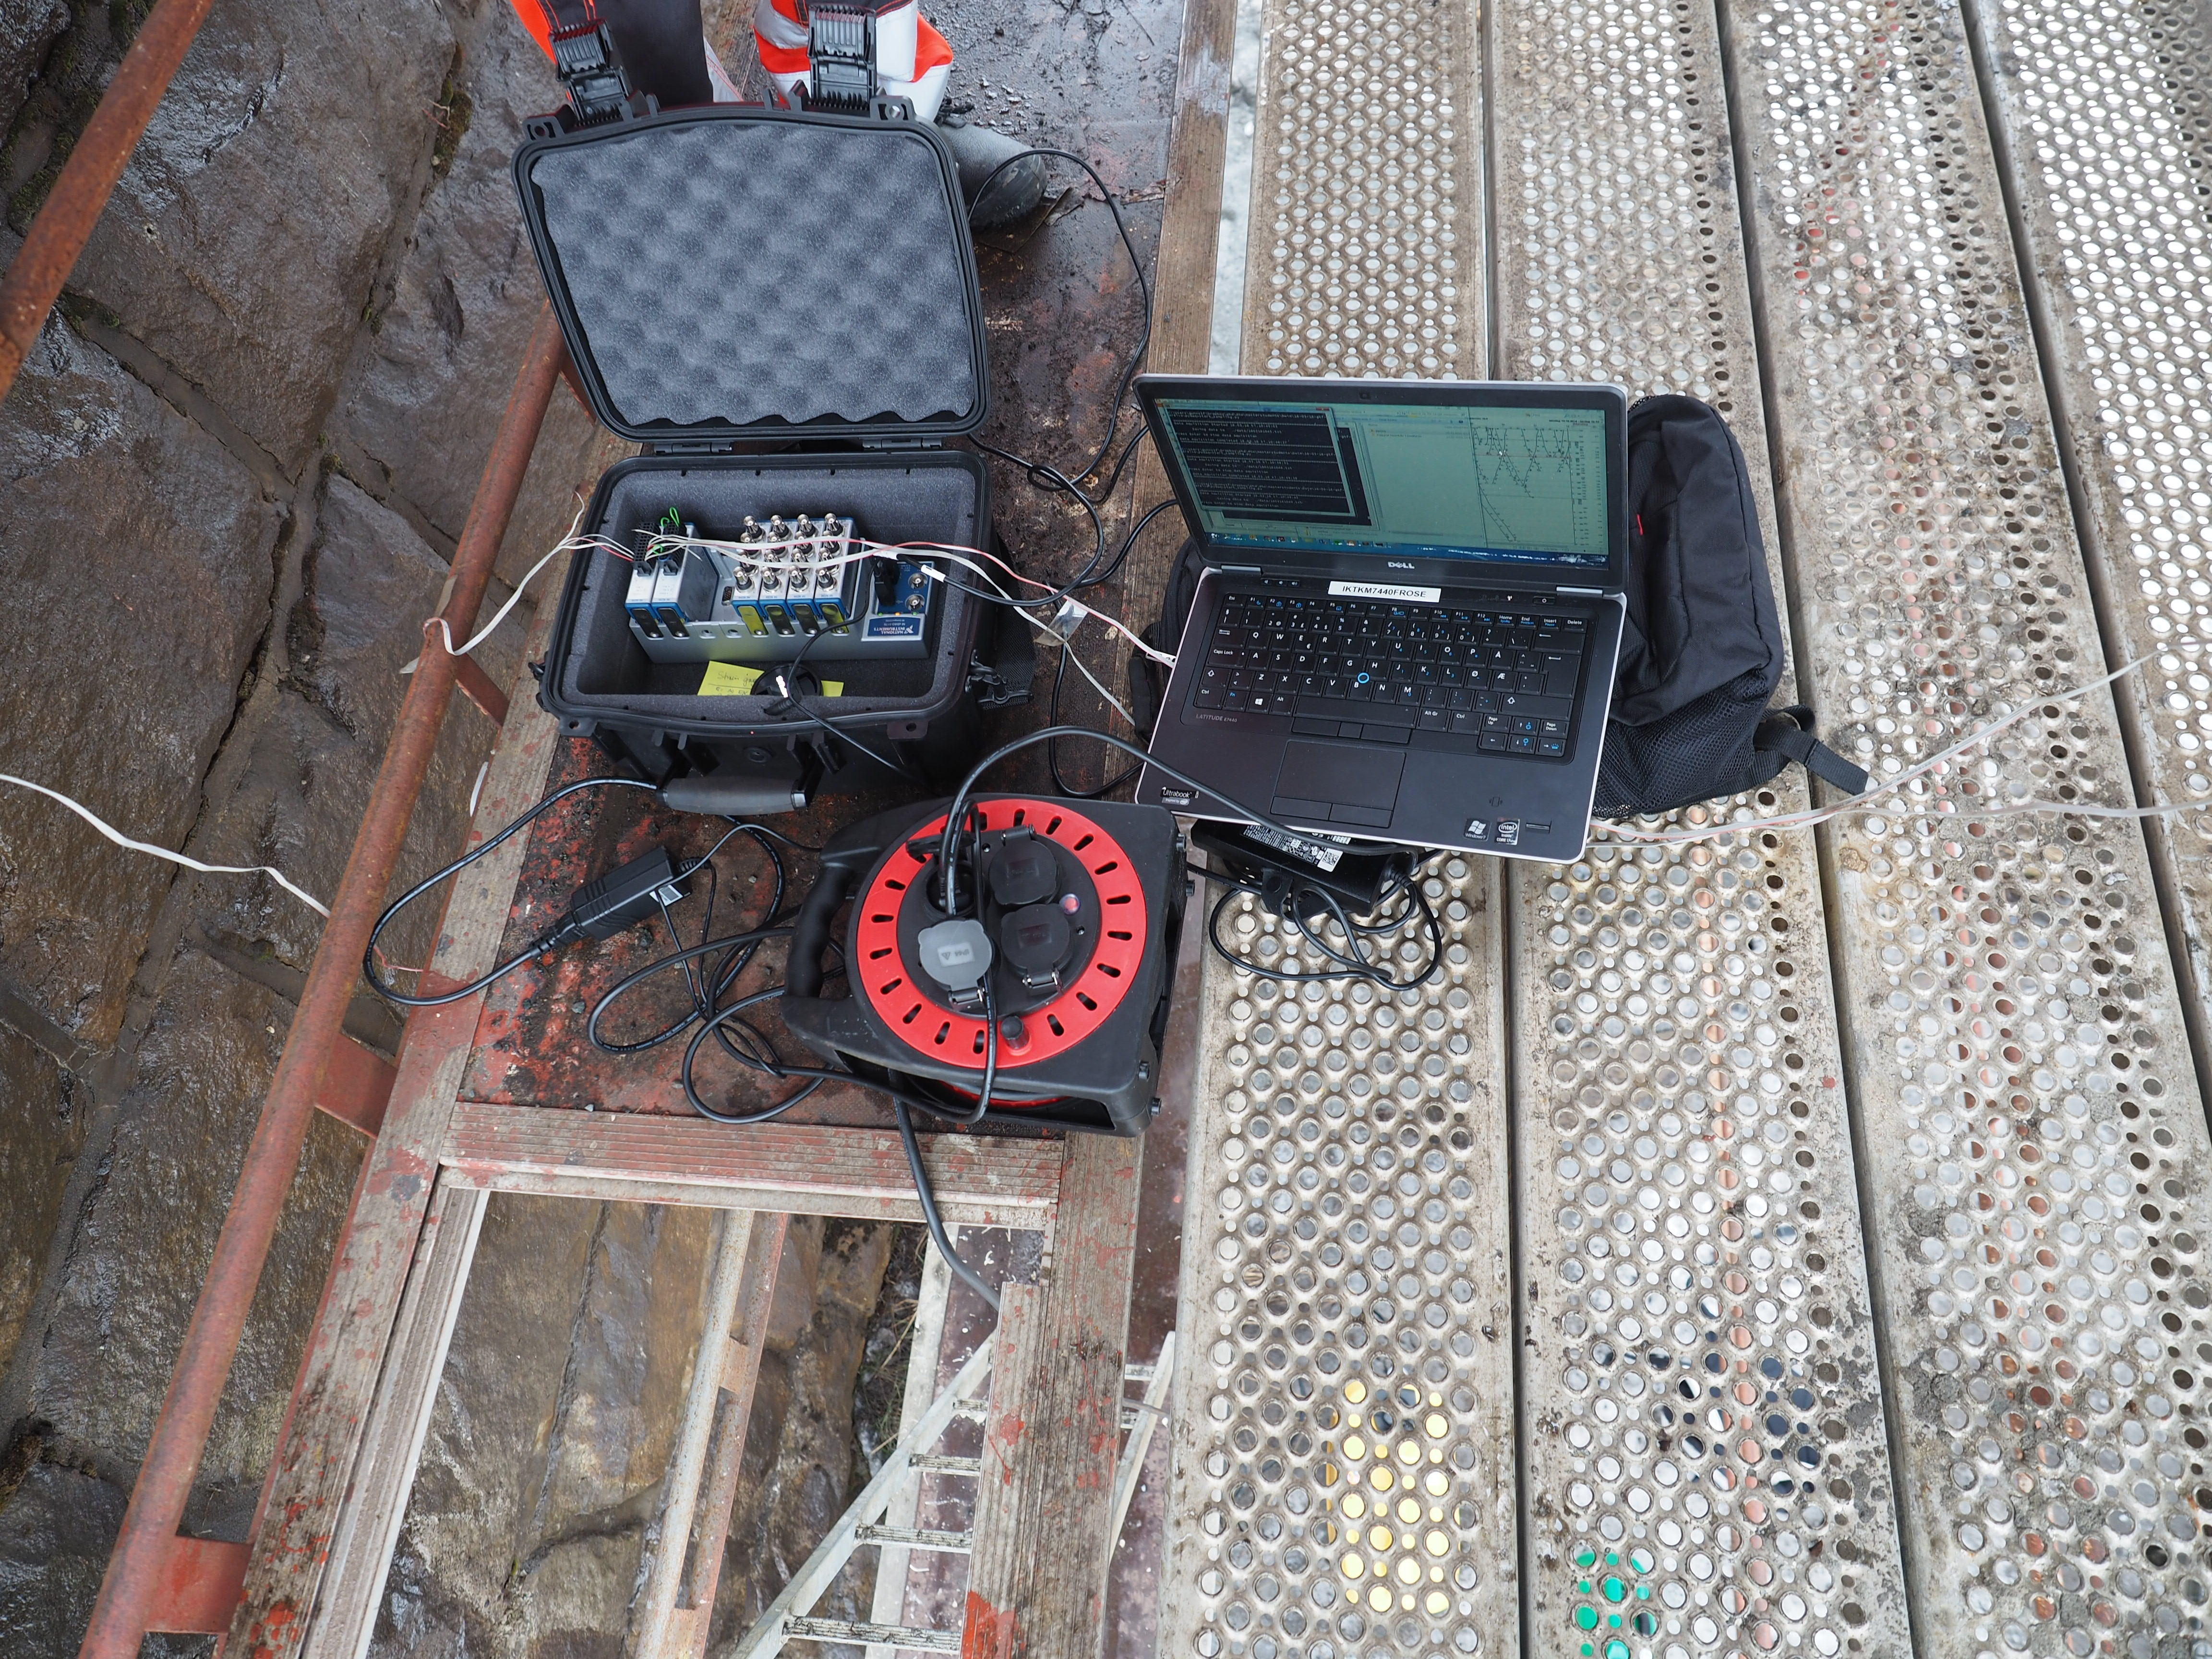
\includegraphics[width=\textwidth]{figures/system_setup}
		\caption{System setup from data gathering at Lerelva}
		\label{fig:instruments}
	\end{subfigure}
	\begin{subfigure}[t]{0.49\textwidth}
    \centering
    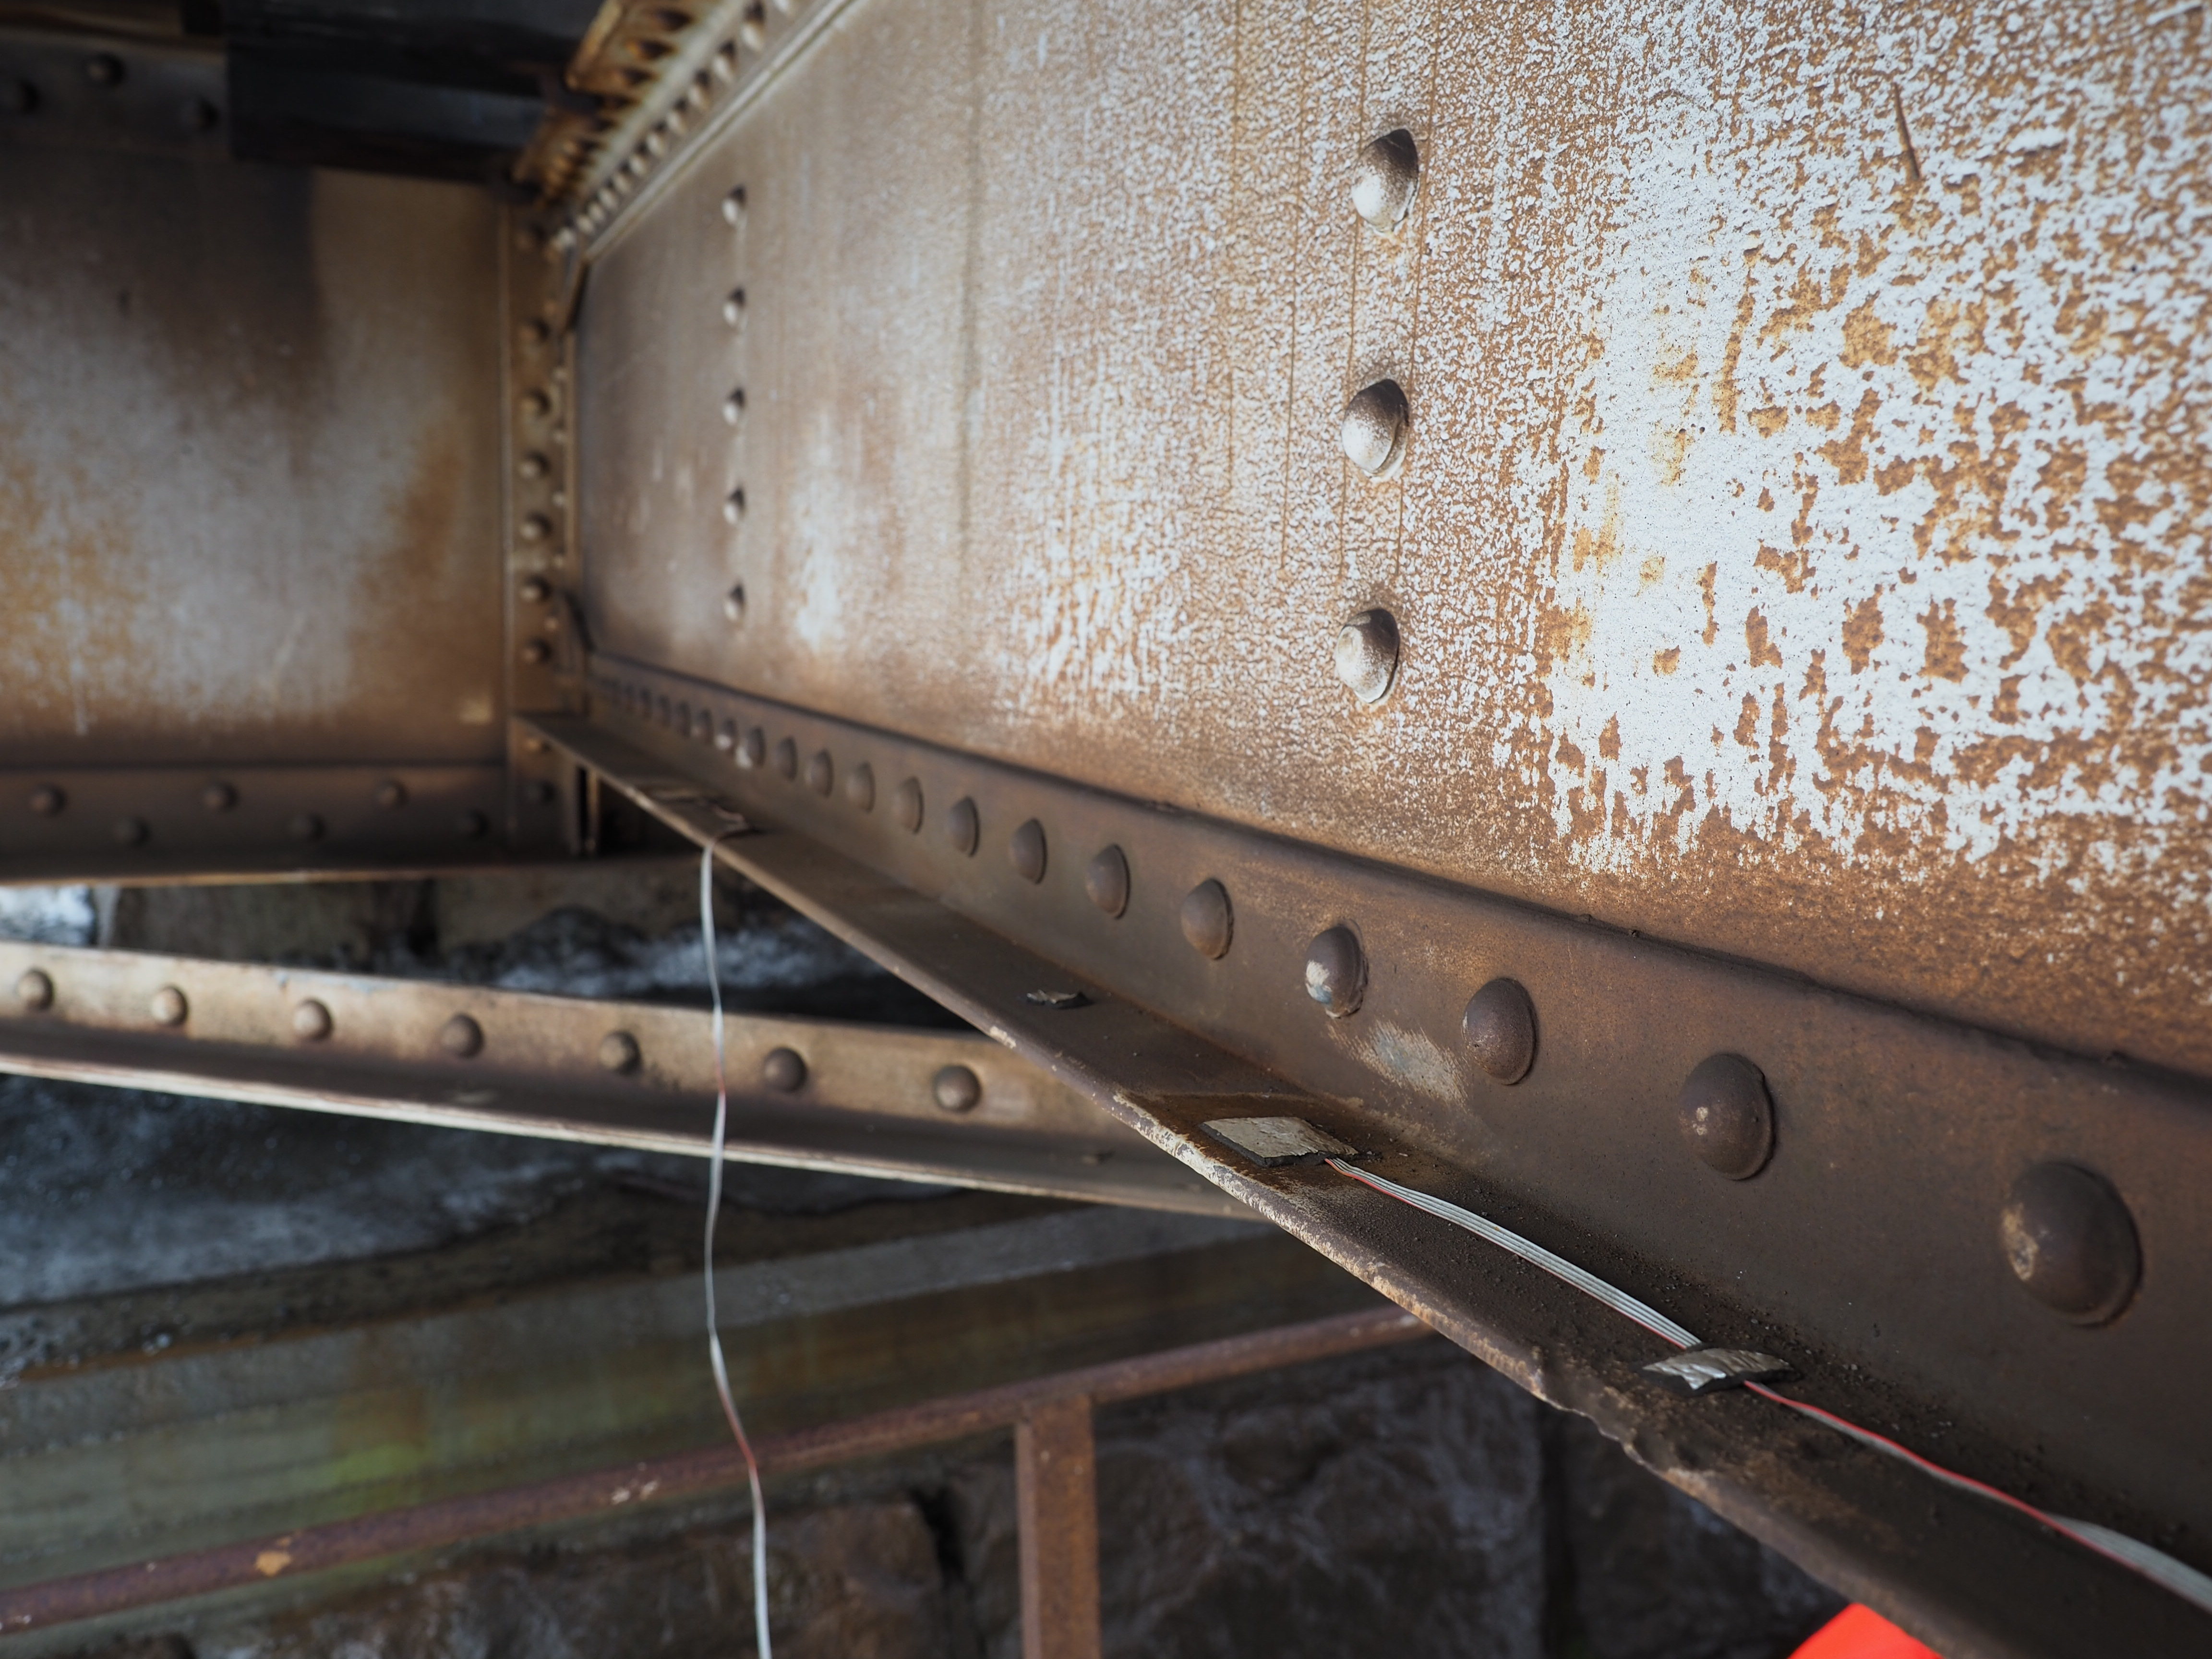
\includegraphics[width=\textwidth]{figures/sensor_placement}
		\caption{Placement of strain gauges on stringer section}
		\label{fig:strain_gauges}
	\end{subfigure}
	\caption{Instruments for aquiring strain data}
	\label{fig:system_setup}
	% 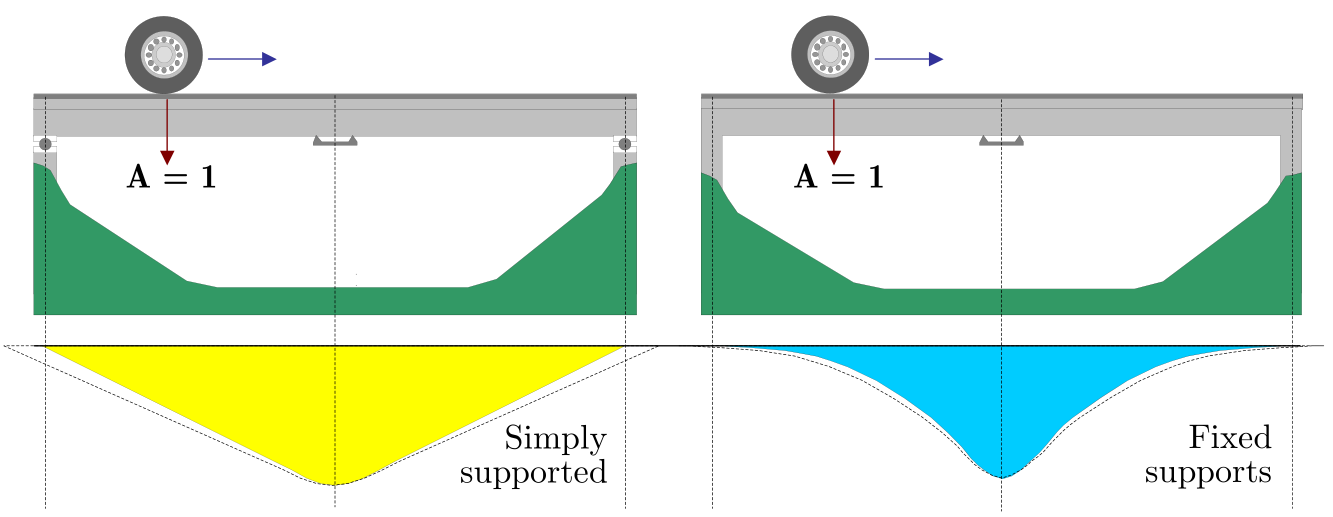
\includegraphics[scale=0.5]{figures/inflLinesQuilligan}
\end{figure}
\begin{figure}[H]
	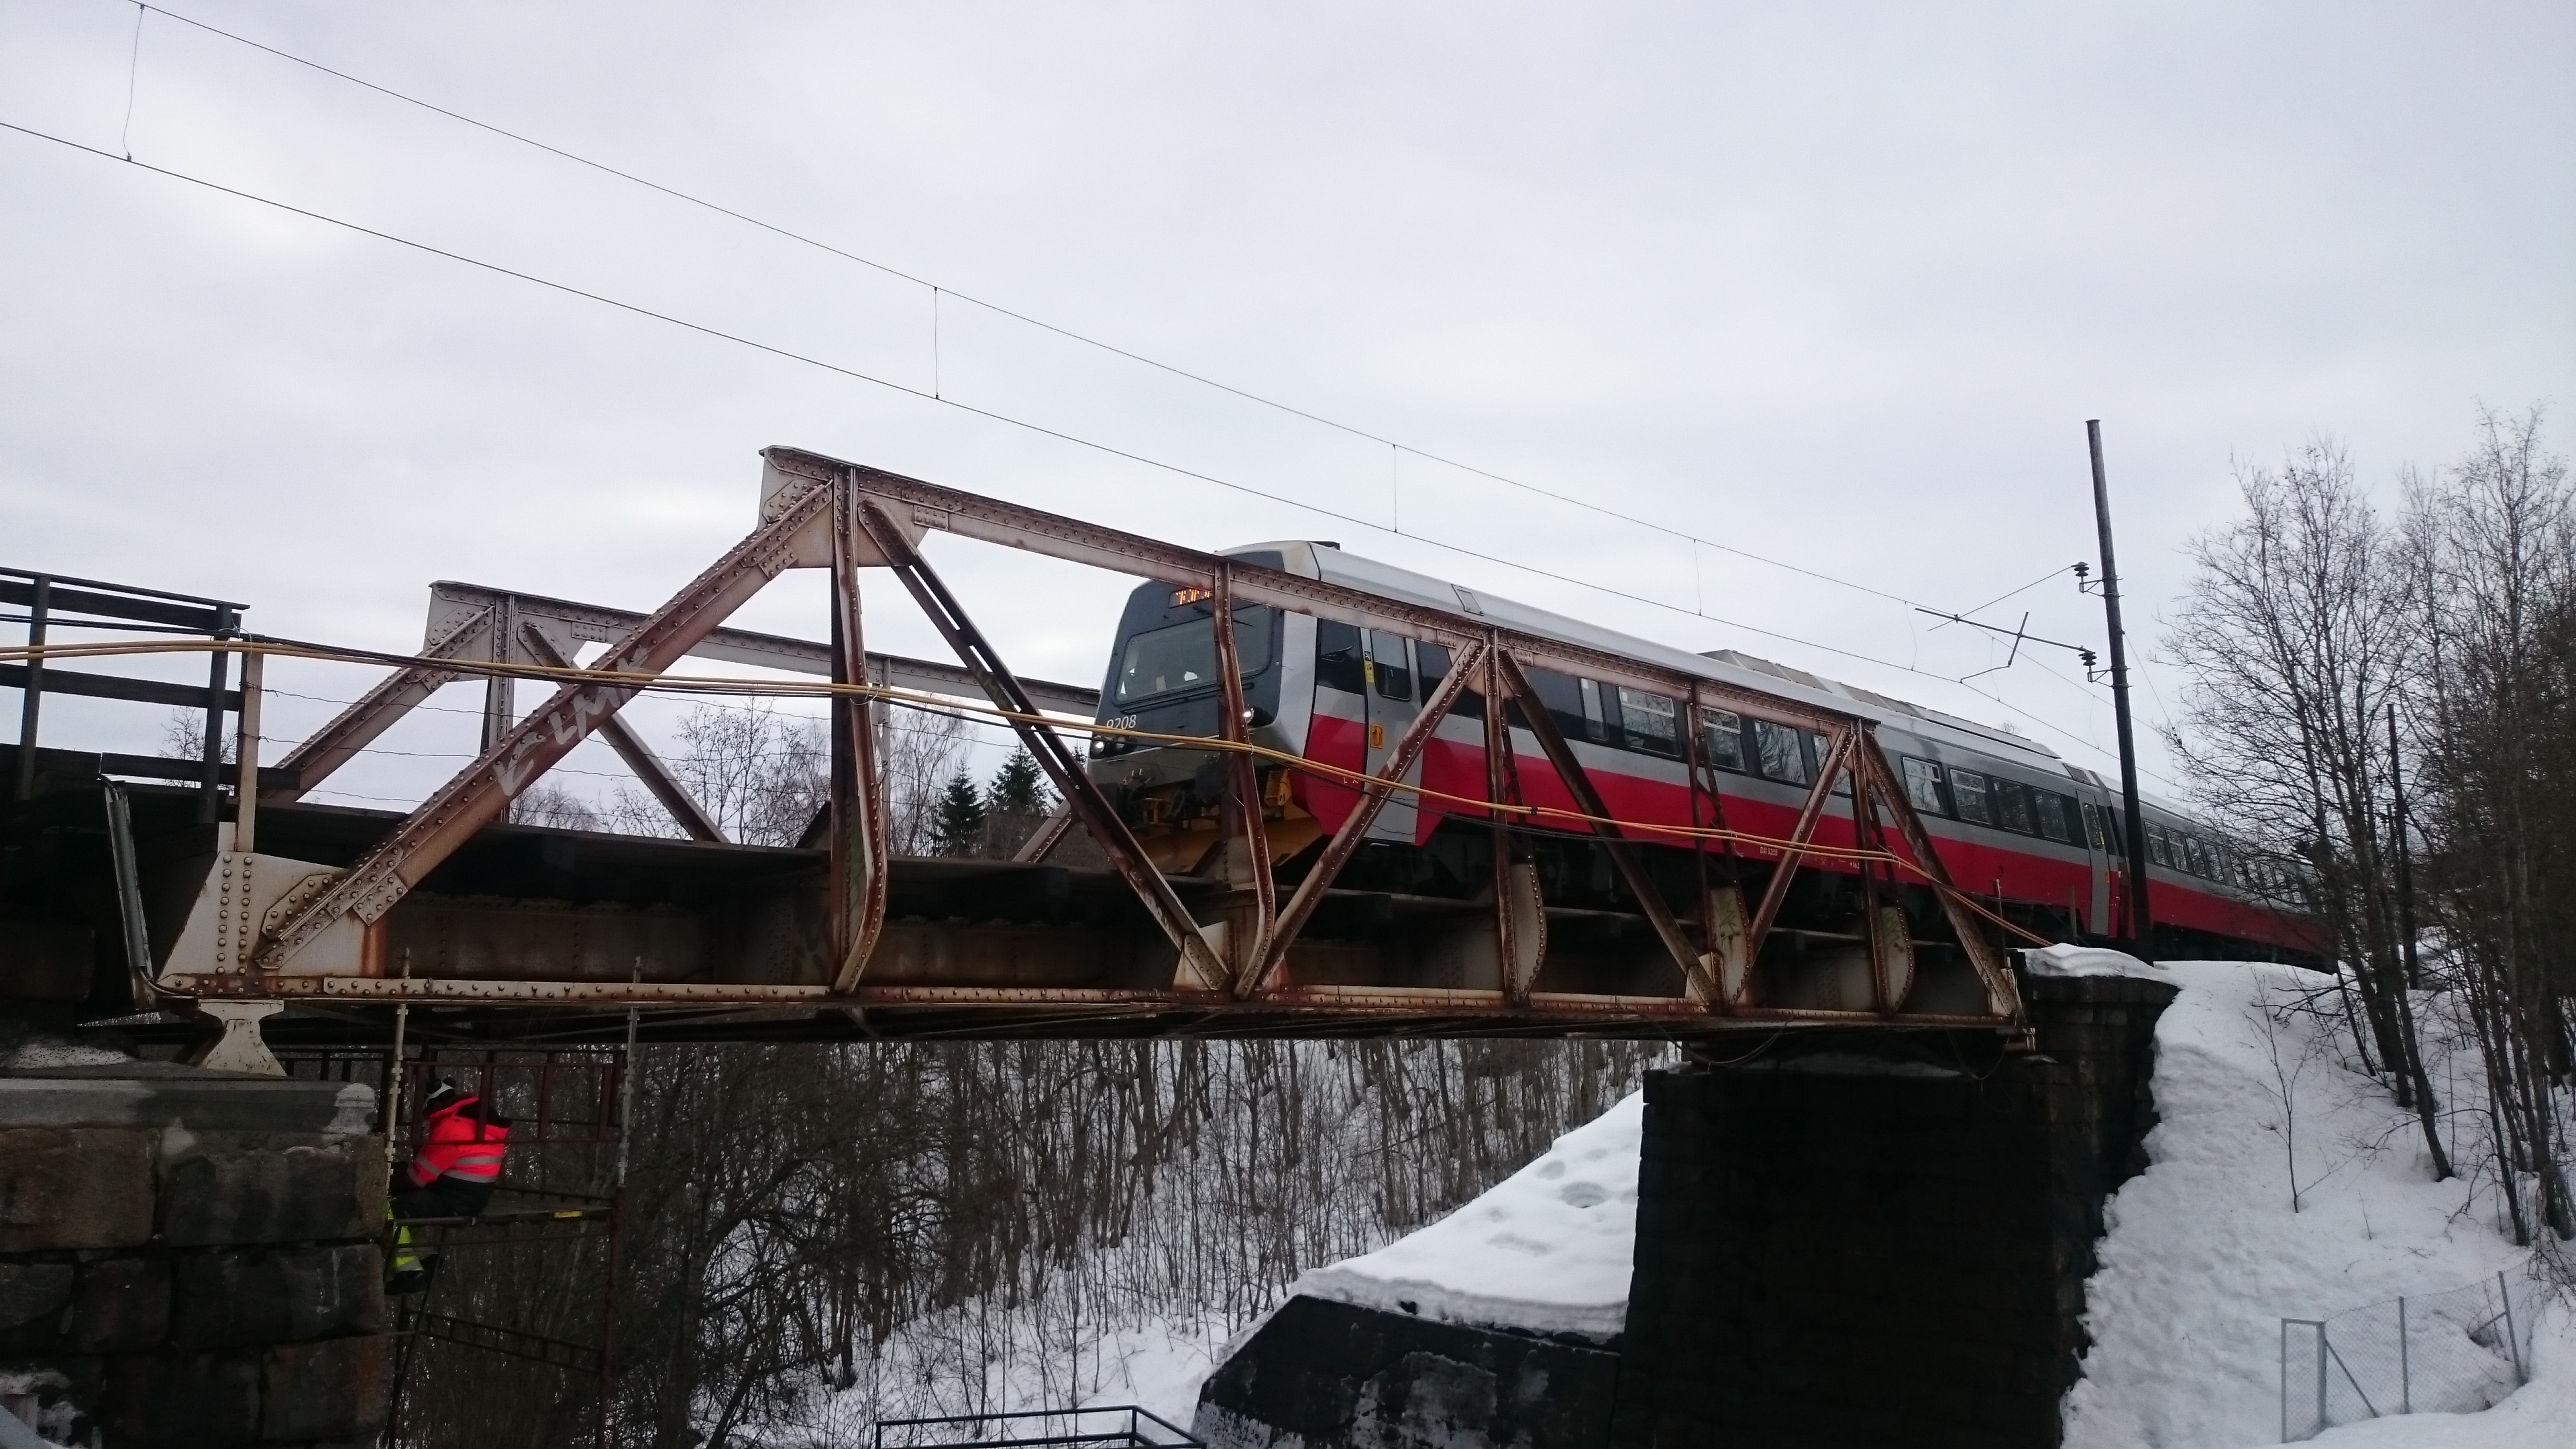
\includegraphics[width=\textwidth]{figures/train_passing.jpg}
	\caption{Lerelva bridge with a train passing over}
	\label{fig:lerelva_bridge}
\end{figure}

\begin{figure}[htpb]
	\begin{tikzpicture}
		\draw[thick] (0,0) to (9.9,0);
		\node[ledd fast={0}{0}{0}] (ledd) {};
		\node[ledd skyve={10}{0}{0}] (skyveledd) {};
		%\draw[->] (0,1) to {$\scriptstyle g$} (0,.1);
		% \node (a) at (0.0, 0.0) {};
		% \node (b) at (1.56,1.5) {};
		% \draw[thick] (a) to (b);
		\draw[thick] (0,0) to (1.65,1.5);
		\draw[thick] (1.65,1.5) to (3.3,0);
		\draw[thick] (3.3,0) to (4.95, 1.5);
		\draw[thick] (4.95,1.5) to (6.6, 0);
		\draw[thick] (6.6,0) to (8.25, 1.5);
		\draw[thick] (8.25,1.5) to (9.9, 0);

		\draw[thick] (1.65,1.5) to (4.95, 1.5); % Upper stringer
		\draw[thick] (4.95, 1.5) to (8.25,1.5); % Upper stringer
		\draw[thick] (1.65,0) to (1.65,1.5); % vertical
		\draw[thick] (3.3,0) to (3.3,1.5); % vertical
		\draw[thick] (4.95,0) to (4.95,1.5); % vertical
		\draw[thick] (6.6,0) to (6.6,1.5); % vertical
		\draw[thick] (8.25,0) to (8.25,1.5); % vertical
		\draw[-open triangle 90] (0,0) to node[above] {$Trondheim$} (-2.0,0);
		\draw[-open triangle 90] (9.9,0) to node[above] {$Heimdal$} (11.9,0);

		\filldraw
		(0.825,0) circle (2pt) node[align=left,   above] {s1};
		\filldraw
		(0.429,0) circle (2pt) node[align=left,   below] {s2};
		\filldraw
		(1.221,0) circle (2pt) node[align=left,   below] {s3};
	\end{tikzpicture}
	%\captionof{figure}{Beam model for initial BWIM}
	\caption{Sketch of bridge showing sensor locations for system setup at Leirelva bridge}
	\label{figure:systemSketch}
\end{figure}
\section{Data gathered}
The instruments discussed in \ref{system_setup}, provides a measurement frequency of 1024 Hz. All data was gathered the same system setup during a single day.
In all six trains were recorded passing the bridge. The system setup stored the signals for the three different sensors along with the time for the elapsed signals in a matrix for each train. The recordings of train passings were started and ended manually as no trigger was in place to start and end the signal. Some of the gathered signals therefore ended up being very long, which means it requires to have essential data extracted. One of the reccordings was also very short, but still usable.
Three of the trains travelled towards Heimdal, and three towards Trondheim.
For simplicity of the developement of the BWIM program this thesis assumes that the trains traversing Leirelva bridge does not accelerate or decelerate, while influencing the sensor.
\section{Trains}
\label{trains}
The trains recorded passing the bridge where of two types, a short two vagon commuter trains of type NSB92 as seen in figure \ref{appendix:nsb92} and a freight train with a EL14 locomotive as seen in \ref{figure:el14_locomotive}. The weight of the trains with passengers is unknown, resulting in axle weights being set equal the distibuted weight of the brutto train like shown in table \ref{table:axle_weights} obtained from \cite[p.~81]{lok_motorvogner}. For the freight train the properties of the locomotive was found through \cite{infoEL14}.
The axle distances was determined through figures \ref{appendix:nsb92} and \ref{figure:el14_locomotive}.
\begin{figure}[H]
	\begin{adjustbox}{center}
		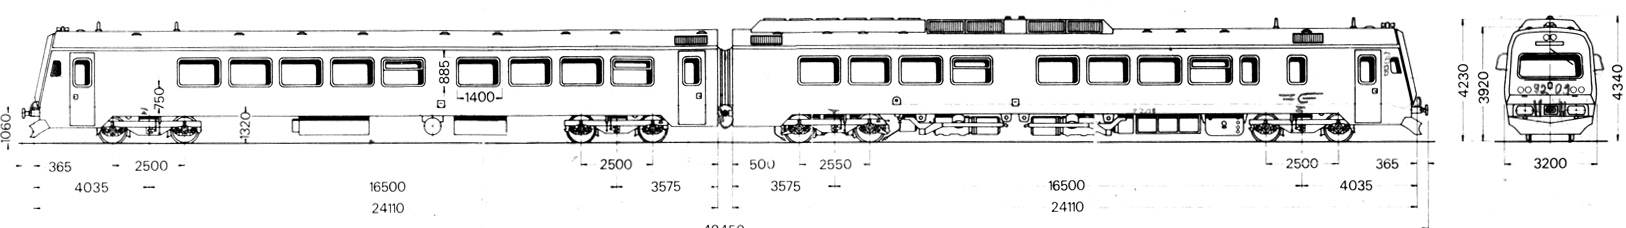
\includegraphics[width=0.8\pagewidth]{./figures/nsb92.png}
	\end{adjustbox}
	\caption{Axle distances of a NSB92 train}
	\label{appendix:nsb92}
\end{figure}

% \label{appendix:el14}
\begin{figure}[H]
	\begin{adjustbox}{center}
		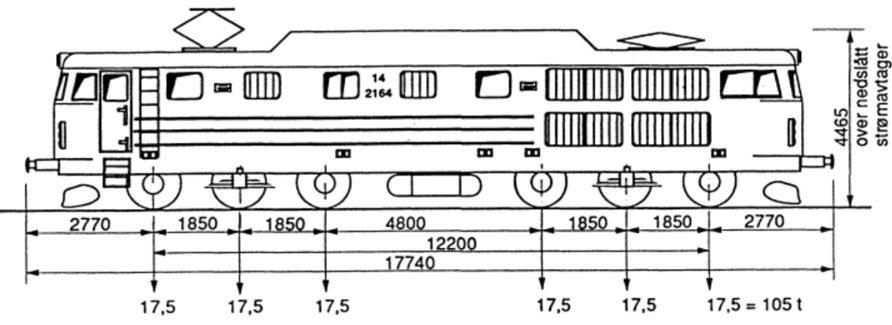
\includegraphics[width=0.8\pagewidth]{./figures/EL14.png}

	\end{adjustbox}
	\caption{Axle distances and weights for a EL14 locomotive}
	\label{figure:el14_locomotive}
\end{figure}

\begin{table}[h]
	\centering
	\begin{tabularx}{\textwidth}{ |X|X|X|X|X|X|X|X|X| }
		\hline
		Axle & 1 & 2 & 3 & 4 & 5 & 6 & 7 & 8 \\
		\hline
		Axle weight [\SI{}{\kg}] & 9500 &	9500 & 9500 &	9500 & 14575 & 14575 & 14575 & 14575 \\
		\hline
		sum  & \multicolumn{4}{ |c| }{38000} & \multicolumn{4}{ |c| }{58300} \\
		\hline
		sum total & \multicolumn{8}{ |c| }{96300} \\
		\hline
	\end{tabularx}
	\caption{Table of axle weights used to calculate Influence lines}
	\label{table:axle_weights}
\end{table}

% \begin{figure}[htpb]
% 	\begin{tikzpicture}
% 		\draw[thick] (0,0) to (10,0);
% 		\node[ledd fast={0}{0}{0}] (ledd) {};
% 		\node[ledd skyve={10}{0}{0}] (skyveledd) {};
% 		% \node[spring={3}{0}{0}] (spring) {};
% 		% \node[spring={6}{0}{0}] (spring) {};
% 		%\draw[->] (0,1) to {$\scriptstyle g$} (0,.1);
% 		\node (a) at (1,1.5) {};
% 		\node (b) at (1,.1) {};
% 		\draw[-open triangle 90] (a) to node[pos=-.4] {$axle 2$} (b);
% 		\node (c) at (3.5,1.5) {};
% 		\node (d) at (3.5,.1) {};
% 		\draw[-open triangle 90] (c) to node[pos=-.4] {$axle 1$} (d);
% 		\node (e) at (3.5,1) {};
% 		\node (f) at (4.5,1) {};
% 		\draw[-open triangle 90] (e) to node[pos=1.2] {$v$} (f);
% 		\node (g) at (1,.5) {};
% 		\node (h) at (3.5,.5) {};
% 		\draw[open triangle 90-open triangle 90] (g) to node[above] {$axle spacing$} (h);
% 		%\draw (2.5,0) circle [radius=0.1] {sensor};
% 		%\node[draw,circle] (s) at (2.5,0){};
% 		% \node[ledd fast={2}{0}{0}] (ledd) {};
% 		% \draw (2,-.75) -- (2.25,-1) -- (1.75,-1.25) -- (2.25,-1.5) -- (1.75,-1.75); % spring""
% 		\node[ledd spring={2}{0}{0}] (skyveledd) {};
% 		\node[ledd spring={4}{0}{0}] (skyveledd) {};
% 		\node[ledd spring={6}{0}{0}] (skyveledd) {};
% 		\node[ledd spring={8}{0}{0}] (skyveledd) {};
% 		\filldraw
% 		(2.5,0) circle (2pt) node[align=left,   below] {strain sensor};
% 	\end{tikzpicture}
% 	%\captionof{figure}{Beam model for initial BWIM}
% 	\caption{A more realistic beam bridge model}
% 	\label{figure:beam_model_alt}
% \end{figure}
